% Optional calls for page styles





\documentclass[12pt,letterpaper, openany]{book} %took out one side
%\usepackage[top=2cm, bottom=2cm, lmargin=3.5cm,rmargin=2.5cm,marginparwidth=6cm,marginparsep=2em]{geometry}

%PRINTING FORMAT
\usepackage[top=1.75cm, bottom=1.75cm, lmargin=3.25cm,rmargin=2.25cm,marginparwidth=6cm,marginparsep=2em, twoside]{geometry}

%ONLINE FORMAT
%\usepackage[top=1.75cm, bottom=1.75cm, lmargin=3.25cm,rmargin=2.25cm,marginparwidth=6cm,marginparsep=2em]{geometry}


%\setlength\parindent{0pt} %crush the auto indentation

%Footnote separation
\addtolength{\skip\footins}{1pc}

\reversemarginpar
\usepackage{import}
\usepackage{design}
\usepackage{preamble}

% Watermarking
%\usepackage{draftwatermark}


 
\usepackage{makeidx}
\makeindex


%% Above notes: You can remove twoside and replace with oneside in documentclass to have a better "online pdf" format. twoside is better for printing and binding. You may want to mess with margins to make this better for online viewing.
 
\begin{document}

% WATERMARK
%\SetWatermarkText{Property of Colin Roberts. NOT FOR REDISTRIBUTION.}
%\SetWatermarkColor[gray]{0.75}
%\SetWatermarkFontSize{1cm}
%\SetWatermarkAngle{45}
%\SetWatermarkHorCenter{10cm}
 
\frontmatter
% \noindent\makebox[\textwidth]{\rule{\textwidth}{0.4pt}}

% \huge{Math 255}

% \noindent\makebox[\textwidth]{\rule{\textwidth}{0.4pt}}

\begin{titlepage} % Suppresses headers and footers on the title page

	\centering % Centre everything on the title page
	
	\scshape % Use small caps for all text on the title page
	
	\vspace*{\baselineskip} % White space at the top of the page
	
	%------------------------------------------------
	%	Title
	%------------------------------------------------
	
	\rule{\textwidth}{1.6pt}\vspace*{-\baselineskip}\vspace*{2pt} % Thick horizontal rule
	\rule{\textwidth}{0.4pt} % Thin horizontal rule
	
	\vspace{\baselineskip} % Whitespace above the title
	
	{\LARGE Applied Mathematics for Chemists II} % Title
	
	\vspace{0.3\baselineskip} % Whitespace below the title
	
	\rule{\textwidth}{0.4pt}\vspace*{-\baselineskip}\vspace{3.2pt} % Thin horizontal rule
	\rule{\textwidth}{1.6pt} % Thick horizontal rule
	
	\vspace{2\baselineskip} % Whitespace after the title block
	
	%------------------------------------------------
	%	Subtitle
	%------------------------------------------------
	
	Vector fields, partial differentiation, cylindrical and spherical coordinates, multiple integrals, line integrals, the wave and the Schr\"odinger equations, separation of variables method. Inner Product Spaces. Fourier Series. % Subtitle or further description
	
	\vspace*{3\baselineskip} % Whitespace under the subtitle
	
	%------------------------------------------------
	%	Editor(s)
	%------------------------------------------------
	
	By
	
	\vspace{0.5\baselineskip} % Whitespace before the editors
	
	{\scshape\Large Colin Roberts \\} % Editor list
	
	\vspace{0.5\baselineskip} % Whitespace below the editor list
	
	\textit{Colorado State University} % Editor affiliation
	
	\vfill % Whitespace between editor names and publisher logo
	
	%------------------------------------------------
	%	Publisher
	%------------------------------------------------
	
	%\plogo % Publisher logo
	\begin{figure}[H]
	    \centering
	    
\includegraphics[width=.8\textwidth]{Frontmatter/ram_logo.jpg}
	\end{figure}
	
	\vspace{0.3\baselineskip} % Whitespace under the publisher logo
	
	Created in Spring 2020\\
    Updated in Spring 2021 % Publication year
	
% 	{\large publisher} % Publisher

\end{titlepage}


%No preface for now. Need a new one for 271.
%\section*{Preface}

This text was created to be a companion to the Math 255 - \emph{Calculus for Biological Students II} course at Colorado State University.  The reader is expected to have completed the Math 155 course with a solid grasp of the material in order for one to best absorb new topics in this course.

The aim of this text is to present relevant topics in \emph{multivariate calculus} and \emph{differential equations}.  To begin, one must learn some \emph{linear algebra}. Linear algebra provides a foundation that is required for studying functions of more than one variable.  It is also an extremely beautiful and applicable field of mathematics itself.  Vectors will serve as a generalization of the system of numbers one is already comfortable with.  With vectors, one can study systems that are naturally living in space.  We are already familiar with how functions can be applied to the real numbers, but they can also be applied to vectors living in space.  The simplest types of vector-functions are those that are \emph{linear}.  Given the simplicity, we often wish to understand more complicated functions by investigating their linear approximations.

Calculus studies the rate of change of functions, but it can be rephrased slightly.  Rather, we take the approach that calculus investigates the best linear approximations to functions.  With one variable, a function can be approximated by a tangent line with a slope found by computing the derivative. This is the best linear approximation to a function of one variable.  When functions input and output more than one variable, the derivative is thus a linear function. This slight rewording of the derivative definition allows for the analysis of functions defined in space and time much more naturally.  Of course, we also care about integration. Integration of functions with more than one variable allows for more types of integration.  That is, we can consider integration as a tool to find lengths of curves, areas, volumes, and other physically meaningful quantities.  

Many systems are easier to understand by studying how they change.  For example, if we push an object it accelerates; acceleration is the second derivative of the position function of an object.  In this case, the system is determined by rates of change and so the equation one writes down for this system is a differential equation.  To model systems that change over space and time, one must be able to write down and solve these differential equations.  Physical intuition can help guide one to a solution, but there are more surefire methods.  The main technique proposed is to simplify the problem just enough so that we can solve it more easily but not lose too much information.  Techniques from linear algebra continue to reemerge and allow us to solve a large class of (linear/first order) problems.  Other (nonlinear/higher order) problems can be simplified down to the case we work to solve.  Thus, we create quite a toolbox to investigate differential systems.


 
\clearpage
\thispagestyle{empty}
 
\tableofcontents
 
\mainmatter

\part{Prerequisites}
\chapter{Introduction \& Review}
    \section{Introduction}
    
    This class and the sequel are concerned with covering the mathematics of thermodynamics, electromagnetism, and quantum mechanics. Of course, the mathematics supplied here is not limited to these fields, but it is hopefully presented in a way to align with those subjects.  At the heart of chemistry are the interactions in and between atoms and molecules. On the small scale, their interactions and structures are entirely understood via experiment and quantum theory. Zoom out a bit and electromagnetic effects take over. Zoom out further and we find that ensembles of large amounts of chemicals behave due to thermodynamic or statistical mechanical laws.  
    
    All of scientific theory is verified by experiment, but the theory itself is based in mathematics. A working scientist tends to lean towards one side of the theory/experiment coin but should be knowledgeable in both respects.  Think of mathematical theory as providing you with another form of analysis.  Mathematical knowledge will undoubtedly help you in your future scientific endeavors.  At the very least, it is an exercise in how to approach problems in a logical way.
    
    Take this course as a first dive into many new areas of math.  There will \emph{immediately} be a wealth of new terms and methods presented to you.  Learning what these are takes effort.  Even keeping terminology correct or what type of object (scalar, vector, matrix, function, etc.) something is can be confusing! Keep your mind open to questions.  Try not to fear math and it will work with you. Keep your head up and do not feel discouraged when the material feels tough.  It is tough for everyone.  Eventually you will improve your understanding. After this course and the sequel, you can look back at everything you have learned and smile!
    
    
    \section{How to read this text}
    
    What good is a textbook if you don't enjoy reading it? Or worse, what if you can't follow the material? Reading textbooks can be challenging. Think of it as another step in your career of learning!
    
    To get the most out of this textbook I suggest the following:
    \begin{enumerate}
        \item \emph{Pre-read}. Read through the relevant section once and try to see what the main point is.  Don't fuss over details! Go for big picture here. Maybe write down questions that come to you.
        \item \emph{Re-read}. Read the relevant section again. Yes, I am asking for you to do this twice! This time, go slower. Go through with a fine tooth comb and make sure you can make as much sense of the material as you can.  See if all the logic is true.  If there are exercises, attempt them.  Write down questions and bring them to class, office hours, or to a tutor.
        \item \emph{Review}. Come to class, office hours, or meet with other students/colleagues/tutors to go over the questions you have. As this says here, class should be more of a review than a first pass through. Having questions is great! It means learning is soon to follow. 
        \item \emph{Practice}. Do the homework and work through other exercises present in the text. This is the start to mastering a subject.  You may feel that you have gotten the material down but you can't \emph{know} that until you try.  Give the homeworks a try without notes or the text until you feel you need it! This aids in ability to recall.
        \item \emph{Correct}. None of us are perfect. Chances are that you may still miss something on an exercise or problem that you were sure that you had right.  Realize the mistake and integrate the new knowledge.  Sometimes this takes a bit of un-learning.  That can be tough, so be patient and forgiving with yourself.
        \item \emph{Reference}. There will be times where you will need to revisit some previous material.  Use this text as a reference for our class.  The more times you see something, the more it will stick.
    \end{enumerate}
    
    Sometimes there will be information stored away in problems, exercises, questions, answers, or remarks that is not otherwise explained in the text.  This is done when a bit of information is better discovered by the reader as opposed to being given away.  These problems will typically be labeled with an asterisk to denote their importance. I choose to use the following conventions.
    \begin{itemize}
        \item \emph{Problems}. Not assigned to be turned in, but should be done to check your knowledge once you have spent time with a portion of the text.  Problems will come after sections or subsections and important problems are marked with an asterisk.
        \item \emph{Exercises}. Exercises come within the body of a section or subsection. These should be, at the very least, read along with the other material to see what can be asked. In general, these are not meant to take too long. They should mostly check your current understanding. Think of them as passage to the next material.
        \item \emph{Questions}. Questions are put there for you to think about.  Almost always the questions will come along with an answer. Though you have an answer, you should work to understand \emph{why} it is the answer and if there is any more to be said.
        \item \emph{Answers}. Given to most questions. Think about these and make sure they make sense to you.
        \item \emph{Remarks}. These have nuggets of information that serve as a reminder or notify the reader about some subtleties. Note what these remarks mention and be sure to keep them in mind.
    \end{itemize}
    
    \subsection{Mathematical language}
    
    \subsubsection{Mathematical symbols}

    Here is a list of symbols you will find in our class (if more come, I will update this list):

    \begin{itemize}
        \item $\R$, The set of \emph{real numbers}.
        \item $\in$, ``Is a member of." (i.e. $\sqrt{2}\in \R$ can be read as, ``The square root of 2 is a member of the real numbers."
        \item $\neq$, \underline{Not} equal to.
        \item $\approx$, ``Approximately equal to."
        \item $\coloneqq$, We are defining something, i.e., $\frac{df}{dx}\coloneqq \lim_{h\to 0}\frac{f(x+h)-f(x)}{h}$.
        \item $\implies$, "Implies."
        \item $\iff$, "If and only if."
        \item $\therefore~$, "Therefore."
        \item $\infty$, Infinity.  \emph{Note: Infinity is \underline{not} a number!}
        \item $\Delta$, A change. (i.e. $\Delta x$ represents a change in the variable $x$).
        \item $\mathbf{v}$, a boldfaced character will represent a vector.
        \item $(x_1,x_2,\dots,x_n)$, a vector with $n$ components.
        \item $\begin{bmatrix} x_1\\ x_2\\ \vdots \\ x_n\end{bmatrix}$, a vector with $n$ components.
    \end{itemize}
    
    \subsubsection{Mathematical presentation}
    
    I have provided you with some ideas on how to read this text which tend to be good practice in general.  But, this is a mathematics text, how is it different? Well, mathematics tends to be presented in a specific way and it can come across as being utterly devoid of inspiration.  In truth, mathematics is discovered almost entirely backwards from how a text is written.  It's just the truth.
    
    Like other mathematical texts, we will often motivate a topic and define some terms that seem to be helpful along the way.  It's sometimes easiest to add new terms to a dictionary when they are often used.  We just call this a \emph{definition}. See for example, Definition \ref{df:invertible_functions}. Definitions will be placed in CSU-themed green boxes.
    
    Definitions are tautologically true since we have defined the very thing we would like.  However, we sometimes wish to show that what we have defined plays nicely together and gives us some new useful information.  These can come in many forms!  We have \emph{theorems}, \emph{propositions}, \emph{lemmas}, and \emph{corollaries}; Each with its own specific meaning.  All of these results will be placed in CSU-themed gold boxes as they are representing new information. Let's briefly say what each is.
    
    \begin{itemize}
        \item \emph{Theorem}. An important logical result that needs proof to be accepted.  Proof comes from logic that we previously develop.  An example is the Pythagorean theorem.
        \item \emph{Proposition}. A smaller independent result, but important nonetheless.
        \item \emph{Lemma}. A smaller result that tends to be working towards a larger one.  Many times, a theorem is proved by using multiple lemmas beforehand.  
        \item \emph{Corollary}. A result that follows fairly easily from a lemma or theorem.  Sometimes it's extra emphasis on using a very general theorem on something more specific, so it is literally not saying anything new but rather pointing the reader to this important consequence.
    \end{itemize}
    
    In this journey of mathematics we will come across each one.  The important thing for the reader is to understand the logic along the way.  Do you need to prove theorems? No, I will do that for you. More often than not, I will even omit proofs unless they are strategically enlightening.  However, one should always be suspicious if some logic seems incorrect. I promise you, there are no lies in this text, but it doesn't mean things are obvious!
    
    
    \section{Review}
    The prerequisite classes for this course are Math 155, Math 159, or Math 160.  Moreover, there is a requirement that the following topics are understood.  To check your understanding, work through all the listed problems in this review section. I repeat! Work through each problem in the review! If you can work through each problem and, better yet, understand each step you take through a solution, then you are well on your way to learning new material in this course.
    
    This course will require the following:
    \begin{enumerate}[1.]
        \item Computation.
        \item Algebra.
        \item Geometry.
        \item Trigonometry.
        \item Functions.
        \item Calculus.
    \end{enumerate}
    
    \noindent Below in each respective subsection are notes and example problems.  
    
    \subsection{Computation}
    
    What is computation? Computation is what we have drilled into our heads at a young age.  It's how many of us view mathematics up until we explore areas such as algebra.  Given an expression, how can we interpret it?  With this, we also need an agreed upon language.
    
    Typically we mean to output a real (or possibly complex) number from an expression.\footnote{Really we just need outputs we agree upon. The numbers I mentioned are common but there's no inherent reason that those two number systems are what your expression calls for!} This number tells us what an expression means. For example, the expression is about making some type of measurement. In scientific fields, that is common.
    
    \subsubsection{PEMDAS}
    
    PEMDAS, or 
    \[
    \textrm{Parentheses $\veryshortarrow$ Exponents $\veryshortarrow$ Multiplication $\veryshortarrow$ Division $\veryshortarrow$ Division $\veryshortarrow$ Addition $\veryshortarrow$ Subtraction},
    \]
    gives the standard order of operations.  This is simply a choice us humans have agreed on and made calculators or computer programming languages follow.  Good for avoiding arguments, probably.
    
    The reason I note this here is so that we can pay attention to properly computing expressions.  Often times students will find expressions such as
    \[
    -2^2 \qquad \textrm{and} \qquad (-2)^2
    \]
    to be equal. If you found them equal, can you see how they differ?
    
    Be cognisant of what the expression is \emph{really} telling you to do.  Use calculators or online tools like Wolfram Alpha as tools to check your answers. Often you will not have have a calculator available, so practicing without one is ideal.
    
    \subsubsection{Logarithms and exponents}
    
    Logarithms and exponents are extremely important classes of functions as well as tools.  Logarithms originally assisted in helping mathematicians do large computations as they can turn multiplication into addition which is arithmetically less challenging.  Both show up in nature quite often.  Let us revisit the necessary rules we must know about these functions.
    
    For the following table, $\log$ represents a logarithm of any base.  A base is only specified when needed. Think about which rules are redundant, if any!
    \begin{table}[H]
        \centering
        \renewcommand{\arraystretch}{1.5}
        \begin{tabular}{c|c|c}
            Rule & Logarithms & Exponents\\
            \hline
            Identity & $\log(1)=0$ & $a^0=1$\\
            \hline
            Inverse & $\log_a\left(a^x\right)=x$ & $a^{\log_a(x)}=x$\\
            \hline
            Multiplication & $\log(ab)=\log(a)+\log(b)$ & $a^x a^y=a^{x+y}$ \\
            \hline
            Division & $\log\left(\frac{a}{b}\right)=\log(a)-\log(b)$ & $\frac{a^x}{a^y}=a^{x-y}$\\
            \hline
            Power & $\log(a^p)=p\log(a)$ & $\left(a^x\right)^p = a^{px}$
        \end{tabular}
        \label{tab:log_exp_rules}
    \end{table}
    \emph{Challenge}: Can you derive these rules based on what each function's definition is? That is, remember that
    \[
    a^p = \underbrace{aa\cdots a}_{p \textrm{~times}}
    \]
    \footnote{If $p$ is not a positive integer, this is a bit harder to understand. Pretend that it is for this case.}and
    \[
    b^x = a \quad \textrm{means that} \quad \log_b(a)=x.
    \]
    If you don't try this, that's okay.  One mathematical exercise is to re-derive knowledge for yourself. Many people find it helps the learning process immensely!
    
    Lastly, remember what the magnitude of different powers tell us.  That is, I want you to be comfortable making the following identifications.
    
    \begin{align*}
        a\cdot a &= a^2,\\
        \sqrt{a} &= a^{1/2},\\
        \sqrt[p]{a} &= a^{1/n},\\
        a^{-1} &= \frac{1}{a},\\
        a^{-p} &= \frac{1}{a^p}.
    \end{align*}
    
    Armed with your previous knowledge and the above information, work on the problems below.
    
    \subsubsection{Problems}
    
    \begin{problem}
    Evaluate the following.
    \begin{enumerate}[(a)]
        \item $-3^2-2(3+2^2)$;
        \item $(-3)^2-2(3+2)^2$;
        \item $\frac{2-(-3)^2}{2^{(3-2)^2}}$.
    \end{enumerate}
    \end{problem}
    
    \begin{problem}
    Write the following as a simplified fraction:
    \[
    \frac{1}{2}-\frac{3}{5}.
    \]
    \end{problem}
    
    \begin{problem}
    Rewrite the following in an equivalent way using log and exponent rules. If no rules apply, say so.
    \begin{enumerate}[(a)]
        \item $\ln(2a)$;
        \item $\ln(2+a)$;
        \item $\ln(2^a)$;
        \item $\log_{10}(a^2)$;
        \item $\log_2(2^a)$.
    \end{enumerate}
    \end{problem}
    
    \begin{problem*}
    Recall that we can convert between different bases of logarithms. For example,
    \[
    \log_a(x)=\frac{\log_b(x)}{\log_b(a)}.
    \]
    Convert the following logarithms to the \emph{natural logarithm} (logarithm with base $e$) and evaluate the expression when possible.
    \begin{enumerate}[(a)]
        \item $\log_2(2)$;
        \item $\log_2(8)$;
        \item $\log_8(2)$;
        \item $\log_{10}(e)$;
        \item $\log_3(1)$;
        \item $\log_5(0)$.
    \end{enumerate}
    If an expression can't be evaluated, can you explain why?
    \end{problem*}
    
    \begin{remark}
    The name ``natural logarithm" will make more and more sense as we see how natural Euler's Number $e$ is.
    \end{remark}
    
    \begin{problem*}
    We can also convert between different bases for exponentials. Really, we just like to do this to convert to the exponential with Euler's number $e$. We have that
    \[
    b^x=e^{\ln(b)x}.
    \]
    Can you show this using the rules above? Convert the following to their natural exponential ($e^\textrm{something}$) counterpart or convert to the form $b^x$.
    \begin{enumerate}[(a)]
        \item $3^x$;
        \item $e^{\ln(2)x}$.
    \end{enumerate}
    \end{problem*}
    
    \subsection{Algebra}
    
    What is algebra? Algebra is Arabic for ``reunion of broken parts." It is a large and pervasive field of mathematics concerned with structure.  There are many different flavors as well.  Abstract algebra, linear algebra, and operator algebra are just a few examples. We will learn some of each of the named fields as we progress through the Math 271 and 272 courses.
    
    At this point, we treat algebra as manipulation of equations.  What one does to one side of an equation must do to the other in order to keep from changing the result or truth.  We are all familiar with this concept.  Clearly if 
    \[
    x=5
    \]
    and I only add $2$ to the right side,
    \[
    x=5+2=7,
    \]
    then our knowledge about $x$ has changed.  Albeit a simple example, this is \emph{exactly} what happens when we make algebra mistakes in our work.  Believe me, \emph{all} of us make algebra mistakes. 
    
    Practice with the problems below to review your understanding of algebra. They are given in no particular order.  Algebra is unbelievably fundamental in our pursuit of mathematical knowledge. We must make sure to have a strong foundation! 
    
    \subsubsection{Problems}
    
    \begin{problem}
    Solve the equation for $p$:
    \[
    3p-(5-2p)=2(p-3).
    \]
    \end{problem}
    
    \begin{problem}
    Solve the equation for $x$:
    \[
    12<\frac{9-x}{3}.
    \]
    \end{problem}
    
    \begin{problem}
    Which number(s) $x$ are in the interval $[2,6)$ and satisfy $x<4$?
    \end{problem}
    
    \begin{problem}
    Simplify the following.
    \[
    \frac{a^3b^4}{(ab)^2}=?
    \]
    What can we say if $a$ or $b$ is equal to zero?
    \end{problem}
    
    \begin{problem}
    Show that the following equalities are true using the rules given on exponents, fractional, and negative powers.
    \begin{enumerate}[(a)]
        \item $\displaystyle{\sqrt{x^2+x^2y^2}=x\sqrt{1+y^2}}$
        \item $\displaystyle{\frac{x^2+y^2}{x}=x+\frac{y^2}{x}}$
    \end{enumerate}
    \end{problem}
    
    
    \subsection{Geometry}
    
    What is geometry? Loosely speaking, geometry is the study of shape of space.  Geometry is concerned with distances, angles, size, and shape.  Many tools from more advanced geometry are distilled into a form that we will use throughout the time in Math 271 and Math 272.  At times, we will explore some of these concepts in a more advanced way (see linear algebra and multivariate calculus).
    
    For an introduction, knowing planar and spatial geometry is helpful.  One should be familiar with calculating areas and volumes as well as lengths and angles. The most important shapes to recognize will be circles and triangles as they satisfy some nice symmetries or properties.  We can use these two shapes along with some trigonometry to make geometrical inference.
    
    Here are some common volumes that may show up in Math 271 or the sequel, Math 272.
    
    \begin{figure}[H]
        \centering
        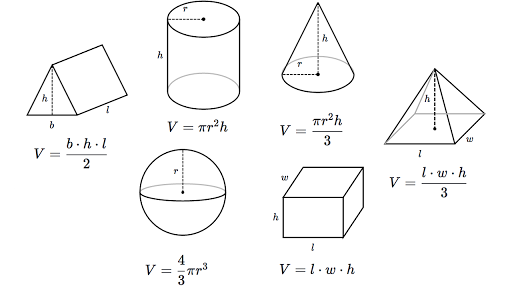
\includegraphics[width=.8\textwidth]{Figures_Part_1/volumes.png}
        \label{fig:volumes}
    \end{figure}
    
    % \subsubsection{Problems}
    
    
    % \begin{problem}
    % Compute the area of the following
    %     \begin{tikzpicture}
    %     \centering
    %     \draw[line width=1pt](0,0)--(3,1);
    %     \draw[line width=1pt](0,0)--(0,2);
    %     \draw[line width=1pt](0,2)--(3,1);
    %     \end{tikzpicture}
    % \end{problem}
    % areas, volumes, circles, triangles
    
    \subsection{Trigonometry}
    
    What is trigonometry? Think of trigonometry as the mathematics behind analyzing planar triangles and circles.  This comes down to using the well known trigonometric functions $\cos$, $\sin$, $\tan$, $\sec$, $\csc$, $\cot$. Of course, we often times care about the (pseudo) inverse functions of these as well. 
    
    One of the most important results in trigonometry is the Pythagorean Theorem. We will use it all throughout this course in one way or another.  Let us state it below. 
    
    \begin{thm}{Pythagorean Theorem}{pythag}
    Let $\triangle$ be a right triangle with side lengths $a$, $b$, and $c$ shown below.
    \begin{figure}[H]
        \centering
        
\includegraphics[width=.3\textwidth]{Figures_Part_1/right_triangle.png}
    \end{figure}
    Then we have that $c^2=a^2+b^2$.
    \end{thm}
    
    % \textcolor{blue}{Degrees and radians, cosines, sines of angles and what they represent. Why a circle has $2\pi$ radians. We can compute distances in the plane using pythagorean}
    
    % \subsubsection{Problems}
    
    
    \subsection{Functions}
    
    What are functions? Functions are machines that give a single output for a given input. This is something you may have heard called the ``vertical line test" when you were looking at graphs of real values functions. But, Beware! That doesn't mean that each single input corresponds to a single output. Many inputs can have the same output. More on this later.
    
    We often use functions to represent relationships or measurements.  Analyzing functions is of utmost importance when we wish to gain insight from them.  For us, functions will typically be thought of as some physical variable (think temperature, velocity, or probability). We'll also learn that functions can be solutions to certain kinds of expressions called \emph{differential equations}.  
    
    There is a lot of terminology and notation surrounding functions. Let us cover the necessary details. 
    
    \subsubsection{Notation and terminology}
    
    We typically represent a function (of a single variable) by $f(x)$ and say ``$f$ of $x$." Of course, the function $f$ and input $x$ can be represented by any symbols you'd like.  Maybe you want to have a function $\smiley(\uparrow)$ which we would say ``smiley of up-arrow." We tend to stick with notation others use to stay a bit more sane.
    
    Mathematicians really like to specify a function by writing
    \[
    f\colon D \to C
    \]
    which can be read as ``$f$ inputs variables from the set $D$ and sends them into the set $C$." Here, $D$ is the \emph{domain} and $C$ is the \emph{codomain}. This notation is handy when we deal with functions that have different inputs and outputs than we have handled before. So, mathematicians shouldn't be the only ones to like this notation!
    
    So far, what I have provided above does not specify what the function actually does.  For this, we usually provide an expression like
    \[
    f(x)=x^2
    \]
    which tells us to square each input to get the output or we can specify the function to take certain values when given a certain input, i.e.,
    \[
    f(2)=3.
    \]
    
    
    \subsubsection{Domain, codomain, and range}
    
    The domain and range of a function are always specified. However, sometimes the specification is understood and we don't list it.  The \boldgreen{domain}\index{domain} $D$ of a function is the set of all input values.  The \boldgreen{codomain}\index{codomain} $C$ of a function is the set that output values can live in.  \emph{Note, \underline{not} all elements in the codomain are necessarily output by the function!} The \boldgreen{range}\index{range} $R$ of a function is the set of all output values.  
    
    \begin{question}
    Is the codomain $C$ a larger, smaller, or same size set as the range $R$?
    \end{question}
    
    \begin{answer}
    This was a bit of a trick question.  The codomain is \emph{at least as big} as the range as it contains all the output values the function \emph{could} hit.  The range may have the same exact elements of the codomain and the range could be smaller than the codomain.
    \end{answer}
    
    \begin{ex}{Codomain and Range for Finite Sets}{codomain_range}
    \begin{enumerate}[(i)]
        \item Let $f$ be a function with domain $D=\{1,2,3\}$ (i.e., $D$ is the set of numbers one, two, and three) and codomain $C=\{1,2,3,4\}$. We can say that 
    \[
    f\colon D \to C
    \]
    and we completely define $f$ by choosing an output for each input. We'll take
    \begin{align*}
        f(1)&=1;\\
        f(2)&=1;\\
        f(3)&=4.
    \end{align*}
    As stated, the codomain is the set $\{1,2,3,4\}$, but what is the range $R$? Since we have specified an output for every input, we can just look at the list of outputs which is
    \[
    f(1)=1,~f(2)=1,~f(3)=4,
    \]
    and so the range $R=\{1,4\}$.  Notice that the range is strictly smaller than the codomain. Also, this function does \underline{not} output a unique value for each given input.
    
        \item Let $g$ be a function on the same domain and codomain as in (i). That is,
        \[
        g\colon D \to C.
        \]
        Let us define $g$ as we did with $f$ by specifying the output for each input.
        \begin{align*}
            g(1)&=2;\\
            g(2)&=3;\\
            g(3)&=4.
        \end{align*}
        Again, one should check that the range is smaller than the codomain. Also, check whether this function has a unique output for each input. 
    \end{enumerate}
    \end{ex}
    
    \begin{question}~
    \begin{itemize}
        \item Given an output value for the function $g$ above, can one determine what the input value had to be?
        \item How about for $f$?
        \item What is the difference between these two? 
    \end{itemize}
    \end{question}
    
    \begin{answer}~
        \begin{itemize}
            \item Yes we can. We call this association the \emph{inverse function}.
            \item No, not quite.  For example, what input gives us the output value of 1?
            \item $g$ is a \emph{one-to-one} function. It has a unique input value for each output value. $f$ is \underline{not} one-to-one.  Inverting $f$ is not really possible.
        \end{itemize}
    \end{answer}
    
    \begin{ex}{Codomain and Range for $\R$-Functions}{codomain_range_real}
        Let us work with functions we are likely more familiar with.  
        \begin{enumerate}[(i)]
            \item Let $f$ be a real valued function of one real variable. That is, 
            \[
            f\colon \R \to \R.
            \]
            We understand this as $f$ takes in a real value and outputs a real value as well.  This is just some extra notation and verbage for something we already understand!
            
            Since $\R$ is infinite, us humans can't really specify an output value for every input.  Instead, we provide an association.  Let's define $f$ by saying what $f$ \emph{does} to some input value.  Let
            \[
            f(x)=x^2.
            \]
            Now, the codomain for $f$ is all the real numbers $\R$ but the range $R$ for $f$ is smaller.  Since we are squaring the input to get the output, the range of $f$ is $R=[0,\infty)$.  We can't achieve negative values! Notice also that $f$ is not one-to-one.
            
            \item Let's define a new function $g\colon \R \to \R$ by letting
            \[
            g(x)=x^3.
            \]
            The range in this case is $\R$ and $g$ is one-to-one. You should verify these facts.
        \end{enumerate}
    \end{ex}
    
    
    \subsubsection{Composition}
    
    If we have functions $f$ and $g$, we may want to look at how we can string the two together.  First, we should say what we mean by this and determine when it is even possible to do so.  Let's say that we have
    \begin{align*}
        f\colon D_1 &\to C_1,\\
        g\colon D_2 &\to C_2,
    \end{align*}
    and the range for $f$ and $g$ is $R_1$ and $R_2$ respectively.  We want to consider the composition of functions
    \begin{align*}
        (f\circ g)(x) &= f(g(x)),\\
        (g\circ f)(x) &= g(f(x)).
    \end{align*}
    
    \begin{question}
    When are we allowed to \emph{compose} the function $f$ with $g$ as $f\circ g$? How about as $g\circ f$?
    \end{question}
    
    \begin{answer}
    Let's think of this in an analogy.  If $f$ converts from Spanish to English and $g$ converts from German to Spanish, how can we string the two translators together to convert from German to English?  
    
    Think of $x$ as a word in German.  If we then look at $g$ translating $x$,
    \[
    g(x)=y,
    \]
    then $y$ is now some word in Spanish.  Now, $f$ is happy to translate this word right on over to English by
    \[
    f(y)=z,
    \]
    where $z$ is our desired English word.  So, we have really done the following:
    \[
    (f\circ g)(x)=f(g(x))=f(y)=z.
    \]
    
    Now, in terms of functions on sets of numbers, we want to think like in this above analogy.  The output of one function $g$ better agree with the input $f$ knows how to handle.  More below.
    \end{answer}
    
    If we have that the range $R_1$ is in the domain $D_2$, then we can have the composite function
    \[
    g\circ f,
    \]
    and
    \[
    g\circ f \colon D_1 \to C_2.
    \]
    This may be fairly abstract and confusing.  Don't worry too much! We'll keep seeing the point of this way of thinking over time. Let this knowledge grow slowly over time.
    
    \begin{exercise}
    Repeat the above if we have that the range $R_2$ is in the domain $D_1$.
    \end{exercise}
    
    \subsubsection{Inverse functions}
    
    We have all seen \emph{inverse functions}, but let us re-familiarize ourselves with them just a bit while also giving a preview of the style of text to come.
    
    \begin{df}{Invertible Functions}{invertible_functions}
    Let $f\colon D \to C$ be a function. We say that $f$ is \boldgreen{invertible}\index{invertible} if for any value $y\in C$ there is a corresponding unique input $x\in D$.  That is to say, if we have $f(x)=y$ then the inverse function, $f^{-1}$, satisfies
    \[
    f^{-1}(y)=x.
    \]
    The inverse function \emph{undoes} the original function. So we have that
    \[
    (f^{-1}\circ f)(x)=x
    \]
    and
    \[
    (f\circ f^{-1})(y)=y.
    \]
    for every $x$ and every $y$.
    \end{df}
    
    \begin{remark}
    There's more subtleties here than meets the eye.  I'm going to avoid them for now.  But if you'd like more to think about, consider the composition function
    \[
    f\circ f^{-1}.
    \]
    What will we have to know about domains, ranges, or codomains? Careful.
    \end{remark}
    
    Alluded to earlier was the idea of a function that is one-to-one. Let's define that here and now.
    \begin{df}{One-to-one Function}{one_to_one}
    Let $f\colon D \to C$ be a function. We say that $f$ is \boldgreen{one-to-one} if for each output value $y$ there is a unique input value $x$.
    \end{df}
    \noindent Take a moment to soak this one in. Revisit Example \ref{ex:codomain_range} and Example \ref{ex:codomain_range_real}. Think of a few examples of functions that are and are \underline{not} one-to-one.
    
    Another important notion is that of a function whose range is equal to the codomain.  We made sure to see that there could be differences before, so let's define this notion.
    
    \begin{df}{Onto Function}{onto_fxn}
    Let $f\colon D \to C$ be a function with range $R$. If we have $R=C$, then $f$ is \boldgreen{onto}\index{onto}.
    \end{df}
    
    While we're at it, we may as well introduce a proposition. This is not a groundbreaking result as the definitions we have really play nicely together. 
    
    \begin{prop}{One-to-one and Onto Functions are Invertible}{one_to_one-invertible}
    \textit{If $f\colon D \to C$ is a one-to-one and onto function if and only if it is also invertible.}
    % \noindent \emph{Proof.} Suppose the $f$ is one-to-one, then we know that for each output $y$, there is a unique input $x$.  Thus, we can define an inverse function that, given the input $y$, assigns an output $x$. That is, we make $f^{-1}(y)=x$, which is indeed a function since for each input we have a unique output. Thus, $f$ is invertible.
    
    % For the converse, we suppose that $f$ is invertible and we have $f^{-1}$ as the inverse function.  Since $f^{-1}$ is a function, it must assign a unique output value for each input.  This means that $f$ must only assign a unique output for each unique input, or else this could not be trust. Hence, it follows that $f$ is one-to-one. \qed
    \end{prop}
    Right now, we're avoiding any proof.  This one isn't too bad, but I'll restate that proofs are not part of this course. Proofs take time to understand and it's challenging to develop the skills to write them properly!  That's why the mathematics majors at CSU take Math 235 as an introduction to mathematical reasoning.  It truly is a challenge in its own right.
    
    
    \subsubsection{Visualizing functions}
    When working with real valued functions of one real variable (again, $f\colon \R \to \R$), we often draw the \emph{graph} of the function in the plane.  The function knows nothing about how we like to look at it, and it's important to realize that this is merely a human adaptation.  We'll eventually learn \emph{exactly} what it is that we do when we graph a function, but give it time.  For the mean time, just revisit the idea yourself.
    
    \begin{ex}{Graphing a Function}{graphing_function}
    Let's consider the function $f\colon \R \to \R$ given by $f(x)=x^2$.  The the \boldgreen{graph}\index{graph} of $f$ is the set of points $(x,f(x))$ that we highlight in the $xy$-plane.  So, the graph for this $f$ follows.
    \begin{center}
    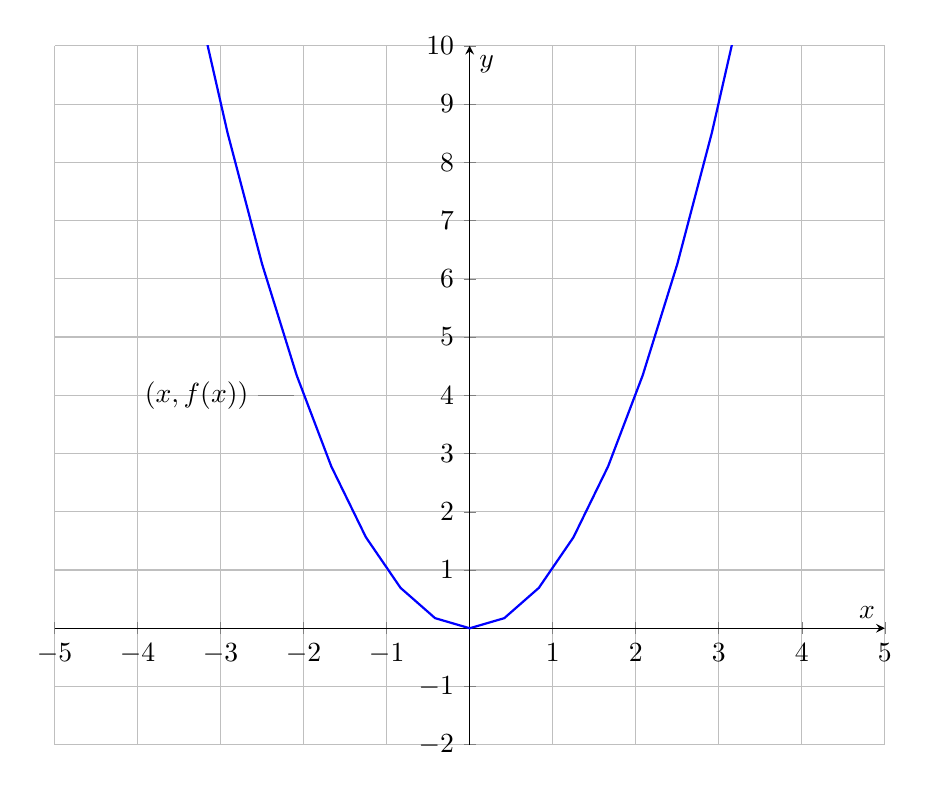
\begin{tikzpicture}[baseline]
    \begin{axis}[
    axis y line=center,
    axis x line=middle,
    %axis equal,
    grid=both,
    xmax=5,xmin=-5,
    ymin=-2,ymax=10,
    xlabel=$x$,ylabel=$y$,
    xtick={-10,...,10},
    ytick={-10,...,10},
    width=\textwidth,
    anchor=center,
    ]
    \addplot [mark=none, blue, thick]{x^2} ;
    \addplot [mark=none] coordinates {(-2,4)} node[pin=180:{$(x,f(x))$}]{};
    \end{axis}
    \end{tikzpicture}
    \end{center}
    \end{ex}
    
    Similar techniques for visualizing functions in higher dimensions will come. For now, just practice with functions of one real variable.
    
    \subsubsection{Problems}
    
    \begin{problem}
    Let $f(x)=x^2$. 
    \begin{enumerate}[(a)]
        \item Show that
        \[
        f(x+y)=x^2+2xy+y^2.
        \]
        \emph{Warning!} There is a common error made here. Do not fall victim to believing that
        \[
        f(x+y)=f(x)+f(y)
        \]
        for \underline{all} functions.  Functions that have this property are \emph{special}!
        \item Show that
        \[
        f(\lambda x)=\lambda^2x^2.
        \]
    \end{enumerate}
    \end{problem}
    
    \begin{problem}
    Let $g(r)=\frac{\hbar}{2}(r+r^2)$. Evaluate and simplify the following.
    \begin{enumerate}[(a)]
        \item $g(a+b)$;
        \item $g(\lambda a + x)$;
        \item $g(r^2)$.
    \end{enumerate}
    \end{problem}
    
    \begin{problem}
    Let $r(\smiley)=\frac{1}{\smiley^2}$. Evaluate and simplify the following.
    \begin{enumerate}[(a)]
        \item $\left[r(\smiley)\right]^2$;
        \item $r(-\smiley)$;
        \item $-r(\smiley)$.
        \item $r(\smiley)+r(2\smiley)$.
        \item $r(\smiley)+2r(\smiley)$.
        \item $r(\smiley^2)+r(2\smiley)+2r(\smiley)$.
    \end{enumerate}
    \end{problem}
    
    \begin{remark}
    Just remember, the function and variable letters are arbitrary. Pay attention on how to properly evaluate a function with a given input despite aesthetic differences.
    \end{remark}
    
    \begin{problem}
    Find the domain and range of $f(x)=\sqrt{9-x}$.
    \end{problem}
    
    \begin{problem}
    Find the domain and range of $h(t)=\sqrt[3]{2-x^2}$.
    \end{problem}
    
    \begin{problem}
    Let $f(x)=5x+1$ and $g(x)=x^2$.
    \begin{enumerate}[(a)]
        \item Write the composite function $(g\circ f)(x)$.
        \item Write the composite function $(f\circ g)(x)$.
    \end{enumerate}
    \end{problem}
    
    \begin{problem}
    Use the table to find $(f\circ g)(3)$
    \begin{center}
    \begin{tabular}{|c||c|c|c|c|c|c|}
        \hline
        $x$ & -2 & -1 & 0 & 1 & 2 & 3 \\
        \hline
        $f(x)$ & 0 & 6 & 4 & -1 & 3 & -2\\
        \hline
        $g(x)$ & 5 & 3 & 2 & 1 & -1 & 0\\
        \hline
    \end{tabular}
    \end{center}
    \end{problem}
    
    \begin{problem}
    State if the given functions are inverses of each other. Be sure to check both $(f\circ g)$ and $(g\circ f)$ to see that this is true.
    \begin{enumerate}[(a)]
        \item $\displaystyle{f(x)=4-\frac{3}{2}x}$ and $g(x)=\displaystyle{\frac{1}{2}x+\frac{3}{2}}$;
        \item $f(x)=11x-2$ and $\displaystyle{g(x)=\frac{x+2}{11}}$.
    \end{enumerate}
    \end{problem}
    
    \begin{problem}
    Find the inverse for the following functions. If one does not exist, explain why. If a domain isn't specified, assume that it is $\R$.
    \begin{enumerate}[(a)]
        \item $f(x)=x^3$.
        \item $g(x)=x^2$.
        \item $h(x)=\sqrt{x}$.
        \item $l(x)=8x+3$.
        \item $p(x)=\sqrt[3]{x}-3$.
    \end{enumerate}
    \end{problem}
    
    
    
    \subsection{Calculus}
    
    So far, all of us have studied the calculus of functions of one real variable.  It just so happens that the techniques developed there will generalize nicely to higher dimensional cases.  However, it will take some careful thought along the way.  What's the point anyway?
    
    Calculus is the study of rates of change of functions.  I like to think about it as the study of functions on the very small scale.  On the small scale, you found that functions look almost linear.  It's not hard to see this!  Take any function of your liking and zoom in on a specific region of this function. Keep zooming in and you'll notice that at some point the function looks like a line.  This idea allowed us to look at the \emph{derivatives} of functions as well as help us compute \emph{integrals} of functions!  It's extremely important.  It will also relate to a beautiful field of mathematics known as linear algebra. 
    
    Studying change is about all we ever do as scientists.  Even systems that \emph{don't} change over time can be thought of as just having no rate of change! As we turn knobs or mix chemicals we watch for change. We record this change and study the properties both before and after.  It is undoubtedly important for all of us to know a nice way to analyze changes of systems. This is captured elegantly by calculus.
    
    \subsubsection{Derivatives}
    \emph{Derivatives} were introduced to study change of functions.  First, we looked at average rates of change of functions over an interval.  Say we have a function $f\colon \R \to \R$ and we want to find its average rate of change from $x_0$ to $x_1$, then we would compute
    \[
    \frac{\Delta f}{\Delta x} = \frac{f(x_1)-f(x_0)}{x_1-x_0}.
    \]
    But, what if we make this interval very \emph{very} small?  We would then be looking at functions on this very small scale where, graphically, they look like lines. As the interval shrank to zero, or we took
    \[
    \lim_{x_1 \to x_0} \frac{f(x_1)-f(x_0)}{x_1-x_0},
    \]
    we arrive at an instantaneous rate of change.
    
    Recall that a \boldgreen{derivative}\index{derivative} is the instantaneous rate of change of a (single variable) function. We defined the derivative $f'$ of $f$ at the point $x$ to be
    \[
    f'(x)\coloneqq\lim_{\Delta x \to 0} \frac{f(x+\Delta x)-f(x)}{\Delta x}.
    \]
    Can you see how the the two limits given are the same? We also had the notation
    \[
    \frac{d}{dx}f(x)=f'(x),
    \]
    which is nice to use at times. It will be especially helpful in the future to use the latter (Leibniz) notation.  Recall also that we had a handful of derivative rules.  Keep these near and dear to your heart.
    
    
    %Consider using longtable here somehow
    \begin{table}[H]
        \centering
        \renewcommand{\arraystretch}{2.5}
        \begin{tabular}{c|c}
            Rule & Derivative\\
            \hline
            Sum & $\displaystyle{\frac{d}{dx}(f(x)+g(x))=f'(x)+g'(x)}$\\
            \hline
            Constant Multiple & $\displaystyle{\frac{d}{dx}(c f(x))=cf'(x)}$\\
            \hline
            Product & $\displaystyle{\frac{d}{dx}(f(x)g(x))=f'(x)g(x)+f(x)g'(x)}$\\
            \hline
            Quotient & $\displaystyle{\frac{d}{dx}(f(x)/g(x))}=\frac{f'(x)g(x)-f(x)g'(x)}{\left[g(x)\right]^2}$\\
            \hline
            Chain & $\displaystyle{\frac{d}{dx}f(g(x))=f'(g(x))g'(x)}$\\
            \hline
            Power & $\displaystyle{\frac{d}{dx}x^p=px^{p-1}}$\\
            \hline
            Log & $\displaystyle{\frac{d}{dx}\ln(x)=\frac{1}{x}}$\\
            \hline
            Exponential & $\displaystyle{\frac{d}{dx}e^x=e^x}$\\
            \hline
            Sine & $\displaystyle{\frac{d}{dx}\sin(x)=\cos(x)}$\\
            \hline
            Cosine & $\displaystyle{\frac{d}{dx}\cos(x)=-\sin(x)}$
        \end{tabular}
        \label{tab:der_rules}
    \end{table}
    These will be all the necessary rules to know moving forward.  This list is actually quite redundant. Can you see which you can find from others?
    
    
    \subsubsection{Integrals}
    \emph{Integration} is the other fundamental technique learned in an introductory calculus course.  The idea is to be able to add up function values over an interval. This helped to also develop the ability to find area under a curve.  There are a few things to note here.
    
    Remember that an \boldgreen{integral}\index{integral} can be in the form of \boldgreen{definite integrals}\index{integral!definite} or as \boldgreen{indefinite integrals}\index{integral!indefinite}. The former returns a number that tells one the \emph{net} area under the graph of function.  Indefinite integrals, on the other hand, return a function that we so joyfully refer to as the \boldgreen{anti-derivative}\index{anti-derivative}. 
    
    We have some integration rules as well, but it is a shorter list. For now.
    \begin{itemize}
        \item Sum rule: $\displaystyle{\int f + g dx=\int f dx + \int g dx}$.
        \item Constant multiple rule: $\displaystyle{\int cf dx = c \int f dx}$.
    \end{itemize}
    
    There is one important theorem that we all need to remember here and before we begin a new voyage.  That is the following.
    
    \begin{thm}{Fundamental Theorem(s) of Calculus}{ftc}
    Let $f\colon [a,b] \to \R$ be a differentiable function with derivative $f'$.  Then we have the following:
    \[
    \int_a^b f'(x)dx = f(b)-f(a).
    \]
    
    We can also say that 
    \[
    \int f'(x)dx = f(x)+c
    \]
    for some constant $c\in \R$ as well as
    \[
    \frac{d}{dx} \int f(x)dx = f(x).
    \]
    \end{thm}
    \noindent This theorem is very fundamental to the study of calculus, hence the name!
    
    One should be familiar with how to perform \emph{integration by substitution} or a \emph{$u$-substitution}. That is, given an integral of the form
    \[
    \int_a^b f(g(x))g'(x)dx
    \]
    one can make a substitution letting $u=g(x)$ and noting that $du=g'(x)dx$.  Of course, many integrals are not of this form, but surprisingly many are. Anyways, we find that with this substitution we have
    \[
    \int_a^b f(g(x))g'(x)dx= \int_{g(a)}^{g(b)}f(u)du.
    \]
    
    \begin{ex}{Integration by Substitution}{int_by_sub}
        Consider the definite integral
        \[
        \int_1^2 2x\sin\left(x^2\right)dx.
        \]
        Notice that the $2x$ looks like the derivative of the inside of $\sin\left(x^2\right)$.  So we let $u=x^2=g(x)$ and we have $du=2xdx$. Thus we have
        \begin{align*}
            \int_1^2 2x\sin\left( x^2\right)dx &= \int_1^4 \sin(u)du\\
            &= -\cos(4)+\cos(1).
        \end{align*}
    \end{ex}
    
    After this technique comes one that may not be seen in any prerequisite course for this class.  This new technique is known as \emph{integration by parts}. Integration by parts is a combination of the derivative product rule and the fundamental theorem of calculus.  Given functions $u(x)$ and $v(x)$ we can write
    \[
    (uv)'=u'v+uv'.
    \]
    Then if we integrate both sides, we have
    \[
    \int_a^b (uv)'dx = \int_a^b u'vdx + \int_a^b uv'dx.
    \]
    Fundamental theorem of calculus gives us that
    \[
    \int_a^b (uv)'dx = u(b)v(b)-u(a)v(a)
    \]
    and thus
    \[
    \int_a^b u'vdx = u(b)v(b)-u(a)v(a)-\int_a^b uv'dx.
    \]
    Or, without bounds on the integral, we can write
    \[
    \int u'vdx = uv - \int uv'dx.
    \]
    I like to think of integration by parts as shifting the derivative from one function to another with a penalty term.  Above, we swap a derivative on $u$ to a derivative on $v$ but have to correct with the function $uv$.  This can all be derived in higher dimensions using Stokes' theorem. It's an excellent tool in the study of differential equations.
    
    \begin{ex}{Integration by Parts}{int_by_parts}
        Consider the indefinite integral
        \[
        \int xe^x dx.
        \]
        Now $x$ is a function that gets ``simpler" when we take a derivative since $\frac{d}{dt}x= 1$.  So we wish to pick $v=x$ so $v'=1$ and hence $u'=e^x$ and we then have $u=e^x$ as well.  Plugging this in, we find
        \begin{align*}
            \int xe^x dx = \int u'vdx &= uv - \int uv'dx\\
            &= xe^x-\int_e^xdx\\
            &= xe^x - e^x + c.
        \end{align*}
    \end{ex}
    
    \subsubsection{Problems}
    
    \begin{problem}
    Compute derivatives for the following functions.
    \begin{enumerate}[(a)]
        \item $f(x)=18x^3+2x^2$;
        \item $g(x)=\sqrt{x+5}$;
        \item $h(x)=\sqrt{\frac{1}{x}}$;
        \item $p(x)=\sqrt[5]{x^3+15x}$;
        \item $q(x)=\frac{1}{\sqrt[4]{2x}}$;
        \item $r(x)=\sqrt{x^2}$. \emph{Hint: You can't cancel the square root and the square as they are \underline{not} proper inverses! Is this function differentiable everywhere? Plot it if need be.}
    \end{enumerate}
    \end{problem}
    
    \begin{problem}
    Compute derivatives for the following functions.
    \begin{enumerate}[(a)]
        \item $f(x)=xe^x$;
        \item $g(x)=e^{2x}$;
        \item $h(x)=b^x$;
        \item $p(x)=(x^2+2x)\ln(x)$;
        \item $q(x)=\ln\left(\frac{1}{x}\right)$;
        \item $r(x)=x^x$. \emph{Hint: This is tough. Try taking a natural log of both sides before differentiating.}
    \end{enumerate}
    \end{problem}
    
    \begin{problem}
    Compute derivatives for the following functions.
    \begin{enumerate}[(a)]
        \item $f(x)=\tan(x)$;
        \item $g(x)=\sec(x)$;
        \item $h(x)=\csc(x)$;
        \item $p(x)=\cot(x)$;
        \item $q(x)=\tan(\sin(\cos(x)))$.
    \end{enumerate}
    \end{problem}
    
    \begin{problem}
    Compute the following.
    \begin{enumerate}[(a)]
        \item $\displaystyle{\frac{d}{dx}\left(15y+15x\right)}$;
        \item $\displaystyle{\frac{d}{dy}\left(15y+15x\right)}$;
        \item $\displaystyle{\frac{d}{dr}\left(15y+15x\right)}$;
        \item $\displaystyle{\frac{d}{dx}\left(5x^2y+32y^3+5xy^2\right)}$;
        \item $\displaystyle{\frac{d}{dy}\left(5x^2y+32y^3+5xy^2\right)}$.
    \end{enumerate}
    \end{problem}
    
    \begin{problem}
    Compute the following antiderivatives. \emph{Do not forget the $+c$!}
    \begin{enumerate}[(a)]
        \item $\displaystyle{\int 2xdx}$;
        \item $\displaystyle{\int \cos(x)dx}$;
        \item $\displaystyle{\int \sec^2(x)dx}$.
    \end{enumerate}
    \end{problem}
    
    \begin{problem}
    Compute the following integrals.
    \begin{enumerate}[(a)]
        \item $\displaystyle{\int_0^2 x^3 dx}$;
        \item $\displaystyle{\int_{-1}^1 \sin(x)dx}$;
        \item $\displaystyle{\int_{-1}^1 |x|dx}$.
    \end{enumerate}
    \end{problem}
    
    \begin{problem*}
    The following is the definition of the natural logarithm:
    \[
    \ln(x)\coloneqq\int_1^x \frac{1}{x}dx.
    \]
    \begin{enumerate}[(a)]
        \item Using the Fundamental Theorem of Calculus, show that
        \[
        \frac{d}{dx}\ln(x)=\frac{1}{x}.
        \]
        \item Show and explain why
        \[
        \ln(1)=0.
        \]
        \item Show and explain why $\ln(0)$ is undefined.
    \end{enumerate}
    \end{problem*}
    
    % \begin{problem}
    
    % \end{problem}
    
    

    



\chapter{Tutorials}
\section{Wolfram Alpha}
Wolfram Alpha (WA) is an online tool that can perform many useful tasks.  Essentially every problem posed in this text could be done using WA.  It is therefore worthwhile to learn some basic input.  Of course, much more can be done with WA than is presented here.  

\subsection{Solving Algebraic Expressions}
An algebraic expression is an equation where one wishes to find a value for a variable (resp. variables) which make the equality in the equation (resp. equations) hold.  

\begin{ex}{One Variable Algebraic Expression}{one_variable_expression}
Consider the equation
\[
3x^4+2x^3+x-5=0.
\]
The goal is to find the value of $x$ so that the left hand side is equal to zero.  There is a formula like the quadratic formula one can use to solve this, but it is rather ugly (see: quartic formula). So, it is rather appealing to use technology to quickly solve this for us.

In the WA entry box, type

\begin{center}
\begin{BVerbatim}
    3x^4+2x^3+x-5=0
\end{BVerbatim}
\end{center}

and press enter.  Give the computation some time, and verify that you find the following solutions:
\begin{align*}
    x &\approx -1.4176\\
    x &\approx 0.94346\\
    x &\approx 0.09627 - 1.11216 i\\
    x &\approx 0.09627 + 1.11216 i.
\end{align*}
\end{ex}

If we have multiple variables, we can perform a similar computation.  

\begin{ex}{Multivarialbe Algebraic Expressions}{multivariable_alg_exp}
Consider the equations
\begin{align*}
    xyz&=1;\\
    x+y&=2;\\
    y+z&=1/2.
\end{align*}
The goal is to find values for $x$, $y$, and $z$ so that each equation is satisfied simultaneously.  These equations can take time to solve and can be prone to errors.  In the WA entry box, type

\begin{center}
    \begin{BVerbatim}
    xyz=1; x+y=2; y+z=1/2
    \end{BVerbatim}
\end{center}

and press enter.  Once the computation has completed, verify that you find the following solutions
\begin{align*}
    x\approx-0.253156,\quad y\approx2.25316,\quad z\approx-1.75316
\end{align*}
or
\begin{align*}
    x\approx1.87658 - 0.654667 i,\quad y\approx0.123422 + 0.654667 i, z\approx0.376578 - 0.654667 i
\end{align*}
or
\begin{align*}
    x\approx1.87658 + 0.654667 i,\quad y\approx0.123422 - 0.654667 i,\quad z\approx0.376578 + 0.654667 i.
\end{align*}
\end{ex}

\subsection{Error Checking}
There are some issues with the interpreting of input with WA.  For example, WA often thinks certain symbols have implicit relationships.  One case is that it tends to take $y$ and $x$ to be related in that $y(x)$ is a function of $x$.

% D[f(x),{x,n}] derivative operator for wolfram alpha

% matrices and vectors and stuff

\section{Geogebra}

\section{CalcPlot3D}

\part{Ordinary Differential Equations}

\chapter{The Complex Numbers}
%% Complex Numbers
        
        \section{Introduction to Complex Numbers}
        
        Complex numbers are a wonderful part of mathematics.  You, as the reader, have seen them before.  However, there is a lot of power hiding within this number system.  We will start our venture into this course with this topic as it is a set up for a lot to come.  Quantum theory utilizes complex numbers right out of the gate, and we will as well.
        
        There is a whole branch of study devoted to the calculus of complex numbers called \emph{complex analysis}. Maybe you'll find this interesting and wish to take Math 419!  We will not actually dive into the (slightly different) calculus for these numbers, but rather need them as a tool.
        
        You see, we will always need to be able to factor polynomial equations. This is the biggest benefit to using complex numbers as we will see with the \emph{Fundamental Theorem of Algebra.} We do not prove this theorem, but merely state it. One should always remember fundamental theorems.
        
        Imaginary numbers are those we find by taking the square root of a negative number.  By appending imaginary numbers to the set of real numbers $\R$, we create the complex numbers $\C$. For us, the ability to find a square root of -1 will be powerful. It will help us solve differential equations and do linear algebra.
        
        \begin{question}
        What is a complex number? What was the motivation for developing them?
        \end{question}
        
        \begin{answer}
        Let me begin by answering the second part of the question.\\  
        
        \noindent Take a polynomial,
        \[
        a_0+a_1 z + a_2 z^2 + \cdots + a_n z^n.
        \]
        When does this polynomial equal zero?  In other words, what are the \emph{roots} of this polynomial?
        
        The fact of the matter is that the real numbers $\R$ are just \underline{not} large enough to guarantee that we have all possible roots. Take, for example, the polynomial
        \[
        x^2+1.
        \]
        Set this equal to zero and we have
        \begin{align*}
            x^2+1&=0\\
            \implies x^2&=-1\\
            \implies x&=\pm \sqrt{-1}.
        \end{align*}
        It seems that we are missing a number in this case.  Specifically, 
        \[
        \sqrt{-1}\notin \R.
        \]
        Let us take this new number and denote
        \[
        i\coloneqq\sqrt{-1}.
        \]
        Of course this also means that
        \[
        i^2=-1.
        \]
        A complex number will be made with real numbers and this new additional member. We call $i$ the \boldgreen{imaginary number}\index{imaginary!number}.  It's too bad this number has been named imaginary as it is certainly very physical.
        \end{answer}
        
        \begin{df}{Complex Number; Real and Imaginary Part}{complex_num}
        We can generate any complex number by combining a real number with an imaginary number. Specifically, we can write a \boldgreen{complex number}\index{complex!number} $z$ as
        \[
        z=a+bi
        \]
        where $a,b\in \R$. We call this form $z=a+bi$ the \boldgreen{cartesian}\index{cartesian} or \boldgreen{rectangular form} of a complex number. We also call $a$ the \boldgreen{real part} of $z$ and $b$ the \boldgreen{imaginary part}\index{imaginary!part} of $z$.  We will write
        \[
        \RE(z)=a \qquad \IM(z)=b,
        \]
        and typically let $z$ denote a complex number. Notice that we do \underline{not} include $i$ with the imaginary part!
        \end{df}
        
        \noindent Let us also denote the set of all complex numbers by $\C$ (just as we denoted the real numbers by $\R$). It's important to remember that there is really no way to simplify this number further. There are other ways to specify a complex numbers but they will have real and imaginary parts like this.
        
        The amazing fact about complex numbers is that they allow us to factor (or find the zeros of) \emph{any} polynomial
        \[
        a_0+a_1 z + a_2 z^2 + \cdots + a_{n-1}z^{n-1}+ a_n z^n
        \]
        even when the coefficients $a_i$ are complex themselves.  This fact is known as the \emph{fundamental theorem of algebra}.
        
        \begin{thm}{Fundamental Theorem of Algebra}{FTA}
        Let $f(z)$ be an a polynomial of degree $n$. That is,
        \[
        f(z)=a_0+a_1 z + a_2 z^2 + \cdots + a_{n-1} z^{n-1} + a_n z^n.
        \]
        Then $f(z)$ \emph{always} has $n$ complex roots.
        \end{thm}
        
        \section{Complex Number Algebra}
        
        With a new number system, we must ask how we treat it algebraically. Given two complex numbers $z_1=a_1+b_1i$ and $z_2=a_2+b_2i$ we can write the following:
        \begin{itemize} 
            \item \textbf{Addition:} We add complex numbers by
            \[
            z_1+z_2=(a_1+b_1i)+(a_2+b_2i)=(a_1+a_2)+(b_1+b_2)i.
            \]
            That is to say that we add by adding the real parts together and the imaginary parts together. 
            
            \item \textbf{Multiplication:} We can multiply complex numbers in the same way we multiply polynomials.  In other words, we distribute.  So we have
            \begin{align*}
            z_1\cdot z_2 &= (a_1+b_1i)\cdot (a_2+b_2i)\\
            &= a_1a_2+a_1b_2i+a_2b_1i+b_1b_2(i)^2\\
            &=(a_1a_2-b_1b_2)+(a_1b_2+a_2b_1)i.
            \end{align*}
            Notice that we used the fact that $i^2=-1$.
        \end{itemize}
        
        \begin{exercise}
        What are the real and imaginary parts of the above two examples?
        \end{exercise}
        
        For real numbers $x$ we had that
        \[
        x+(-x)=0.
        \]
        We also could find a number called the inverse of $x$ and denoted by $x^{-1}$ so that
        \[
        x\cdot x^{-1}=1,
        \]
        unless $x=0$. We can mimic these properties with complex numbers as well. Before we do this, let me introduce one concept first that will prove to be very useful. 
        
        \begin{df}{Complex Conjugate}{comp_conj}
        Given a complex number $z=a+bi$ we define the \boldgreen{complex conjugate of $z$}\index{complex!conjugate} (denoted $z^*$) by
        \[
        z^* = a-bi.
        \]
        \end{df}
        
        \begin{itemize}
            \item The negative of a complex number is just the negative of both the real and imaginary part. So if we are given $z=a+bi$ then the negative is $-z=-a-bi$.  We can check that this gives us the desired property by
            \[
            z+(-z)=(a+bi)+(-a-bi)=0.
            \]
            \item To find the inverse of $z=a+bi$ which we call $z^{-1}$, we write $z^{-1}=\frac{1}{a+bi}$.  This way we definitely have
            \[
            z\cdot z^{-1}=\frac{a+bi}{a+bi}=1.
            \]
            However, we haven't written $z^{-1}$ in our standard form! Let us fix this. Take $z=a+bi$ so that $z^{-1}=\frac{1}{a+bi}$.  We can multiply the numerator and denominator by $z^*$ and we find
            \[
            \frac{z^*}{z^*\cdot (a+bi)}=\frac{a-bi}{(a-bi)(a+bi)}=\frac{a-bi}{a^2+b^2}
            \]
            which means that we can write
            \[
            z^{-1}=\frac{a}{a^2+b^2}-\frac{b}{a^2+b^2}i.
            \]
        \end{itemize}
        
        This actually serves to motivate the geometry of complex numbers which we will visit next. As always, having more than one way of understanding a concept helps. One may find that they understand the algebraic or geometric point of view better.  We're unique individuals after all!
        
        \section{Geometry of complex numbers}
        
        With the algebra out of the way, we can concentrate on the geometry of $\C$ for a bit.  The complex numbers turn out to be wonderfully geometrical. We begin with the complex plane $\C$.  The way we usually plot points in $\C$ is by looking at the real and imaginary parts of a complex number $z$.  
        
        \begin{center}
        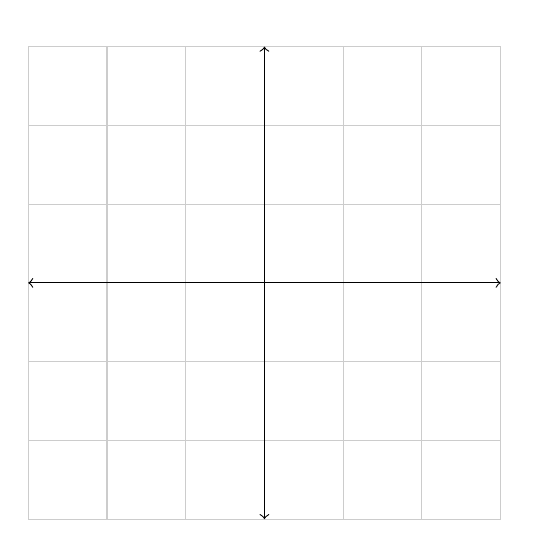
\begin{tikzpicture}
        \draw[thin,gray!40] (-3,-3) grid (3,3);
        \draw[<->] (-3,0)--(3,0) node[right]{$\RE$};
        \draw[<->] (0,-3)--(0,3) node[above]{$\IM$};
        \end{tikzpicture}
        \end{center}
        
        So, for example, let us plot a few points in the complex plane. We'll take
        \[
        z_1=1+i \qquad z_2=-1+i \qquad z_3=2-2i \qquad z_4=-2-i
        \]
        
        \begin{center}
        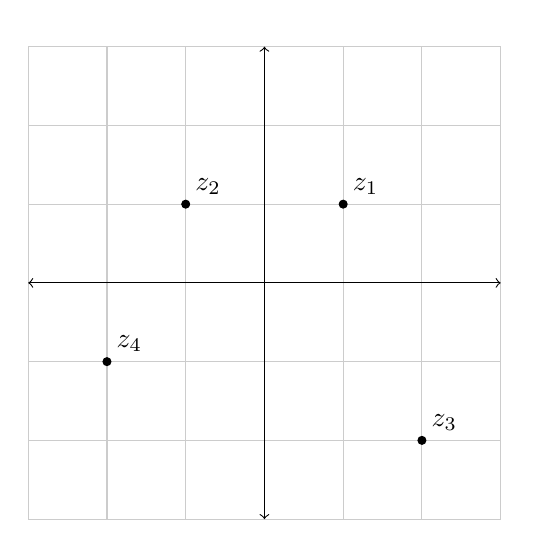
\begin{tikzpicture}
        \draw[thin,gray!40] (-3,-3) grid (3,3);
        \draw[<->] (-3,0)--(3,0) node[right]{$\RE$};
        \draw[<->] (0,-3)--(0,3) node[above]{$\IM$};
       %\addplot+[only marks] coordinates {(1,1) (-1,1) (2,-2) (-2,-1)};
        \foreach \Point/\PointLabel in {(1,1)/z_1, (-1,1)/z_2, (2,-2)/z_3, (-2,-1)/z_4}
        \draw[fill=black] \Point circle (0.05) node[above right] {$\PointLabel$};
        \end{tikzpicture}
        \end{center}
        
        \noindent Let us investigate what our algebra was doing geometrically!\\
        
        \noindent\boldgreen{Addition of complex numbers:} Recall that if we have $z_1=a_1+b_1 i$ and $z_2=a_2+b_2 i$ then
        \[
        z_1+z_2 = a_1+a_2 + (b_1 +b_2)i.
        \]
        With an explicit example, let us take
        \[
        z_1 = 1+i \qquad z_2=1-2i
        \]
        Then
        \[
        z_3=z_1+z_2=2-i.
        \]
        We can plot these in the complex plane like so.
        \begin{center}
        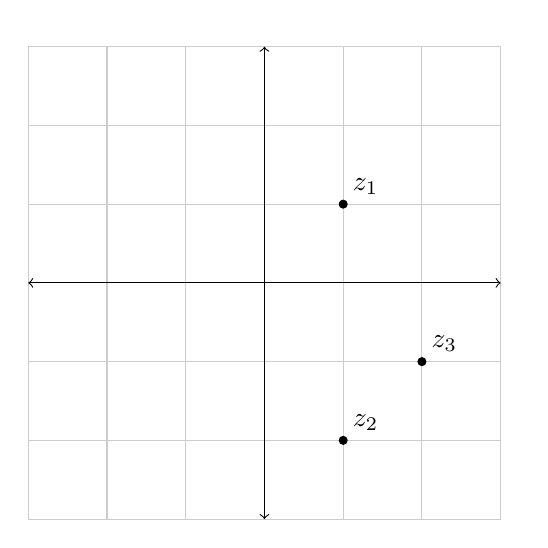
\begin{tikzpicture}
        \draw[thin,gray!40] (-3,-3) grid (3,3);
        \draw[<->] (-3,0)--(3,0) node[right]{$\RE$};
        \draw[<->] (0,-3)--(0,3) node[above]{$\IM$};
       %\addplot+[only marks] coordinates {(1,1) (-1,1) (2,-2) (-2,-1)};
        \foreach \Point/\PointLabel in {(1,1)/z_1, (1,-2)/z_2, (2,-1)/z_3}
        \draw[fill=black] \Point circle (0.05) node[above right] {$\PointLabel$};
        \end{tikzpicture}
        \end{center}   
        The other way of thinking about this addition is to think of attaching arrows to each other.  If we draw an arrow from the \emph{origin} $z=0$ to our desired point $z_i$, we can then use these arrows to perform addition.  If we take a copy of the arrow from the origin to $z_2$ and glue it to the head of the arrow from the origin to $z_1$ we arrive at our point $z_3$.
        \begin{center}
        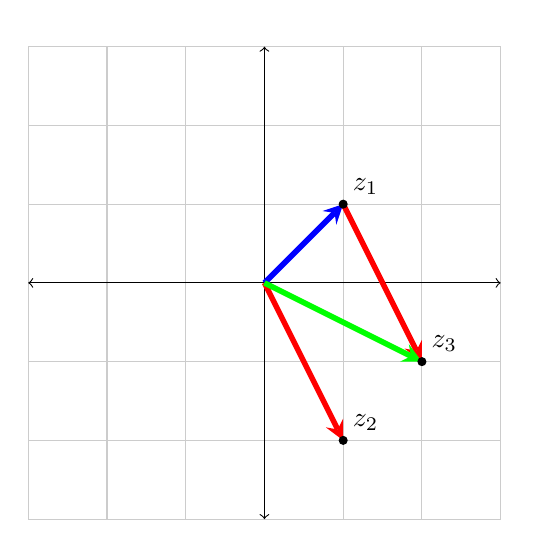
\begin{tikzpicture}
        \draw[thin,gray!40] (-3,-3) grid (3,3);
        \draw[<->] (-3,0)--(3,0) node[right]{$\RE$};
        \draw[<->] (0,-3)--(0,3) node[above]{$\IM$};
        \draw[line width=2pt,blue,-stealth](0,0)--(1,1) node[anchor=east] at (1,1){};
        \draw[line width=2pt,red,-stealth](0,0)--(1,-2) node[anchor=east] at (1,-2){};
        \draw[line width=2pt,red,-stealth](1,1)--(2,-1) node[anchor=east] at (2,-1){};
        \draw[line width=2pt,green,-stealth](0,0)--(2,-1) node[anchor=east] at (2,-1){};
        \foreach \Point/\PointLabel in {(1,1)/z_1, (1,-2)/z_2, (2,-1)/z_3}
        \draw[fill=black] \Point circle (0.05) node[above right] {$\PointLabel$};
        \end{tikzpicture}
        \end{center}
        
        How about the complex conjugate? What was this doing? Given a complex number $z=a+bi$, we know that $z^*=a-bi$.  So, take the example
        \[
        z=2+2i \qquad z^*=2-2i.
        \]
        \begin{center}
        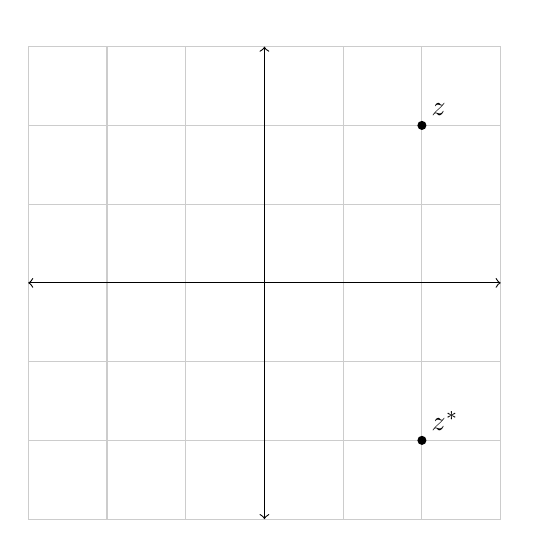
\begin{tikzpicture}
        \draw[thin,gray!40] (-3,-3) grid (3,3);
        \draw[<->] (-3,0)--(3,0) node[right]{$\RE$};
        \draw[<->] (0,-3)--(0,3) node[above]{$\IM$};
       %\addplot+[only marks] coordinates {(1,1) (-1,1) (2,-2) (-2,-1)};
        \foreach \Point/\PointLabel in {(2,2)/z, (2,-2)/z^*}
        \draw[fill=black] \Point circle (0.05) node[above right] {$\PointLabel$};
        \end{tikzpicture}
        \end{center}
        Notice that complex conjugation is just reflection about the real axis!  
        
        \section{Polar coordinates}
        An extremely important notion in planar geometry is that of \emph{polar coordinates}. Usually, we are happy to reference a point in the plane by giving the $x$-coordinates and $y$-coordinates.  In the complex case, we can give the $\RE$ and $\IM$ parts of the complex number to specify its location in the complex plane $\C$.
        
        There are many different ways you could choose to represent points in the plane, but almost all of them are rather silly to a human.  However, one that provides a great bit of intuition is polar coordinates. The idea is as follows:
        
        \begin{df}{Polar Coordinates}{pol_coord_df}
        \boldgreen{Polar coordinates}\index{polar coordinates} are the a coordinate system that uses $r$, the distance from the origin, and $\theta$, the counter-clockwise angle measured from the $\RE$ axis in the complex plane $\C$ (or $x$-axis in $\R^2$).
        \end{df}
        
        The following image may prove to be helpful.  
        
        \begin{center}
  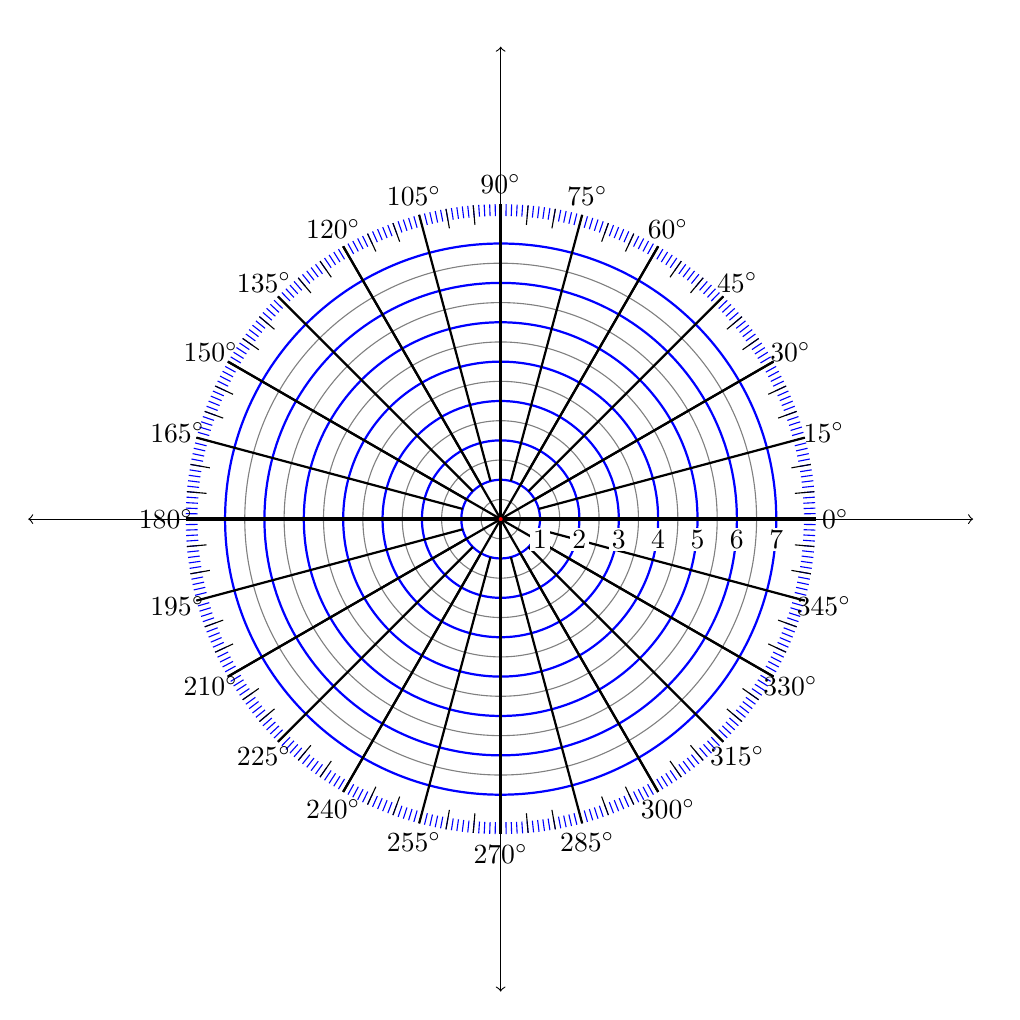
\begin{tikzpicture}[scale = .5]
        \draw[<->] (-12,0)--(12,0) node[right]{$\RE$};
        \draw[<->] (0,-12)--(0,12) node[above]{$\IM$};
    %Circles 
    \foreach \r in {1, 2,...,7}
      \draw[blue, thick] (0,0) circle (\r);    
    \foreach \r in {0.5, 1.5,...,7}
      \draw[gray, thin] (0,0) circle (\r);
    %1° Rays
    \foreach \a in {0, 1,...,359}
      \draw[blue] (\a:7.7) -- (\a:8);
    %5° Rays
    \foreach \a in {0, 5,...,359}
      \draw[black] (\a:7.5) -- (\a:8);      
    %15° Rays
    \foreach \a in {0, 15,...,359}
      \draw[thick,black] (\a:1) -- (\a:8); 
    %30° Rays
    \foreach \a in {0, 30,...,359}
      \draw[thick,black] (0, 0) -- (\a:8);
    %Radius labels (background filled white)
    \foreach \r in {1, 2,...,7}
      \draw (\r,0) node[inner sep=1pt,below=3pt,rectangle,fill=white] {$\r$};
    %Main rays
    \foreach \a in {0, 90,...,359}
      \draw[very thick] (0, 0) -- (\a:8);
    %Angle labels  
    \foreach \a in {0, 15,...,359}
      \draw (\a: 8.5) node {$\a^\circ$};
    %Central point
    \draw[fill=red] (0,0) circle(0.7mm);
  \end{tikzpicture}
\end{center}
In this picture you can see that coordinates are given by a distance from the origin and an angle.  Of course, we remember that we tend to prefer radians, so in this case we would have
\[
0^\circ = 0 \quad 45^\circ = \frac{\pi}{4} \quad 90^\circ = \frac{\pi}{2} \quad 180^\circ = \pi.
\]

\begin{question}
        Do you know where radians come from? Why are they a natural choice for angle?
\end{question}

\begin{answer}
    If we consider the unit circle (a circle with radius one), then its circumference is $2\pi$. Thus, the ``angle" around the unit circle you travel can just be given by the amount of the circumference you have traveled around.
\end{answer}

\begin{exercise}
Identify all the degrees on the above figure with their values in radians.
\end{exercise}

\begin{question}
        If we are given a point in cartesian coordinates (specifying a $\RE$ and $\IM$ part in $\C$ (or $(x,y)$ in $\R^2$), how can we find the polar coordinates $(r, \theta)$? How about vice-versa?
\end{question}
        
        \begin{answer}
            Coming to you now!
        \end{answer}
        
        \subsection{Euler's Formula}
        
        \subsubsection{Taylor Series*}
        This is a brief interlude on something we will get to later in this class.  \emph{Taylor series} are necessary for the \emph{Euler's formula}. Right now I'm just writing it so that I avoid lying to you! Fundamentally, functions we care about can be approximated by their derivatives at a single point. For example, take the function $e^x$.  It turns out, we can write this function in a new way.  That is in the form of a \emph{power series}. In fact, we have 
        \[
        e^x = \sum_{n=0}^\infty \frac{x^n}{n!}.
        \]
        More generally, for other functions (with some sufficient conditions I don't care to get into) we can write:
        \[
        f(x)=\sum_{n=0}^\infty \frac{f^{(n)}(c)}{n!}(x-c)^n.
        \]
        The latter is known as the \emph{Taylor series for $f$ centered at $x=c$}. You really may wonder why in the world I've just introduced this rather abstract concept, but it plays a fundamental role in the complex world.
        
        Using the above Taylor series for $e^x$, we can plug in the following:
        \[
        e^{i\theta}=\sum_{n=0}^\infty \frac{(i\theta)^n}{n!}.
        \]
        It turns out that we find
        \[
        e^{i\theta} = \cos \theta + i \sin \theta.
        \]
        This result is known as \boldgreen{Euler's formula}\index{Euler's formula}. We will do the rest of the work later! Just believe me for now.
        
        It turns out that Euler's formula gives us all the necessary tools to represent numbers in the complex plane in a cartesian or polar way.  So let's do a bit of work to reach this conclusion.
        
        \begin{df}{Modulus}{modulus}
        Given a complex number $z$, the \boldgreen{modulus}\index{modulus} $\|z\|$ (think \emph{length}) of a complex number is given by
        \[
        \|z\|=\sqrt{zz^*}.
        \]
        Letting $z=a+bi$ we find
        \[
        \|z\|=\sqrt{a^2+b^2},
        \]
        which is not entirely shocking.  Just like the lengths of vectors in the plane, the ``length" of a complex number follows suit.
        \end{df}
        
        \begin{question}
                Given any $\theta$, what is the modulus of $z=e^{i\theta}$?
        \end{question}
        
        \begin{answer}
        We take
        \[
        z=e^{i\theta}=\cos \theta + i \sin \theta.
        \]
        Then
        \[
        zz^*=\cos^2 \theta + \sin^2 \theta = 1.
        \]
        So
        \[
        \|z\|=\sqrt{1}=1.
        \]
        \end{answer}
        
        It turns out that there is a fundamental relationship underlying the complex numbers.  The moral of the story is that imaginary parts of complex numbers cause rotations while the real parts cause scaling. This isn't entirely the case, but it's an alright analogy. We'll be able to uncover this as we explore polar coordinates in more depth.
        
        \begin{remark}
        Something should be said here about the idea of coordinates in general.  Points in a plane are just that -- points.  Where they are located relative to each other is the fundamental structure whereas how we choose to measure this distance is not.  
        
        Polar coordinates are just another way of specifying where a point is located.  This choice of coordinates should not change the behavior of the algebra we have developed or any of the geometry.  Does choosing to measure an object in inches versus centimeters change the length of the object? Of course not.
        \end{remark}
        
        \subsection{Polar Coordinates and Transformations}
        The fact that we can write
        \[
        e^{i\theta}= \cos \theta + i \sin \theta
        \]
        means that we can control the angle of a line that the complex number lives on.  Since the above function lies on the unit circle in $\C$, we can scale this with a real number to reach any point in $\C$. This motivates the following.
        
        \begin{df}{Polar Coordinates}{pol_coord}
        An equivalent way to represent a point in $\C$ is to specify its \boldgreen{argument}\index{argument} (angle, denoted $\arg(z)$) $\theta$ and its \boldgreen{modulus}\index{modulus} (distance from the origin, denoted $r$ or $\|z\|$) $r$ and write
        \[
        z=re^{i\theta}.
        \]
        We call this coordinate representation \boldgreen{polar coordinates}. 
        \end{df}
        
        Before, we had always written this in a cartesian way, like
        \[
        z=a+bi.
        \]
        But we also have Euler's formula, which means that
        \[
        a+bi = re^{i\theta} = r\cos \theta + i r \sin \theta.
        \]
        This means that
        \[
        a=r\cos \theta
        \]
        and 
        \[
        b = r \sin \theta.
        \]
        You can also see that this is really nothing more than the Pythagorean theorem.
        
        \begin{exercise}
            Pick a point $z$ in the complex plane. Construct a right triangle where the hypotenuse goes from $0$ to $z$ and the other two sides run parallel to the $\RE$ and $\IM$ axes. Can you find $r$ and $\theta$ from this drawing? (\emph{Hint: you will need to use facts from the trigonometry section in the introduction.})
        \end{exercise}
        
        
        
        \noindent \textbf{\textbf{Conversion from polar to cartesian:}} If you're given a point in $\C$ in polar coordinates,
        \[
        z=re^{i\theta},
        \]
        then in cartesian coordinates it will read
        \[
        z=r\cos \theta + ir\sin \theta.
        \]
        This is
        \[
        a=r\cos \theta \qquad b=r\sin \theta.
        \]
        
        \noindent \textbf{\textbf{Conversion from cartesian to polar:}} If you're given a point in $\C$ is cartesian coordinates,
        \[
        z=a+bi,
        \]
        then in polar coordinates it will read
        \[
        z=\|z\|e^{i\arctan(b/a)},
        \]
        when we have $a>0$. When we have $a<0$ then we have
        \[
        z=-\|z\|e^{i\arctan(b/a)}=\|z\|e^{i(\arctan(b/a)+\pi)}.
        \]
        That is that the modulus and argument follow
        \[
        r = \|z\|=\sqrt{zz^*} \qquad \theta = \arctan\left( \frac{b}{a}\right)
        \]
        when $a>0$ and again we have
        \[
        \theta = \arctan\left(\frac{b}{a}\right)+\pi
        \]
        when $a<0$. We defined $\|z\|$ to be the distance $z$ is from the origin, so this is clear.  The $\arctan(b/a)$ can be realized from the trigonometric fact that
        \[
        \tan \theta = \frac{b}{a}
        \]
        and inverting. If we have that $a=0$, then $\theta=\frac{\pi}{2}$ or $\theta=\frac{3\pi}{2}$. Since we have
        \[
        e^{i\frac{\pi}{2}}=i \qquad \textrm{and} \qquad e^{i\frac{3\pi}{2}}=-i,
        \]
        we need only look at the sign of $b$.  If $b>0$ then $\theta=\frac{\pi}{2}$ and if $b<0$ then $\theta=\frac{3\pi}{2}$.
        
        
        \subsection{Multiplication of complex numbers in polar form}
        
        While we were perfectly happy to multiply complex numbers in Cartesian form, it is more illuminating to multiply them in polar form.  Let us take two complex numbers
        \[
        z_1 = r_1 e^{i\theta_1} \qquad z_2 = r_2 e^{i\theta_2}.
        \]
        Then we can write the product:
        \[
        z=z_1 z_2 = (r_1 e^{i\theta_1})(r_2 e^{i\theta_2})= r_1r_2 e^{i(\theta_1+\theta_2)}.
        \]
        The thing to notice here is that the modulus of a product follows
        \[
        \|z\|=\|z_1\|\|z_2\|=r_1r_2
        \]
        and the argument of a product follows
        \[
        \arg(z)=\arg(z_1)+\arg(z_2).
        \]
        All of this is to say to the following: Multiplication of complex numbers is decomposed into rotation and scaling. 
        
        \begin{center}
            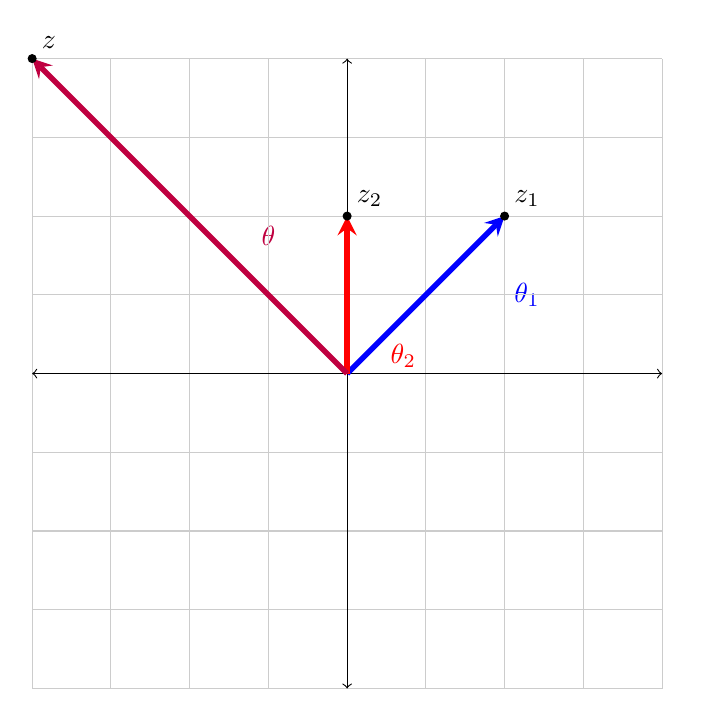
\begin{tikzpicture}
            \tdplotdrawarc[->,line width = 1pt, blue]{(0,0)}{2}{0}{45}{}{};
            \node[anchor=west] at (2,1){$\color{blue}{\theta_1}$};
            \tdplotdrawarc[->,line width = 1pt, red]{(0,0)}{1}{0}{90}{}{};
            \node[anchor=north east] at (1,.5){$\color{red}{\theta_2}$};
            \tdplotdrawarc[->,line width = 1pt, purple]{(0,0)}{1.5}{0}{135}{}{};
            \node[anchor=north] at (-1,2){$\color{purple}{\theta}$};
            \draw[thin,gray!40] (-4,-4) grid (4,4);
            \draw[<->] (-4,0)--(4,0) node[right]{$\RE$};
            \draw[<->] (0,-4)--(0,4) node[above]{$\IM$};
            \draw[line width=2pt,blue,-stealth](0,0)--(2,2) node[anchor=east] at (1,1){};
            \draw[line width=2pt,red,-stealth](0,0)--(0,2) node[anchor=east] at (2,-1){};
            \draw[line width=2pt,purple,-stealth](0,0)--(-4,4) node[anchor=east] at (2,-1){};
            \foreach \Point/\PointLabel in {(-4,4)/z, (2,2)/z_1, (0,2)/z_2}
            \draw[fill=black] \Point circle (0.05) node[above right] {$\PointLabel$};
            \end{tikzpicture}
        \end{center}
    
    
        \subsubsection{Inverse in polar form}
        We found before that given a complex number $z$, we can find the inverse $z^{-1}=1/z$ in cartesian form.  But this was a bit of a headache.  In polar form, however, it is much easier.  Recall that if we have
        \[
        z_1 z_2 = \left(r_1e^{i\theta_1}\right)\left(r_2e^{i\theta_2}\right)=r_1r_2e^{i(\theta_1+\theta_2)}.
        \]
        
        Now, given $z=re^{i\theta}$ we can find fairly quickly that $z^{-1}$ must be
        \[
        z^{-1}=\frac{1}{r}e^{-i\theta}.
        \]
        
        \begin{exercise}
        Show that this is indeed the inverse. (\emph{Hint: take our example $z^{-1}$ and multiply it by $z=re^{i\theta}$ and see that you get one.})
        \end{exercise}
        
        \section{Periodic Motion}
        
        One of the greatest benefits to complex numbers is the ability to naturally capture rotations.  When we wrote complex numbers in polar form, the rotation action became more clear. This ability makes complex numbers very useful in systems that rotate, oscillate, or have some kind of \emph{periodic} motion.
        
        \begin{question}
                What is periodic motion?
        \end{question}
        
        \begin{answer}
            Periodic motion is when a system undergoes a change that repeats itself.  For example, a mass attached to a spring will vibrate back and forth.  As the mass moves from one side to the other, it eventually gets back to where it started and repeats the process again (with no friction, of course).
        \end{answer}
        
        \noindent There is a great example of periodic motion in the complex numbers that we should take a look at.  
        
        \begin{ex}{Circular Motion}{circ_motion}
            Let us consider the function $f\colon \R \to \C$ given by
            \[
            f(t)=e^{it}.
            \]
            What happens as $t$ increases? Let's let $0<t_1<t_2<t_3<t_4<2\pi$ for now and we can plot this
            \begin{center}
            \begin{tikzpicture}
            \tdplotdrawarc[->,line width = 1pt, black]{(0,0)}{3}{0}{45}{}{};
            \node[anchor=west] at (2.75,1.25){${t_1}$};
            \tdplotdrawarc[->,line width = 1pt, black]{(0,0)}{2.25}{0}{90}{}{};
            \node[anchor=north east] at (1.5,2.5){${t_2}$};
            \tdplotdrawarc[->,line width = 1pt, black]{(0,0)}{1.5}{0}{180}{}{};
            \node[anchor=south east] at (-1,1){${t_3}$};
            \tdplotdrawarc[->,line width = 1pt, black]{(0,0)}{1}{0}{270}{}{};
            \node[anchor=north east] at (-.6,-.6){${t_4}$};
            \draw[<->] (-5,0)--(5,0) node[right]{$\RE$};
            \draw[<->] (0,-5)--(0,5) node[above]{$\IM$};
            \draw[line width=2pt,black,-stealth](0,0)--(0,4) node[anchor=south east] at (0,4){$f(t_2)$};
            \draw[line width=2pt,black,-stealth](0,0)--(2.828,2.828) node[anchor=south east] at (2.828,2.828){$f(t_1)$};
            \draw[line width=2pt,black,-stealth](0,0)--(-4,0) node[anchor=south] at (-4,0){$f(t_3)$};
            \draw[line width=2pt,black,-stealth](0,0)--(0,-4) node[anchor=east] at (0,-4){$f(t_4)$};
            % \foreach \Point/\PointLabel in {(-4,4)/z, (2,2)/z_1, (0,2)/z_2}
            % \draw[fill=black] \Point circle (0.05) node[above right] {$\PointLabel$};
            \end{tikzpicture}
        \end{center}
        Notice that by choosing $t$ in this way we have that $t$ corresponds to the angle of rotation $\theta$. 
        \end{ex}
        
        \begin{question}
            What happens when we let $t>2\pi$? 
        \end{question}
        
        \begin{answer}
            We come back around the circle. For example, if we take $\theta=\frac{\pi}{4}$ and $\Theta=2\pi + \frac{\pi}{4}$ and plug these values in to $e^{it}$ then we find:
            \begin{center}
            \begin{tikzpicture}
            \tdplotdrawarc[->,line width = 1pt, black]{(0,0)}{2}{45}{405}{}{};
            \node[anchor=west] at (0,2.25){$2\pi$};
            \tdplotdrawarc[->,line width = 1pt, black]{(0,0)}{3}{0}{45}{}{};
            \node[anchor=west] at (2.75,1.25){$\theta$};
            \draw[<->] (-3,0)--(5,0) node[right]{$\RE$};
            \draw[<->] (0,-3)--(0,5) node[above]{$\IM$};
            \draw[line width=2pt,black,-stealth](0,0)--(2.828,2.828) node[anchor=south east] at (2.828,2.828){${e^{i\theta}=e^{i\Theta}}$};
            % \foreach \Point/\PointLabel in {(-4,4)/z, (2,2)/z_1, (0,2)/z_2}
            % \draw[fill=black] \Point circle (0.05) node[above right] {$\PointLabel$};
            \end{tikzpicture}
        \end{center}
        We can see that if we add $2\pi$ to any angle $\theta$ we get back to the original angle.  
        \end{answer}
        
        \begin{df}{Periodic Function}{periodic_func}
            A function $f$ with real inputs is \boldgreen{periodic}\index{periodic} with period $T$ if 
            \[
            f(x)=f(x+T)
            \]
            for all $x$.
        \end{df}
        
        \begin{exercise}
        Realize the function $f\colon \R \to \C$ given by
        \[
        f(t)=e^{it}
        \]
        as periodic with period $2\pi$.
        \end{exercise}
        
        \begin{exercise}
        Can you name two more periodic functions with period $2\pi$? 
        \end{exercise}
        
        \begin{exercise}
        Show that the function 
        \[
        g(t)=e^{i\frac{2\pi t}{T}}
        \]
        is periodic with period $T$.
        \end{exercise}
        
        \begin{df}{Frequency}{freq}
        Let $f$ be a periodic function with period $T$. Then its \boldgreen{frequency}\index{frequency} is
        \[
        \nu = \frac{1}{T}.
        \]
        \end{df}
        
        \newpage
        
        \section{Problems}
        
        \begin{problem}
        Complete the exercises throughout the chapter.
        \end{problem}
        
        \begin{problem}
        ... To come.
        \end{problem}

\chapter{First and Second Order Dynamics}
        Roughly stated, differential equations is the study of a system that undergoes change.  This change can depend on time, space, or both.  The history of differential equations begins with Newton's study of classical mechanics.  Newton was investigating the motion of objects in space and derived the first examples of differential equations.  The field quickly grew with the once other scientists noticed the wide scope of applicability of differential equations.  
        
        In the time of Newton's classical mechanics, we saw the advent of celestial, fluid, and continuum mechanics. Examples include the diffusion, advection, and wave equations.  Other fields of science began to use these ideas from physics to model population dynamics and chemical reaction.  As time moved forward, more complicated physical interactions brought even more uses of differential equations to the forefront.  These were the dyanamical theories of electromagnetism and thermodynamics.  All of this happened before the turn of the 20$^\textrm{th}$ century.
        
        As we moved into the 1900s, there was the boom of modern physics with work from Einstein and many other scientists.  Einstein described the motion of atoms in a probabilistic manner that was also deeply related to differential equations of classical mechanics.  Soon after, he then  considered how spacetime itself behaves as a coupled dynamical continuum, much like the head of a drum that vibrates.  It was shortly after this discovery that Sch\"odinger and Heisenberg independently developed the theories of quantum mechanics.  Both stated the problem in different (but equivalent) ways.  This study brought together the notion of motion of particles with that of waves.
        
        Time passed, and in the mid 1900s computers were developed.  This forever changed the study of differential equations.  The problem was, we were finding that (other than very specific nice examples) most differential equations were extremely hard to solve.  In fact, many are so wild that the dynamics we see is volatile to the point of the so called ``butterfly effect."  These volatile systems are known as chaotic and are abundant in nature.  Weather, population, and chemical reaction are all areas where chaos can show up.  However, the ability to approximate solutions with computers allows us to make reasonable predictions and essentially solve problems that were previously deemed impossible.
        
        The goal for us is not to learn to solve many differential equations with a handbook of techniques.  These techniques can be readily found online and are very formulaic.  If you do them once, you can do them again.  Instead, our goal is to understand what differential equations model and what they say about systems.  Of course, we will explicitly solve some and see a few techniques, but that is not the emphasis.  If one pursues mathematical modelling, one will almost surely be working with computers to solve problems rather than by hand. It is with this mentality that we carry on to uncovering this structure of differential equations.
        
        \section{Ordinary Differential Equations}
        
        The first stop on the study of differential equations are the Ordinary Differential Equations \index{ordinary differential equation} (ODEs).  ODEs are equations that involve a single variable $t$ that we usually think of as time, a function $x(t)$, and derivatives of the function $x'(t)$, $x''(t)$, $x'''(t)$, up to $n$ derivatives $x^{(n)}(t)$.  We will not worry ourselves with the higher order equations yet.
        
        Unlike previous problems where we solve for a variable, or compute derivatives, we wish to find a function that satisfies the differential equation.  So, our aim is to find $x(t)$ given our understanding of how $x$ changes over time.
        
        \begin{ex}{First Order ODE}{first_order}
        Suppose we are asked to find a function $x(t)$ that satisfies the following Ordinary Differential Equation (ODE):
        \[
        x'(t) = f(t,x(t)),
        \]
        or with reduced notation
        \[
        x'=f(t,x).
        \]
        This is an example of the most general \emph{first order} ODE. 
        \begin{itemize}
            \item Written in English, this equation says, ``what function $x(t)$ has a derivative that is equal to a function of $t$ and $x(t)$?"
            \item The function $f(t,x)$ is a function of two variables. 
        \end{itemize}
        \end{ex}
        
        \noindent Often we will suppress some notation and let $x(t)$ be denoted by $x$.  We cannot forget that $x$ is a function of $t$, but it will be notationally more convenient to make this substitution. We should also say what a function of two variables is briefly.
        
        For example, we can take a function $f(t,x)$ and specify what it does with input values $t$ and $x$ simultaneously. A specific example could be
        \[
        f(t,x)=tx,
        \]
        or
        \[
        g(t,x)= t\sin\left(x^2\right),
        \]
        or
        \[
        h(t,x)= e^{t}\sqrt{x^2+tx+t^2}.
        \]
        
        \begin{exercise}
        Write your own function $p(t,x)$.
        \end{exercise}
        
        \begin{df}{Order of an ODE}{order}
        The \boldgreen{order} \index{order!differential equation} of an ODE is the highest derivative that appears in the ODE.
        \end{df}
        
        \noindent Though right now we will not investigate higher order ODEs, we should at least know what order means.  Keep this in mind as we progress.  It turns out (though we don't necessarily get to it in this course) that higher order ODEs will be equivalent to many first order ODEs.  
        
        \begin{ex}{Exponential Growth and Decay}{exp_growth_decay}
        As opposed to a very general set up, let us consider the following problem statement.\\
        
        \emph{The concentration of Plutonium in a vessel is measured over time.  It's found that the rate of change of this concentration is proportional to the current concentration.  What ODE models this situation?}\\
        
        The answer to the above question is
        \[
        x'=kx.
        \]
        \begin{itemize}
            \item We let $x(t)$ represent the concentration of Plutonium at time $t$.
            \item The rate of change of $x$, $x'(t)$, is related to the current concentration $x$ by a proportion $k$.
        \end{itemize}
        \end{ex}
        
        We like to choose our variable names in order to best communicate information.  In some cases, $x$ is not the best function name and $t$ is not the best variable name.  Try to understand the role of notation along the way.  One may see equations written differently in specific contexts. Take a look at the next example. 
        
        \begin{ex}{Mechanical Law}{mechanical_law}
        Newton's study of the motion of bodies brought him to say the following.\\
        
        \emph{The change in velocity of a body is proportional to the force applied divided by the inertial mass of the body.}\\
        
        The equation that models this is
        \[
        v'(t)=\frac{1}{m} F(t).
        \]
        \begin{itemize}
            \item The $v$ represents the body's velocity at the time $t$ and thus $v'$ is the change in velocity.
            \item The change in velocity should be equal to the applied force, $F(t)$ but also dependent on the objects mass $m$.
            \item We could also describe this equation by noting the fact that $v$ is the derivative of the position $x$. This gives
            \[
            x''(t)=\frac{1}{m}F(t).
            \]
            In other words, this is
            \[
            ma=F.
            \]
        \end{itemize}
        \end{ex}
        
        \begin{ex}{Harmonic Motion}{harmonic_motion}\index{harmonic motion}
        There are many systems that are not first order.  For example, we might have the following.\\
        
        \emph{A spring has a rest length $L$. The force on a mass on a spring is proportional to the displacement from this rest length $L$ in the direction opposite the displacement. The force causes an acceleration proportional to the force applied dived by the inertial mass of the body.}\\
        
        The governing ODE is
        \[
        y''(t) = -\frac{k}{m}(y(t)-L).
        \]
        The variable $y$ was chosen here as this equation can be written in a more standard form with a substitution.
        \end{ex}
        
        \section{Solutions to an ODE}
        
        What do we mean when we say that we want to ``solve an ODE?" This means we want to find a function whose derivatives satisfy our ODE.  Let us see a few examples.
        
        \begin{ex}{Exponential Growth and Decay Solution}{exp_growth_decay_solution}
        Previously, we were given the equation
        \[
        x'(t)=kx(t).
        \]
        I claim that 
        \[
        x(t)=Ae^{kt}
        \]
        is a \emph{general solution} to this ODE for any choice of $A$. 
        
        To verify this, we have to take the derivative of our claimed answer $x(t)$. We have,
        \[
        x'(t)=\frac{d}{dt}\left(Ae^{kt}\right)=Ake^{kt}=kx(t),
        \]
        so indeed $x(t)$ is a solution.
        \end{ex}
        
        \begin{ex}{Mechanical Law Solution}{mechanical_law_solution}
        Let us suppose that there is no force acting on the object.  We should all believe the object should move in a straight line.  With the condition of no force, the equation reads
        \[
        v'(t)=0.
        \]
        I claim that 
        \[
        v(t)=c,
        \]
        with $c$ a constant, is a solution to this equation. 
        
        To verify this, take
        \[
        v'(t)=\frac{d}{dt} c = 0.
        \]
        Indeed, this is a solution.  The solution is that of a straight line in space.  We can see this more easily by noting we also have the ODE
        \[
        x'(t) = v(t),
        \]
        since the rate of change of position is velocity. Again, I claim that
        \[
        x(t) = ct
        \]
        is a solution that is a straight line in space. 
        \end{ex}
        
        \begin{exercise}
        Verify that $x(t)$ above is indeed a solution to 
        \[
        x'(t)=x(t).
        \]
        Can you see how this means that a particle undergoing no force travels in a straight line?
        \end{exercise}

        
        \noindent Though we aren't solving equations yet, it is good practice to understand how to see when we have a solution.  Follow my methods in previous examples and do the following exercise.
        
        \begin{exercise} Earlier, we were given the following
        \[
        y''(t) = \frac{-k}{m} (y(t)-L).
        \]
        Show that
        \[
        y(t) = Ae^{i\sqrt{\frac{k}{m}}t}
        \]
        solves the above differential equation.
        \end{exercise}
        
        \section{General and Particular Solutions}
        In all previous examples, there were undetermined constants.  These constants appear since, fundamentally, an antiderivative is determined up to a constant.  Though not all ODE are solvable by direct integration, the constants are there due to this reason.
        
        How do we determine the constants?  It turns out we need a bit more information.  The extra information is also very intuitive and physical.  Take for example, a simplified version of the harmonic oscillator (spring-mass) system
        \[
        u''(t) = -u(t).
        \]
        Notice, we have just removed the constants.  This is always possible to do by picking the right way to measure the problem! Then I stated that the \emph{general solution} \index{general solution} to this ODE is
        \[
        u(t)=Ae^{it}.
        \]
        But, we don't know $A$, which is a complex number. Here, having written the solution this way is possibly confusing.  How is something that's oscillating really being described with complex numbers? It should be said that there are no ``complex measuring sticks" in the real world (that we know of).  So, our answer should end up being real valued in the end! It turns out, this solution is too general for what we think of as being physically real.
        
        \begin{df}{General Solution}{gen_soln}
            A \boldgreen{general solution} to an $n$th order ODE is a solution with $n$  (call these values $c_1,c_2,\dots,c_n$) undetermined constants. A general solution is in fact a whole family of solutions. That is, there is a solution for each different value of the constants $c_1$, $c_2$, $\dots$, $c_n$.
        \end{df}
        
        If we think about the situation, we have just determined the general oscillatory behavior of the system, but not the any particular \emph{trajectory} of the system. What we need to know is where we pulled the mass to at the initial time $t=0$. That is, we need
        \[
        x(0)
        \]
        but we also need to know how fast it was moving at that point 
        \[
        x'(0).
        \]
        The analogy is as follows: If one is throwing a ball, one needs to know where it is released $\mathbf{x}(0)$, and the velocity at which it is released at $\mathbf{x}(0)$ in order to know where the ball will land.
        \begin{figure}[H]
            \centering
            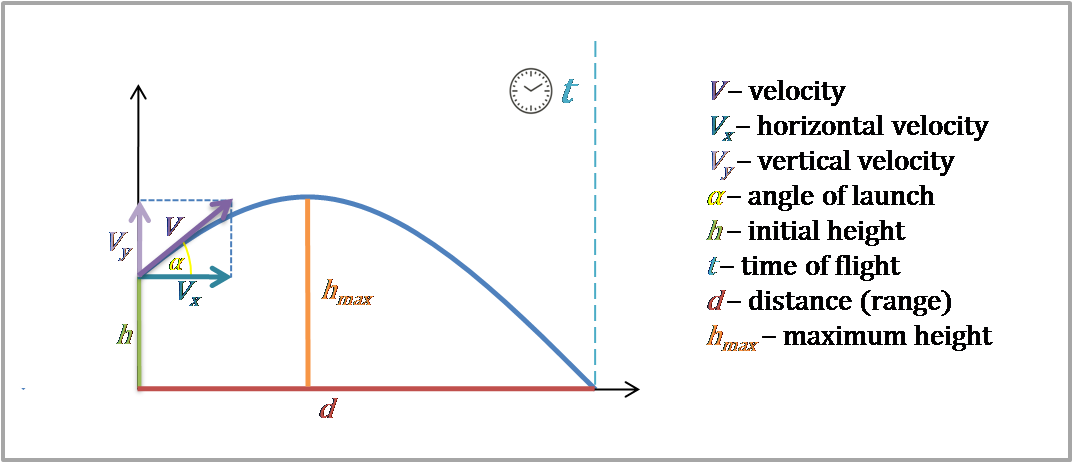
\includegraphics[width=.7\textwidth]{Figures/projectile-motion.png}
            \caption{Throwing a ball as an example of needing initial data.}
            \label{fig:proj_motion}
        \end{figure}
        \noindent We call these values $x(0)$ and $x'(0)$ the \emph{initial data}. 
        
        \begin{df}{Initial Data}{df: initial_data}
            The \boldgreen{initial data} \index{initial data} to an $n$th order ODE are the specific values for
            \[
            x(0),~ x'(0),\dots,~ x^{(n-1)}(0),
            \]
            where $x^{(k)}$ represents the $k$th derivative of $x(t)$.
        \end{df}
        
        \noindent It is from this initial data that we can figure out what a \emph{particular solution} to a problem should be.  Up to this point, we have found a general solution which is really a family of solutions. For real problems, we need one answer and not infinitely many.  
        
        \begin{df}{Particular Solution}{particular_solution}\index{particular solution}
            A \boldgreen{particular solution} is one member of the family of general solutions.  That is, a solution where the constants $c_1,~c_2,\dots,~c_n$ are all uniquely determined.
        \end{df}
        
        \noindent In other words, the particular solution is a single solution to a problem.  Specifically, we call this type of problem where we have initial data present a \boldgreen{initial value problem} \index{initial value problem}.  We will want to make note of this name as we will see \emph{boundary value problems} later on. 
        
        \begin{prop}{Initial Data and Particular Solutions}{initial_data_part_solns}
        In order to find a particular solution to an $n$th order ODE, one needs to know the initial values of the function, its derivative, its second derivative, and all derivatives up to the $(n-1)th$ derivative
        \[
        x(0),~ x'(0),\dots,~ x^{(n-1)}(0).
        \]
        \end{prop}
        
        \noindent Now, let us work through this a bit.  We can set up an initial value problem and from a general solution we can narrow in on a particular solution.  Try to keep in mind what the initial data is really meaning based on the analogy given before.
        
        
        \begin{ex}{Particular Solution to Harmonic Oscillator}{part_soln_harm_osc}
        Consider 
        \[
        u''(t)=-u(t)
        \]
        with initial data
        \[
        u(0)=1, ~ u'(0)=0.
        \]
        This has the general solution
        \[
        u(t)=Ae^{it}.
        \]
        We can find the particular solution by rewriting $x$ slightly using Euler's formula. In particular, we find
        \[
        u(t)=a\cos(t)+ib\sin(t)
        \]
        since $A$ could be any complex number.  You could also not make this substitution and find what complex number $A$ has to be.
        \[
        u(0)=a\cos(0)+ib\sin(0)=1
        \]
        from our initial data.  Specifically, this gives us that
        \[
        a=
        \]
        Then note we also have
        \[
        u'(0)=-a\sin (0) +i b\cos (0)=0
        \]
        which gives us that
        \[
        ib=0 \quad \implies \quad b=0.
        \]
        So our particular solution is
        \[
        u(t)=\cos (t).
        \]
        \end{ex}
        
        \begin{exercise}
        Plot the solution. Can you determine what is happening if we think of the oscillator as a spring mass system? What does the initial data tell us about the spring and mass at the start?
        \end{exercise}
        
        \begin{exercise}
            Instead of making the substitution using Euler's formula, solve for the complex number $A$ that shows up in $u(t)=Ae^{it}$.
        \end{exercise}
        
        The reason why we study these differential systems is to make predictions and models.  Given that, our predictions must be sensible. This means if we are given a differential equation and initial data, there should only be one particular solution.  This is known as \boldgreen{determinism}.     Not all systems are deterministic.  But it turns out the non-deterministic systems are either problematic as models or just very hard to deal with. When solving an ODE, we often call a particular solution a \boldgreen{trajectory}.
        
        \section{Separable Equations}
        The nicest possible ODEs come from equations that are \emph{separable}\index{separable differential equation}.  What this means is that, for example, we have a first order equation like
        \[
        x'=f(t)g(x).
        \]
        Why is this nice? Well, in particular, it means that we can simply integrate this equation to solve it.  Many systems exhibit symmetry that allows for this type of separation, so this technique is crucial.
        
        In general, we have
        \[
        x'=\frac{dx}{dt}
        \]
        and we put
        \begin{align*}
            \frac{dx}{dt}&=f(t)g(x)\\
            \iff \frac{dx}{g(x)} &= f(t)dt.
        \end{align*}
        With this, we can integrate both sides, then solve for $x$. That is, we compute
        \[
        \int \frac{dx}{g(x)} = \int f(t)dt,
        \]
        and we will have an equation where we can isolate $x$
        
        \begin{ex}{Separable ODE}{separable}
        Consider the following ODE where we are trying to find $x(t)$ that solves
        \[
        x'=\frac{t}{x}. 
        \]
        Then we can put
        \begin{align*}
            \frac{dx}{dt}&= \frac{t}{x}\\
            \iff xdx &= t dt.
        \end{align*}
        Then we can take the antiderivative of both sides and find
        \begin{align*}
            \int xdx &= \int t dt\\
            \iff \frac{1}{2}x^2 &= \frac{1}{2}t^2 + c\\
            \iff x&=\sqrt{t^2+2c}.
        \end{align*}
        So now we can verify that this is in fact a solution to our ODE.  So we take
        \[
        x'(t) = \frac{d}{dt}\sqrt{t^2+2c}= \frac{t}{\sqrt{t^2+2c}} = \frac{t}{x}.
        \]
        \end{ex}
        
        \begin{exercise}
        Solve the following ODE using separation
        \[
        x'(t)=t.
        \]
        Note that there will be an undetermined constant that we will learn how to handle next.
        \end{exercise}
        
        \section{Changing Variables and Symmetry}
        
        When presented with a differential equation, it can often be in a form that is not the easiest to work with.  Of course, if you do your modelling step correctly you will end up with a meaningful equation.  We want to be able to translate the correct model equation into one that is more workable.  
        
        We found that separable equations were not too bad to solve as we really just need to integrate.  Now, is it possible to turn an equation into a one that is separable? It turns out, we can when the equation satisfies a certain symmetry condition.  
        
        \begin{prop}{Reduction to Separable Equations}{reduction_separable}
            Consider the first order equation
            \[
            x'=f(x,t).
            \]
            If we have that
            \[
            f(x,t)=f(\lambda x, \lambda t)
            \]
            for any number (or function) $\lambda$, then we can reduce the equation to a separable one by defining a new variable $u=\frac{x}{t}$.
        \end{prop}
        
        The idea of changing variables is immensely important in solving real world problems.  Often times, one can gain insight on the question at hand by searching for these ``better" variables to work in.  
        
        \begin{ex}{Reduction to Separable}{reduction_separable_ex}
            Consider the differential equation
            \[
            x'=\frac{x^2+t^2}{xt}.
            \]
            We can then define
            \[
            f(x,t)=\frac{x^2+t^2}{xt}.
            \]
            Now, we can check that $f(x,t)=f(\lambda x, \lambda t)$ for any $\lambda$ by plugging in.  We have
            \begin{align*}
            f(\lambda x, \lambda t) &= \frac{(\lambda x)^2+(\lambda t)^2}{(\lambda x)(\lambda t)}\\
            &= \frac{\lambda^2(x^2+t^2)}{\lambda^2 xt}\\
            &= \frac{x^2+t^2}{xt}\\
            &=f(x,t).
            \end{align*}
            So our differential equation satisfies the necessary symmetry condition.  So, we can let $u=\frac{x}{t}$ which also means that $x=tu$ and hence
            \[
            f(x,t)=f(tu,t)=\frac{t^2u^2+t^2}{ut^2}=\frac{u^2+1}{u}.
            \]
            Note that given $x=tu$ we have $x'=u+tu'$ which we can now plug into our original expression
            \[
            x'=f(x,t)
            \]
            to get
            \[
            u+tu'=\frac{u^2+1}{u}.
            \]
            Then we can rearrange to isolate $u'$ on the right hand side
            \begin{align*}
                u+tu'&=\frac{u^2+1}{u}\\
                tu'&= \frac{u^2+1}{u}-u\\
                u'&= \frac{1}{tu}.
            \end{align*}
            This is now a separable equation! So, we can solve this in the typical way by noting we have $u'=\frac{du}{dt}$ and putting
            \[
            udu=\frac{dt}{t}.
            \]
            Then we can integrate and solve for $u$
            \begin{align*}
                \int udu &= \int \frac{dt}{t}\\
                \frac{1}{2}u^2 &= \ln(t)+c\\
                u^2&= 2\ln(t)+2c\\
                u&=\pm \sqrt{2\ln(t)+2c}.
            \end{align*}
            Recall that $u=\frac{x}{t}$ and so we have
            \begin{align*}
                \frac{x}{t}&= \pm \sqrt{2\ln(t)+2c}\\
                x&= \pm t\sqrt{2\ln(t)+2c}.
            \end{align*}
            This $x$ is our general solution to the original problem.
        \end{ex}
        
        \newpage
        
        In physical systems that conserve some quantity in time (typically energy), we will see that the differential equations assume a certain form.  This form is of an \emph{autonomous} differential equation.
        
        \begin{df}{Autonomous ODE}{autonomous_ode}
            A first order differential equation is \boldgreen{autonomous}\index{autonomous differential equation} if it can assume the form
            \[
            x'=f(x).
            \]
        \end{df}
        \noindent A first order autonomous equation is also separable. So there is not much more here to say.  They do show up quite often.
        
        Another way that symmetry can help us is more from a modelling perspective. For example, it is possible to make more clever measurements of your system! This is a much needed tool for someone keen on doing experiments. For now, do your best to follow the logic of the following substitution.  This is an example of how one can view a problem in a new way and make it easier.  We should all love symmetry like this! 
        
        \begin{ex}{Changing Variables in Harmonic Oscillator}{changing_var_harmonic}
        Consider the harmonic oscillator equation given by
        \[
        y'' = -\frac{k}{m}(y(t)-L).
        \]
        This equation, being second order, is immediately more difficult to solve.  What we can do, however, is make a change of variables to
        \[
        x(t)=y(t)-L
        \]
        and note that
        \[
        x''(t)=y''(t)
        \]
        but the ODE changes to
        \[
        x''(t)=\frac{k}{m}x(t).
        \]
        This is much easier to solve.  The idea of changing variables is extremely helpful.
        
        In these new variables, we can see the following figure.
        \begin{figure}[H]
            \centering
            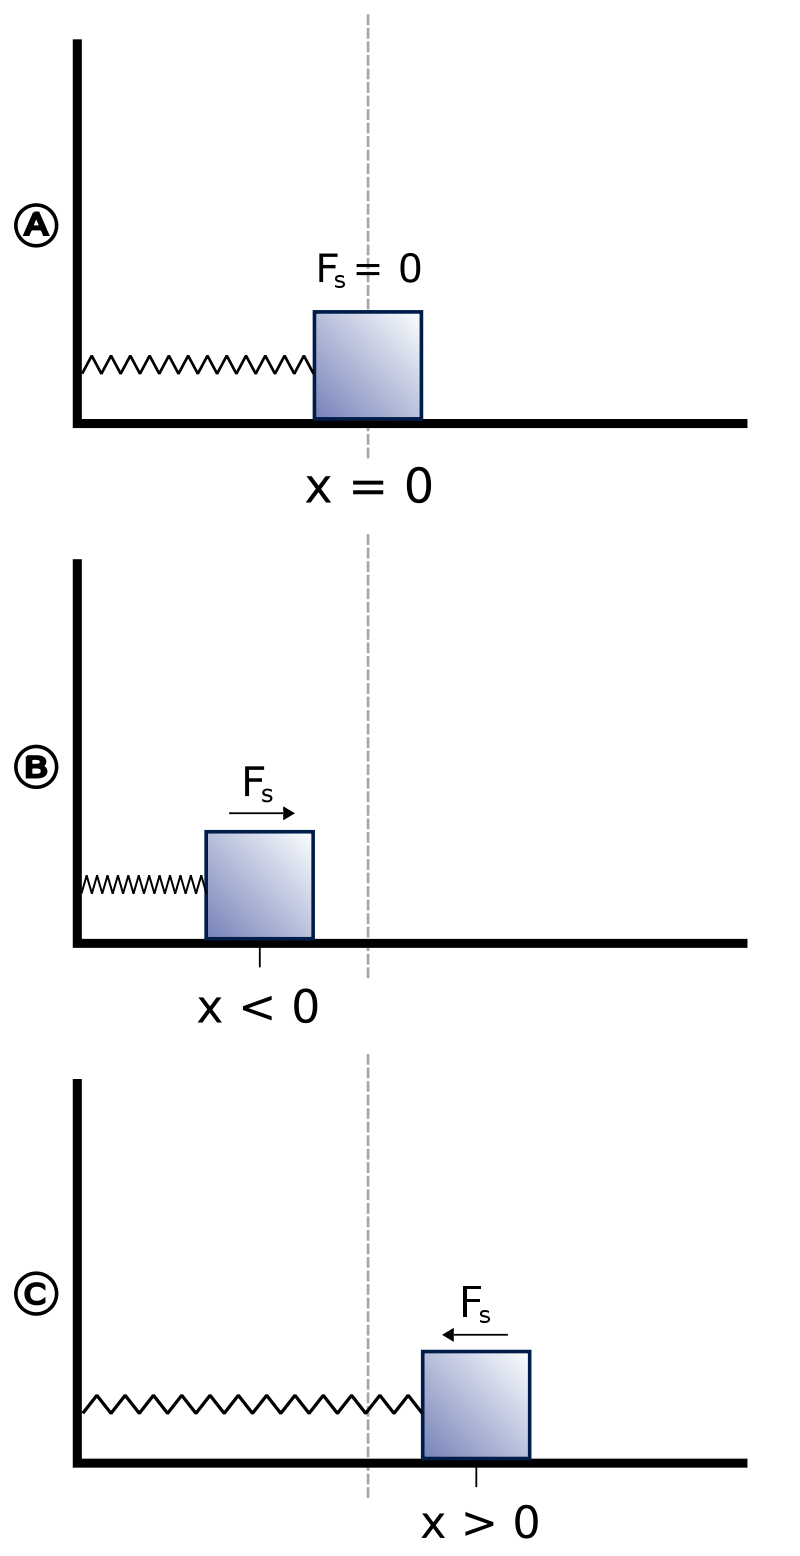
\includegraphics[width=.3\textwidth]{Figures/spring-mass.png}
            \caption{Spring-Mass system in the new variables. The dashed line represents the rest length $L$.}
            \label{fig:spring_mass}
        \end{figure}
        Interestingly enough, the rest length $L$ does not enter the new equation now. As it turns out, it is essentially a useless parameter for understanding the problem.  However, an engineer would care about changing back to our original variable $y$ as the length of a spring factors into design!
        
        How could you know to make this change? Two ways.  First, one can observe how a spring mass system oscillates.  Set up the experiment and watch for yourself, if you'd like.  What you'll see is that the mass oscillates in a symmetric way about the rest length of the spring. The experimentalist mindset will then suggest that you make the measurement about this position! The other way to observe this is as a mathematician would.  In our original expression you can notice that we have $y(t)-L$ as a quantity and that 
        \[
        \frac{d}{dt} (y(t)-L) = y'(t).
        \]
        This may be less intuitive to see, but this tells us that we can safely exchange the quantity $y(t)-L$ for a new quantity $x(t).$
        \end{ex}
        
        Earlier I claimed that this simplified equation
        \[
        x'' = -\frac{k}{m}x
        \]
        is equivalent to
        \[
        u''=-u
        \]
        by changing the units in which we measure the problem.  Indeed, consider the change of variables
        \[
        u(t)=x\left( \sqrt{k}{m}\right).
        \]
        Then 
        \[
        u'(t)=\sqrt{k}{m}x\left(\sqrt{k}{m}\right) \qquad \textrm{and} \qquad u''(t)=\frac{k}{m}x\left( \sqrt{k}{m}\right).
        \]
        
        \begin{exercise}
        Using the substitution shown above, show that the equation
        \[
        x'' = -\frac{k}{m}x
        \]
        is equivalent to
        \[
        u''=-u.
        \]
        \end{exercise}
        
        \section{First Order Linear Differential Equations}
        
        Another nice set of equations that we can solve come in the form of linear equations.  In particular, we first consider \emph{first order linear ODEs}\index{linear differential equation} but will later consider the second order version as well.  Generally, linear problems tend to be solvable whereas nonlinear problems are very hard.  One can also learn how to approximate nonlinear problems via linearization, but we do not do that here.
        
        \begin{df}{First Order Linear ODE}{first_order_lin}
            A \boldgreen{first order linear ODE} is an equation that can assume the form
            \[
            x'+f(t)x=g(t).
            \]
        \end{df}
        
        There is a general technique for solving this type of equation and, in fact, a general technique for solving higher order linear equations.  More on that later.  For now, let us work to solve this problem.  The method we will use utilizes a function called an \boldgreen{integrating factor}\index{integrating factor}. The idea is that we can use the format of the equation to our advantage.
        
        \subsubsection{Integrating Factor}
        Consider a first order linear ODE given by
        \[
        x'+f(t)x=g(t).
        \]
        Then, multiply the whole expression by a yet undetermined function $\mu(t)$ to get
        \begin{equation}
        \mu(t)x'+\mu(t)f(t)x=\mu(t)g(t). \label{eq:int_fact_1}
        \end{equation}
        The reason we have done this is that we can now take a look at the derivative of the product
        \begin{equation}
        \left( \mu(t)x\right)'= \mu'(t)x+\mu x'. \label{eq:int_fact_2}
        \end{equation}

        From here, we can set this product derivative (right hand side of \ref{eq:int_fact_2}) equals the left hand side of expression \ref{eq:int_fact_1}.  This gives us
        \[
        \mu'(t)x+\mu x' = \mu(t)x'+\mu(t) f(t) x
        \]
        which means that
        \[
        \mu'(t)x=\mu(t) f(t) x.
        \]
        This is a separable ODE! So we can solve this for $\mu$ using the separation technique. This $\mu$ is the integrating factor.
        
        \begin{exercise}
            Solve the separable ODE
            \[
            \mu'(t)x=\mu(t)f(t)x
            \]
            for $\mu$ and show that you find
            \[
            \mu(t) = e^{\int f(t)dt}.
            \]
        \end{exercise}
        
        \noindent From the exercise, we have that
        \[
        \mu(t)=e^{\int f(t)dt}
        \]
        and we can use this to complete the problem.  Specifically, we have that the left hand side of \ref{eq:int_fact_2} is equal to the right hand side of \ref{eq:int_fact_1} to get
        \[
        (\mu(t) x)' = \mu(t)g(t).
        \]
        We can integrate both sides and solve for $x$ to find
        \[
        \boxed{x = \frac{1}{\mu(t)}\int \mu(t) g(t)dt.}
        \]
        The above expression for $x$ tells us the general solution to any first order linear ODE.
        
        \begin{ex}{Solving an ODE with Integrating Factor}{solving_ode_int_fact}
            Consider the first order equation
            \[
            x'+\frac{2x}{t}=2\cos(t).
            \]
            Note that we can say $f(t)=\frac{2}{t}$ and then 
            \begin{align*}
            \mu(t)&=e^{\int \frac{2}{t}dt}\\
            &= e^{2\ln(t)}\\
            &=t^2.
            \end{align*}
            Note, when computing the integrating factor $\mu$ we do not need to have a $+c$ after integrating. It will cancel later on if you do include it. Next, we note that
            \[
            x=\frac{1}{\mu(t)} \int \mu(t) g(t)dt
            \]
            where $g(t)=2\cos(t)$ in this case.  Thus
            \begin{align*}
                x&=\frac{1}{t^2} \int t^2 \cdot 2\cos(t)dt\\
                &=\frac{2}{t^2} \left(t^2\sin(t)+2t\cos(t)-2\sin(t)+c\right),
            \end{align*}
            where the last equality involved using integration by parts twice.  So we have found a general solution to our original ODE.
        \end{ex}
        
        \begin{exercise}
            Complete the integration by parts in the above example.
        \end{exercise}
        
        Just to introduce some terminology, we can note that if we have a first order linear ODE of the form
        \[
        x'+f(t)x=0
        \]
        we call this equation \boldgreen{homogeneous}\index{homogeneous!differential equation}.  Otherwise, we have that the expression with a nonzero right hand side
        \[
        x'+ f(t)x=g(t)
        \]
        is called \boldgreen{inhomogenous}\index{inhomogeneous!differential equation}.  The homogeneous case for first order equations are simply separable equations and the distinction here is not really necessary.
        
        \section{Applications to Chemical Kinetics}
        \index{chemical kinetics}
        As a chemist, one would probably like to understand how we can model elementary chemical reactions with mathematics.  For example, maybe we would like to understand the rate of reaction of hydrogen $H_2$ and oxygen $O_2$ to create water $H_2 O$. We typically write
        \[
        2H_2 + O_2 \to 2H_2O.
        \]
        \noindent Of course, we should actually be writing
        \[
        2H_2 + O_2 \leftrightarrows 2H_2O
        \]
        since real reactions have an equilibrium.  The amount of back and forth in a reaction also depends on parameters like temperature, pressure, or concentration.
        
        For now, let us assume we are looking at the original model which can we written as a sum of $m$ reactants $R_i$ each with an amount $r_i$ that give us an amount $p_i$ of $n$ different products $P_j$. That is, we have a reaction
        \begin{align*}
            r_1R_1 + r_2R_2 + \cdots + r_mR_m \to p_1 P_1 + p_2P_2 +\cdots p_n P_n,
        \end{align*}
        that gives us an equation
        \[
        \sum_{i=1}^m r_iR_i = \sum_{j=1}^n p_jP_j.
        \]
        The second is just a mathematically succinct way of representing the quantitites in the reaction. We will call the $r_i$ and $p_j$ the \boldgreen{stoichiometric variables}. We often write the equation above in the following form:
        \begin{equation}
        0=\sum_{j=1}^n p_j P_j - \sum_{i=1}^m r_iR_i. \label{eq:stoich}
        \end{equation}
        
        Suppose we start with an initial amount of substance $A$, $N_{A0}$. Then we say that the amount of species $A$ at time $t$ is $N_{A}$.  The amount of reaction observed is given by the \boldgreen{extent of reaction} $\xi$ defined by
        \[
        N_A = N_{A0}+a\xi.
        \]
        Note that $a$ will be negative for products as the number of products decreases over time. To see this, see \ref{eq:stoich} which states that the total number of species has to be conserved. Then the \boldgreen{rate of conversion} is 
        \begin{align*}
            \rho &= \frac{d\xi}{dt}\\
            &= \frac{1}{a}\frac{dN_a}{dt}.
        \end{align*}
        
        More often than not, we care about concentrations of chemicals as opposed to amount. So we let
        \[
        [A]=\frac{N_A}{V}
        \]
        where $V$ is the volume the substance $A$ is contained in.  Then we have
        \[
        v=\frac{\rho}{V}=\frac{1}{a}\frac{d[A]}{dt}.
        \]
        Now, for a reaction 
        \[
        r_1R_1 + r_2R_2 + \cdots + r_mR_m \to p_1 P_1 + p_2P_2 +\cdots p_n P_n,
        \]
        we must have that the concentrations must change with matching rates so that
        \[
        v=-\frac{1}{r_i}\frac{d[R_i]}{dt}=\frac{1}{p_j}\frac{d[P_j]}{dt},
        \]
        for every product $P_j$ and reactant $R_i$.
        
        \begin{ex}{$H_2$ and $O_2$ to $H_2O$}{water}
        If we are wishing to model
        \[
        2H_2 + O_2 \to 2H_2O
        \]
        we will have the equations
        \begin{align*}
            v=-\frac{1}{2}\frac{d[H_2]}{dt}=-\frac{d[O_2]}{dt}=\frac{1}{2}\frac{d[H_2O]}{dt}.
        \end{align*}
        \end{ex}
        
        From experiment one can determine that
        \[
        v=k[R_1]^{\alpha_1}[R_2]^{\alpha_2}\cdots
        \]
        which allows us to complete our model.  We call $k$ the \boldgreen{rate constant} of the reaction and the numbers $\alpha_i$ dtermine that \boldgreen{order of the reaction}. We say that $\alpha_i$ is the order with respect to the reactant $R_i$. For example, we may have
        \begin{itemize}
            \item First order: $R \to \textrm{Products}$;
            \item Second order: $2R \to \textrm{Products}$;\\
            \item Second order: $R_1+R_2 \to \textrm{Products}$.
        \end{itemize}
        
        \begin{ex}{First Order Reaction}{first_order_react}
        Consider a reaction
        \[
        R \to \textrm{Products}
        \]
        with an initial concentration of $R$ given by $[R]_0$. We then have
        \[
        v=\frac{-d[R]}{dt}=k[R].
        \]
        For ease of notation, let $x=[R]$ and we have
        \[
        x'=-kx,
        \]
        which we have solved before.
        \end{ex}
        
        \begin{exercise}
        Either solve the above differential equation again, or find the solution to the initial value problem somewhere in this text.
        \end{exercise}
        
        \begin{ex}{Second Order Reaction}{second_order_react}
        Consider a reaction
        \[
        2R \to \textrm{Products}
        \]
        with an initial concentration $[R]_0$.  Then we have
        \[
        v=-\frac{1}{2} \frac{d[R]}{dt}=k[R]^2.
        \]
        Again, let $x=[R]$ and we have the ODE
        \[
        x'=-2kx^2.
        \]
        \end{ex}
        
        \begin{exercise}
        Find the particular solution to the initial value problem posed in the previous example.
        \end{exercise}
        
        
        %% THERE MAY BE MISTAKES HERE
        \begin{ex}{Several Reactions}{sev_react}
        Consider a chain of reactions as follows
        \[
        A\xrightarrow{k_1} B \xrightarrow{k_2} C.
        \]
        Then we wish to describe the concentrations of each species $A$, $B$, and $C$ over time. We know that we have
        \[
        \frac{d[A]}{dt}=-k_1[A]
        \]
        and it follows that
        \[
        \frac{d[b]}{dt}=k_1[A]-k_2[B].
        \]
        Then, at time $t=0$ we have initial concentrations $[A]_0$, $[B]_0=0$, and $[C]_0$ so that we are only starting with species $A$. Later on, at time $t$, we have $[A]=[A]-x$ and $[B]=y$ which means that we have $[C]=x-y$.  Note that $[C]$ is created by $A\to B$ and from $B\to C$ so we must subtract off the concentration of $B$ that has not converted to species $C$ yet. This gives us the equations
        \begin{equation}
                        \frac{d([A]_0-x)}{dt}=-k_1([A]-x) \label{eq:chem_a}
        \end{equation}
        \begin{equation}
                        \frac{dy}{dt}=k_1([A]_0-x)-k_2y. \label{eq:chem_b}
        \end{equation}
        Note that \ref{eq:chem_a} is a separable equation with solution
        \[
        [A]_0-x=[A]_0e^{-k_1t}.
        \]
        We can then substitute in this solution to \ref{eq:chem_b} to get
        \[
        \frac{dy}{dt}=[A]_0k_1e^{-k_1t}-k_2y
        \]
        which gives us the first order linear equation
        \[
        y'+k_2y=[A]_0k_1e^{-k_1t}.
        \]
        To solve this, we find the integrating factor
        \[
        \mu(t)=e^{\int k_2 dt}=e^{k_2t}.
        \]
        Then we have that
        \[
        y=\frac{1}{e^{k_2t}}\int e^{k_2t}[A]_0k_1e^{-k_1t}dt=[A]_0k_1e^{-k_2t}\int e^{(k_2-k_1)t}dt.
        \]
        This integral comes down to two cases; first when $k_1=k_2$ and when $k_1\neq k_2$. Thus we have
        \[
        y=\begin{cases}
        \frac{[A]_0k_1}{k_2-k_1}e^{-k_1t}+ce^{-k_2t} & k_1\neq k_2\\
        [A]_0k_1te^{-k_1t}+ce^{-k_2t} & k_1=k_2.
        \end{cases}
        \]
        Using our initial conditions, we have $y=0$ at time $t=0$ which gives us the particular solution
        \[
        y=\begin{cases}
        \frac{[A]_0k_1}{k_2-k_1}\left( e^{-k_1t}-e^{-k_2t}\right) & k_1\neq k_2\\
        [A]_0k_1te^{-k_2t} & k_1=k_2.
        \end{cases}
        \]
        
        Now, we will have that each concentration can be written as
        \begin{align*}
            [A]&=[A]_0e^{-k_1t}\\
            [B]&=\begin{cases}
        \frac{[A]_0k_1}{k_2-k_1}\left( e^{-k_1t}-e^{-k_2t}\right) & k_1\neq k_2\\
        [A]_0k_1te^{-k_2t} & k_1=k_2.
        \end{cases}\\
        [C]&=[A]_0-[A]-[B].
        \end{align*}
        Now, we can plot the concentrations below letting $[A]$ be in purple, $[B]$ in red, and $[C]$ in black.
        \begin{figure}[H]
    \centering
    \begin{subfigure}[h]{0.3\textwidth}
        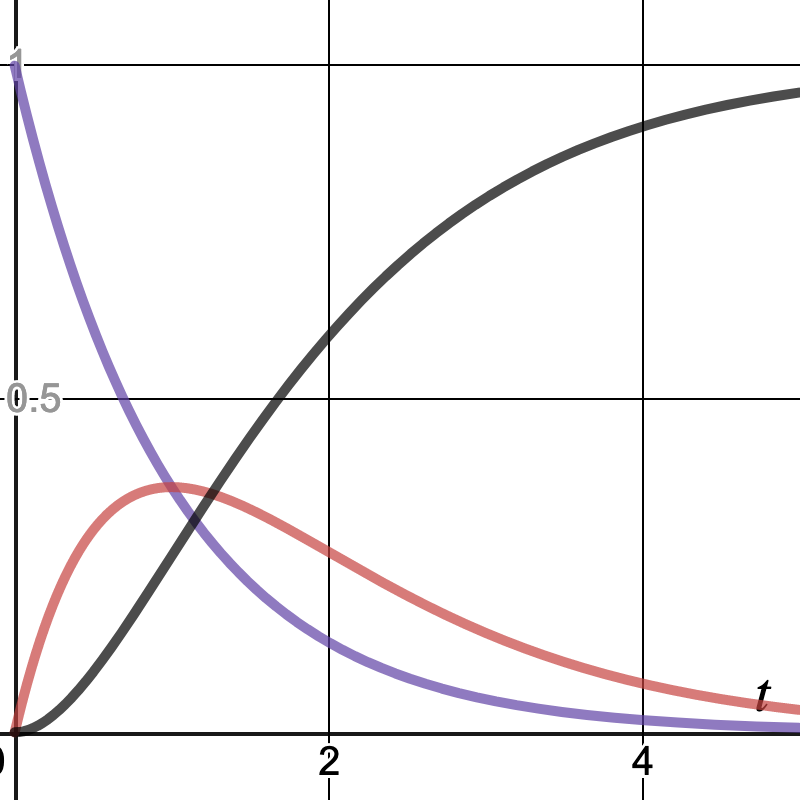
\includegraphics[width=\textwidth]{Figures_Part_2/k1=k2.png}
        \caption{$k_1=k_2=1$.}
    \end{subfigure}
    ~ 
    \begin{subfigure}[h]{0.3\textwidth}
        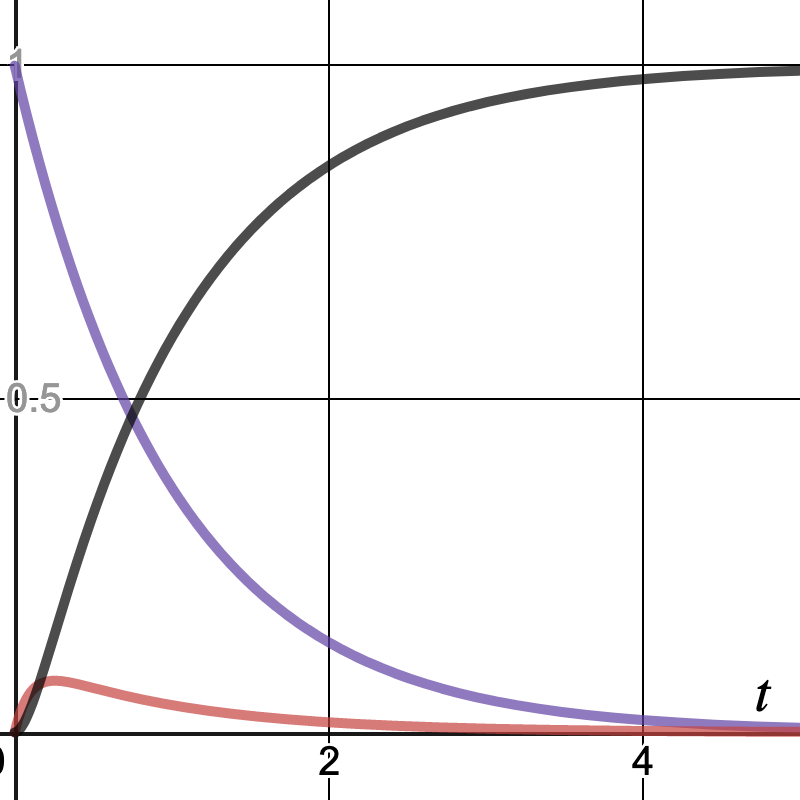
\includegraphics[width=\textwidth]{Figures_Part_2/k1=1k2=10.png}
        \caption{$k_1=1$ and $k_2=10$.}
    \end{subfigure}
    ~
    \begin{subfigure}[h]{0.3\textwidth}
        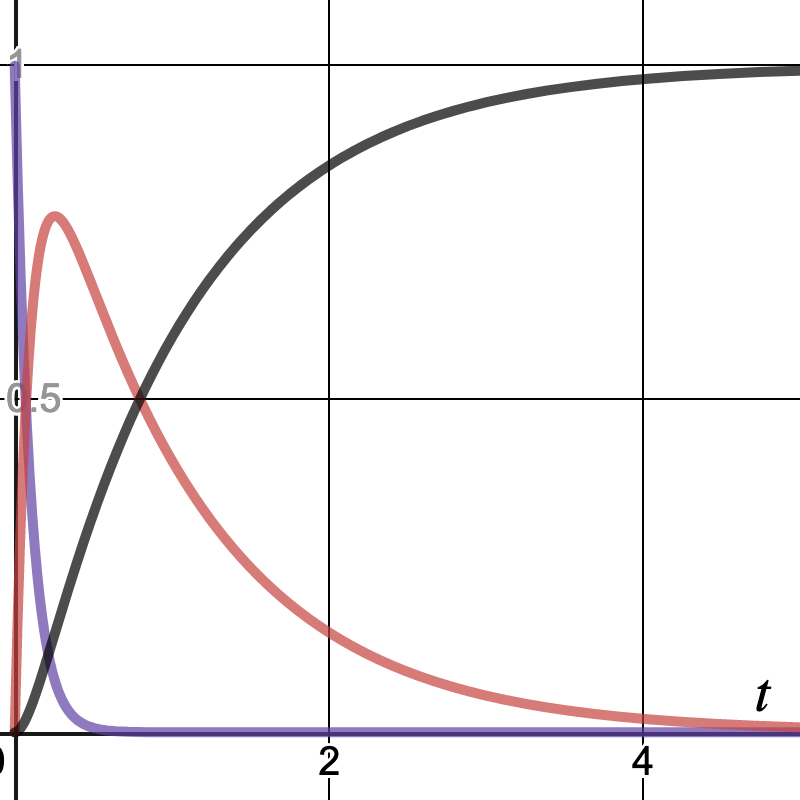
\includegraphics[width=\textwidth]{Figures_Part_2/k1=10k2=1.png}
        \caption{$k_1=10$ and $k_2=1$.}
    \end{subfigure}

        \end{figure}
        \end{ex}
        
        \begin{exercise}
        Go through the previous example and fill in the missing steps.
        \end{exercise}
        
        \section{Second Order Equations}
        
        Since Newtonian physics is governed by the equation
        \[
        F=ma=mx''
        \]
        we often see differential equations that are second order.  The question is then, how can we solve these?  
        
        There are a two main forms of second order equations we will consider, but there are more out there. Let's define the class of equations we will stick with.
        
        \begin{df}{Second Order Linear ODEs}{second_order_lin}
            A second order ODE is \boldgreen{linear}\index{linear!differential equation} if it can assume the form 
            \[
            x''+f(t)x'+g(t)x=h(t).
            \]
            We say that the equation is \boldgreen{homogeneous}\index{homogeneous!differential equation} if $h(t)=0$ and otherwise it is \boldgreen{inhomogenous}\index{inhomogeneous!differential equation}.
        \end{df}
        
        \begin{remark}
        An inhomogenous second order linear ODE \underline{can} be always be solved with the functions $f$, $g$, and $h$ are smooth enough.  We will not cover solving this general of a problem here.
        \end{remark}
        
        \subsection{Homogeneous and Constant Coefficients}
        Specifically, we care about homogeneous second order linear ODEs where the functions $f(t)=b$ and $g(t)=c$ are constant.  These will be the most simple to solve yet fairly applicable. An equation like this can be rearranged to take the form
        \[
        x''+bx'+cx=0.
        \]
        A reasonable guess (or \boldgreen{ansatz}\index{ansatz}) for a solution is an exponential function of the form
        \[
        x(t)=Ae^{\lambda t}
        \]
        where $A$ is an arbitrary constant. Since we can see that each successive derivative seems to only multiply our function by a constant, this is a good first guess. If we try to make this function $x$ work to solve our ODE, we plug it in and see that we get
        \begin{align*}
            \left(Ae^{\lambda t}\right)''+b\left(Ae^{\lambda t}\right)'+cAe^{\lambda t}&=0\\
            \iff\lambda^2 Ae^{\lambda t}+\lambda b Ae^{\lambda t} +c Ae^{\lambda t}&=0\\
            \iff Ae^{\lambda t}\left( \lambda^2 + b\lambda +c\right)&=0\\
            \iff \lambda^2 +b\lambda +c &=0.
        \end{align*}
        The last equality must be true since $Ae^{\lambda t}$ is never equal to zero.  Thus, it seems we found a solution to the equation via the roots of this polynomial
        \[
        \lambda^2+b\lambda +c,
        \]
        which we will refer to as the \boldgreen{characteristic polynomial}\index{characteristic polynomial}. The roots of the characteristic polynomial are then able to be found with the quadratic formula to yield
        \[
        \lambda=\frac{-b\pm \sqrt{b^2-4c}}{2}.
        \]
        This leads us to the following.
        
        \begin{prop}{Solutions to Linear Constant Coefficient Second Order ODE}{solutions_hom_constant}
        Given the differential equation
        \[
        x''+bx'+cx=0
        \]
        with roots of the characteristic polynomial
        \[
        \lambda^2+b\lambda +c
        \]
        equal to $\lambda_1$ and $\lambda_2$, we have the general solution:
        \[
        x(t)=C_1 e^{\lambda_1t}+C_2e^{\lambda_2t}
        \]
        where $C_1,C_2,\lambda_1,\lambda_2 \in \C$.
        \end{prop}
        
        \begin{question}
        Above we see that we have a sum of solutions and our ansatz only chose one. Is it always possible to have a sum of different solutions be a solution?
        \end{question}
        
        \begin{answer}
        Yes. We will see by the following theorem that this is the case! This is an important result for studying quantum systems.
        \end{answer}
        
        \begin{thm}{Superposition of Solutions}{superposition_solns}
        Let $x_1$ and $x_2$ be general solutions to the equation
        \[
        x''+f(t)x'+g(t)x=0.
        \]
        Then any \boldgreen{linear combination}\index{linear combination} (or \boldgreen{superposition}\index{superposition}) of solutions
        \[
        \alpha_1 x_1 + \alpha_2 x_2
        \]
        with $\alpha_1,\alpha_2\in \C$, is also a solution.\\
        
        \begin{proof}
        Let $x_1$ and $x_2$ be general solutions to the above ODE. Then consider the function
        \[
        x=\alpha_1 x_1 + \alpha_2 x_2.
        \]
        Then we have
        \begin{align*}
            x''+f(t)x'+g(t)x&= (\alpha_1 x_1 + \alpha_2 x_2)''+f(t)(\alpha_1x_1+\alpha_2 x_2)'+g(t)(\alpha_1x_1+\alpha_2x_2)\\
            &= \alpha_1 x_1'' + \alpha_2 x_2'' + \alpha_1 f(t)x'+\alpha_2 f(t)x_2'+\alpha_1 g(t)x_1 + \alpha_2 g(t) x_1\\
            &= \alpha_1 ( x_1''+f(t)x_1'+g(t)x_1)+\alpha_2(x_2''+f(t)x_2'+g(t)x_2)\\
            &=0, \quad\textrm{since $x_1$ and $x_2$ are solutions.}
        \end{align*}
        Hence $x=\alpha_1x_1 + \alpha_2 x_2$ is also a solution.
        \end{proof}
        \end{thm}
        
        \begin{remark}
        You may have heard of superposition in quantum mechanics. It turns out that this is exactly what is meant in the mathematical theory. Eventually, we'll see an example of what this physically means in a quantum system.
        \end{remark}
        
        \begin{ex}{Solving the Harmonic Oscillator}{solve_harmonic}
        Consider the equation
        \[
        mx''=-kx
        \]
        with the initial data $x(0)=1$ and $x'(0)=0$. We have shown that we have a solution to this equation before, but now we can explicitly solve it.  We can rewrite the ODE as a second order linear homogeneous equation with constant coefficients by putting
        \[
        x''+\frac{k}{m}x=0.
        \]
        Then, for sake of notation, let $\omega = \sqrt{\frac{k}{m}}$ so that
        \[
        x''+\omega^2x=0.
        \]
        Then the characteristic polynmomial is
        \[
        \lambda^2+\omega^2
        \]
        and the roots are
        \begin{align*}
            \lambda^2+\omega^2&=0\\
            \lambda^2&=-\omega^2\\
            \iff \lambda&= \pm \sqrt{-\omega^2}= \pm i \omega.
        \end{align*}
        Thus, the general solution is then
        \[
        x=C_1 e^{i\omega t}+C_2e^{-i\omega t}
        \]
        where $C_1,C_2\in \C$.
        
        Now, we can find the particular solution from the initial data $x(0)=1$ and $x'(0)=0$ and letting
        \[
        C_1=a_1+b_1i \qquad \textrm{and} \qquad C_2=a_2+b_2i.
        \]
        We then have
        \begin{align*}
                    1=x(0)&=(a_1+b_1i)e^{i\omega \cdot 0}+(a_2+b_2 i)e^{-i\omega \cdot 0}\\
                    &=(a_1+b_1i)+(a_2+b_2i)\\
                    &=(a_1+a_2)+i(b_1+b_2).
        \end{align*}
        Thus we must have 
        \begin{align*}
            a_1+a_2&=1\\
            b_1+b_2&=0 ~\implies~ b_1=-b_2.
        \end{align*}
        From the other initial condition, we have
        \begin{align*}
        0=x'(0)&=\omega(a_1+b_1i)e^{i\omega \cdot 0}-\omega (a_2+b_2i)e^{i\omega \cdot 0}\\
        &=(a_1-a_2)+i(b_1-b_2).
        \end{align*}
        Thus we have
        \begin{align*}
            a_1-a_2&=0 ~\implies~ a_1=a_2\\
            b_1-b_2&=0 ~\implies~ b_1=b_2.
        \end{align*}
        Now we have $b_1=-b_2$ and $b_1=b_2$ which means $b_1=b_2=0$.  Then, we also have $a_1=a_2$ which we can substitute into $a_1+a_2=1$ to find that $a_1=a_2=1/2$.  Hence we have our particular solution
        \begin{align*}
            x(t)&=\frac{1}{2}e^{i\omega t}+\frac{1}{2}e^{-i\omega t}.
            \end{align*}
            This, we can rewrite to find a more familiar form of the solution by
            \begin{align*}
            x(t)&= \frac{1}{2}(\cos(\omega t)+i\sin(\omega t)) + \frac{1}{2}(\cos(-\omega t)+i\sin(-\omega t))\\
            &= \frac{1}{2}(\cos(\omega t)+i\sin(\omega t))+\frac{1}{2}(\cos(\omega t)-i\sin(\omega t))
            &=\cos(\omega t).
        \end{align*}
        Note that I used the fact that sine is an odd function meaning that $\sin(-x)=-\sin(x)$ and that cosine is an even function meaning $\cos(-x)=\cos(x)$.  
        \end{ex}
        
        \newpage
        
        \begin{exercise}
        Find where we claimed a solution to the harmonic oscillator earlier in this text and check that this solution matches that.
        \end{exercise}
        
        \subsection{Qualitative Analysis}
        
        Solutions to homogeneous second order linear ODEs with constant coefficients only come in a few different classes of solutions. Essentially, they oscillate, exponentially grow or decay, or a combination of the two.  There are some edge cases to be careful of, but they are not typical.  Let's see why this is the case.
        
        Recall that we have, in general, an equation 
        \[
        x''+bx'+cx=0
        \]
        which gives rise to the characteristic polynomial
        \[
        \lambda^2+b\lambda + c.
        \]
        The roots are then
        \[
        \lambda = \frac{-b\pm \sqrt{b^2-4c}}{2}= \frac{-b}{2}\pm \frac{\sqrt{b^2-4c}}{2}.
        \]
        These roots can be real, complex, or purely imaginary. The real part can be greater than zero, or less.  These facts encompass all the solutions we care about.
        
        \begin{itemize}
            \item \textbf{Case 1:} Consider the case where the roots of the characteristic polynomial are both real and denote the roots by $\lambda_1$ and $\lambda_2$.  If this is the case, then we must have that $b^2>4c$ so that the square root in the quadratic formula is not of a negative number. For this, we have two subcases.
            \begin{itemize}
                \item \textbf{Subcase 1:} If we have two distinct real roots, $\lambda_1$ and $\lambda_2$ where $\lambda_1\neq \lambda_2$, then our general solution to the equation is
                \[
                x(t)=C_1e^{\lambda_1 t}+C_2e^{\lambda_2 t}.
                \]
                Note that $\lambda_1$ and $\lambda_2$ could be both positive, both negative, one negative one positive, or either could be zero as well.
                
                Let's say we have $\lambda_1=1$, $\lambda_2=-1$ and let $C_1=C_2=1$. Then the solution plotted in the $xt$-plane looks like
                \begin{figure}[H]
                    \centering
                    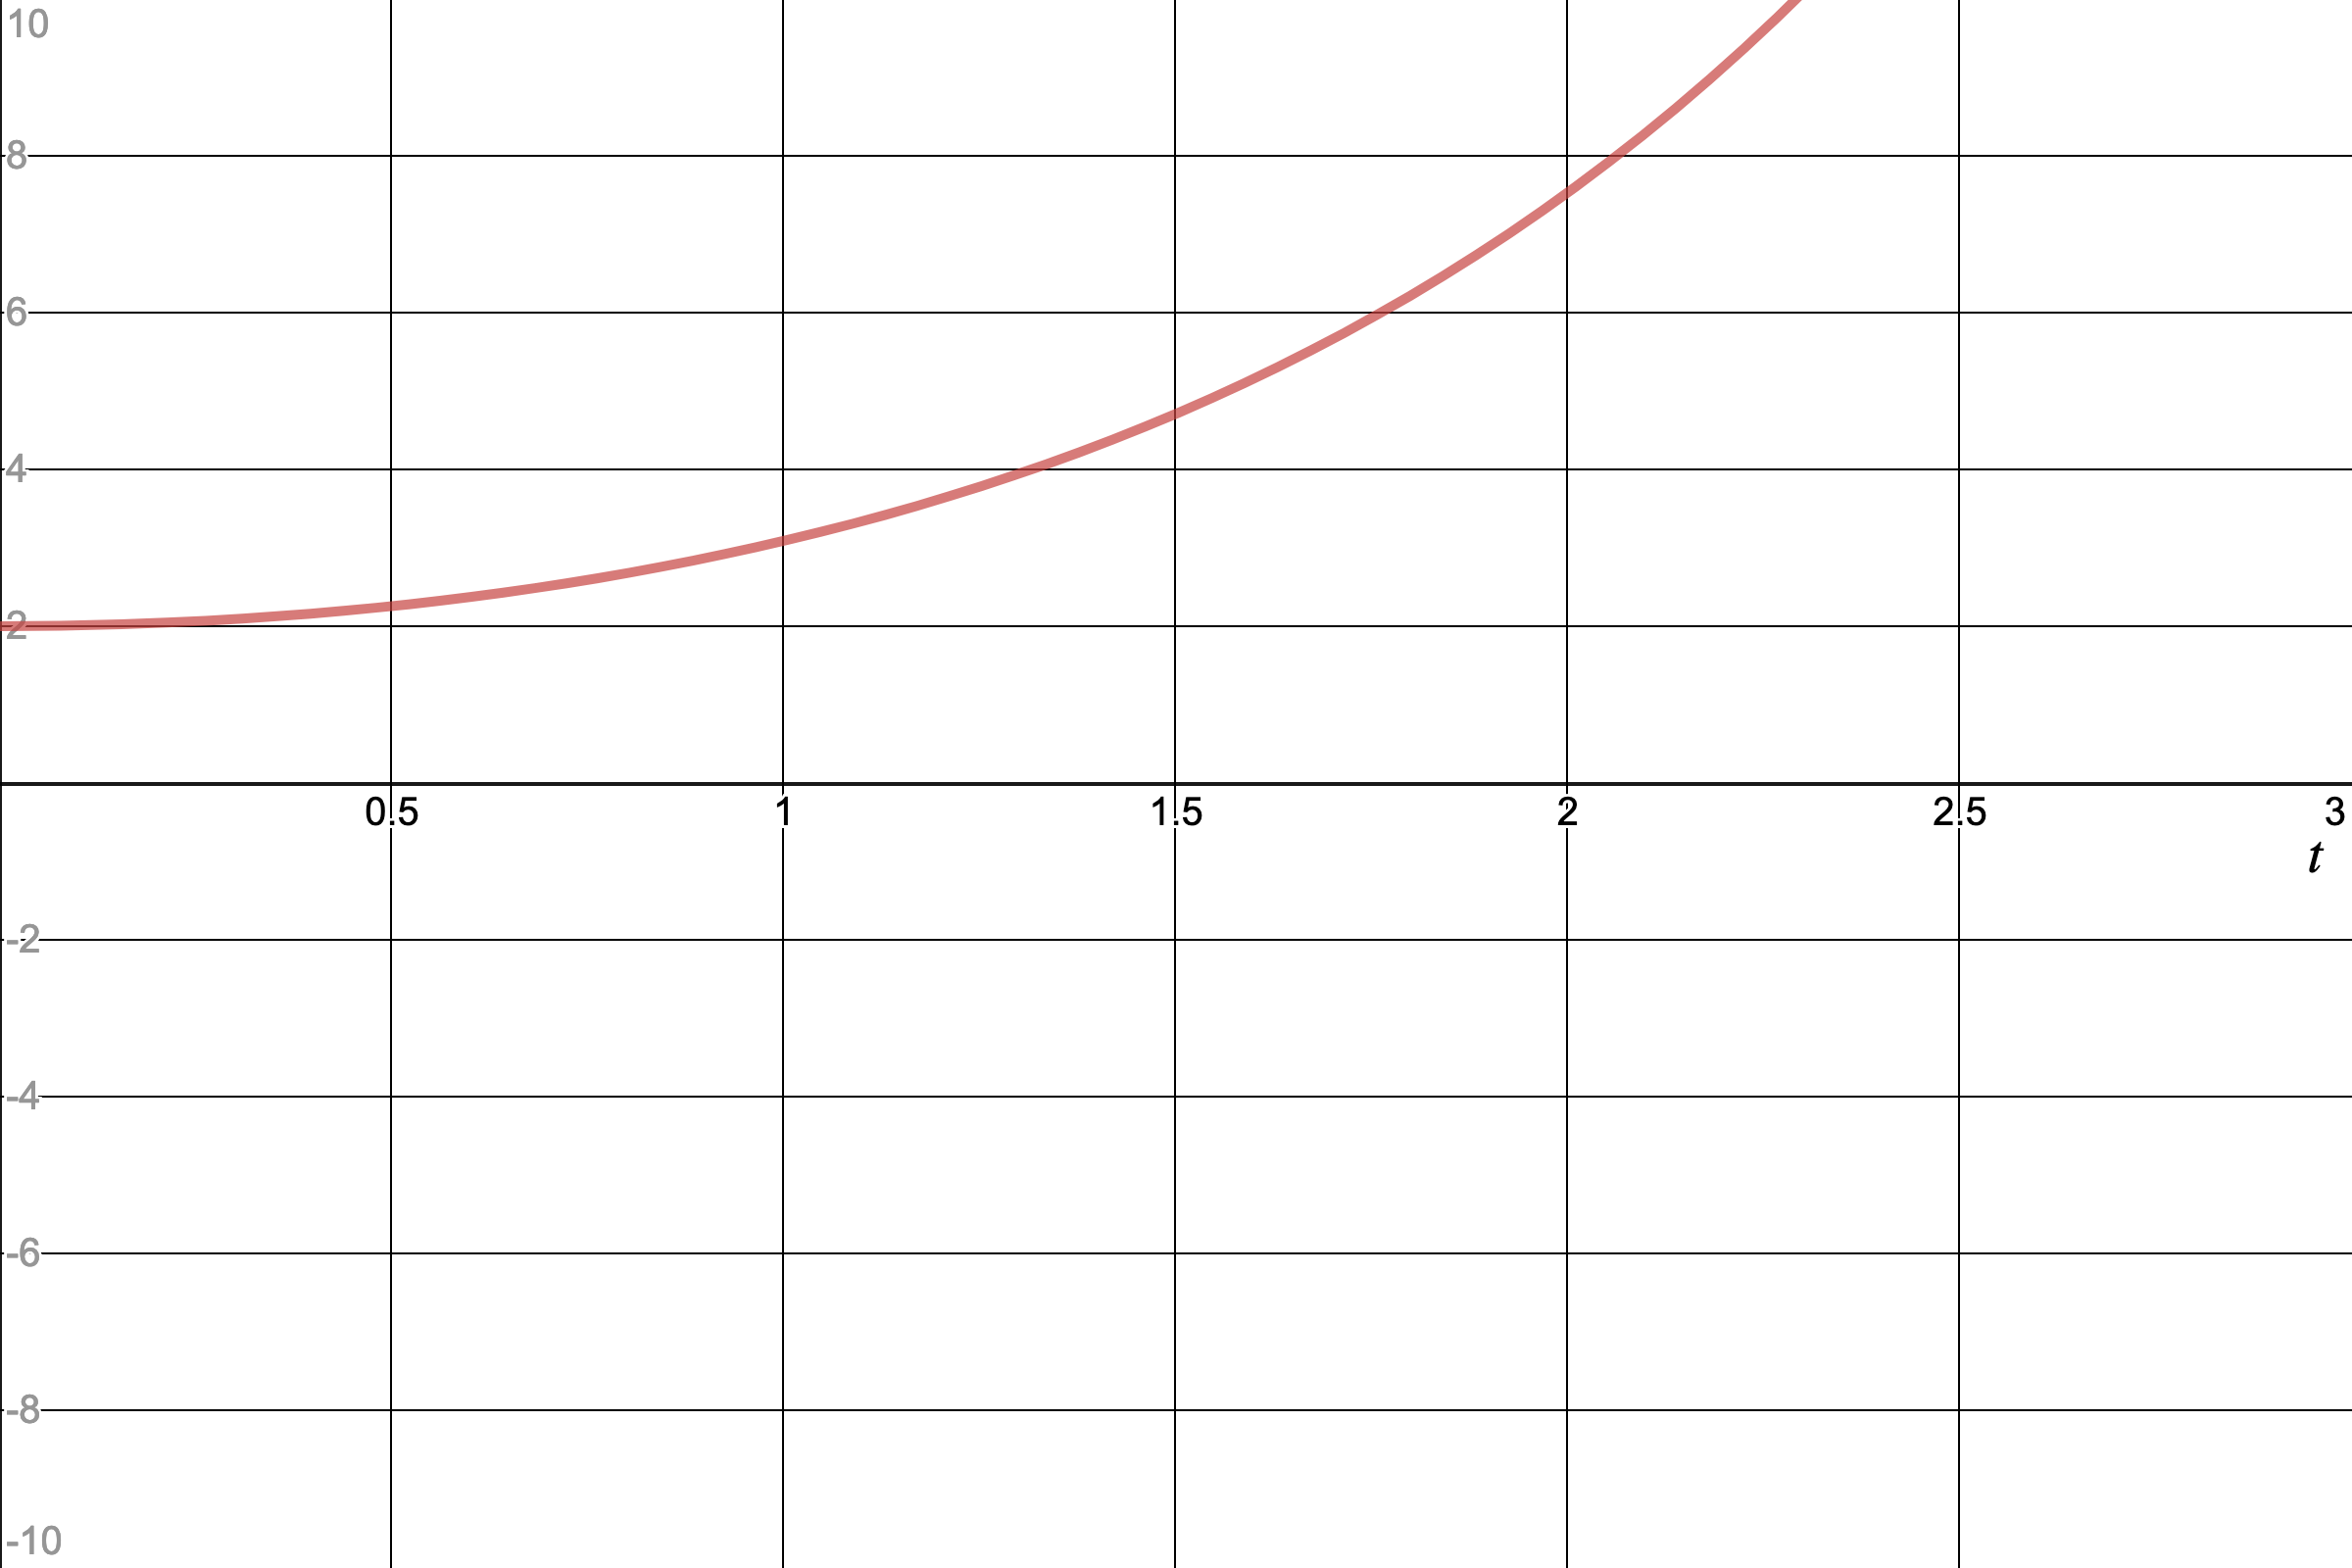
\includegraphics[width=.7\textwidth]{Figures_Part_2/l1=1_l2=-1.png}
                \end{figure}
                \item \textbf{Subcase 2:} If we have two identical real roots, $\lambda=\lambda_1=\lambda_2$ then the general solution is
                \[
                x(t)=C_1 e^{\lambda t}+C_2te^{\lambda t}.
                \]
                
                Here, we can take $\lambda=1$ and let $C_1=C_2=1$ and plot the solution:
                \begin{figure}[H]
                    \centering
                    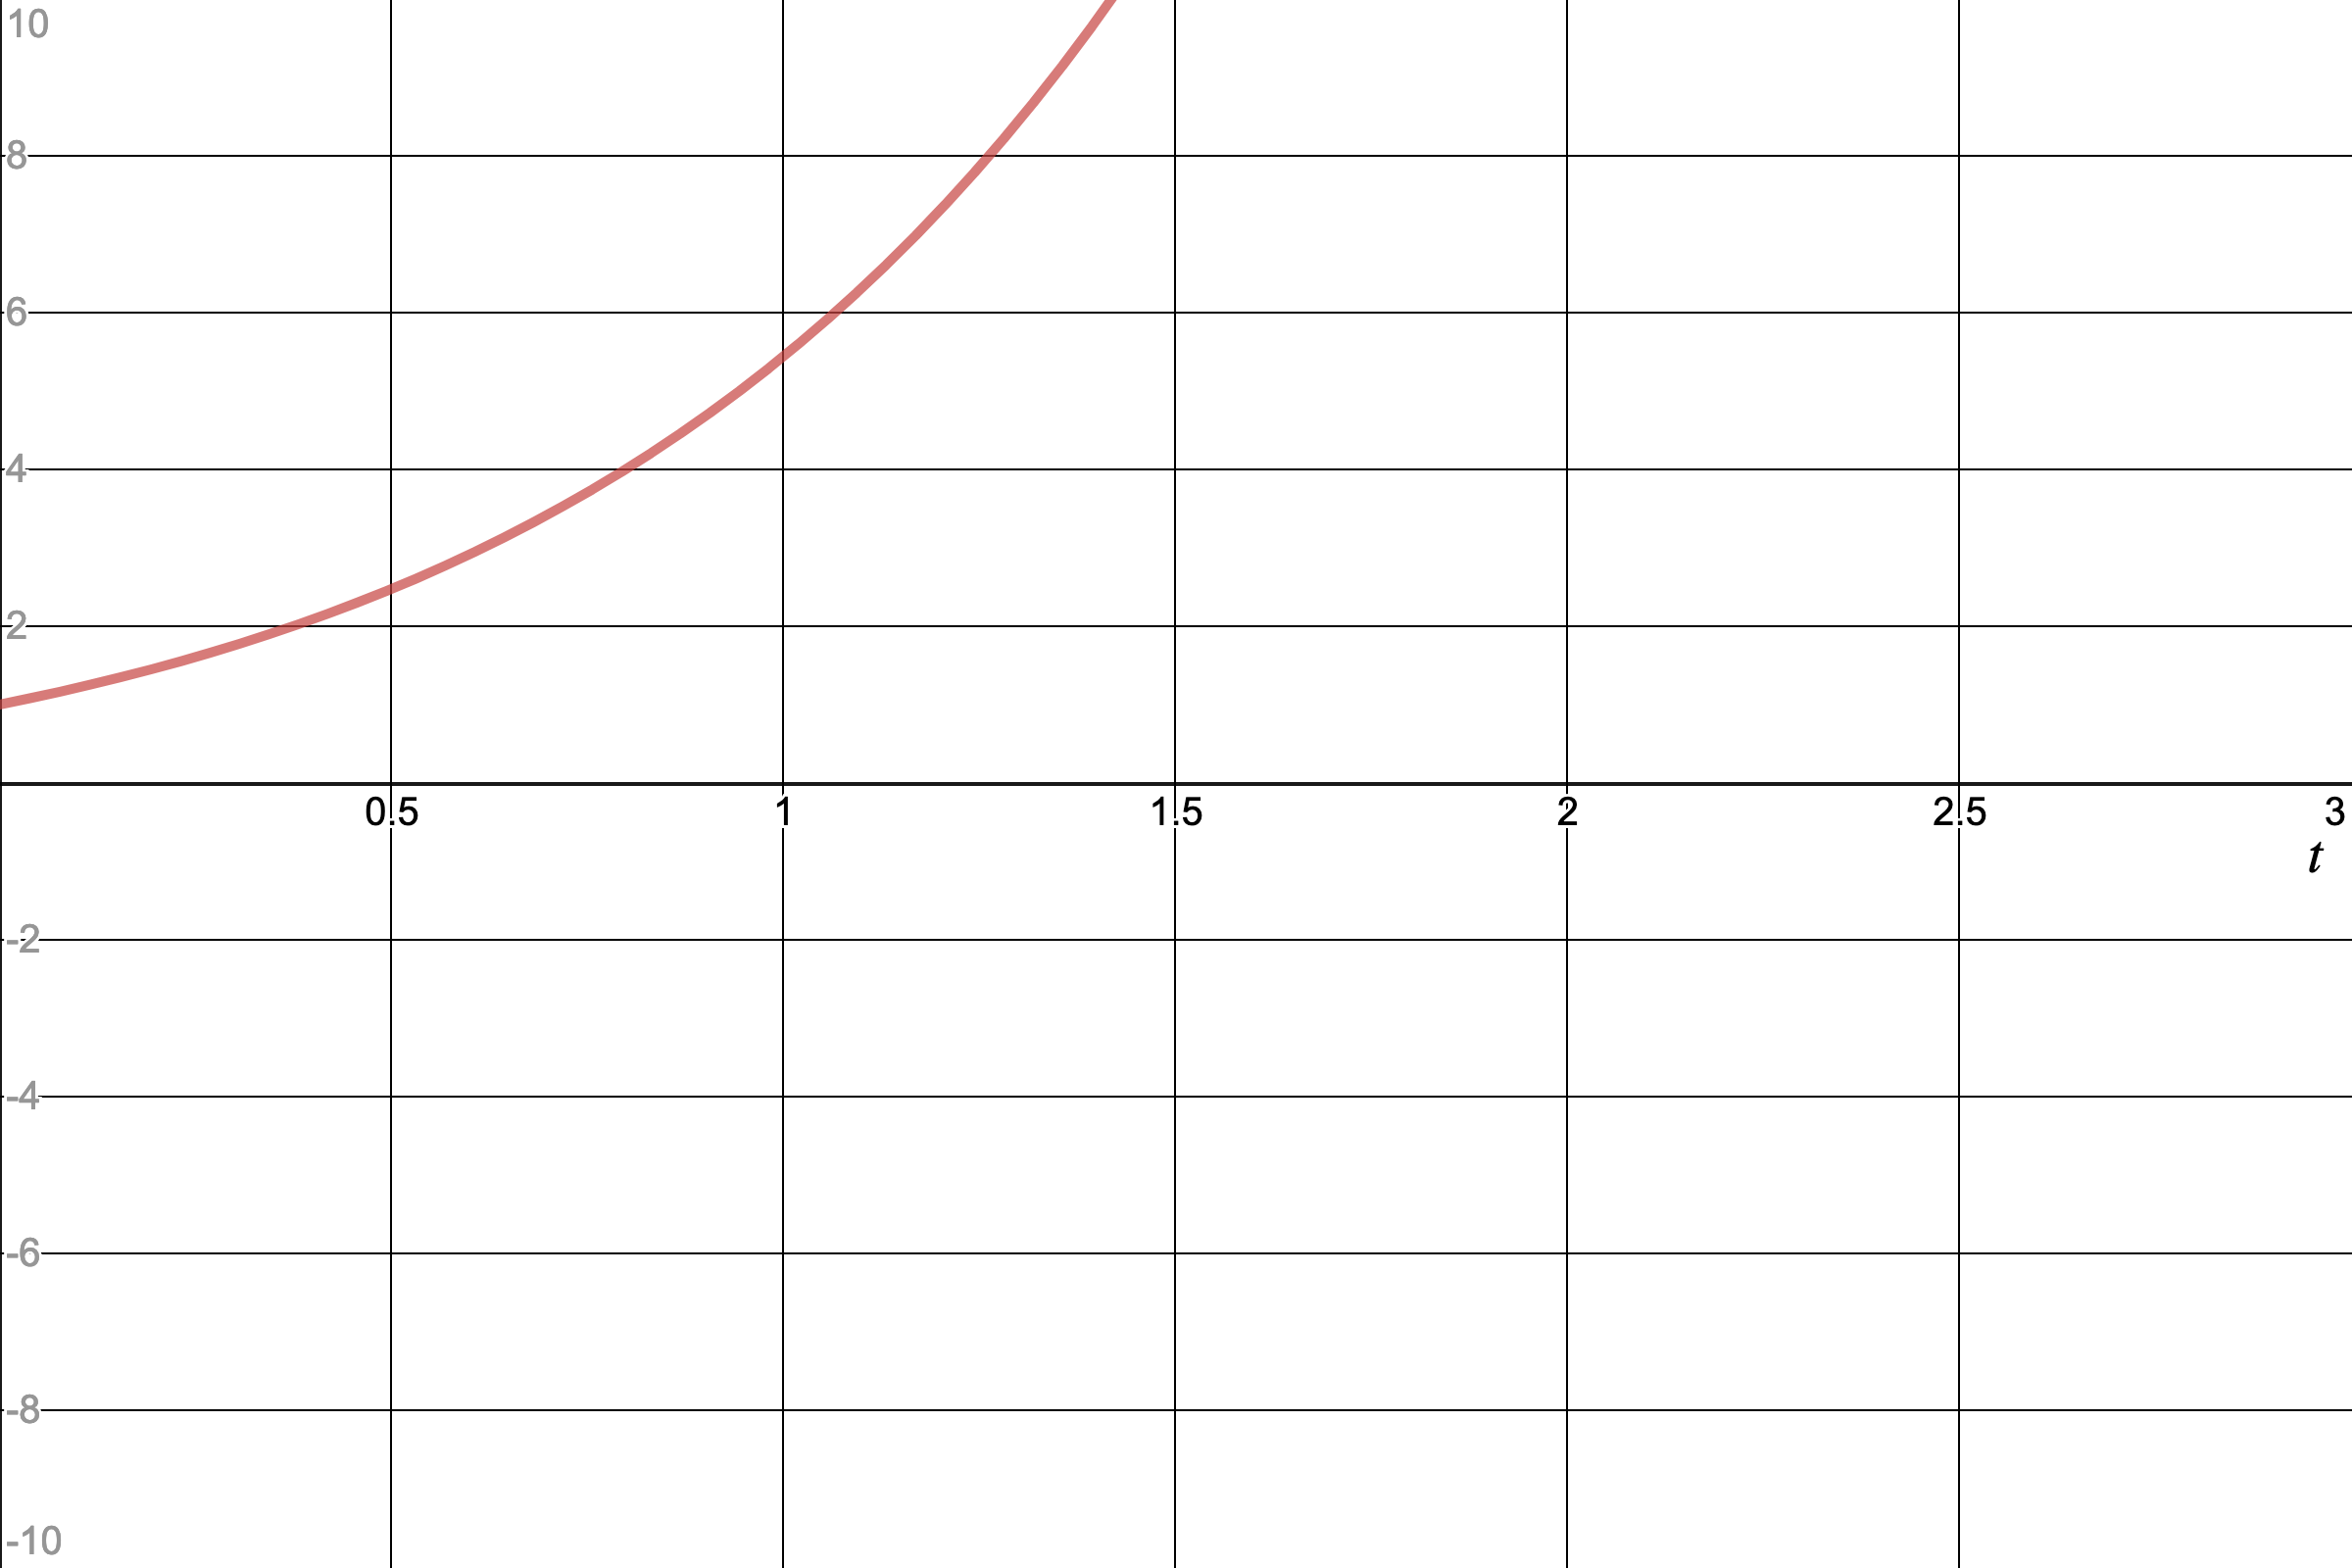
\includegraphics[width=.7\textwidth]{Figures_Part_2/l=1.png}
                \end{figure}
                We could also take $\lambda=-1$ with $C_1=C_2=1$ to see:
                \begin{figure}[H]
                    \centering
                    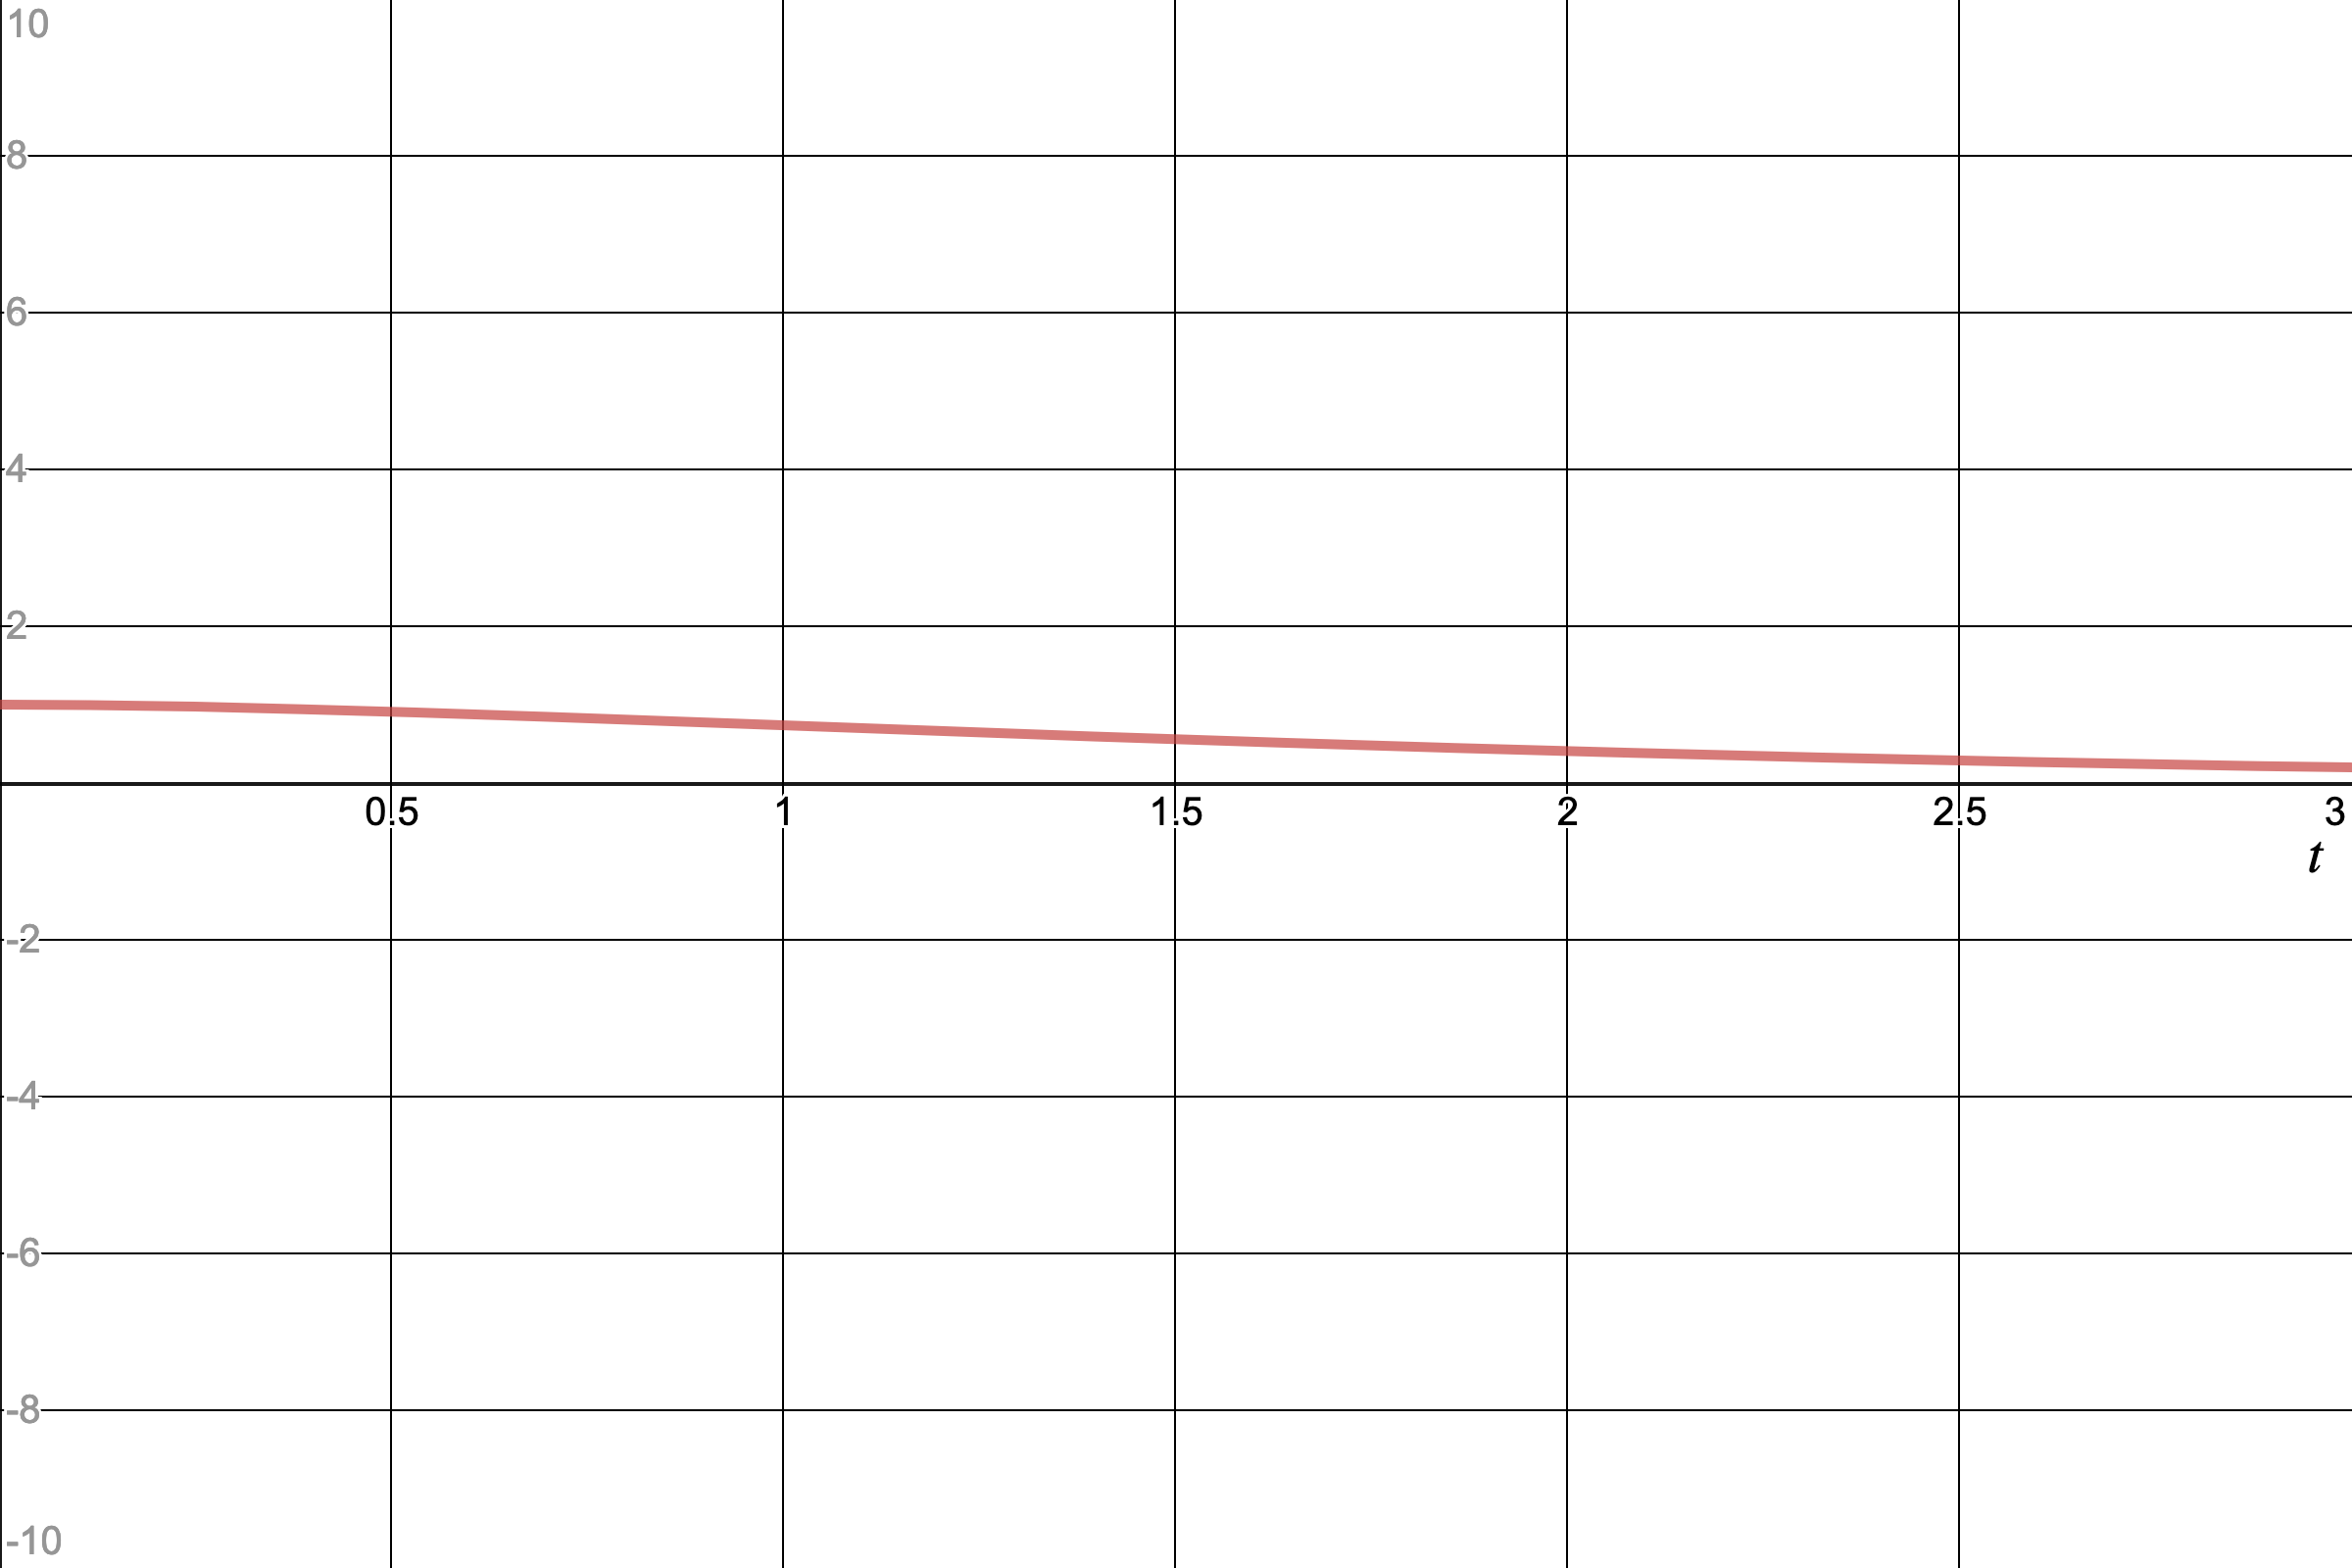
\includegraphics[width=.7\textwidth]{Figures_Part_2/l=-1.png}
                \end{figure}
            \end{itemize}
            \item \textbf{Case 2:} Consider the case where the roots to the characteristic polynomial are complex valued.  That happens when we have $b^2-4c$ since then we will have a square root of a negative number appear with the quadratic formula. In this case, if we have a root $\lambda$, then $\lambda^*$ is \underline{always} the other root (take a look at the quadratic formula, and see if you can see why this is the case).  Thus, we can put $\lambda=a+bi$ and then have another root $\lambda^*=a-bi$. This gives us the general solution
            \begin{align*}
                x(t)&= C_1 e^{\lambda t}+C_2 e^{\lambda^* t}\\
                &= C_1 e^{at}e^{ibt}+C_2e^{at}e^{-ibt}\\
                &= e^{at}\left( C_1 e^{ibt}+C_2 e^{-ibt}\right).
            \end{align*}
            Here, we must have that $C_1$ and $C_2$ are complex numbers.  We can also rewrite this general solution as
            \[
            x(t)= e^{at}(C_1 \cos(bt)+C_2\sin(bt)).
            \]
            
            Here we can take $a=1$ and $b=5$ with $C_1=C_2=1$ and plot the solution in the $xt$-plane to see:
            \begin{figure}[H]
                \centering
                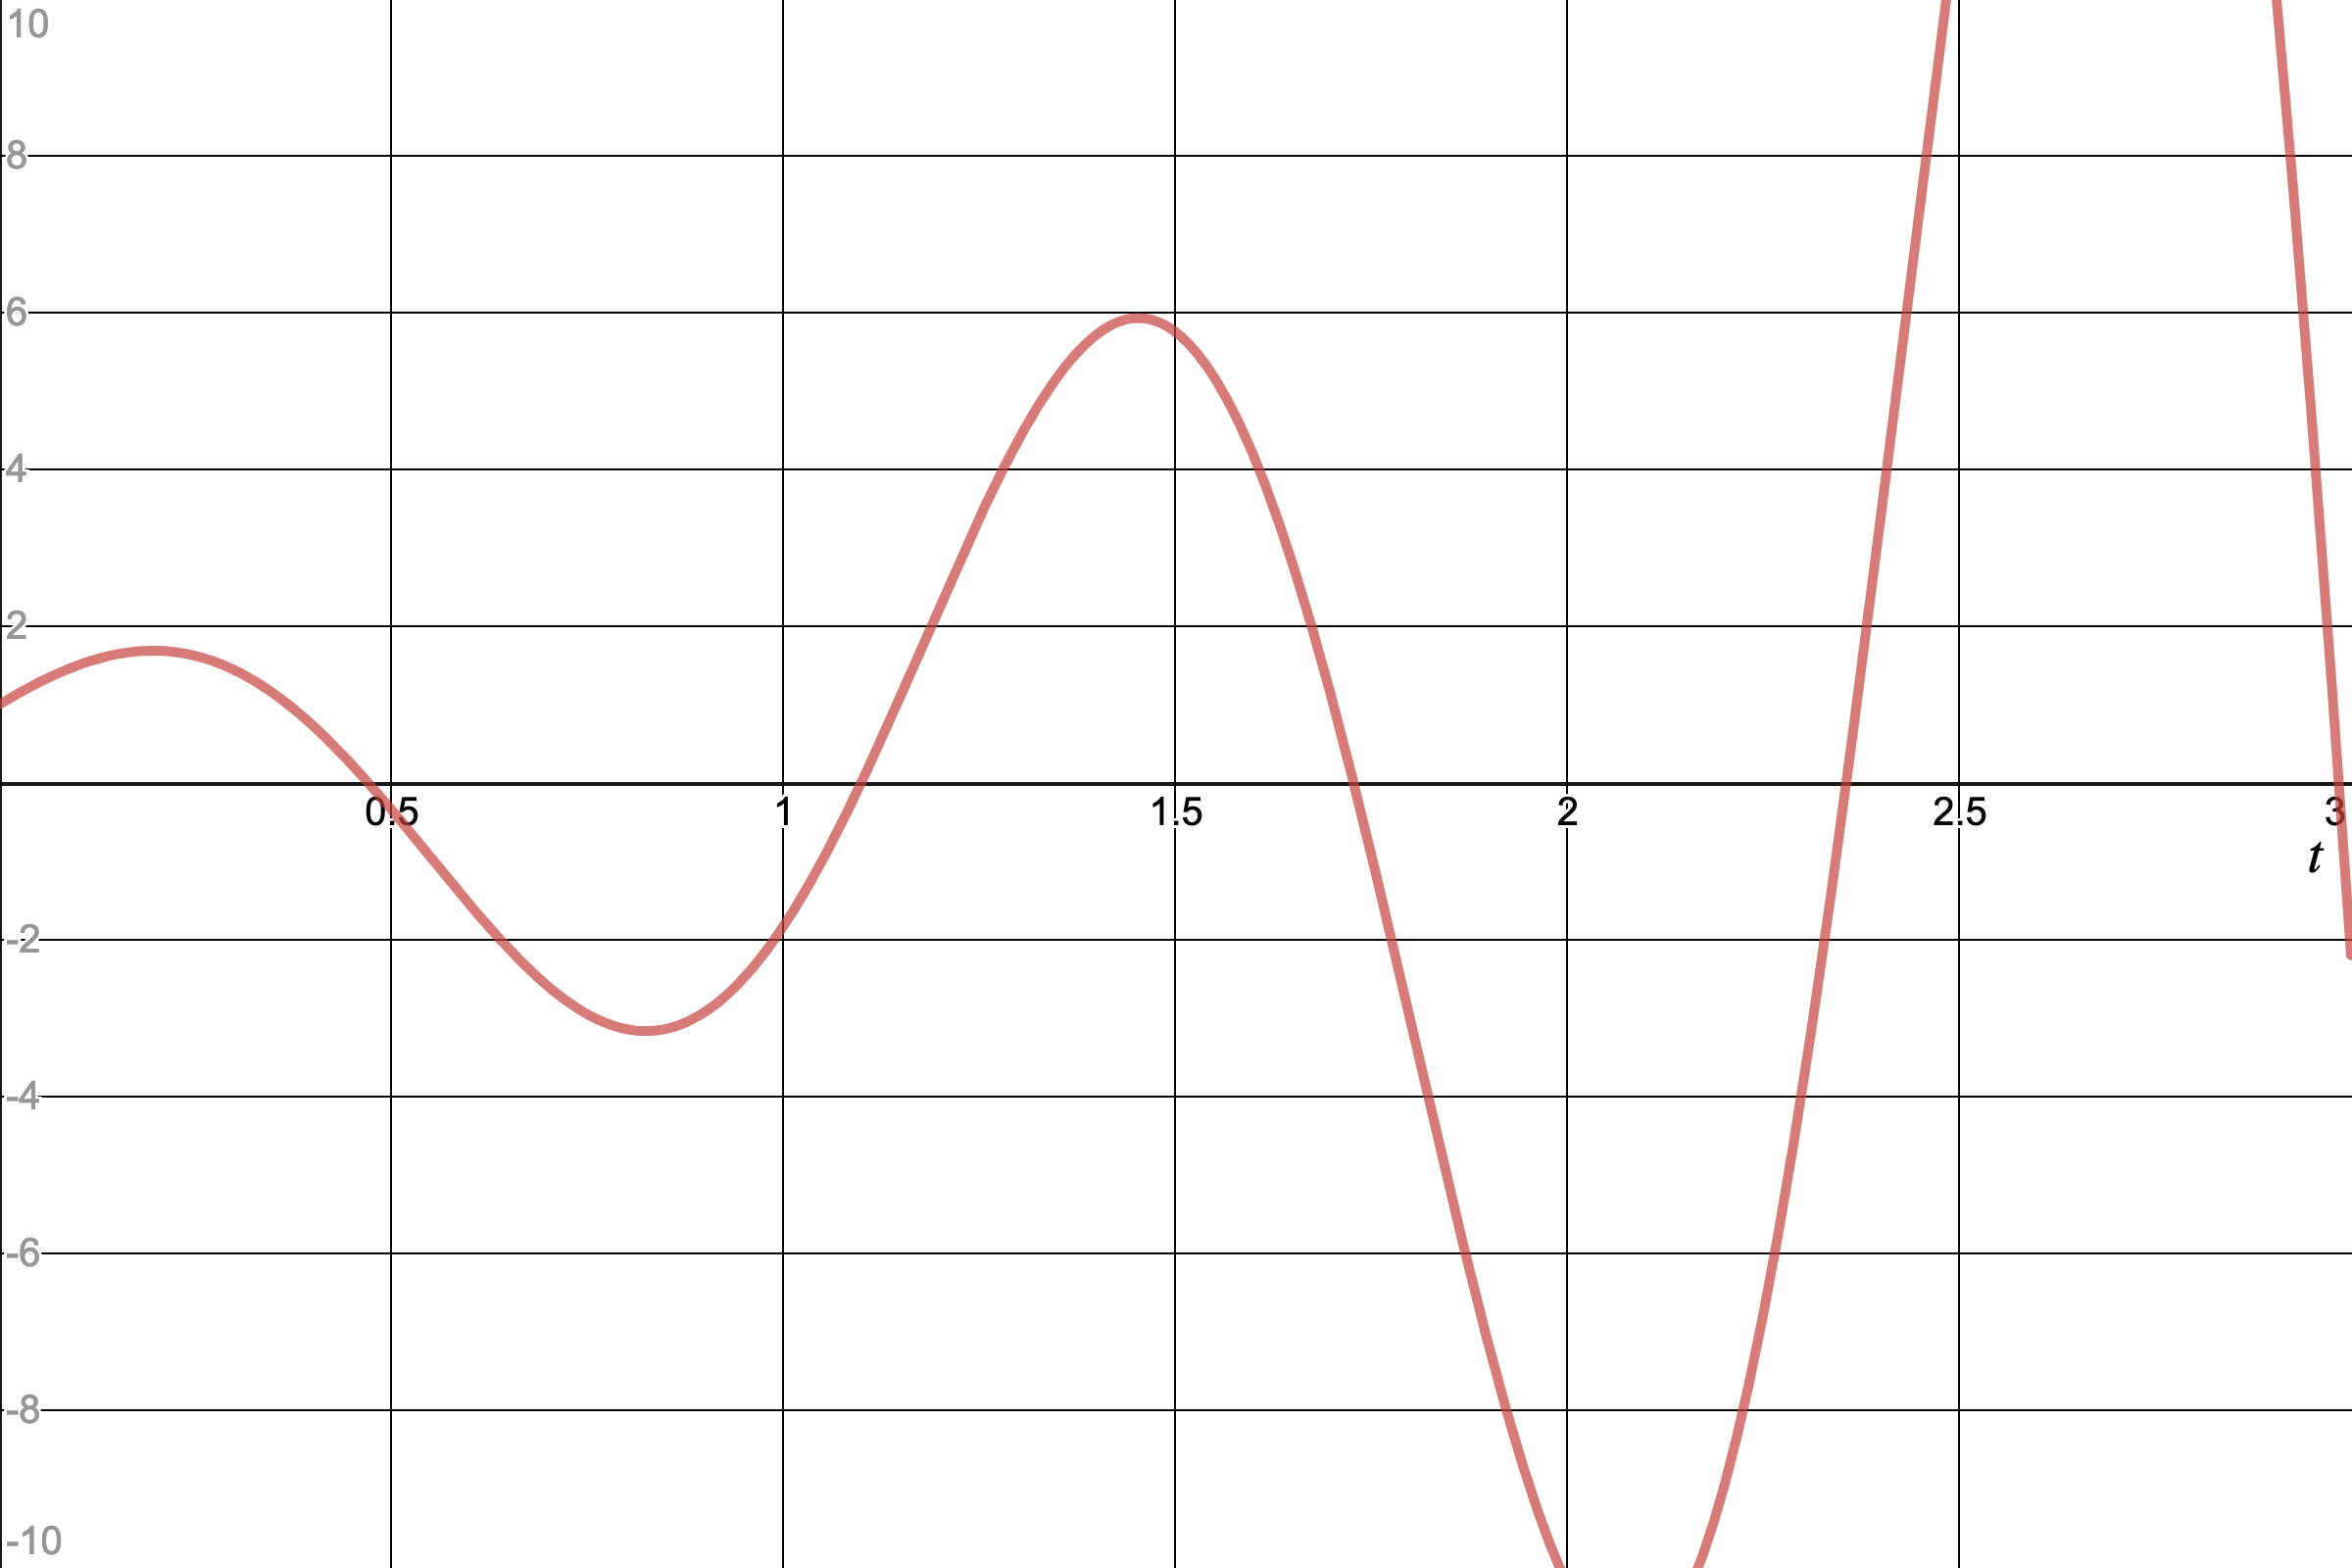
\includegraphics[width=.7\textwidth]{Figures_Part_2/a=1-b=5.png}
            \end{figure}
            We could also take the case with $a=0$, $b=5$, and $C_1=C_2=1$ and plot:
            \begin{figure}[H]
                \centering
                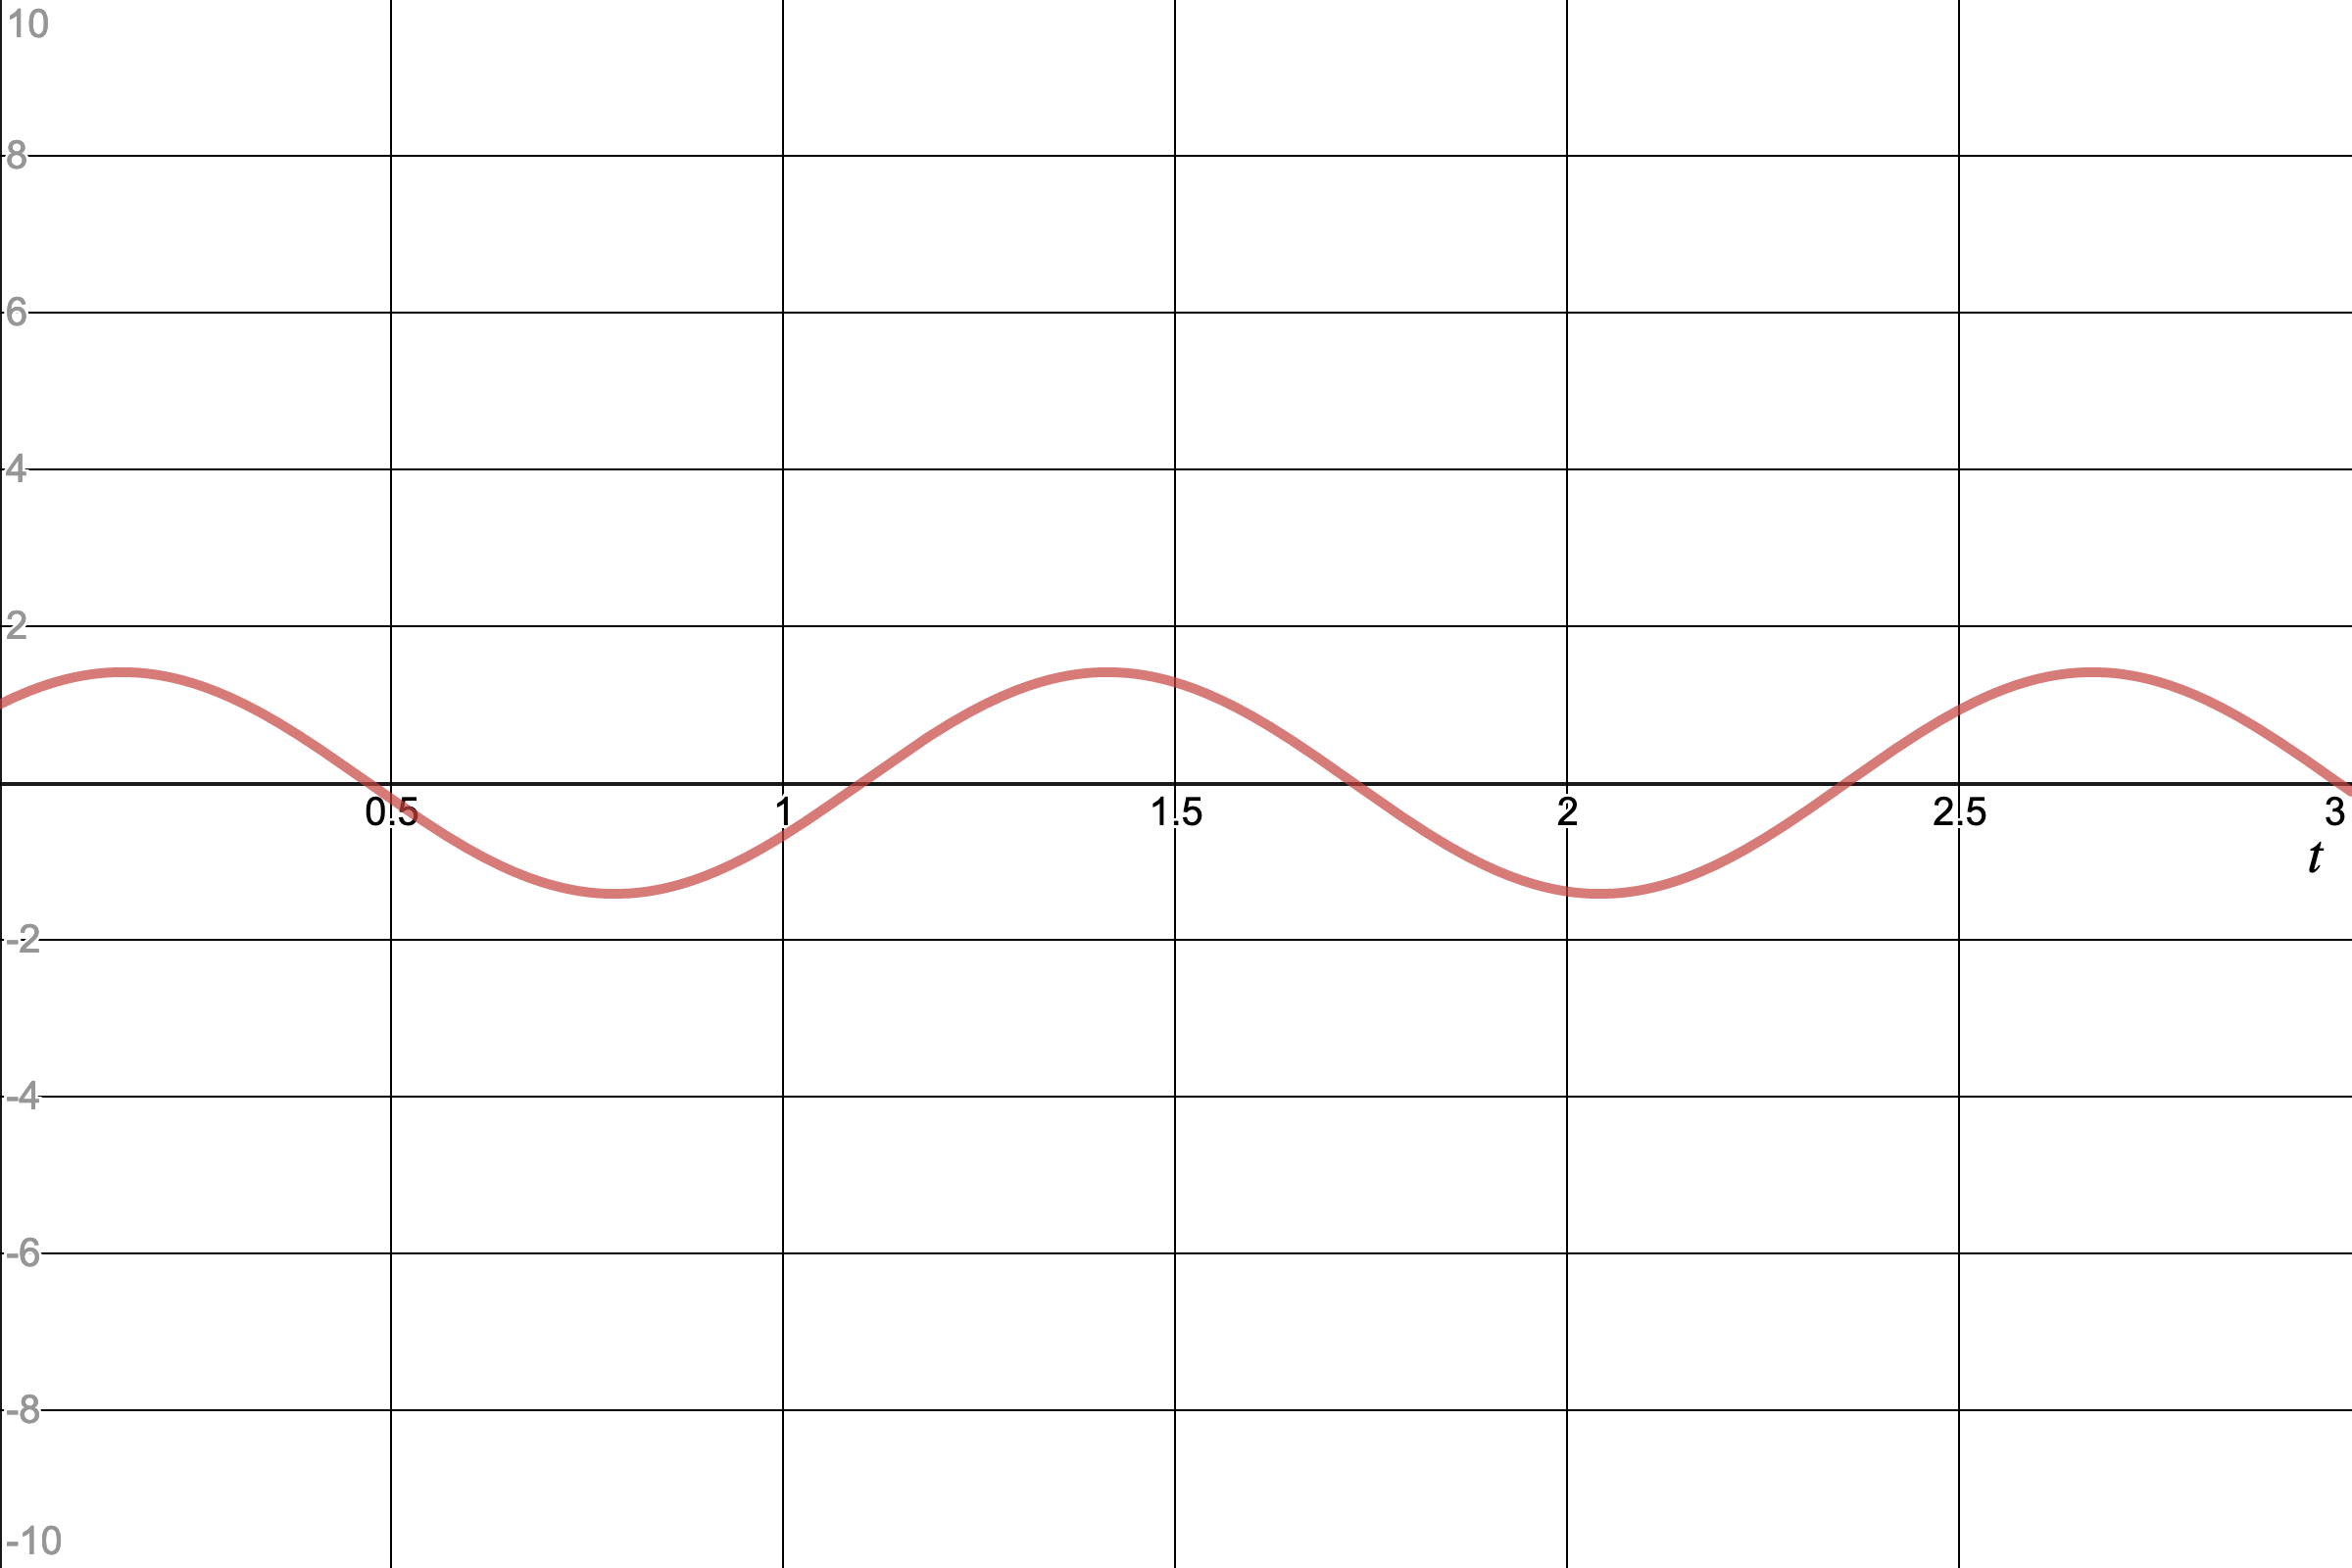
\includegraphics[width=.7\textwidth]{Figures_Part_2/a=0-b=5.png}
            \end{figure}
            Lastly, we could plot with $a=-1$, $b=5$ and $C_1=C_2=1$ to see:
                        \begin{figure}[H]
                \centering
                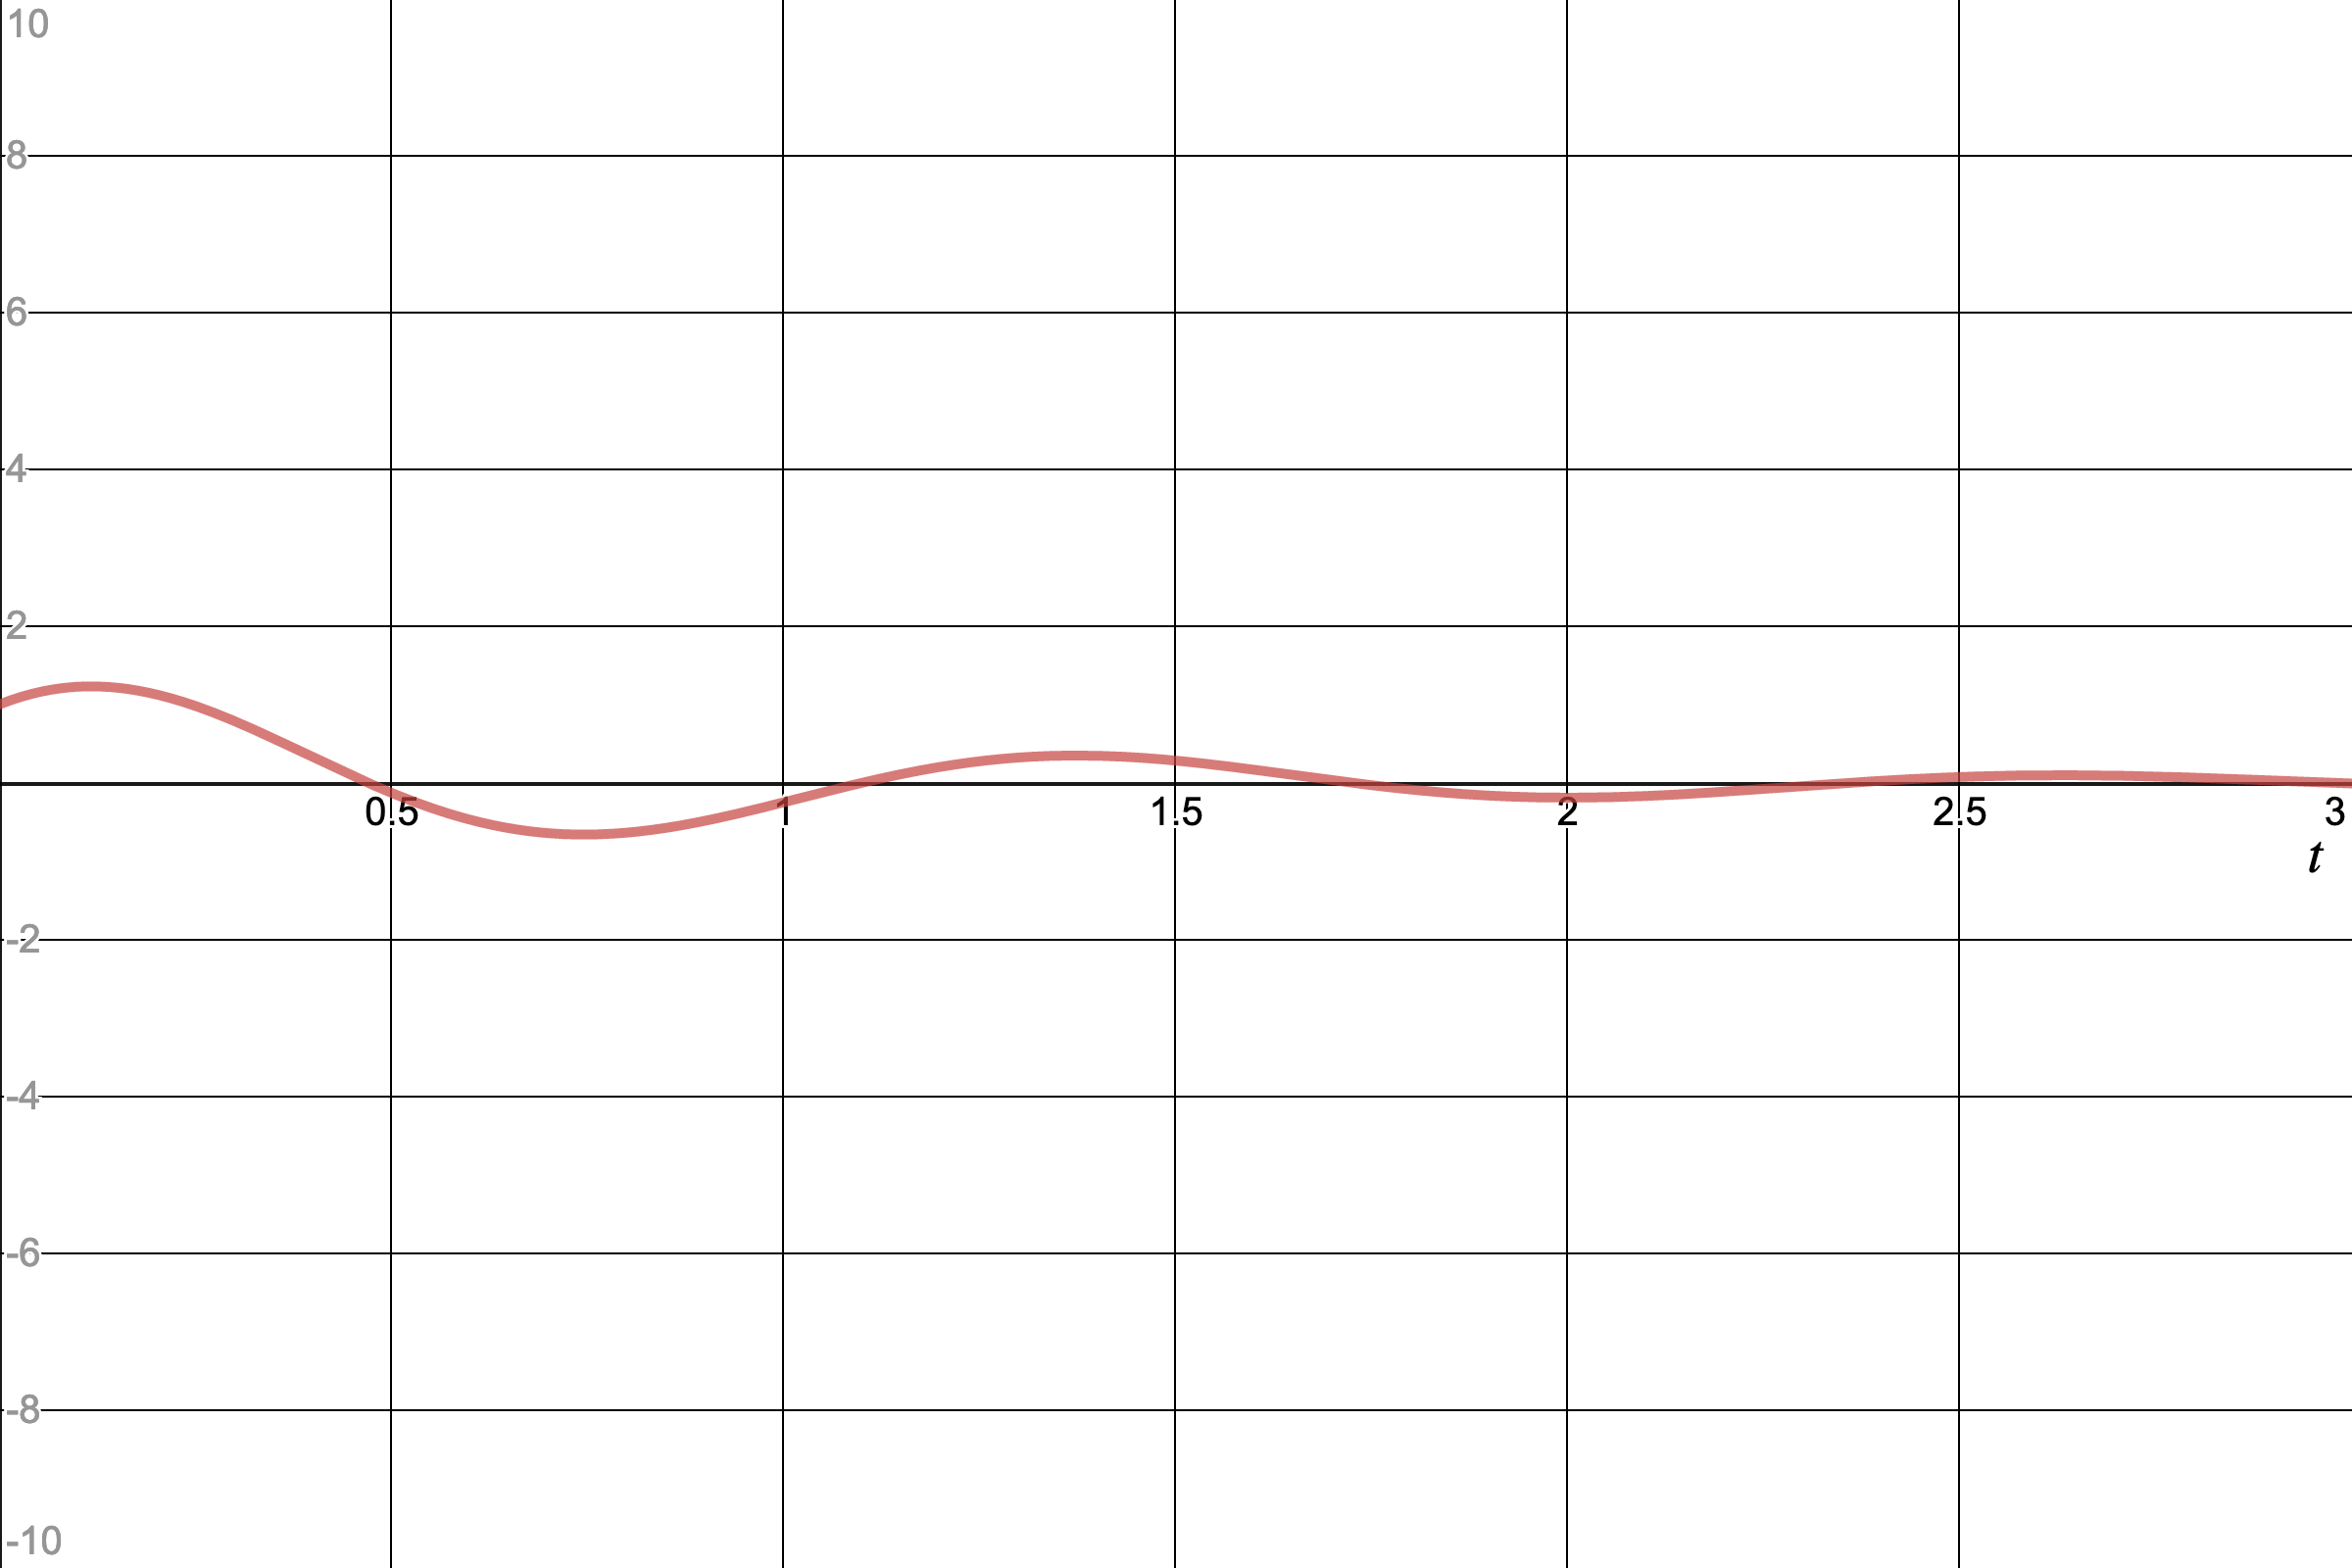
\includegraphics[width=.7\textwidth]{Figures_Part_2/a=-1-b=5.png}
            \end{figure}
        \end{itemize}
        
        \begin{exercise}
        Work out why if the roots to the characteristic polynomial are complex, that we always have the roots $\lambda$ and $\lambda^*$.
        \end{exercise}
        
        \begin{exercise}
        Show that the two general solutions
        \[
        x(t)=e^{at}(C_1 e^{ibt}+C_2e^{-ibt})
        \]
        and 
        \[
        x(t)=e^{at}(C_1 \cos(bt)+C_2\sin(bt))
        \]
        are equivalent using Euler's formula.
        \end{exercise}
        
        \subsection{Inhomogeneous Linear Equations}
        
        More often than not, we look at physical systems where there is some external force or potential that causes the system to change over time.  In the case of second order linear equations, this corresponds to the inhomogeneous equation
        \[
        x''+bx'+cx=F(t)
        \]
        where we think of $F(t)$ as an external force.  For specific forcing terms $F(t)$, we can solve this equation exactly using the \boldgreen{method of undetermined coefficients}\index{method of undetermined coefficients}.  The idea is that we can solve the homogeneous equation
        \[
        x_h''+bx_h'+cx_h=0
        \]
        to find a solution $x_h(t)$.  We refer to this as the \boldgreen{homogeneous solution}\index{homogeneous solution}. It does not, however, solve the equation on its own. We then need another function which we call the \boldgreen{particular integral}\index{particular integral} and denote by $x_p(t)$. This function is given by an ansatz based on what the forcing term is.  In this case, $x_p(t)$ solves the inhomogeneous equation
        \[
        x_p''+bx_p'+cx_p=F(t)
        \]
        but is needs to be accompanied by a homogeneous solution. The solution to an inhomogeneous equation as above will then be
        \[
        x=x_h+x_p.
        \]
        How do we know that this is a solution? We can check by taking
        \begin{align*}
            x''+bx'+cx&=(x_h+x_p)''+b(x_h+x_p)'+c(x_h+x_p)\\
            &= \underbrace{(x_h''+bx_h'+cx_h)}_{=0}+\underbrace{(x_p''+bx_p'+cx_p)}_{=F(t)}\\
            &=F(t).
        \end{align*}
        So the sum of a particular integral and a homogeneous solution is also a solution to the inhomogeneous equation! Now, let's see an example.
        
        \begin{ex}{Inhomogeneous Linear Equation with Constant Force}{inhom_linear}
        If we assume our equation has a quadratic forcing term $F(t)=2t^2$, then we have the equation
        \[
        x''+3x'+2x=2t^2.
        \]
        First, we find the solution to the homogeneous equation
        \[
        x_h''+3x_h'+2x_h=0
        \]
        which has the characteristic polynomial
        \[
        \lambda^2+3\lambda+2=0.
        \]
        The roots are then $\lambda_1=-1$ and $\lambda_2=-2.$ So we have that
        \[
        x_h(t)=C_1e^{-t}+C_2e^{-2t}.
        \]
        Next, we take an ansatz of $x_p(t)=a_0+a_1t+a_2t^2$ and call the $a_i$ coefficients the \boldgreen{undetermined coefficients}.  Then we have
        \[
        x_p'=a_1+2a_2t \qquad \textrm{and} \qquad x_p''=2a_2.
        \]
        We can plug these into our inhomogeneous equation
        \begin{align*}
        x''+3x'+2x&= 2a_2+3(a_1+2a_2t)+2(a_0+a_1t+a_2t^2)
        \end{align*}
        which we know should also be equal to the forcing term $F(t)$.  This gives us the equation
        \[
        2a_2+3(a_1+2a_2t)+2(a_0+a_1t+a_2t^2)=2t^2.
        \]
        We rearrange the terms as follows
        \[
        (2a_0+3a_1+2a_2)+(2a_1+6a_2)t+(2a_2)t^2=0+0t+2t^2
        \]
        which gives us the system of equations
        \begin{align*}
            2a_0+3a_1+2a_2&=0\\
            2a_1+6a_2&=0\\
            2a_2&=2.
        \end{align*}
        We can solve these to find $a_2=1$, $a_1=-3$ and $a_0=\frac{7}{2}$. So the particular integral is $x_p(t)=t^2-3t+\frac{7}{2}$.  Thus we have a solution
        \[
        x=x_h+x_p=C_1e^{-t}+C_2e^{-2t}+t^2-3t+\frac{7}{2}.
        \]
        If we were given initial data, we could solve for $C_1$ and $C_2$.
        \end{ex}
        
        
        \noindent Here's a table of the forms of $F(t)$ which will be solvable. You can use this to find an ansatz for the particular integral.  Once you know the ansatz it comes down to solving for the coefficients as we did in the previous example.
        \begin{table}[H]
        \centering
        \renewcommand{\arraystretch}{1.75}
            \begin{tabular}{c|c}
                Forcing Term $F(t)$&  Particular Integral $x_p$\\
                \hline
                $ke^{at}$ & $Ce^{at}$\\
                \hline
                $kt^n$ ~ $(n=0,1,2,\dots)$ & $\sum_{j=0}^n a_j t^j$\\
                \hline
                $k\cos(at)$ ~\textrm{or}~ $k\sin(at)$ & $K\cos(at)+M\sin(at)$\\
                \hline
                $ke^{at}\cos(bt)$ ~\textrm{or}~ $ke^{at}\sin(bt)$ & $e^{at}(K\cos(bt)+M\sin(bt))$\\
                \hline
                $\displaystyle{\left(\sum_{j=0}^n k_jt^j\right) \cos(bt)}$ ~\textrm{or}~ $\displaystyle{\left(\sum_{j=0}^n k_jt^j\right) \sin(bt)}$ & $\displaystyle{\sum_{j=0}^n\left( Q_jt^j \cos(bt) + R_jt^j \sin(bt)\right)}$\\
                \hline
                $\displaystyle{\left(\sum_{j=0}^n k_jt^j\right) e^{at}\cos(bt)}$ ~\textrm{or}~ $\displaystyle{\left(\sum_{j=0}^n k_jt^j\right) e^{at}\sin(bt)}$ & $\displaystyle{e^{at}\left(\sum_{j=0}^n \left( Q_jt^j \cos(bt) + R_jt^j \sin(bt)\right)\right)}$
            \end{tabular}
    \end{table}


        
        \newpage
        \section{Problems}
        \textcolor{blue}{to come}
        

        


\chapter{Boundary Value Problems}
        
There is another kind of problem we care to work with.  All the problems we have considered have been initial value problems. However, there is a completely different type of problem we can solve.  This will be called a \boldgreen{boundary value problem}.  Let us make a comparison.

\subsubsection{Second Order Initial Value Problem}
\begin{itemize}
    \item Given a very general second order equation $x''=f(t,x,x')$ and initial data $x(0)=x_0$ and $x'(0)=v_0$.  
    \item Both conditions are given at the initial time $t=0$. We have one condition $x(0)$ for position and the other $x'(0)$ for velocity 
    \item Think of the solution $x(t)$ of tracking a particle over time. 
\end{itemize}

\subsubsection{Second Order Boundary Value Problem}
\begin{itemize}
    \item Given a very general second order equation $u''=f(x,u,u')$ and a \emph{region} $\Omega=[a,b]$ with \emph{boundary values} $u(a)=u_a$ and $u(b)=u_b$.
    \item Conditions are given at the endpoints of a region $\Omega=[a,b]$.  There will be one condition for every endpoint $a$, and $b$. The values will be given as $u(a)=u_a$ and $u(b)=u_b$. (\emph{Note: we may also prescribe slightly different conditions later on. These are referred to as Dirichlet boundary conditions.})
    \item Think of solution $u(x)$ as modeling a measurable quantity of an object (i.e., temperature, height, stress, or strain).
\end{itemize}

Boundary value problems are very important in the physical world.  For example, an engineer may wish to understand how a rod is deformed under the force of gravity as well as whatever machinery is pulling and pushing on it.  The engineer would hope to understand this deformation so that they can build sturdy structures.  In the field of chemistry, we see boundary value problems arise in thermal or quantum transport, in chemical reactions, in waves or lattice vibrations, and more. 

Not all boundary value problems are second order.  However, we'll concentrate first on problems that are second order as they are more pertinant for us.  The equations we'll start with will be Laplace's (or Poisson's) equation and then we'll move onto Schr\"odinger's equation.

\section{Laplace's and Poisson's Equations}

Let us set up the problem at hand.  We'll define our first boundary value problem as such.
\begin{df}{Boundary Value Problem}{boundary_val}
A \boldgreen{boundary value problem} is a differential equation (of possibly multiple variables) defined on a region in space $\Omega$ with prescribed \boldgreen{boundary data} (i.e., functions defined on the boundary of the region $\Omega$).  

For now, all regions will be $\Omega=[a,b]$, the \boldgreen{boundary} is the set $\{a,b\}$, and the differential equations will be second order.
\end{df}

\begin{remark}
Here, I will use the notation
\[
\frac{d}{dx}u=u'
\]
since we often like to think of $\frac{d}{dx}$ as an \emph{operator}.  We will get more into this later. Right now, it's just equivalent notation.
\end{remark}

\begin{ex}{Laplace's Equation: Dirichlet Boundary Data}{laplace}
\emph{Imagine a rod of length $L$ attached at endpoints $x=0$ and $x=L$.  The height of the endpoints of the rod are $u(0)=1$ and $u(L)=0$ respectively.  The rod is experiencing no external forces.  What is the shape of the rod?}\\

This problem statement leads us to consider the following boundary value problem
\[
\frac{d^2}{dx^2}u(x)=0
\]
on the region $\Omega = [0,L]$ with boundary data $u(0)=1$ and $u(L)=0$. Here, we are providing the function value that $u(x)$ must satisfy on the boundary.  Everywhere inside $\Omega$ (i.e., $(0,L)$), $u(x)$ must satisfy the differential equation as well. 

We know how to solve this equation as we can just integrate twice.  We find that the general solution is
\[
u(x)=C_1 x + C_2.
\]
We can solve for the constants $C_1$ and $C_2$ by using our boundary data. We require
\begin{align*}
    1&=u(0)=C_1(0)+C_2=C_2\\
    0&=u(L)=C_1(L)+C_2.
\end{align*}
The first equation gives us $C_2=1$ which we can plug into the second to get
\[
0=C_1(L)+C_2
\]
which means that $C_1=-\frac{1}{L}$.  Thus our particular solution to this boundary value problem is
\[
\boxed{u(x)=-\frac{1}{L}x+1.}
\]
\end{ex}

\begin{exercise}
Plot the above solution and verify it satisfies the ODE and the boundary values.  What can we say about the shape of the rod? Is is what we would expect?
\end{exercise}

So, the set up to these problems is a bit different, but solving them is fundamentally the same idea. Let's see some other examples of different equations.

\begin{df}{Laplace and Poisson Equations}{laplace_poisson}
On a region $\Omega=[a,b]$ we prescribe boundary data $u(a)=u_a$ and $u(b)=u_b$.  On this region, \boldgreen{Laplace's equation} is
\[
\frac{d^2}{dx^2}u(x)=0
\]
and \boldgreen{Poisson's equation} is 
\[
-\frac{d^2}{dx^2}(x)=F(x)
\]
for some given function $F(x)$. If this $F(x)$ is of the form $ku(x)$ for some constant $k$, then we have the equation for \boldgreen{eigenfunctions of the Laplacian}
\[
\frac{d^2}{dx^2}(x)=ku(x).
\]
We'll see that this equation shows up in quantum mechanics.
\end{df}

If we read the two examples and the definition of the Laplace and Poisson equations, we can get an intuition on what they're describing.  In a sense, both equations can describe the curvature of a 1-dimensional object.  Why is that? The second derivative gives us information about the curvature of a function at each point! For the Laplace equation, the curvature is said to be zero everywhere, hence when we integrated and found a solution, we found that we got a linear equation with some unknown coefficients that we could find with boundary data.  For the Poisson equation, however, there is some external force function $F(x)$ that deforms the rod.  So, the curvature should not be zero everywhere, which gives us a different set of solutions.  One may also notice that the solution to the Laplace equation appeared within the solution to the Poisson equation (go back and reread both to see this).  This is very much like solving homogeneous versus inhomogeneous second order linear ODEs with constant coefficients.

\begin{ex}{Poisson's Equation: Dirichlet Boundary Data}{poisson_neumann}
\emph{Consider a cable of length $1$ attached at endpoints $x=0$ and $x=1$.  Now, the attachment points of the cable is prescribed by specifying $u(0)=0$ and $u(1)=0$. The cable is also being pushed down by a constant force (like gravity). That is, $F(x)=-1$ constantly pulls the cable down.  We expect this cable to sag under this force much like power lines due under the force of gravity.}\\

This gives us the boundary value problem
\[
-\frac{d^2}{dx^2}(x)=-1
\]
on the region $\Omega = [0,1]$ with boundary data $u(0)=0$ and $u(1)=0$. We can integrate this equation twice to get
\[
u(x)= \frac{1}{2}x^2+bx+c.
\]
Now, we can use our boundary data to try and solve this problem. We require
\begin{align*}
    0=u(0)&=c,
\end{align*}
and hence $c=0$.  Thus, at this point we have $u(x)=\frac{1}{2}x^2+bx$.  The second equation from the second boundary value is then
\[
u(1)=\frac{1}{2}+b,
\]
and so $b=-\frac{1}{2}$. Hence our particular solution to the boundary value problem is
\[
\boxed{u(x)=\frac{1}{2}x^2-\frac{1}{2}x.}
\]
We can plot this solution and see if this makes physical sense.
\begin{figure}[H]
    \centering 
    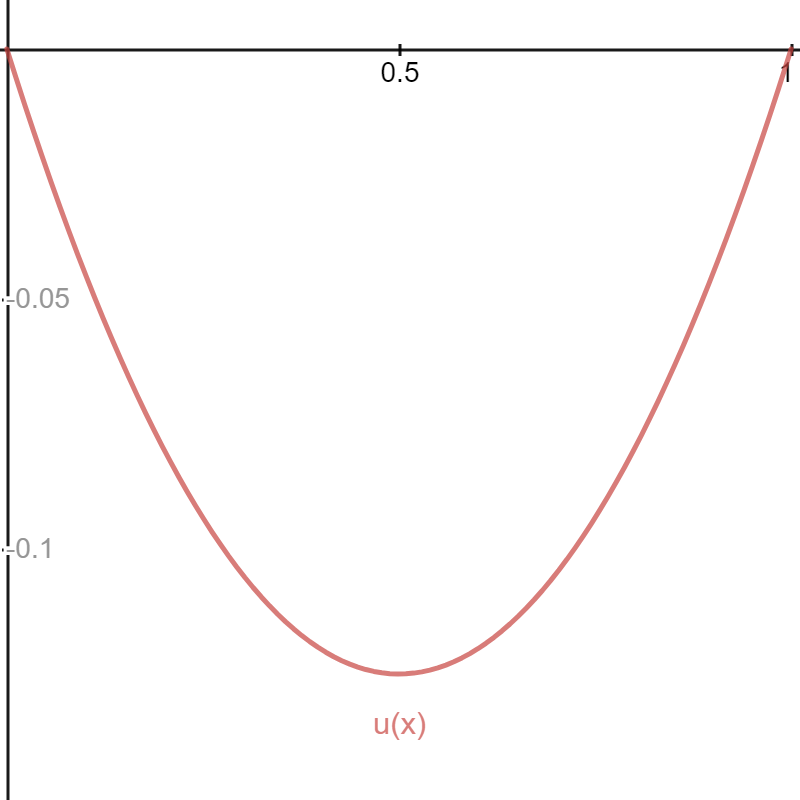
\includegraphics[width=.6\textwidth]{Figures_Part_1/poisson_equation_gravity.png}
    \caption{The profile of a cable under a constant force directed downward.}
\end{figure}

It seems like the curvature of this cable is close to what we would expect.  How much deformation there is would depend on the strength of the force $F(x)$ as well as the elastic properties of the cable.  These would all factor in to the equation if we considered it in greater detail.
\end{ex}

\section{A Particle in a 1-Dimensional Box}

Now, let's enter into some quantum mechanics.  In essence, quantum mechanics is governed by the \emph{Schr\"odinger equation}.  Think of this equation as a quantum version of Newton's laws.  The equation describes the state of a particle which we denote by $\psi(x)$.  If we put $\psi(x)$, we are thinking of this particle as not evolving in time, but having this function describing its position nonetheless.  We call a function $\psi$ that solves Schr\"odinger's equation a \emph{wavefunction}.  The wavefunction is not quite physically meaningful in its own right.  However, it gives rise to a probability interpretation of the particle. We'll see that shortly.

\begin{df}{Time Independent Schr\"odinger Equation}{time_ind_schro}
The \boldgreen{one dimensional time independent Schr\"odinger equation} with \boldgreen{potential} $V(x)$ is given by the differential equation
\[
\left(-\frac{\hbar^2}{2m}\frac{d^2}{dx^2}+V(x)\right)\psi(x)=E\psi(x).
\]
Here, $\psi$ is the \boldgreen{wavefunction}, $\hbar$ is a physical constant called \boldgreen{Planck's reduced constant}, $E$ is the energy, and $m$ is the mass of the particle. Note that $E$ is not fixed in this equation and is taken to be an unknown parameter (until we solve the equation). The quantity
\[
-\frac{\hbar^2}{2m}\frac{d^2}{dx^2}+V(x)
\]
is called the \boldgreen{Hamiltonian operator}.
\end{df}

If we think of a particle in a 1-dimensional box of length $L$, then the region the particle can exist is $[0,L]$.  We're making it impossible for the particle to leave this box and we can do that using the potential $V(x)$. If we assign
\[
V(x)=\begin{cases} 0 & \textrm{if } 0<x<L\\
\infty & \textrm{if } x\leq 0 ~\textrm{or}~ x\geq L. \end{cases}.
\]
This gives rise to the boundary value problem
\[
-\frac{\hbar^2}{2m}\frac{d^2\psi}{dx^2}=E\psi
\]
with boundary conditions $\psi(0)=0$ and $\psi(L)=0$. This should look much like the eigenfunction equation for the Laplacian we saw previously. These boundary conditions will seem more sensible when we get a better interpretation of the wavefunction $\psi$. If you'd like, you can essentially plug in $V(x)=\infty$ and see that the only possibility for a solution is that $\psi(x)=0$ (but this is a bit handwavy). 

Now, let us solve this boundary value problem.  We have a second order linear differential equation with constant coefficients. In fact, it is also homogeneous as we can write 
\[
\frac{d^2\psi}{dx^2}+\frac{2mE}{\hbar^2}\psi =0.
\]
Now, to solve this, find roots $\lambda_1$ and $\lambda_2$ to the characteristic polynomial
\[
\lambda^2+\frac{2mE}{\hbar^2}=0.
\]
We solve this by letting $\omega^2 = \frac{2mE}{\hbar^2}$ and putting
\begin{align*}
    \lambda^2&=-\omega\\
    \lambda&=\pm i \omega,
\end{align*}
so $\lambda_1=i\omega$ and $\lambda_2=\lambda_1^*$. This then gives us the general solution
\[
\psi(x)=C_1 e^{i\omega x}+C_2 e^{-i\omega x}.
\]
Of course, it is also possible to write 
\[
\psi(x)=C_1\cos(\omega x)+C_2\sin(\omega x),
\]
as this is just an equivalent way to write out the general solution. Now, we have our boundary conditions $\psi(0)=0$ and $\psi(L)=0$ as well.  Plugging these into our general solution gives us
\begin{align*}
    0=\psi(0)&=C_1 \cos(\omega \cdot 0)+C_2 \sin(\omega \cdot 0)\\
    &= C_1,
\end{align*}
so $C_1=0$.  Next, we have
\begin{align*}
    0=\psi(L)&=C_2\sin(\omega \cdot L).
\end{align*}
Now, how are we to solve this equation? We must have that input to the sin function must be an integer $n=\dots,-2,-1,0,1,2,\dots$ copy of $\pi$ as $\sin(n\pi)=0$. Else, we force $C_2=0$ which gives us nothing!  So, we require
\[
\omega L = n\pi.
\]
Recall that $\omega = \frac{2mE}{\hbar^2}$ and that $E$ is not determined (yet)! So now we have that $\omega = \frac{n\pi}{L}$ which gives us a general solution we will denote with a subscript $n$
\[
C\psi_n(x)=\sin\left(\frac{n\pi x}{L}\right).
\]
Note that I have changed the constant just to $C$ on $\psi_n$, and we'll solve for this constant soon enough.  For each solution $\psi_n$ there corresponds an energy $E_n$ that we can solve for by
\begin{align*}
    \omega_n^2  &= \left(\frac{n \pi}{L}\right)^2\\
    \frac{2mE_n}{\hbar^2}&= \left(\frac{n\pi}{L}\right)^2,
\end{align*}
which when we solve for $E_n$ gives us
\[
   \boxed{E_n = \frac{n^2\hbar^2\pi^2}{2mL}.}
\]
What have we found? We have found that to each solution $\psi_n$ there corresponds an energy value $E_n$. We've also seen that there are infinitely many solutions but they correspond to \boldgreen{quantized} energy levels! We can disregard some of our solutions as well. In fact, we keep only $n=1,2,3,\dots$ as $n=0$ gives us $\psi_0(x)=0$ which is not a physical solution (we'll see more on this in just a bit).  Also, we have that $\psi_n(x)=-\psi_{-n}(x)$, so the negative values for $n$ are simply redundant.

The interpretation of the $\psi_n$ is that they are the allowable \boldgreen{states} of the system. In this case, the system is the particle in a 1-dimensional box. In general, a \boldgreen{wavefunction} $\Psi$ will be a sum of these states. The wavefunction describes a \emph{probability} of a particle being at a position.  How so? Well, the following integral gives us the probability (a number $P\in [0,1]$) of a particle with a wavefunction $\Psi$ being the region $[a,b]$.  
\[
P([a,b]=\int_a^b |\Psi(x)|^2 dx=\int_a^b \Psi^* \Psi dx,
\]
where $|\Psi(x) |$ represents the modulus of the (possibly) complex wavefunction $\Psi(x)$. This interpretation of quantum mechanics is just another part of what makes the theory so different from classical theory! We can only make predictions in a probabalistic way! Truly, it's fascinating.

In order to have this integral give us a valid probability, we must \boldgreen{normalize} the states $\psi_n$ by requiring that
\[
\int_{-\infty}^\infty |C\psi_n(x)|^2dx=1.
\]
We can compute this explicitly by finding $C$. So we have for the particle in a 1-dimensional box,
\begin{align*}
    1&= \int_{-\infty}^\infty |C\psi_n(x)|^2dx\\
    &= C^2\int_{0}^L \sin^2\left(\frac{n\pi x}{L}\right)dx \qquad \textrm{since $\psi_n=0$ outside of $[0,L]$}\\
    &= C^2 \frac{L}{2}
\end{align*}
which gives us that the \boldgreen{normalization constant} $C=\sqrt{\frac{2}{L}}$ for any state $\psi_n$. So the normalized states of the system are then
\[
\boxed{\psi_n(x) = \sqrt{\frac{2}{L}}\sin\left(\frac{n\pi x}{L}\right).}
\]

Note now that this equation
\[
-\frac{\hbar^2}{2m}\frac{d^2 \psi}{dx^2}=E\psi
\]
is linear and thus a superposition of solutions is also a solution.  Thus we have that the general solution to this equation is given by
\[
\Psi(x) = \sum_{j=1}^\infty a_j \psi_j
\]
where the coefficients $a_j$ must satisfy another relationship. Before we get to this, let's take a look at one very important property of these states $\psi_n$.  Consider the \emph{inner product} between states $\psi_n$ and $\psi_m$ which tells us how much of each state ``points in the same direction"
\[
\langle \psi_n,\psi_m \rangle \coloneqq \int_{\infty}^\infty \psi_n^*(x) \psi_m(x) dx.
\]
If we evaluate this integral, we find that
\begin{align*}
    \int_{-\infty}^\infty \psi_n^*(x)\psi_m(x)dx&= \frac{2}{L}\int_0^L \sin\left( \frac{n\pi x}{L}\right)\sin\left( \frac{m\pi x}{L}\right)dx\\
    &= \begin{cases} 0 &\textrm{if}~ n\neq m\\
    1 & \textrm{if}~ n=m\end{cases}.
\end{align*}
Sometimes we denote this by putting
\[
\langle \psi_n,\psi_m\rangle = \delta_{nm}
\]
and saying that the $\psi_n$ are \boldgreen{orthogonal}. In fact they are even \boldgreen{orthonormal} since
\[
\langle \psi_n,\psi_n\rangle = 1,
\]
since we have normalized each state.
\begin{exercise}
Evaluate the above integral for $\langle \psi_n, \psi_m \rangle$ to show that you get $\langle \psi_n,\psi_m\rangle = \delta_{nm}$.  \emph{Hint: use the following substitution} 
\[
\sin\left(\frac{n\pi x}{L}\right)\sin\left(\frac{n\pi x}{L}\right) =\frac{1}{2}\left[ \cos\left( \frac{(n-m)\pi x}{L} \right) - \cos\left( \frac{(m+n)\pi x}{L}\right)\right].
\]
\end{exercise}
What do these states of the system look like? We can plot them for different values of $n$. Let's take a look. Here we will let $L=1$ for the plots.
        \begin{figure}[H]
    \centering
    \begin{subfigure}[h]{0.3\textwidth}
        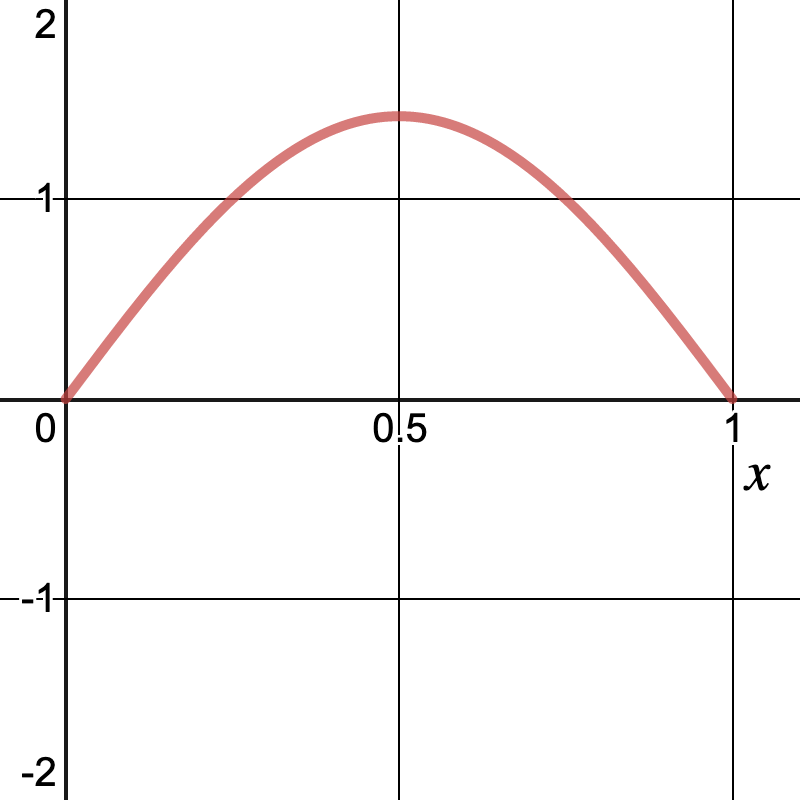
\includegraphics[width=\textwidth]{Figures_Part_2/state_1.png}
        \caption{$\psi_1(x)$.}
    \end{subfigure}
    ~ 
    \begin{subfigure}[h]{0.3\textwidth}
        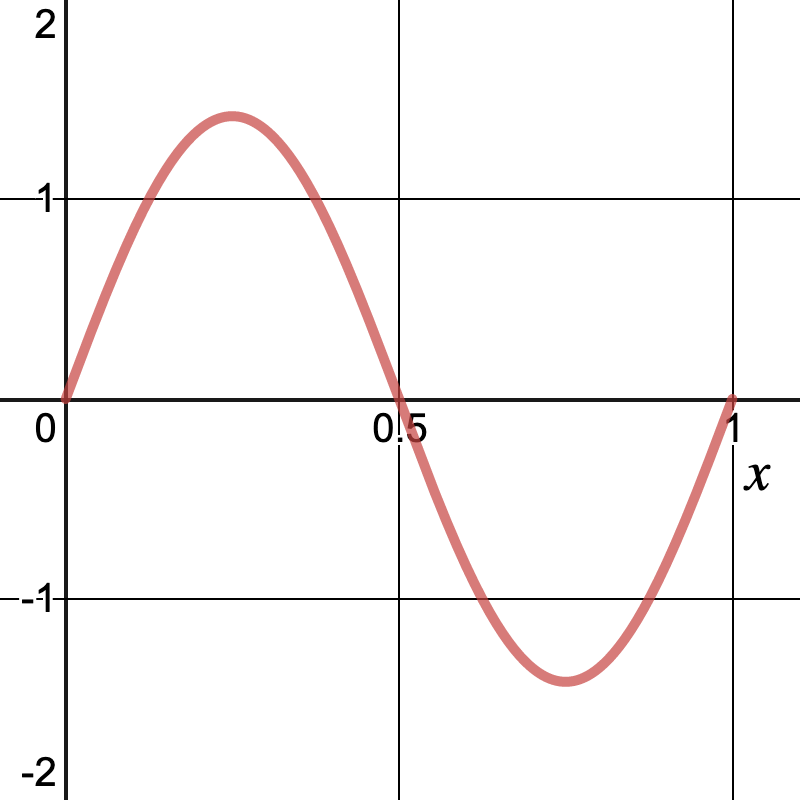
\includegraphics[width=\textwidth]{Figures_Part_2/state_2.png}
        \caption{$\psi_2(x)$.}
    \end{subfigure}
    ~
    \begin{subfigure}[h]{0.3\textwidth}
        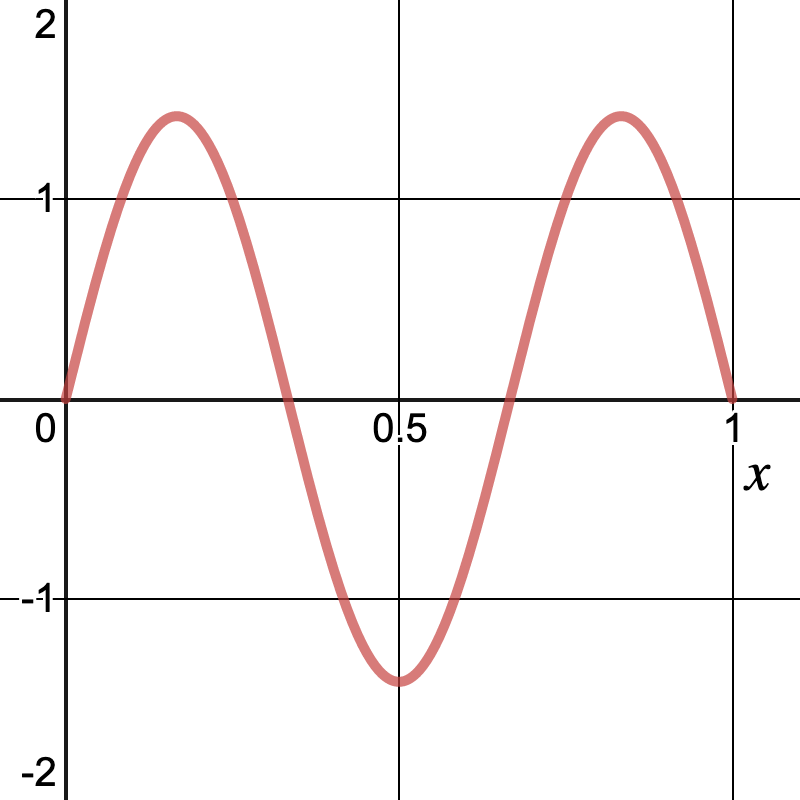
\includegraphics[width=\textwidth]{Figures_Part_2/state_3.png}
        \caption{$\psi_3(x)$.}
    \end{subfigure}\\
    
        \begin{subfigure}[h]{0.3\textwidth}
        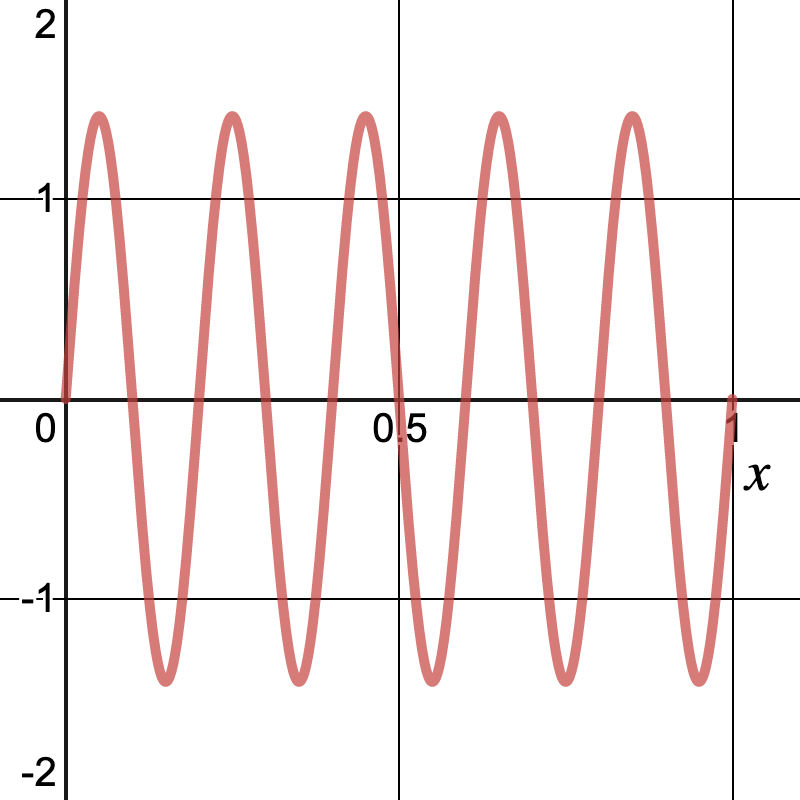
\includegraphics[width=\textwidth]{Figures_Part_2/state_10.png}
        \caption{$\psi_{10}(x)$.}
    \end{subfigure}
    ~ 
    \begin{subfigure}[h]{0.3\textwidth}
        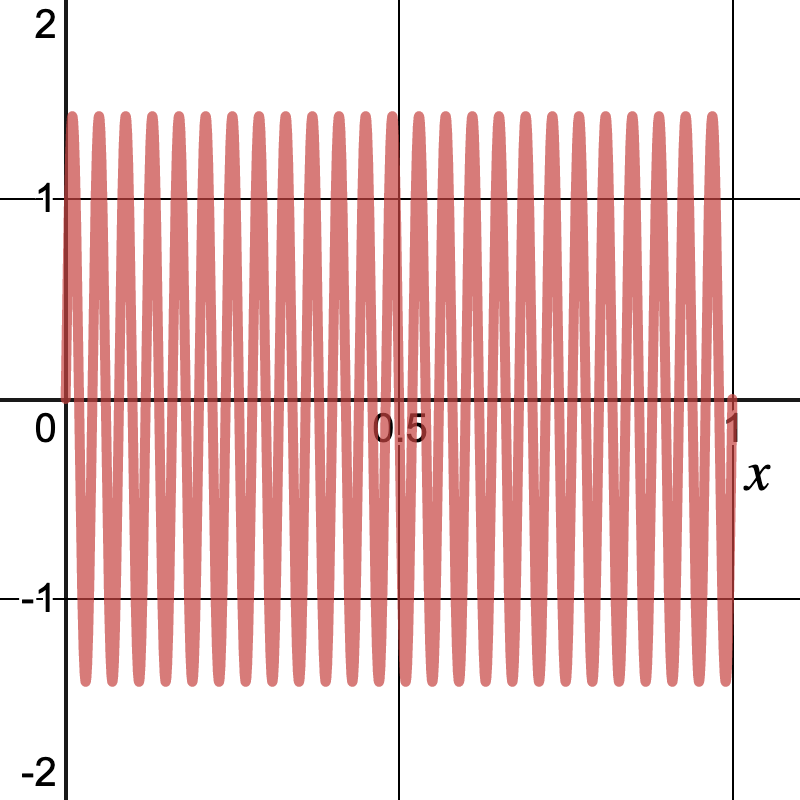
\includegraphics[width=\textwidth]{Figures_Part_2/state_50.png}
        \caption{$\psi_{50}(x)$.}
    \end{subfigure}
    ~
    \begin{subfigure}[h]{0.3\textwidth}
        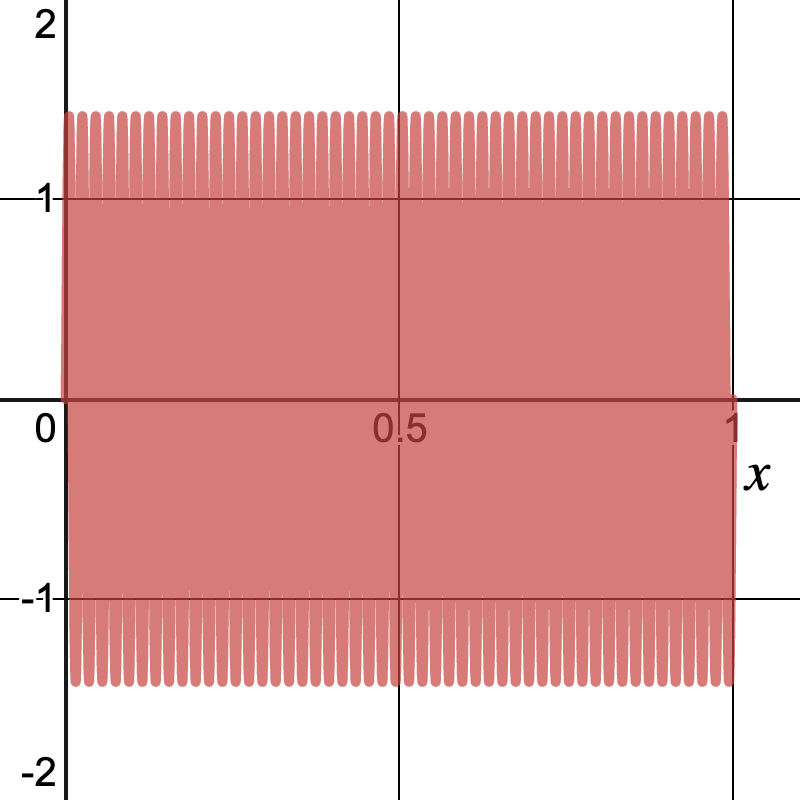
\includegraphics[width=\textwidth]{Figures_Part_2/state_100.png}
        \caption{$\psi_{100}(x)$.}
    \end{subfigure}
        \end{figure}

\noindent One may notice that as we allow for larger and larger $n$ values, the states seem to start to approach a uniform value on the region $[0,L]$. In fact, if we were to take the limit as $n\to \infty$, we would essentially have that $\psi_\infty(x) = \frac{1}{L}$ which would be equivalent to the case of a classic particle randomly placed in the box.

It is possible to prepare this system in a \boldgreen{superposition} by, for example, considering the wavefunction
\[
\Psi(x) = \frac{1}{\sqrt{2}}\left(\psi_1(x) + \psi_2(x)\right).
\]
In fact, due to the orthonormality of the states and the linearity of the Hamiltonian for the 1-dimensional box, we can write a wavefunction $\Psi(x)$ as
\[
\boxed{\Psi(x)=\sum_{j=1}^\infty a_j \psi_j(x) \qquad \textrm{where}\qquad \sum_{j=1}^\infty a_j^2 = 1.}
\]

\subsubsection{Summary of the 1-Dimensional Box}
\begin{itemize}
    \item The equation for the 1-Dimensional box is the same as the eigenfunctions of the Laplacian equation shown before. That is, we have $V(x)=0$ and we allow for $x$ to be in the range $[0,L]$ and get the equation
    \begin{align*}
        H\psi &= E \psi\\
        -\frac{\hbar^2}{2m}\frac{d^2}{dx^2}\psi = E \psi.
    \end{align*}
    \item We solved this equation as a second order linear equation and used the boundary values to determine possible solutions.  It turns out that we get a quantized set of solutions $\psi_n$ each corresponding to an energy level $E_n$. These energy levels were given by $E_n = \frac{n^2 \hbar^2 \pi^2}{2mL}$ and so the energies increase proportionally to $n^2$. We can see a plot of energies here.
    \begin{figure}[H]
        \centering
        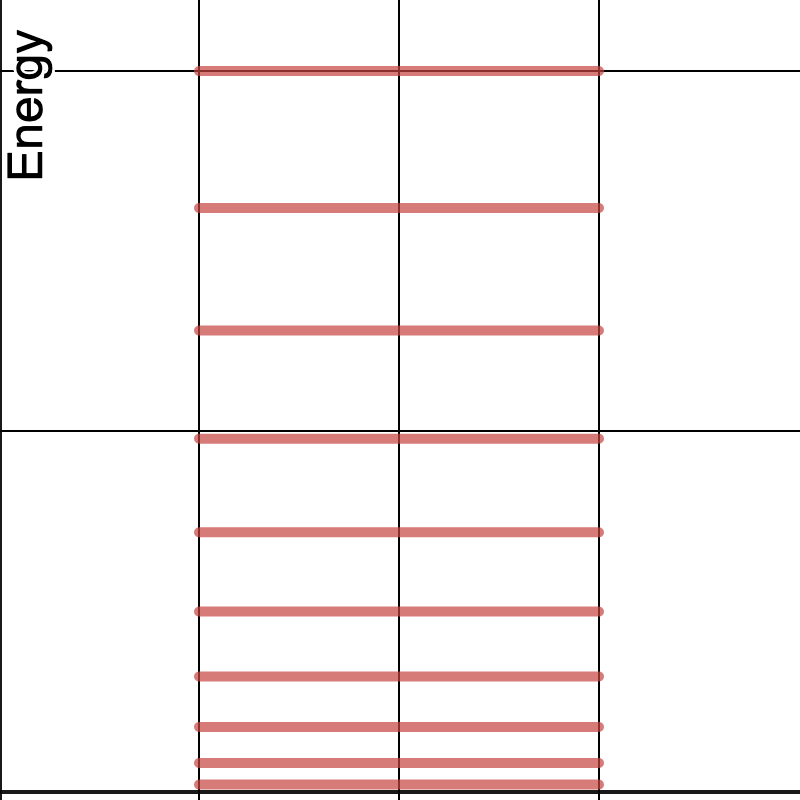
\includegraphics[width=.5\textwidth]{Figures_Part_2/energy_levels.png}
        \caption{Energy levels of the 1-dimensional box.}
    \end{figure}
    \item We normalized the solutions $\psi_n$ and found that they give rise to a probability function that describe the probability of a particle being in a region $[a,b]$. 
    \item Namely, we can take a wavefunction
    \[
    \Psi(x)=\sum_{j=1}^\infty a_j \psi_j(x)
    \]
    where $\sum_{j=1}^\infty a_j^2 = 1$. If more than one $a_j\neq 0$, then this wavefunction describes a superposition state. We can then find the probability of a particle with wavefunction $\Psi$ being in the region $[a,b]$ by
    \[
    P([a,b])=\int_a^b |\Psi(x)|^2dx.
    \]
    \item As we let $n\to \infty$, we recover the case of the classical particle.  We should expect this since we do not observe this odd quantum phenomenon on large scale!
\end{itemize}

\begin{exercise}
Look up common energies for something like throwing a baseball. Compare this to $E_n$ for $m=1[g]$ and $L=1[m]$. You will have to use the measured value for Planck's reduced constant
\[
\hbar \approx 1.0545718\cdot 10^{-34}[kg \cdot m^2 /s].
\]
\end{exercise}



\part{Elements of Analysis}
\chapter{Sequences and Series}
\section{Sequences}
The next stop for us is sequences and series.  In the realm of analysis, these are very important objects.  It turns out that they are rather useful in applied sciences as well.  Specifically, power series are undeniably useful.  However, to gain understanding for those series, we need to start at the beginning with sequences.  From there, we can realize a series as a sequence.  Finally, we can turn functions into series, which, believe it or not, gives us the ability to solve problems like differential equations or to approximate harder problems in a nicer way.

\begin{df}{Sequences}{sequences}
An (infinite) \boldgreen{sequence} $\{a_n\}_{n=1}^\infty$ is an (infinite) list of numbers typically written as follows:
\[
\{a_n\}_{n=1}^\infty = a_1,~ a_2,~ a_3, \cdots.
\]
While some speak of finite sequences, we will not.  All sequences we consider are infinite, and so we drop the extra adjective.
\end{df}

Sequences can come up in all types of ways.  For example, consider these two sequences related to the number $\pi$.  We can take
\[
a_n = \textrm{the $n^\textrm{th}$ digit of the number $\pi$}
\]
and so 
\[
\{a_n\}_{n=1}^\infty = 3,~1,~4,~1,~5, \dots.
\]
We could also consider a sequence that successively approximates $\pi$ as
\[
b_n = \textrm{the $n^\textrm{th}$ decimal approximation of $\pi$}
\]
which is
\[
\{b_n\}_{n=1}^\infty = 3,~3.1, ~ 3.14, ~ 3.141, ~ 3.1415, \dots.
\]

\subsection{Convergence}
When investigating series, we often care about whether they seem to trend towards a common value or not.  This can be rather hard to deal with in some cases.  But, the intuition on when a series converges is very important and shows up in various ways one should care about.  For example, we often use computer approximations for functions (since most functions cannot be exactly calculated with a computer) and we should know when these approximations are accurate and tend towards the exact function we desire.  This motivates the following definition.

\begin{df}{Convergence of a Sequence}{convergence_of_sequence}
Consider a sequence $\{a_n\}_{n=1}^\infty$.  We say that the sequence \boldgreen{converges} to its \boldgreen{limit} $L$ if for any number $\epsilon>0$ there exists $N\in \N$ such that for any $K\geq N$ we have
\[
|a_{K}-L|<\epsilon.
\]
We then write
\[
\lim_{n\to \infty} a_n = L
\]
or
\[
a_n \to L.
\]

If a sequence does not converge to any limit, then we say the sequence \boldgreen{diverges}.
\end{df}

Admittedly, this definition is a bit obtrusive.  What is it really saying?  Let's decode this a bit. Think of $\epsilon$ as a tolerance parameter (i.e., how accurate you would like a measurement to be) telling us how far from the ideal measurement $L$ we are. Then, what this definition is saying is that if we look far enough along in our sequence we can be as close to the ideal $L$ as we wish.  

\begin{ex}{Approximations with $\pi$}{approx_pi}
Consider the two sequences $\{a_n\}_{n=1}^\infty$ and $\{b_n\}_{n=1}^\infty$ we generated for $\pi$.  Which ones converge? Let us take a look first at
\[
\{a_n\}_{n=1}^\infty = 3,~1,~4,~1,~5, \dots.
\]
Note that this sequence, if we keep looking at successive digits, does not approach any single value.  In fact, if it did approach a single value it would have to approach a decimal $0,1,\dots, 9$.  Let's say that our sequence did converge to the decimal $0$. In which case our definition of convergence would imply that if we chose a tolerance of $0.5$, then at some point in our sequence we would have 
\[
|a_K - 0|=|a_n|=a_n<\epsilon=0.5,
\]
and so all $a_n$ after some point must be equal to $0$.  But, if that was the case, then $\pi$ would not have an infinite decimal expansion! And if we had chosen another decimal, this would still mean that $\pi$ is a rational number (which we can prove it is not). Hence, $a_n$ does not converge.

Considering $\{b_n\}_{n=1}^\infty$ may be a bit easier.  We designed this sequence to continually approximate $\pi$ as we put
\[
\{b_n\}_{n=1}^\infty = 3,~3.1, ~ 3.14, ~ 3.141, ~ 3.1415, \dots.
\]
One should believe then that $b_n\to \pi$.  We can test this with our definition.  Say we let $\epsilon = 0.1$, then we want
\[
|b_K-\pi|<\epsilon = 0.1.
\]
Now, $b_n$ is defined to be the $n^\textrm{th}$ approximation of $\pi$, so if we choose $N=2$, then for $K\geq N=2$, $b_K$ has at least the first two digits of $\pi$ correctly approximated.  Then
\[
|b_K - \pi| \leq |0.0415\dots | < 0.1 = \epsilon.
\]
Similarly, we could choose $\epsilon = 0.01$ and let $N=3$.  
\end{ex}

Often we want to define sequences in a functional way.  That is, we like to specify what the $n^\textrm{th}$ term of the sequence is by a function of $n$, $f(n)$. This is typically how sequences appear and it makes working with the definition of convergence a bit more simple as we can use rules from limits that we already know.

\begin{ex}{A Sequence Given by a Function}{sequence_by_funct}
Consider the sequence $\{a_n\}_{n=1}^\infty$ where 
\[
a_n = f(n) = \frac{1}{n}.
\]
We can then write out the sequence
\[
\{a_n\}_{n=1}^\infty = 1, ~\frac{1}{2}, ~\frac{1}{3}, ~ \frac{1}{4}, \dots.
\]
It seems like numbers in this sequence get smaller and smaller in magnitude, but are never negative.  So, one may guess that $\lim_{n\to \infty} a_n = 0$.  Let us prove that this is true.  Fix some $\epsilon >0$, then we want to find an $N$ so that for all $K\geq N$ we have
\[
|a_K - 0| = |a_K|=a_K<\epsilon.
\]
Now, we have that
\[
a_K=\frac{1}{K} < \epsilon
\]
which we can rearrange 
\begin{align*}
    \frac{1}{K} & < \epsilon \\
    \iff~ \frac{1}{\epsilon} & < K.
\end{align*}
Hence, if we pick a $N\geq K>\frac{1}{\epsilon}$ we guarantee that we satisfy our tolerance condition. Thus, since we found values of $N$ that satisfy a generic tolerance condition, we know that $a_n \to 0$.

We can see a picture of what is going on here.  I'll put the $\epsilon$ as a solid red line, and graph the points $a_N$ versus $N$ as $(N, a_N)$.
        \begin{figure}[H]
    \centering
    \begin{subfigure}[h]{0.3\textwidth}
        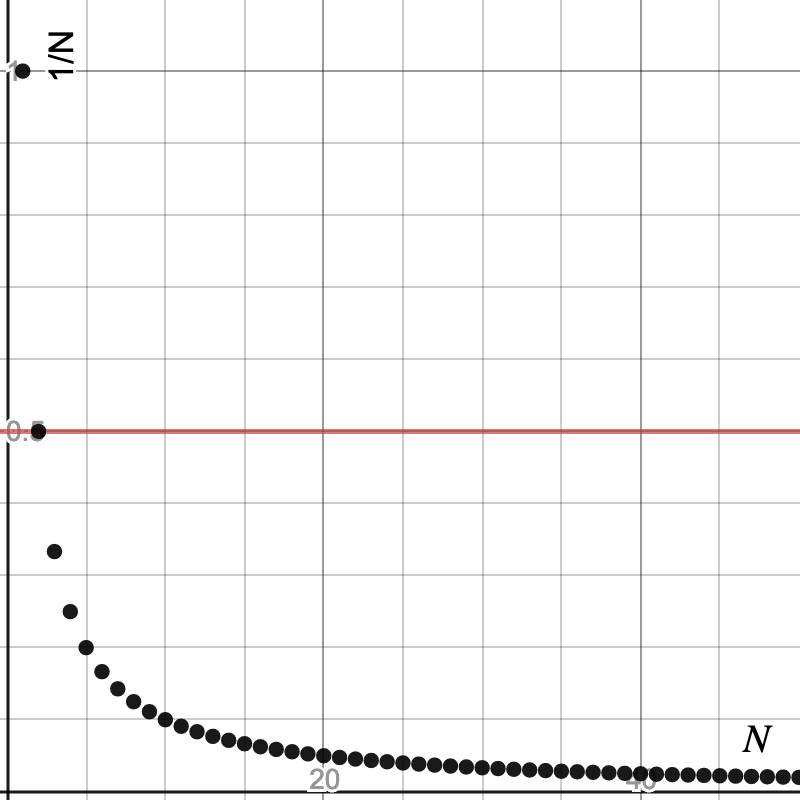
\includegraphics[width=\textwidth]{Figures_Part_3/tolerance_epsilon=05.png}
        \caption{$\epsilon=0.5$.}
    \end{subfigure}
    ~ 
    \begin{subfigure}[h]{0.3\textwidth}
        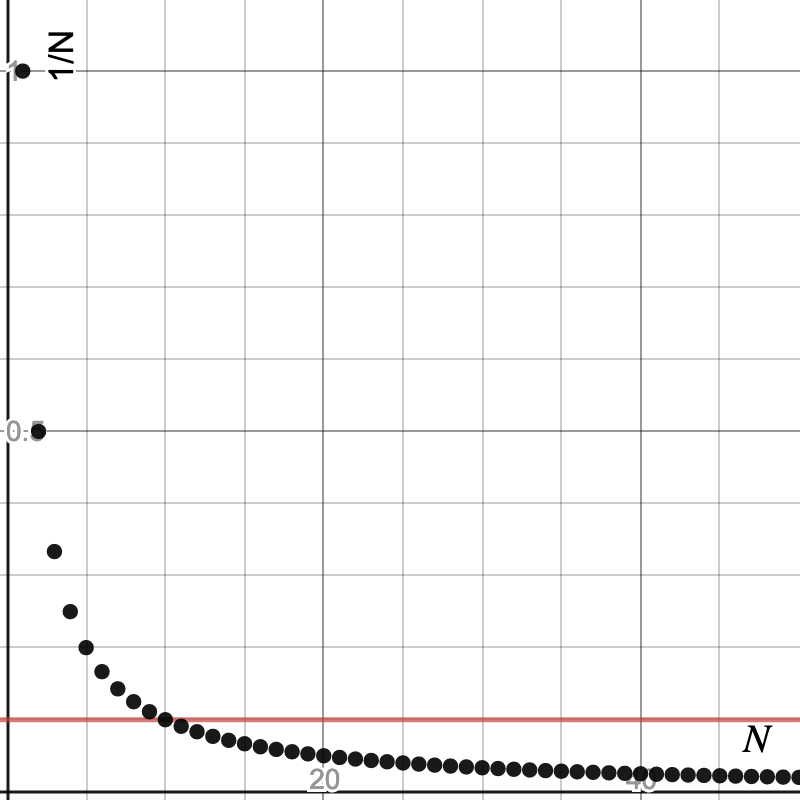
\includegraphics[width=\textwidth]{Figures_Part_3/tolerance_epsilon=01.png}
        \caption{$\epsilon=0.1$.}
    \end{subfigure}
    ~
    \begin{subfigure}[h]{0.3\textwidth}
        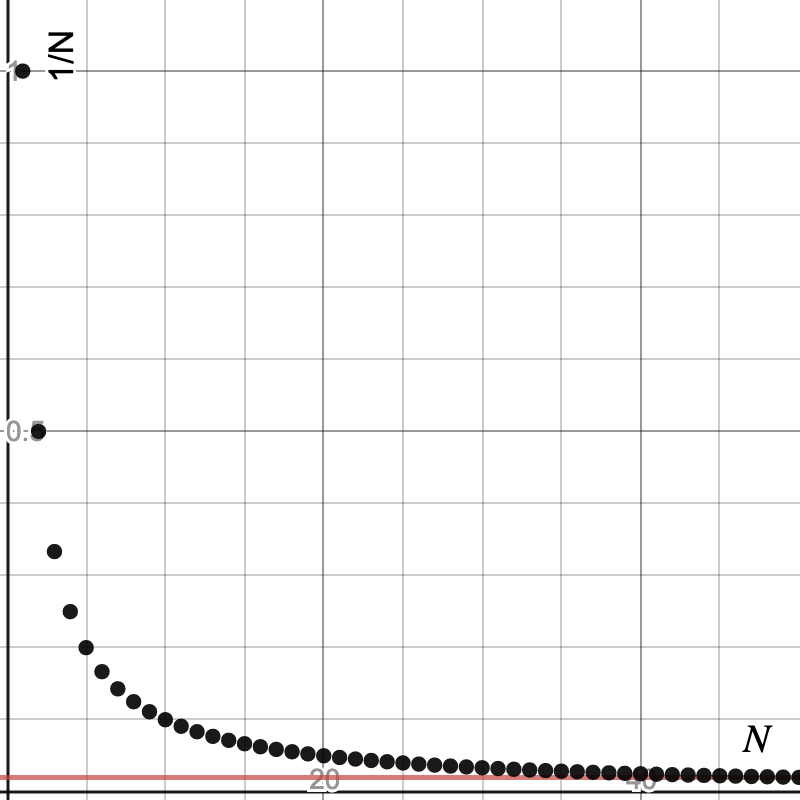
\includegraphics[width=\textwidth]{Figures_Part_3/tolerance_epsilon=002.png}
        \caption{$\epsilon=0.02$.}
    \end{subfigure}

        \end{figure}
\end{ex}

This definition of convergence is essentially the exact same definition as what we have seen for functions converging to their limit.  Hence, all the results we have on functions extends to this case.  This is why we wish to work with sequences defined by functions $f(n)$.  

\begin{prop}{Limit of Functions Gives the Limit for a Sequence}{limit_function_sequence}
Consider a sequence $\{a_n\}_{n=1}^\infty$ with $a_n = f(n)$.  Then the sequence converges to $L$ if and only if $\lim_{n\to \infty} f(n) = L$.
\end{prop}

Here's a short list of some limits you should feel free to use. 
        \begin{table}[H]
        \centering
        \renewcommand{\arraystretch}{1.75}
            \begin{tabular}{c|c}
                Function for $a_n$ &  Limit $\lim_{n\to \infty} a_n$\\
                \hline
                $a^n$ & $\begin{cases} 0 & \textrm{if $|a|<1$}\\ 1 & \textrm{if $a=1$} \\ \textrm{Diverges} &\textrm{otherwise}\end{cases}$\\
                \hline
                $n^p$ & $\begin{cases} 0 &\textrm{if $p\leq0$} \\ \textrm{Diverges} & \textrm{if $p>0$}\end{cases}$
            \end{tabular}
    \end{table}

It should be noted that not all sequences diverge in the same way.  Let us see this with an example of two different cases.

\begin{ex}{Different Ways of Diverging}{diff_diverging}
Consider the sequences $\{a_n\}_{n=1}^\infty$ and $\{b_n\}_{n=1}^\infty$ given by
\[
a_n = (-1)^n \qquad \textrm{and} \qquad b_n = n.
\]
We can write out the first few terms of each series
\begin{align*}
    \{a_n\}_{n=1}^\infty &= -1,~1,~-1,~1,~-1,~1,\dots\\
    \{b_n\}_{n=1}^\infty &= 1,2,3,4,5,6,\dots.
\end{align*}
Notice that $\{a_n\}_{n=1}^\infty$ never settles to a specific value as it just oscillates between $-1$ and $1$ indefinitely.  For $\{b_n\}_{n=1}^\infty$ we see that this sqeuence grows as $n$ grows. We sometimes add that $\{b_n\}_{n=1}^\infty$ \boldgreen{diverges to infinity}. If we took $c_n=-n$, we would have that $\{c_n\}_{n=1}^\infty$ \boldgreen{diverges to minus infinity}.
\end{ex}

Another way to describe a sequence converging is to show that the difference between successive values (i.e., differences between $a_N$ and $a_{N+1}$) get arbitrarily small.  Let us write this as a theorem. We'll define one term in this theorem as well.

\begin{thm}{Cauchy Sequences Converge}{cauchy_seq_converge}
Let $\{a_n\}_{n=1}^\infty$ be a sequence satisfying that for any $\epsilon >0$ there exists $N\in \N$ such that for $K\geq N$ we have
\[
|a_{K}-a_{K+1}|<\epsilon.
\]
We call such a sequence $\{a_n\}_{n=1}^\infty$ a \boldgreen{Cauchy sequence}.  Then if $\{a_n\}_{n=1}^\infty$ is a real (or complex) valued Cauchy sequence, then it is also convergent.
\end{thm}

\noindent This fact will become useful later on when we study series as it leads us to the comparison test.

\subsection{Recursive Sequences}

Some sequences we will see are defined in a \emph{recursive} way.  Meaning that instead of supplying a function for the terms (i.e., $a_n = f(n)$), we tend to start with an initial term $a_1$ and define future terms based on that.  For example, we could define a sequence $\{a_n\}_{n=1}^\infty$ by
\[ 
a_1 = 1 \qquad \textrm{and} \qquad a_n = \frac{1}{2} a_{n-1}.
\]
From this definition, we can find that
\[
a_2 = \frac{1}{2} a_1 = \frac{1}{2} \cdot 1 = \frac{1}{2},
\]
and
\[
a_3 = \frac{1}{2} a_2 = \frac{1}{2} \cdot \frac{1}{2} = \frac{1}{4}.
\]
If we continued on, we could write out the sequence as
\[
\{a_n\}_{n=1}^\infty = 1, \frac{1}{2},\frac{1}{4}, \frac{1}{8}, \dots.
\]
When we define a sequence in this way, we call it \boldgreen{recursive}.

\begin{ex}{Fibonacci Sequence}{fib_seq}
One very important recursive sequence is the \boldgreen{Fibonacci sequence} $\{F_n\}_{n=1}^\infty$ defined by summing up the previous two terms in the sequence to get the new one.  That is, we can define
\[
F_1 = 0, \qquad F_2=1, \qquad \textrm{and} \qquad F_n = F_{n-1} + F_{n-2}.
\]
We can write the first few terms in this sequence by following the above rule with the initial values for $F_1$ and $F_2$ to get
\[
\{F_n\}_{n=1}^\infty = 0,1,1,2,3,5,8,13,21,34,\dots.
\]
This sequence shows up in many natural systems! 
\end{ex}

\begin{exercise}
Look up where this Fibonacci sequence shows up in nature.
\end{exercise}

\section{Series}

What else can we do with sequences? Well, instead of just keeping a sequence $\seqan$ as a list of numbers, we could consider operations with these infinitely many numbers.  For example, we could add the numbers as
\[
\sum_{n=1}^\infty a_n = a_1 + a_2 + a_3 + \cdots
\]
or even multiply them
\[
\prod_{n=1}^\infty a_n = a_1\cdot a_2 \cdot a_3 \cdots.
\]
In our case, we will care about adding up terms in a sequence. 

\begin{df}{Series}{series}
Given a sequence $\seqan$ we can create an (infinite) \boldgreen{series}
\[
\sum_{n=1}^\infty a_n.
\]
\end{df}

What does it really mean to add up infinitely many numbers? Can this even be a finite result? It turns out that both of these questions can be answered at the same time.  If we rethink what we are doing a bit, it turns out that we need no other definition than convergence of a sequence.  Our goal now is to make a series into a sequence, and we will see how we can make sense of this infinite sum.

Consider a series $A=\sum_{n=1}^\infty a_n$.  We can then consider \boldgreen{partial sums} of the series by looking at finite approximations to the infinite sum.  That is, the $N^\textrm{th}$ partial sum is given by
\[
A_N = \sum_{n=1}^N a_n = a_1 + a_2 + a_3 + \cdots + a_N.
\]
Now, we can collect all of the partial sums $A_1,A_2,A_3,\dots$ and notice that this creates a sequence $\seqAn$.  

\begin{df}{Convergence of a Series}{convergence_series}
Given a series $\displaystyle{\serA}$ and the sequence of partial sums $\seqAn$. We say that the series $\serA$ \boldgreen{converges} to $A$ if the sequence of partial sums converges to $A$ and put
\[
A = \serA.
\]
If the series does not converge, we say that it \boldgreen{diverges}.
\end{df}

\begin{remark}
We should note that a series $\serA$ cannot converge if the sequence $\seqan$ does not converge to zero!
\end{remark}

\begin{ex}{Series Approximation of $\pi$}{series_approx_pi}
Previously, we had the sequences
\[
\seqan = 3,~1,~4,~1,~5, \dots
\]
and
\[
\seqbn = 3,~3.1,~3.14,~3.141,~3.1415,\dots
\]
that we used to build up the number $\pi$.  It turns out we can relate these two sequences in the following way.  Consider the series
\begin{align*}
\sum_{n=1}^\infty 10^{-n+1} a_n &= 3+0.1+0.04+0.001+0.0005+\cdots.
\end{align*}
Note, we are adding numbers of smaller and smaller magnitude. Now, notice if we take the sequence of partial sums, we find that we get back the sequence $\seqbn$
\[
b_N = \sum_{n=1}^N 10^{-n+1}a_n
\]
Since we worked with the sequence $\seqbn$ previously, we know that we have $b_n\to \pi$ and thus the series converges to $\pi$ as well
\[
\pi = \sum_{n=1}^\infty 10^{-n+1}a_n.
\]
\end{ex}

We are often provided each element of a sequence by a function. That is, $a_n=f(n)$.  If this is the case for terms in a series as well, it turns out we can use other means to show a series converges.  Let us consider the following series.

\begin{ex}{Geometric Series}{geo_series}
Consider a sequence defined by $a_n = ar^n$.  Then we call the following a \boldgreen{geometric series}
\[
\sum_{n=1}^\infty = \sum_{n=1}^\infty ar^n
\]
In order for the series to converge, we must have that the sequence $a_n \to 0$.  This means that we must have $|r|<1$ as if $|r|<1$ then $\lim_{n\to \infty} a_n =0$. If this is the case, then we can take our series
\[
\sum_{n=1}^\infty ar^n = a\sum_{n=1}^\infty r^n = a(r+r^2+r^3+\cdots).
\]
So the $N^\textrm{th}$ partial sum is
\[
A_{N} = a(r+r^2+r^3+\cdots+r^{N}).
\]
Then we can subtract $rA_N$ from both sides
\begin{align*}
A_N - rA_N &= a(r+r^2+r^3+\cdots+r^N) - a(r^2+r^3+r^4+\cdots+r^{N+1})\\
 (1-r)A_N&=a(r-r^{N+1})\\
 A_N &= a\left( \frac{r-r^{N+1}}{1-r}\right).
\end{align*}
Now consider the limit for the sequence of partial sums
\begin{align*}
\lim_{N\to \infty} A_N &= \lim_{N \to \infty} a\left(\frac{r-r^{N+1}}{1-r}\right)\\
&=\frac{ar}{1-r}.
\end{align*}
Thus, we have that the geomnetric series converges
\[
\boxed{\sum_{n=1}^\infty ar^n = \frac{ar}{1-r}.}
\]
\end{ex}

Now, not only have we shown that a whole set of series converges, but we have found what they converge to! And, as it turns out, geometric series show up quite often.  We can use our formula to find the sum of following series.

\begin{ex}{A Specific Geometric Series}{specific_geometric_series}
Consider the geometric series
\[
\sum_{n=1}^\infty \frac{1}{2^n}.
\]
Note that this is a geometric series with $a=1$ and $r=\frac{1}{2}$ as we can write the series as
\[
\sum_{n=1}^\infty a r^n = \sum_{n=1}^\infty 1\cdot \left( \frac{1}{2}\right)^n.
\]
Our formula says that
\[
\sum_{n=1}^\infty ar^n = \frac{ar}{1-r}
\]
and hence we can plug in for both $a$ and $r$ to see
\[
\boxed{\sum_{n=1}^\infty \frac{1}{2^n}=\frac{1/2}{1-1/2}=1.}
\]
\end{ex}

How about convergence for other types of series? There is a test that we can perform that will tell us more information.  We call this test the \boldgreen{ratio test}. However, the ratio test won't be a test that tells us if \emph{any} series converges or diverges.

\begin{prop}{Ratio Test}{ratio_test}
Consider the series $\serA$. If we have that 
\[
L=\lim_{n\to \infty}\left| \frac{a_{n+1}}{a_n}\right|<1,
\]
then the series converges (absolutely).  If $L>1$, then the series diverges.  If $L=1$, then we gain no information.
\begin{proof}
First, if $L>1$, then each term is growing in magnitude for this series, and thus $a_n\not\to 0$ and the series cannot converge.

If $L<1$, then at some point along our series, $N\in \N$, we have that $1>r>\left| \frac{a_{n+1}}{a_n}\right|$
\begin{align*}
\sum_{n=1}^\infty |a_n| &= \sum_{n=1}^N |a_n| + \sum_{j=N}^\infty |a_j|\\
&= A_N + \sum_{j=1}^\infty |a_{N+j}|\\
&< A_N + \sum_{j=1}^\infty r^j |a_{N+1}|\\
&= A_N +|a_{N+1}| \sum_{j=1}^\infty r^j\\
&= A_N + \frac{|a_{N+1}|r}{1-r}<\infty.
\end{align*}
Hence the series converges (absolutely).
\end{proof}
\end{prop}

\begin{remark}
A series $\serA$ \boldgreen{converges absolutely} if 
\[
\sum_{n=1}^\infty |a_n| 
\]
converges.
\end{remark}

The ratio test is a helpful tool, but it does have its shortcomings.  We can take a look at an example where the test tells us pertinent information and one where it does not.  

\begin{ex}{Series for $e$}{series_for_e}
One can actually define the number $e$ by the series
\[
e=\sum_{n=0}^\infty \frac{1}{n!}
\]
where $n!$ is the factorial function 
\[
n!=n\cdot (n-1)\cdot (n-2)\cdots 2\cdot 1
\]
and we define $0!=1$.  Now, by saying the series above equals $e$, we should think that the series converges. But we can prove this is true using the ratio test.  Consider the terms
\[
a_n = \frac{1}{n!} \qquad \textrm{and} \qquad a_{n+1}=\frac{1}{(n+1)!}=\frac{1}{(n+1)n!}.
\]
Then if we consider
\begin{align*}
    \lim_{n\to \infty} \left| \frac{a_{n+1}}{a_n}\right|&= \lim_{n\to \infty} \left| \frac{\frac{1}{(n+1)n!}}{\frac{1}{n!}}\right|\\
    &= \lim_{n\to \infty } \left| \frac{n!}{(n+1)n!}\right|\\
    &= \lim_{n \to \infty} \left| \frac{1}{n+1}\right|\\
    &= 0.
\end{align*}
Hence, by the ratio test with $L<1$, we know the series converges. And as stated above, it converges to Euler's number $e$.
\end{ex}

Below is an important class of series called \emph{$p$-series}. These and geometric series are some of the most common that we will see.  It turns out that some $p$-series converge and others diverge depending on the value for $p$. However, the ratio test gives us no information on any of them.

\begin{ex}{$p$-Series}{}
Consider a general $p$-series which has the form
\[
\sum_{n=1}^\infty \frac{1}{n^p}
\]
where $p$ can be any real number. Now, if $p\leq 0$, then we have
\[
\lim_{n \to \infty} \frac{1}{n^p}>0
\]
and the series cannot possibly converge.  However, with the ratio test for any $p$, we see that
\[
\lim_{n\to \infty} \left|\frac{a_{n+1}}{a_n}\right|=\lim_{n\to \infty} \left|\frac{\frac{1}{(n+1)^p}}{\frac{1}{n^p}}\right|  = \lim_{n\to \infty} \left| \frac{n^p}{(n+1)^p}\right| = 1.
\]
So, for any value of $p$, the ratio test tells us nothing.  However, we can show that the $p$-series does converge for certain values of $p$.
\end{ex}

\begin{exercise}
Investigate the limit in the ratio test 
\[
\lim_{n\to \infty} \left|\frac{\frac{1}{(n+1)^p}}{\frac{1}{n^p}}\right|
\]
in more detail to show that it indeed is equal to one.
\end{exercise}

There is another test we can use to determine convergence of series which will work in some cases when the ratio test does not. We call this the \boldgreen{integral test}.

\begin{prop}{Integral Test}{integral_test}
Consider the series $\sum_{n=N}^\infty$ with $a_n=f(n)$.  Then the series converges if and only if
\[
\int_{N}^\infty f(x)dx
\]
is finite. If the integral diverges, the series does as well. \emph{Note, the integral is likely not equal to the series. It only tells us whether the series converges or not!}
\end{prop}

\begin{ex}{$p$-Series Integral Test}{int_test_p_series}
Going back to the $p$-series, we need to check whether for $p>0$ the series converges as we already ruled out $p\leq 0$ cannot.  So our series in question is
\[
\sum_{n=1}^\infty \frac{1}{n^p}
\]
so our $f(n)=\frac{1}{n^p}$ and our $N=1$.  Thus we investigate the integral
\[
\int_1^\infty \frac{1}{x^p}dx.
\]
Now, if $0<p<1$, then we have
\begin{align*}
    \int_1^\infty \frac{1}{x^p}dx &= \left[\frac{1}{-p+1} x^{-p+1} \right]_1^\infty\\
    &= \infty,
\end{align*}
since $-p+1>0$ and so $x^{-p+1}$ approaches infinity as $x\to \infty$ and this integral diverges.  Hence, the $p$-series also diverges for $0<p<1$. 

For $p=1$, we find that the integral is
\[
\int_1^\infty \frac{1}{x} dx = \left[ \ln(x) \right]_1^\infty
\]
and $\ln(x)\to \infty$ as $x\to \infty$ so this integral diverges as well.  

For $p>1$, we have
\[
\int_1^\infty \frac{1}{x^p}dx = \left[ \frac{1}{-p+1}x^{-p+1}\right]_1^\infty
\]
where $-p+1<0$. Thus, in this case, $x^{-p+1}\to 0$ as $x\to \infty$ and this integral is finite!  So, we have the following result.
\[
\sum_{n=1}^\infty \frac{1}{n^p} \qquad \begin{cases} \textrm{Diverges} & \textrm{if $p\leq 1$} \\
\textrm{Converges} & \textrm{if $p>1$}\end{cases}.
\]
\end{ex}

One last useful test is to compare to series we know more about. We call this the \boldgreen{comparison test}

\begin{prop}{Comparison Test}{comparison_test}
Suppose that we have two series $\sum_{n=N_1}^\infty a_n$ and $\sum_{n=N_2}^\infty b_n$ with $a_n,b_n\geq 0$ and for some $N \in \N$ we have that for all $K\geq N$ that $a_n\leq b_n$. Then
\begin{itemize}
    \item If $\sum_{n=N_2}^\infty b_n$ is convergent, then so is $\sum_{n=N_1}^\infty a_n$.
    \item If $\sum_{n=N_1}^\infty a_n$ is divergent, then so is $\sum_{n=N_2}^\infty b_n$.
\end{itemize}
\end{prop}


\chapter{Power Series}
Since we have constructed different sequences and series, we can move forward into making them more useful for us.  The biggest use for series in our case will be to try and think of functions as a series. Specifically, we may be able to represent a function as a \emph{power series}.  This has many advantages! For one, we can differentiate and integrate a series term by term which simplifies calculations immensely.  Another advantage is the ability to approximate complicated functions.  This is especially useful if one ever plans to use a computer to perform computations.  

\section{Power Series}

Formally, a \boldgreen{power series} is a series with a variable $x$ (typically $x\in \R$ or $z\in \C$) written as
\[
\sum_{n=0}^\infty a_n x^n \qquad \textrm{or} \qquad \sum_{n=0}^\infty a_n z^n.
\]
An immediate question is whether or not this series converges and if that convergence depends on the choice of $x$ we are inputting into the expression.  The tools from the previous chapter allow us to determine this.  But, before that, it is important to get a little intuition on what we're doing here.

A power series is much like a polynomial function
\[
p(x) = a_0 + a_1 x + a_2 x^2 + \cdots + a_N x^N
\]
except for that a power series continues on indefinitely. That is, there is no highest power of $x$ for a power series!  However, if we consider a partial sum of a power series we can realize that as a polynomial. For example, using the series above the $N^\textrm{th}$ partial sum is equivalent to the polynomial above
\[
p(x)=\sum_{n=0}^N a_n x^n.
\]
So, a finite part of a power series is just a polynomial.  In all honesty, this is essentially the idea behind the construction to a power series.  We tend to build these power series as polynomial approximations to functions we already know, or use power series to determine functions in a new way.

\begin{ex}{Partial Sums for Power Series}{partial_sum_power_series}
Consider the power series with $a_n = \frac{1}{n!}$. We write this as
\[
\sum_{n=0}^\infty \frac{x^n}{n!}.
\]
This is an extremely important power series as we will repeatedly.  We can also write this series as
\[
\sum_{n=0}^\infty \frac{x^n}{n!} = 1 + x + \frac{x^2}{2}+\frac{x^3}{6}+\cdots.
\]
Now, let us take the following partial sums and see what the graphs look like. 
\begin{align*}
    \sum_{n=0}^0 \frac{x^n}{n!} &= 1\\
    \sum_{n=0}^1 \frac{x^n}{n!} &= 1+x\\
    \sum_{n=0}^6 \frac{x^n}{n!} &= 1+x+\frac{x^2}{2}+\frac{x^3}{6}+\frac{x^4}{24}+\frac{x^5}{120}+\frac{x^6}{720}.
\end{align*}
Notice how terms of higher powers of $x$ have increasingly smaller contributions to the sum as the denominator gets larger and larger. Below are plots of these.
\begin{figure}[H]
\centering
    \begin{subfigure}[h]{.3\textwidth}
        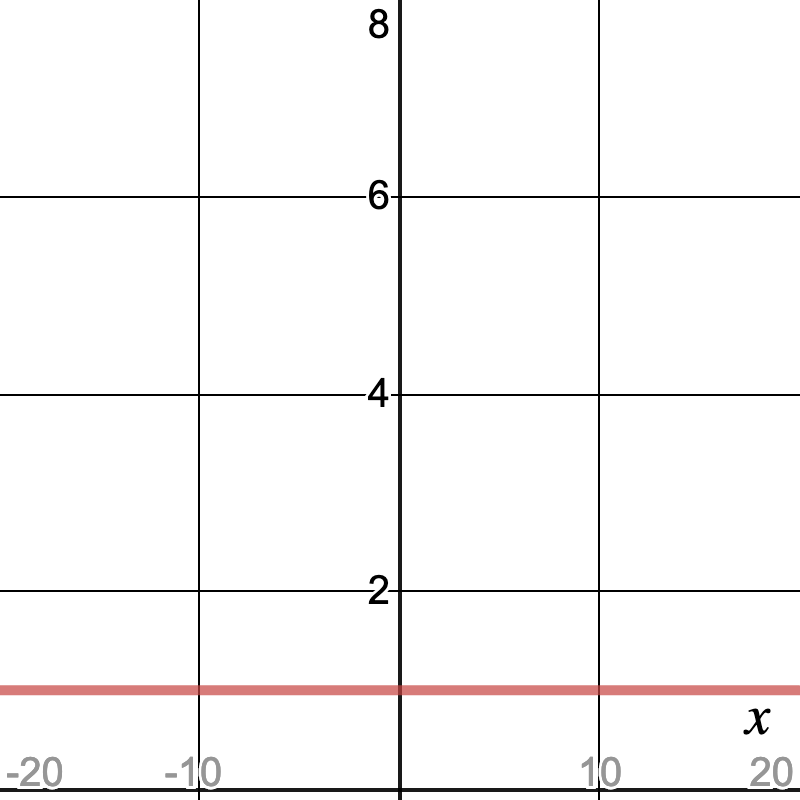
\includegraphics[width=\textwidth]{Figures_Part_3/ex_powseries_N=0.png}
        \caption{Partial sum with $N=0$.}
    \end{subfigure}
    ~
    \begin{subfigure}[h]{.3\textwidth}
        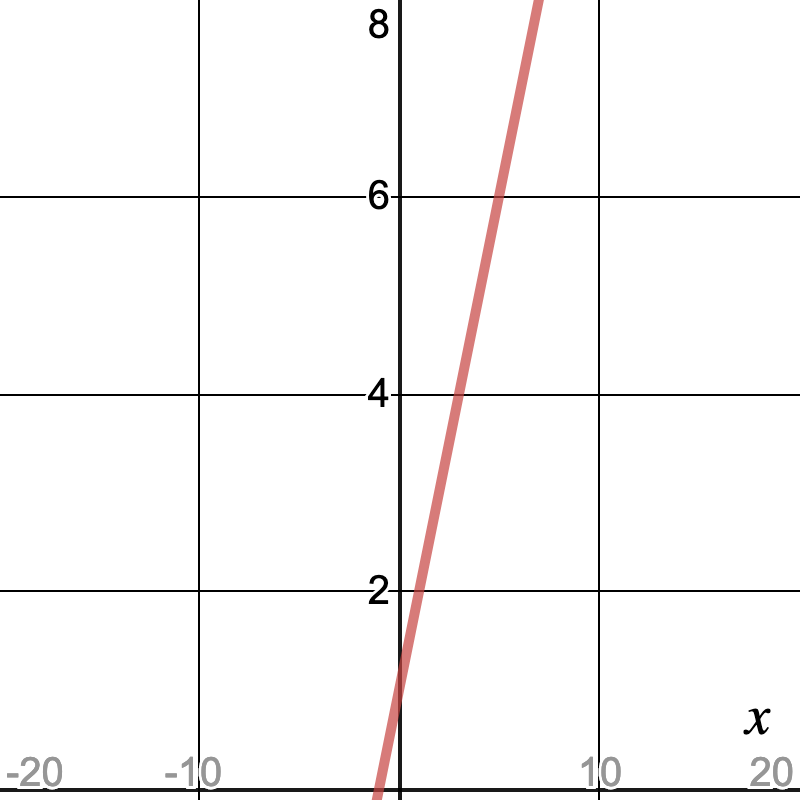
\includegraphics[width=\textwidth]{Figures_Part_3/ex_powseries_N=1.png}
        \caption{Partial sum with $N=1$.}
    \end{subfigure}
    ~
    \begin{subfigure}[h]{.3\textwidth}
        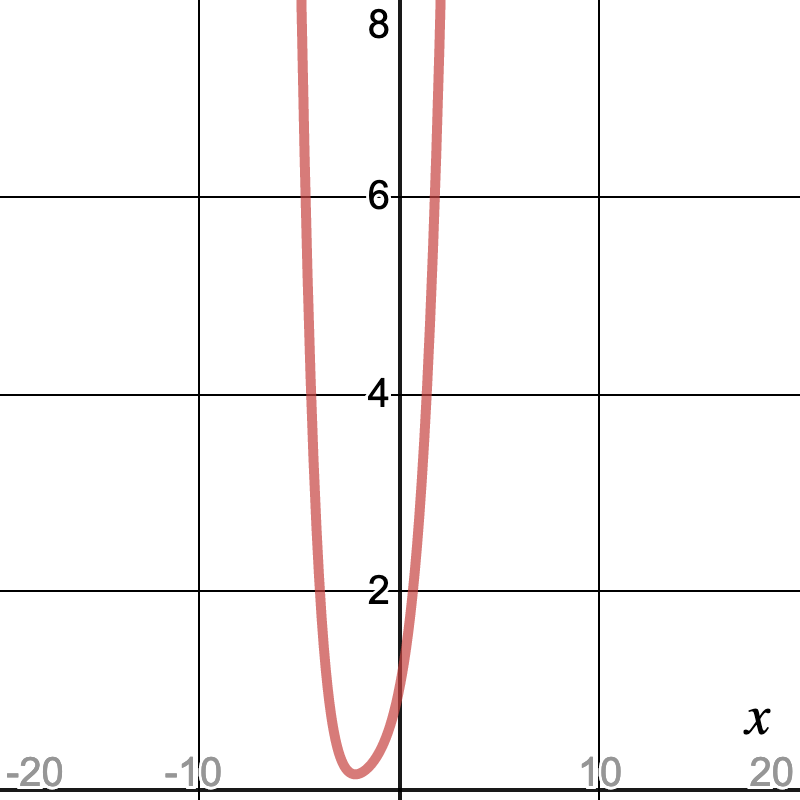
\includegraphics[width=\textwidth]{Figures_Part_3/ex_powseries_N=6.png}
        \caption{Partial sum with $N=6$.}
    \end{subfigure}
\end{figure}
\end{ex}

Before we carry on and see this used in a more applicable way, we just need to know how to talk about convergence of a power series.  A power series is no different than a series, it's just that there is a variable input that may affect convergence.  For example, for large $n$, if $x$ is large, then $x^n$ will be very large.  Thus we must have that the denominator in each term of the power series also grows rapidly. We can test this with the ratio test and determine the values of $x$ (or even $z\in \C$) in which the series converges.

\begin{df}{Radius of Convergence}{radius_of_convergence}
Consider a power series given by $\sum_{n=0}^\infty a_n x^n$.  We define the \boldgreen{radius of convergence} to be the largest value for $|x|$ such that
\[
\lim_{n\to \infty} \left| \frac{a_{n+1}x^{n+1}}{a_n x^n}\right| < 1.
\]
\end{df}

In the above definition we simply used the ratio test to define this. One should also note that this can be generalized slightly to allow for complex valued input $z\in \C$.  All that has to be done is to exchange the absolute value for the modulus.

\begin{ex}{Infinite Radius of Convergence}{radius_of_conv_ex}
Consider again the power series $\sum_{n=0}^\infty \frac{x^n}{n!}$. We wish to find the radius of convergence.  So consider the limit
\begin{align*}
    \lim_{n\to \infty} \left| \frac{\frac{x^{n+1}}{(n+1)!}}{\frac{x^n}{n!}}\right|&= \lim_{n\to \infty} \left| \frac{x}{n+1}\right|\\
    &= 0.
\end{align*}
Since $x$ does not factor into this limit, it does not matter what values of $x$ we plug in. That is, the series will converge no matter our choice for $x$. Fundamentally, this is because $n!$ grows rapdily even compared to $x^n$. Thus, the radius of convergence is infinite.
\end{ex}

\begin{ex}{Finite Radius of Convergence}{radius_of_conv_ex2}
Consider the power series
\[
\sum_{n=1}^\infty \frac{x^n}{n} = x + \frac{x^2}{2}+\frac{x^3}{3}+\frac{x^4}{4}+\cdots.
\]
This power series is similar to a $p$-series for $p=1$.  Hence, we know that if we take $x=1$, the series does not converge.  However, one should note that
\[
\sum_{n=1}^\infty \frac{(-1)^n}{n} = \ln(2).
\]
Given that, we should expect this series to converge for some values of $x$. So, let us use our ratio test 
\begin{align*}
    \lim_{n\to \infty} \left| \frac{\frac{x^{n+1}}{n+1}}{\frac{x^n}{n}}\right| &= \lim_{n\to \infty} \left| \frac{nx}{n+1} \right|\\
    &= |x| \cdot \lim_{n\to \infty} \frac{n}{n+1} \\
    &= |x|.
\end{align*}
Hence, if we want the above limit to be less than one, then we must have $x<1$. Thus the radius of convergence is one.
\end{ex}

One often talks about functions being even or odd by using the following relationships: 
\begin{itemize}
    \item $f(x)$ is \boldgreen{even} if $f(-x)=f(x)$.
    \item $f(x)$ is \boldgreen{odd} if $f(-x)=-f(x)$.
\end{itemize}
This is captured very nicely by a power series. We often say that a power series defines a function and we write
\[
f(x)=\sum_{n=0}^\infty a_n x^n
\]
and we consider the domain of $f(x)$ to be the $x$-values in which the series converges.  

\begin{prop}{Even and Odd Functions}{even_and_odd}
Consider a function $f(x)$ given by a power series so that
\[
f(x) = \sum_{n=0}^\infty a_n x^n
\]
where the series converges. We then say $f(x)$ is \boldgreen{even} if all odd coefficients $a_{2n+1}=0$ and the function is \boldgreen{odd} if all even coefficients $a_{2n}=0$.  

In other words, if $f(x)$ is even, then
\[
f(x)=\sum_{n=0}^\infty a_{2n}x^{2n}
\]
and if $f(x)$ is odd, then
\[
f(x)=\sum_{n=0}^\infty a_{2n+1}x^{2n+1}.
\]
\end{prop}

\section{Taylor Series}

Knowing when a power series converges is helpful, but we have yet to see a way to create relevant power series.  The point of developing these power series is to give a different (and more useful) representation of functions. One way of doing this is called a \emph{Taylor series}.

When first talking of derivatives, we think of tangent line approximations to functions.  Specifically, the derivative is the slope of the tangent line.  Recall, that if we are given a function $f(x)$, we can approximate $f(x)$ with a tangent line passing through the point $a$ by
\[
y = f'(a)(x-a)+f(a).
\]
Now, we should think of the tangent line approximation as the beginning of a power series that approximates $f(x)$.  The intuition to have now is that we could, in some sense, create a tangent quadratic approximation, and a tangent cubic approximation, and so on.  

% Put picture of tangent line, quadratic, and cubic approximation to some function

\begin{figure}[H]
    \centering
    \begin{subfigure}[h]{.3\textwidth}
        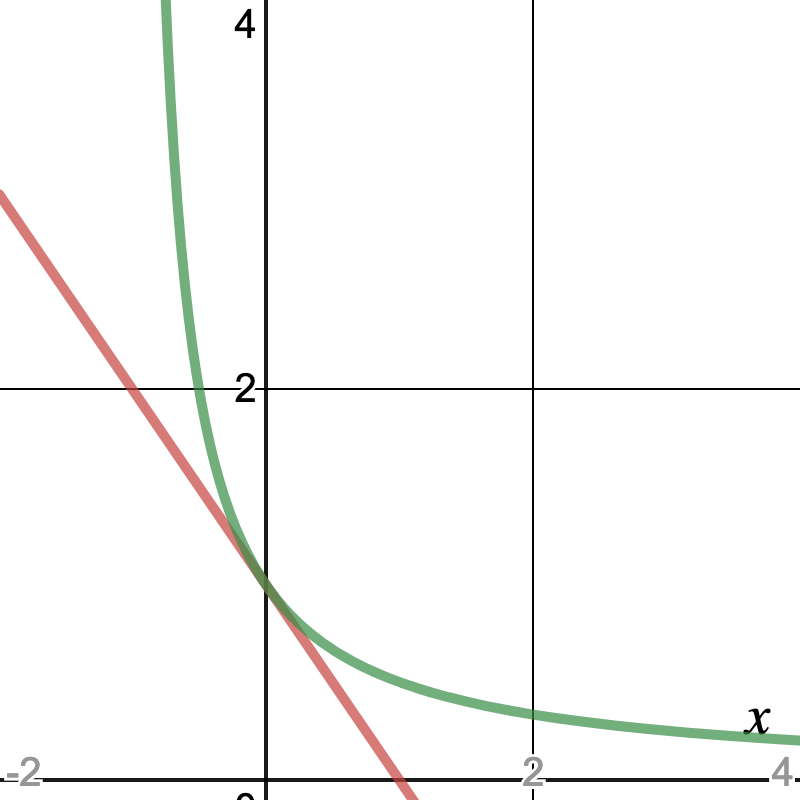
\includegraphics[width=\textwidth]{Figures_Part_3/tangent_line_approx.png}
        \caption{Tangent line approximation to $f(x)=\frac{1}{1+x}$.}
    \end{subfigure}
    ~
    \begin{subfigure}[h]{.3\textwidth}
        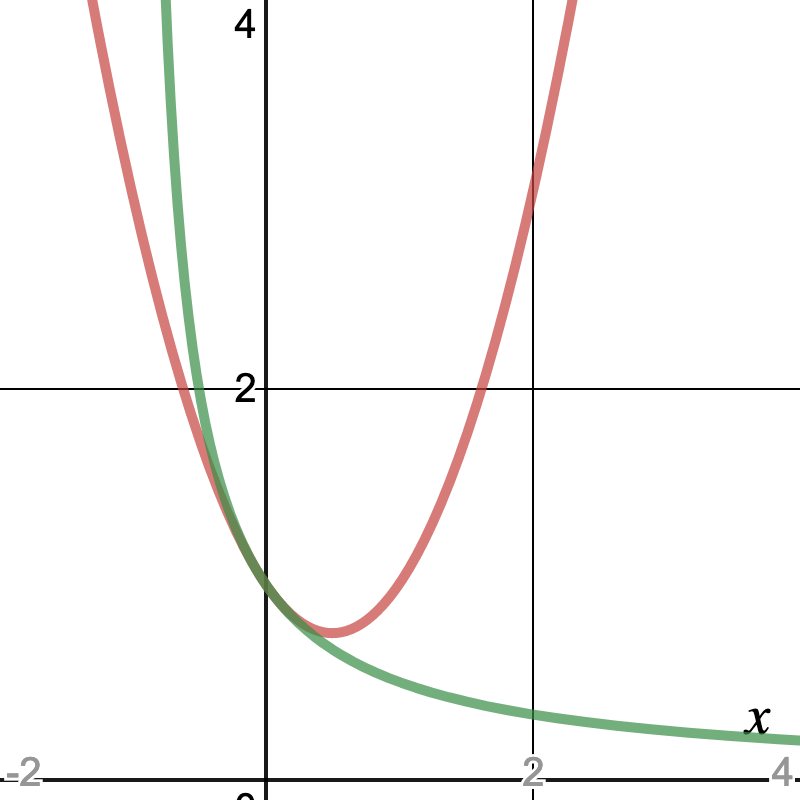
\includegraphics[width=\textwidth]{Figures_Part_3/tangent_quad_approx.png}
        \caption{Tangent quadratic approximation to $f(x)=\frac{1}{1+x}$.}
    \end{subfigure}
    ~
    \begin{subfigure}[h]{.3\textwidth}
        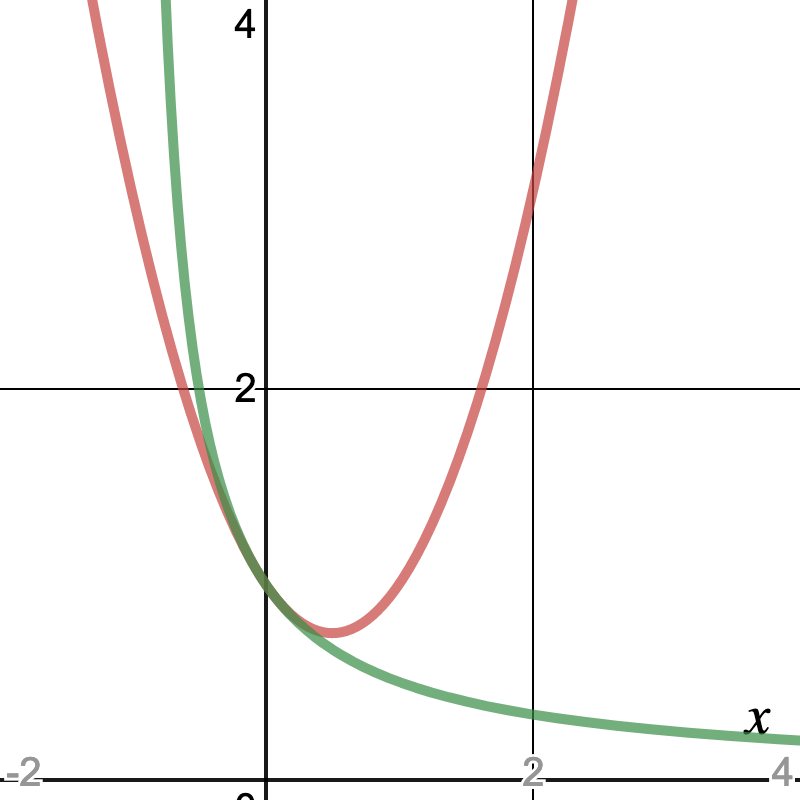
\includegraphics[width=\textwidth]{Figures_Part_3/tangent_quad_approx.png}
        \caption{Tangent cubic approximation to $f(x)=\frac{1}{1+x}$.}
    \end{subfigure}
\end{figure}

Let us think for a moment about how we may construct a series that gives us the above approximations and more.  If we are to pick a point $x=a$ to build our approximation from, then the approximation should have the same value as the function at the point $a$.  So, the zeroth order approximation (i.e., the zeroth term in the series we're building) should be $f(a)$.  Notice that $f(a)$ occurs in the tangent line approximation.  Next, if we take a first order approximation, this should give us an equation for a line. The best approximation around $a$ to the function $f(x)$ with a line would be the tangent line approximation.  The first derivative tells us the information about the slope.  Now, notice the tangent line approximation above contains the zeroth order approximation as well. Functions also tend to have some curvature to them and this is captured nicely by the second derivative of the function at the point $a$.  Now we can add in this second derivative information to get a tangent quadratic
\[
f(a)+f'(a)(x-a)+\frac{f''(a)}{2!}(x-a)^2.
\]
This would be our second order approximation. Similarly, we can build the tangent cubic (or third order approximation) by
\[
f(a)+f'(a)(x-a)+\frac{f''(a)}{2!}(x-a)^2+\frac{f'''(a)}{3!}(x-a)^3.
\]
Taking this pattern in mind, we can create the $N^\textrm{th}$ order approximation to be
\[
f(a)+f'(a)(x-a)+\frac{f''(a)}{2!}+\cdots + \frac{f^{(N)}(a)}{N!}(x-a)^N.
\]
As it turns out, for many functions we can continue this process infinitely and create a power series that exactly matches the function we started with.

\begin{df}{Taylor Series}{taylor_series}
Given a function $f(x)$ that is \emph{analytic} in a region around the point $x=a$, we can construct the \boldgreen{Taylor series centered at $x=a$}
\[
\sum_{n=0}^\infty \frac{f^{(n)}(a)}{n!}(x-a)^n
\]
which is equal to the function $f(x)$ (on a sufficiently small interval $(a-\epsilon, a+\epsilon)$. If we let $a=0$, we call this the \boldgreen{Maclaurin series}.  
\end{df}

Though the definition above only guarantees that the Taylor series is equal to the function on a small interval, many functions we care about will satisfy
\[
f(x)=\sum_{n=0}^\infty \frac{f^{(n)}(a)}{n!}(x-a)^n
\]
for large intervals or even all real numbers.  

\begin{ex}{Maclaurin Series for $e^x$}{maclaurin_exp}
Consider the function $f(x)=e^x$.  We consider constructing the Maclaurin series (Taylor series centered at $x=0$) for $e^x$ by
\[
\sum_{n=0}^\infty \frac{f^{(n)}(0)}{n!}x^n.
\]
Now, note that $f^{(n)}(x)=e^x$ and so $f^{(n)}(0)=1$ for every $n$.  Hence we have that the Maclaurin series for $e^x$ is
\[
\sum_{n=0}^\infty \frac{x^n}{n!}.
\]
It turns out that we have
\[
e^x = \sum_{n=0}^\infty \frac{x^n}{n!}
\]
for all real numbers.
\end{ex}

It's nice to see a few examples of this construction, so let us consider another example.

\begin{ex}{Maclaurin Series for $\ln(1+x)$}{maclaurin_ln}
Consider the function $f(x)=\ln(1+x)$.  We can build the Maclaurin series for $f(x)$ using
\[
\sum_{n=0}^\infty \frac{f^{(n)}(0)}{n!}x^n.
\]
Now we should take a few derivatives of $f(x)$ to see the pattern we need.
\begin{align*}
    f(x)&= \ln(1+x) ~\implies~ f(0)=0\\
    f'(x)&=\frac{1}{1+x} ~\implies~ f'(0)=1=0!\\
    f''(x)&= -\frac{1}{(1+x)^2} ~\implies~ f''(0)=-1=-1!\\
    f'''(x)&= \frac{2}{(1+x)^3} ~\implies~ f'''(0)=2=2!\\
    f^{(4)}(x)&= -\frac{6}{(x+1)^4} ~\implies~ f^{(4)}(0)=-6=-3!.
\end{align*}
So we have that $f^{(n)}(0)=(-1)^{n-1}(n-1)!$ for $n\geq 1$. So our series takes the form
\[
\sum_{n=1}^\infty \frac{(-1)^{n-1}(n-1)!}{n!}x^n = \sum_{n=1}^\infty \frac{(-1)^{n-1}}{n}x^n.
\]
It turns out here that we have 
\[
\ln(1+x)=\sum_{n=1}^\infty \frac{(-1)^{n-1}(n-1)!}{n!}x^n = \sum_{n=1}^\infty \frac{(-1)^{n-1}}{n}x^n
\]
for $x\in (-1,1)$.  
\end{ex}

\begin{exercise}
Determine the radius of convergence of the power series for $\ln(1+x)$.
\end{exercise}

Taylor series granted us the ability to create power series representations of functions.  However, not all functions have a useful Taylor series.  The prototypical example is the \emph{bump} function
\[
f(x) = \begin{cases} e^{-\frac{1}{x^2}} & \textrm{if $\neq 0$}\\ 0 & \textrm{if $x=0$} \end{cases}.
\]
If one computes $f^{(n)}(0)$ they find that it is zero for each $n$. So the Taylor series centered at $0$ is the zero series! Even though the function is infinitely differentiable at $x=0$, it isn't analytic there.

\section{Operations with Power Series}
% ADD IN POWER SERIES SUBSTITUTION like $e^{x^2}$ into the series for $e^x$.
Since we created power series to essentially be polynomials, we hope to gain some of the nice properties of polynomials as well.  Even though the sums are infinite, it turns out that we still get integral and derivative properties like the sum and product rule.  So, given a power series representation for a function (where the $x$ are within the radius of convergence)
\[
f(x)=\sum_{n=0}^\infty a_n x^n,
\]
we want to consider
\[
\frac{d}{dx} f(x) \qquad \textrm{and} \qquad \int f(x) dx.
\]
Since the derivative and integral are \emph{linear operators} (more on this later) we know they satisfy the sum and constant multiple rules which leads us to
\[
\frac{d}{dx} f(x) = \frac{d}{dx} \sum_{n=0}^\infty a_n x^n = \sum_{n=0}^\infty a_n \frac{d}{dx} x^n
\]
and
\[
\int f(x) dx = \int \sum_{n=0}^\infty a_nx^n dx = \sum_{n=0}^\infty a_n \int x^n dx.
\]

Let us concentrate first on differentiating the power series.  So, we have 
\begin{align*}
\frac{d}{dx} \sum_{n=0}^\infty a_nx^n&=\frac{d}{dx} \left(a_0 + a_1x + a_2 x^2 + a_3 x^3 \cdots\right)\\
&= a_1 + 2a_2x+3a_3x^2+\cdots.
\end{align*}
Notice now that the zeroth term in the series has been deleted, and what we have is then
\[
\boxed{\frac{d}{dx} \sum_{n=0}^\infty a_n x^n = \sum_{n=1}^\infty na_n x^{n-1}.}
\]
One could rearrange this series and continue starting it at zero.  We simply have to make sure that the series remains the same after this process.  So, equivalently, one could write
\[
\frac{d}{dx} \sum_{n=0}^\infty a_n x^n = \sum_{n=0}^\infty (n+1)a_{n+1} x^n.
\]

\begin{exercise}
    Verify that the reindexing above makes sense.  
\end{exercise}

\begin{exercise}
    How can we compute second derivatives of a power series? What terms do we lose? What about $n^\textrm{th}$ derivatives?
\end{exercise}

And now we turn to integration. Approaching this in the same way we have
\begin{align*}
    \int \sum_{n=0}^\infty a_n x^n &= \int \left( a_0 +a_1x+a_2x^2+a_3x^3+\cdots\right)dx\\
    &= C+a_0x+\frac{a_1}{2}x^2+\frac{a_2}{3}x^3+\frac{a_3}{4}x^4+\cdots.
\end{align*}
Thus we have that
\[
\boxed{\int \sum_{n=0}^\infty a_n x^n dx = C + \sum_{n=0}^\infty \frac{a_n}{n+1} x^{n+1},}
\]
where $C$ is the undetermined constant from integration.

\begin{exercise}
    Try integrating a power series twice.
\end{exercise}

\begin{ex}{Differentiating and Integrating $e^x$}{diff_int_ex}
We have the power series representation for $e^x$ given by
\[
e^x = \sum_{n=0}^\infty \frac{x^n}{n!}.
\]
Now, if we consider
\begin{align*}
    \frac{d}{dx} \sum_{n=0}^\infty \frac{x^n}{n!} &= \sum_{n=1}^\infty  \frac{nx^{n-1}}{n!}\\
    &=\sum_{n=1}^\infty \frac{x^{n-1}}{(n-1)!}\\
    &= \sum_{n=0}^\infty \frac{x^n}{n!}\\
    &=e^x,
\end{align*}
which is what we expect.  Similarly,
\begin{align*}
    \int \sum_{n=0}^\infty \frac{x^n}{n!} &= C+\sum_{n=0}^\infty \frac{x^{n+1}}{(n+1)n!}\\
    &= C+\sum_{n=0}^\infty \frac{x^{n+1}}{(n+1)!}.
\end{align*}
Now, this should be equal to $e^x+C$ for some undetermined constant $C$. So notice that if we replace $C=D+1$ (which is fine, since $C$ is undetermined), we have
\begin{align*}
    \int \sum_{n=0}^\infty \frac{x^n}{n!} &= D+1+\sum_{n=0}^\infty \frac{x^{n+1}}{(n+1)!}\\
    &= D + 1 + x+\frac{x^2}{2}+\frac{x^3}{3!}+\cdots\\
    &= D+ \sum_{n=0}^\infty \frac{x^n}{n!}\\
    &= D+e^x,
\end{align*}
which does give us what we expect.
\end{ex}

\begin{remark}
With integration and differentiation of series, one just has to be very careful. It often helps to write out part of the series (as shown above) to analyze the problem further.  This is why we begin with examples of functions we already understand well!
\end{remark}

\section{Approximation with Power Series}
A big application of power series is the ability to approximate functions with polynomials.  We did indeed begin developing the Taylor series in order to approximate functions in this way after all.  If we have a function $f(x)$ that is $N$ times differentiable, then we can approximate $f(x)$ around the value $x=a$ as
\[
f(x)\approx \sum_{n=0}^N \frac{f^{(n)}(a)}{n!}(x-a)^n = f(a)+f'(a)(x-a)+\frac{f''(a)}{2!}(x-a)^2+\cdots + \frac{f^{(N)}(a)}{N!}(x-a)^N
\]
which is just a truncation of the Taylor series for $f$. Of course, we may not have that the power series is totally useful (see the end of Section 6.2), but we also have relaxed the assumption that we need to take infinitely many derivatives of $f(x)$.  In fact, it turns out that having two derivatives tends to be plenty as a quadratic approximation works remarkably well.

\begin{df}{Order of an Approximation}{order_of_approx}
Given an approximation of $f(x)$ about the point $x=a$
\[
f(x) \approx \sum_{n=0}^N \frac{f^{(n)}(a)}{n!}(x-a)^n,
\]
we refer to the \boldgreen{order of the approximation} as the highest power of $x$ that appears. In the above case, we would say that this is an $N^\textrm{th}$ order approximation of $f(x)$. 
\end{df}

It's worth seeing some examples of different orders of approximations to see just how well they fare for different functions.  

\begin{ex}{Approximating $e^x$}{approx_ex_order}
Consider the function $e^x$ which has the Taylor series centered at $a=0$ given by
\[
e^x = \sum_{n=0}^\infty \frac{x^n}{n!}.
\]
Then we have the approximations
\begin{align*}
    0^\textrm{th}:~e^x&\approx 1\\
    1^\textrm{st}:~e^x&\approx 1+x\\
    2^\textrm{nd}:~e^x&\approx 1+x+\frac{x^2}{2}.
\end{align*}
\end{ex}

\begin{ex}{How Accurate are Approximations of $\sin(x)$}{approx_sinx}
Consider the function $\sin(x)$ which has the Taylor series centered at $a=0$ 
\[
\sin(x) = \sum_{n=0}^\infty \frac{(-1)^n x^{2n+1}}{(2n+1)!}.
\]
Then we can consider the approximations
\begin{align*}
    0^\textrm{th}:~\sin(x)&\approx 0\\
    1^\textrm{st}:~\sin(x)&\approx x\\
    2^\textrm{nd}:~\sin(x)&\approx x\\
    3^\textrm{rd}:~\sin(x)&\approx x-\frac{x^3}{3!}.
\end{align*}
Due to the fact that $\sin(x)$ is an odd function, we have that the even order approximations don't do any better than the previous odd order approximation.  We can compare the accuracy of the first and third order approximations to the real function values. 
    \begin{table}[H]
        \centering
        \renewcommand{\arraystretch}{1.5}
        \begin{tabular}{c|c|c|c}
            Input & True Value & 3$^\textrm{3rd}$ Order Approx.\\
            \hline
            $x$ & $\sin(x)$ & $x-\frac{x^3}{3!}$\\
            \hline
            0.001 & $\approx 0.000999999$ & $0.0009999998\overline{3}$\\
            \hline
            0.01 &  $\approx 0.00999983$ & $0.0099998\overline{3}$\\
            \hline
            0.1 &  $\approx 0.0998334$ & $0.0998\overline{3}$\\
            \hline
            0.5 & $\approx 0.479426$ & $0.4791\overline{6}$\\
            \hline
            1.0 & $\approx 0.841471$ & $0.8\overline{3}$
        \end{tabular}
        \label{tab:sin_approx}
    \end{table}
    Note that the leftmost column is also the first order approximation. One can see that to six significant digits, the third order approximation does a great job even up to $\sin(1)$.  The upshot is that the third order approximation is far easier to work with than the function $\sin(x)$ itself (which we tend to use the whole series for).
\end{ex}

Since these approximations can do such a great job, it's worthwhile to see how we can use these approximations in practice

\begin{ex}{The Pendulum Problem}{pendulum}
Consider a pendulum system mounted to a frictionless pivot with a bob of mass $m$ a distance $L$ from the pivot. If we pull the bob up by an angle $\theta$, the force if gravity $mg$ is directed downward and thus causes a force of $-mg\sin\theta$ on the bob.  We can draw this system out as follows:
\begin{figure}[H]
    \centering
    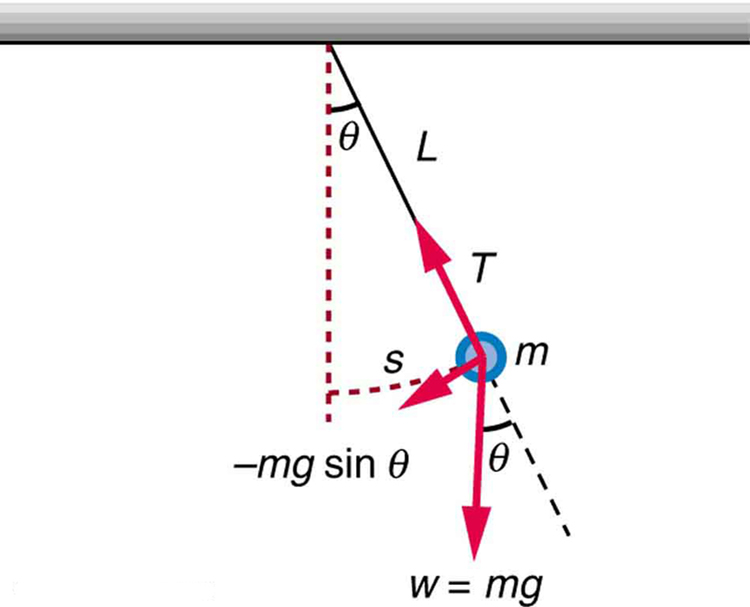
\includegraphics[width=.5\textwidth]{Figures_Part_3/pendulum.jpg}
\end{figure}
Using Newton's second law, we have that the force is equal to the mass times acceleration which leads us to the differential equation
\[
mL\theta'' = -mg\sin \theta. 
\]
This can be well approximated by using the first order approximation for $\sin \theta$. That is, we let
\[
\sin \theta \approx \theta
\]
to arrive at the differential equation
\[
\theta '' = -\frac{g}{L} \theta,
\]
which is the harmonic oscillator equation with $\omega^2 = \frac{g}{L}$. 
\end{ex}

\begin{exercise}
What is the solution to the above approximation of the pendulum equation?
\end{exercise}

\begin{ex}{Classical Diatomic Vibration}{classical_diatomic_vibration}
The Morse potential models the attraction between nuclei in a diatomic molecule.  Specifically, the potential is given by
\[
V(R)=D_e \left[ 1- e^{-a(R-R_e)}\right]^2.
\]
Here, $R$ is the distance between nuclei, $R_e$ is the equilibrium distance, $D_e$ is the dissociation energy of the molecule, and $a$ is a constant.  Stable molecules in low energy states only make small displacements $R-R_e$ from equilibrium and thus we can expand $V(R)$ in a series by
\begin{align*}
V(R) &= D_e\left[ a^2(R-R_e)^2-a^3(R-R_e)^3+\cdots \right]\\
&\approx a^2 D_e(R-R_e)^2.
\end{align*}
Then, Newton's second law with a potential is given by
\[
F= - \frac{dV}{dR}
\]
and so 
\[
F\approx -2a^2 D_e(R-R_e).
\]
Letting $x=(R-R_e)$ and $\omega^2 = \frac{2a^2D_e}{m}$, we have the differential equation
\begin{align*}
    x'' = -\omega^2 x
\end{align*}
which is again the simple harmonic oscillator.
\end{ex}

\begin{exercise}
Verify that the expansion of $V(R)$ about the point $R-R_e$ above is correct.
\end{exercise}

\section{Power Series Solutions to Differential Equations}

Power series provided a tool to approximate functions in order to simplify differential equations, but they also provide a way to solve differential equations as well.  It is in fact very close to the method of undetermined coefficients. The major difference is we (essentially) have to solve for infinitely many coefficients.  We briefly touched on recursive sequences here, and we'll find that these appear here as well. That is to say, if we consider a function given by a power series
\[
f(x) = \sum_{n=0}^\infty a_n x^n
\]
then the $a_n$ coefficients tend to depend on one another.  There are a handful of important functions in physics derived from power series solutions to certain differential equations.  For example, we have Bessel functions, Legendre polynomials, and Laguerre polynomials.  Bessel functions are, for example, found in solving for the wave modes on a circular drum head.  Legendre polynomials are found when solving Laplace's equation in spherical coordinates (we have seen Laplace's equation and will see spherical coordinates in the sequel). Specifically, one sees this when solving for states for the electron in a hydrogen atom.  The Laguerre polynomials also arise in quantum mechanics for the radial states of the Hydrogen atom. Not to mention, if one uses the Morse potential in the Schr\"odinger equation, one will find solutions are forms of Laguerre polynomials.  

To begin, it's easiest to consider some more simple examples of power series solutions.  The two equations we will work with for now are the population growth or decay equation
\[
f'(x)=kf(x)
\]
and the harmonic oscillator equation
\[
f''(x)=-\omega^2 f(x).
\]
As we already know the solutions to this equation, we don't actually need to solve this equations this way.  But, it does provide us a few working examples before we move onto an equation like Legendre's equation. In general, the idea is to take the ansatz that 
\[
f(x) = \sum_{n=0}^\infty a_n x^n
\]
and to take the necessary derivatives of the series and plug it into the given differential equation.  From there, one is able to determine the coefficients $a_n$ which determines the function $f(x)$.  If we are given an initial value (values if the differential equation is higher than first order), then we can explicitly determine every $a_n$ exactly.  Let us see this in action.

\begin{ex}{Power Series Solution for the Population Model}{pop_model_series}
Consider the initial value problem 
\[
f'(x)=kf(x)
\]
with $f(0)=1$.  Then, we know the particular solution to this initial value problem is
\[
f(x)=e^{kx}
\]
which we can find by separation.  So, if power series solutions are to work, we should achieve the same particular solution. We take the ansatz that
\[
f(x) = \sum_{n=0}^\infty a_n x^n
\]
which we can take a derivative of
\[
f'(x) = \sum_{n=1}^\infty na_n x^{n-1}.
\]
Now, we can plug both into our differential equation
\[
\sum_{n=1}^\infty na_n x^{n-1} = k \sum_{n=0}^\infty a_n x^n.
\]
It's usually easier to write out the terms in the series a bit so that we can match them.  So we have
\begin{align*}
    a_1 + 2a_2 x + 3 a_3 x^2 + 4 a_4 x^3 + \cdots &= k(a_0 + a_1 x + a_2 x^2 + a_3 x^3+ \cdots ).
\end{align*}
From this, we can see that we have
\begin{align*}
    a_1 &= k a_0\\
    a_2 &= \frac{k}{2} a_1\\
    a_3 &= \frac{k}{3} a_2 \\
    a_4 &= \frac{k}{4} a_3 \\
    &\cdots \\
    a_n &= \frac{k}{n} a_{n-1}.
\end{align*}
Let us also use our initial condition that $f(0)=1$, which means
\begin{align*}
    1=f(0)&=\sum_{n=0}^\infty a_n 0^n\\
    \implies~1&= a_0.
\end{align*}
Now, we can plug this into our above expressions for the coefficients which gives us
\begin{align*}
    a_1 &= k \\
    a_2 &= \frac{k^2}{2!} \\
    a_3 &= \frac{k^3}{3!}  \\
    a_4 &= \frac{k^4}{4!} \\
    &\vdots \\
    a_n &= \frac{k^n}{n!}.
\end{align*}
This gives us the particular solution
\begin{align*}
f(x) &= \sum_{n=0}^\infty \frac{k^n}{n!} x^n\\
&= \sum_{n=0}^\infty \frac{(kx)^n}{n!}\\
&= e^{kx}.
\end{align*}
Thus we have found exactly what we expected!
\end{ex}

\begin{exercise}
Carefully go through each step above and work out any details you feel are missing.
\end{exercise}

\begin{ex}{Power Series Solution for the Harmonic Oscillator}{power_series_for_harmonic_oscillator}
Consider the differential equation
\[
f''(x) = -\omega^2 f(x).
\]
We wish to find the general solution via a power series solution. We already know the general solution for this equation is of the form
\[
f(x)=C_1 \cos(\omega x)+C_2 \sin(\omega x)
\]
and so we should verify the power series allow us to find the same general solution.  So, we have the power series ansatz
\[
f(x) = \sum_{n=0}^\infty a_n x^n
\]
and thus
\begin{align*}
    f'(x) &= \sum_{n=1}^\infty na_n x^{n-1}\\
    f''(x)&= \sum_{n=2}^\infty n(n-1) x^{n-2}.
\end{align*}
We then plug in $f(x)$ and $f''(x)$ to the differential equation to get
\[
\sum_{n=2}^\infty n(n-1)a_n x^{n-2} = -\omega^2 \sum_{n=0}^\infty a_n x^n.
\]
Once again, I believe it is helpful to write out some of the terms of the series
\begin{align*}
    2a_2 +6a_3 x + 12 a_4 x^2 + 20 a_5 x^3 + \cdots &= \omega^2 (a_0 + a_1 x + a_2 x^2 + a_3 x^3 + \cdots ).
\end{align*}
This gives us the equations
\begin{align*}
a_2 &= \frac{-\omega^2}{2} a_0\\
a_3 &= \frac{-\omega^2}{6} a_1\\
a_4 &= \frac{-\omega^2}{12} a_2\\
a_5 &= \frac{-\omega^2}{20} a_3.
\end{align*}
Then we can determine the even coefficients $a_{2n}$ in terms of $a_0$ and the odd coefficients $a_{2n+1}$ in terms of $a_1$.  So we have
\begin{align*}
    a_2 &= \frac{-\omega^2}{2} a_0 &&& a_3 &= \frac{-\omega^2}{6} a_1\\
    a_4 &= \frac{\omega^4}{24} a_0 &&& a_5 &= \frac{\omega^4}{120} a_1\\
    &\vdots &&& &\vdots\\
    a_{2n} &= \frac{(-1)^n\omega^{2n}}{(2n)!}a_0 &&& a_{2n+1} &= \frac{(-1)^n\omega^{2n}}{(2n+1)!} a_1.
\end{align*}
Hence, the solution to the differential equation can be written as an even power series plus an odd power series as
\begin{align*}
    f(x)&= a_0 \sum_{n=0}^\infty \frac{\omega^{2n}}{(2n)!}x^{2n} + \frac{a_1}{\omega} \sum_{n=0}^\infty \frac{\omega^{2n+1}}{(2n+1)!} x^{2n+1}.
\end{align*}
If we rename $C_1 = a_0$ and $C_2 = \frac{a_1}{\omega}$ then we have
\begin{align*}
    f(x)&=C_1 \sum_{n=0}^\infty \frac{(\omega x)^{2n}}{(2n)!} + C_2 \sum_{n=0}^\infty \frac{(\omega x)^{2n+1}}{(2n+1)^1}\\
    &= C_1 \cos(\omega x)+C_2 \sin(\omega x).
\end{align*}
Again, we found exactly what we needed from the power series ansatz. Notice I made the substitution that $C_2=\frac{a_1}{\omega}$. This made the functions come out to being exactly what we want.  This is fine to do since $a_1$ is undetermined, so $\frac{a_1}{\omega}$ is undetermined as well.
\end{ex}

\begin{exercise}
Again, verify each step in the above solution and fill in any work you need.
\end{exercise}

\section{Orthogonal Polynomials from Power Series Solutions}

Throughout physics and chemistry there are equations that arise again and again.  A prime example would be the simple harmonic oscillator equation.  It would be a reasonable thought to believe that any oscillating system could be approximated by a harmonic oscillator.  There are of course other types of systems that will continue to pop their heads out in new ways.

We have solved some boundary value problems in 1-dimensional space, but when moving to higher dimensions, especially, when dealing with a specific geometry such as a rectangle, circle, disk, cylinder, or sphere for example, new equations begin to appear. It seems that the underlying geometry is very important for these boundary value problems. In fact, different geometrical objects may not even have a boundary! Take for example the unit circle which is the set of all points 
\[
\textrm{Unit Circle} = \left\{ e^{i \theta} ~|~ \theta \in [0,2\pi]\right\}.
\]
There is in fact no boundary for this shape. If you imagine walking along a circle, you'll never find the end of it.

\subsection{Legendre's Equation}

Eventually, we will try to understand the quantum mechanical solution to the hydrogen atom problem.  In the sequel, we build up the ability to do calculus in multiple dimensions and will solve some partial differential equations in higher dimensions.  Blackboxing some notation and terminology for now, the Schr\"odinger equation that describes the electron orbiting a proton (i.e., a hydrogen atom) has the Hamiltonian
\[
H=-\frac{\hbar^2}{2\mu} \nabla^2 - \frac{Ze^2}{4\pi \epsilon_0 r}
\]
where $r$ is the radial coordinate in the spherical coordinate system.  Recall Schr\"odinger's equation is then
\[
H\Psi(r,\theta, \phi) = E\Psi(r, \theta, \phi),
\]
where $r,\theta,\phi$ are the three spherical coordinates. The above equation turns out to be solvable using separation of variables, and the equation for the polar angle $\Theta(\theta)$ turns out to be
\[
\frac{\sin \theta}{\Theta} \frac{d}{d\theta}\left( \sin \theta \frac{d\Theta}{d\theta}\right) +A \sin^2 \theta - B = 0.
\]
If one takes the change of variables $P(\cos \theta)$ with $x=\cos \theta$ then the equation reads
\[
(1-x^2)\frac{d^2P}{dx^2}-2x\frac{dP}{dx}+\left(A-\frac{m^2}{1-x^2}\right)P=0.
\]
This is the \boldgreen{associated Legendre's equation}.  This equation turns out to be a bit more involved than \boldgreen{Legendre's equation} which is given by
\[
(1-x^2)f''(x)-2xf'(x)+m(m+1)f(x)=0.
\]
We will solve Legendre's equation instead.  

\subsubsection{Solving Legendre's Equation}

Legendre's equation arises from boundary value problems. Specifically, we have
\[
(1-x^2)f''(x)-2xf'(x)+m(m+1)f(x)=0,
\]
where we allow $x$ to be in the region $\Omega = [-1,1]$ and force $m$ to be a non-negative integer $m=0,1,2,3,\dots$.  The fact $m$ takes on just those values is that, for example, other requirements in the other variables present in Schr\"odinger's equation place a restriction on $m$. The parameter $m$ being restricted to non-negative integers is once again an example of quantization.  If we relate this differential equation to the true physics, this is saying that we have a discrete amount allowed states in the system.  We've seen this before with the particle in the 1-dimensional box.  We will also require the solutions to this equation for any $m$ to be \emph{normalized}. This is defined below, but in essence it is the requirement that the integral of each of the solution functions (for each $m$) is finite (and in fact equal to one).  This solves the problem uniquely for each $m$.

Much of the above is extra detail that one will eventually spend more time analyzing. For now, we want to solve this equation and we take the ansatz that $f(x)$ can be written as a power series
\[
f(x)=\sum_{n=0}^\infty a_n x^n.
\]
Then we can take the necessary derivatives
\begin{align*}
    f'(x)&=\sum_{n=1}^\infty na_n x^{n-1}\\
    f''(x)&= \sum_{n=2}^\infty n(n-1) a_n x^{n-2}.
\end{align*}
We can plug this into Legendre's equation to get
\begin{align*}
    (1-x^2)f''(x)-2xf'(x)+m(m+1)f(x)&=0\\
    (1-x^2)\sum_{n=2}^\infty n(n-1)a_n x^{n-2} - 2x \sum_{n=1}^\infty na_n x^{n-1} +m(m+1) \sum_{n=0}^\infty a_n x^n &=0\\
    \sum_{n=2}^\infty n(n-1) a_n x^{n-2} - \sum_{n=2}^\infty n(n-1)a_n x^n -\sum_{n=1}^\infty 2n a_n x^{n}+\sum_{n=0}^\infty m(m+1)a_n x^n &=0. 
\end{align*}
It is helpful to reindex the sums here to have all the powers of $x$ be the same so that we can relate each term slightly easier. So we have
\begin{align*}
    \sum_{n=0}^\infty (n+2)(n+1) a_{n+2} x^n - \sum_{n=2} n(n-1) a_n x^n - \sum_{n=1}^\infty 2na_n x^n +\sum_{n=0}^\infty m(m+1)a_n x^n &=0.
\end{align*}
Then if we make all the starting terms agree as well we have
\begin{align*}
    0&= \sum_{n=0}^1 (n+2)(n+1)a_{n+2}x^n -\sum_{n=1}^1 2na_n x^n +\sum_{n=0}^1
    m(m+1)a_n x^n\\
    &\quad + \sum_{n=2}^\infty \left[ (n+2)(n+1)a_{n+2}-n(n-1)a_n -2na_n +m(m+1)an\right]x^n.
\end{align*}
By setting the infinite sum equal to zero, we find $a_{n+2}$ in terms of $a_n$ by
\[
a_{n+2} = -\frac{(m-n)(m+n+1)}{(n+2)(n+1)}a_n.
\]
The finite sums above must also be zero and so
\begin{align*}
    0&= \sum_{n=0}^1 (n+2)(n+1)a_{n+2}x^n -\sum_{n=1}^1 2na_n x^n + \sum_{n=0}^\infty m(m+1)a_n x^n \\
    &= 2a_2 + 6a_3 x - 2a_1 x + m(m+1)a_0 + m(m+1) a_1 x\\
    &= (2a_2 +m(m+1)a_0)+(6a_3+(m(m+1)-2)a_1)x
\end{align*}
and thus we also have the equations
\begin{align*}
    a_2 &= \frac{m(m+1)}{2}a_0 &&& a_3 &= \frac{m(m+1)-2}{6}a_1\\
        &= \frac{m(m+1)}{2!} a_0 &&&  &= \frac{(m-1)(m+2)}{3!}a_1.
\end{align*}
We can thus solve for the even terms and odd terms from $a_0$ and $a_1$ respectively by
\begin{align*}
    a_{2n} &= (-1)^n \frac{m(m-2)\cdots (m-2n+2)(m+1)(m+3)\cdots (m+2n-1)}{(2n)!}a_0 &&& n&\geq 1\\
    a_{2n+1} &= (-1)^n \frac{(m-1)(m-3)\cdots(m-2n+1)(m+2)(m+4)\cdots (m+2n)}{(2n+1)!}a_1 &&& n&\geq 1.
\end{align*}
So for example, the first few even and first few odd terms are
\begin{align*}
    a_2 &= -\frac{m(m+1)}{2!}a_0 &&& a_3 &= -\frac{(m-1)(m+2)}{3!}a_1\\
    a_4 &= -\frac{m(m-2)(m+1)(m+3)}{4!} a_0 &&& a_5 &= \frac{(m-1)(m-3)(m+2)(m+4)}{5!}a_1.
\end{align*}
This splits up our solution into two linearly independent (even and odd) solutions by
\[
y_1(x)=\sum_{n=0}^\infty a_{2n}x^{2n} \qquad \textrm{and} \qquad y_2(x)=\sum_{n=0}^\infty a_{2n+1}x^{2n+1}.
\]

We then have a polynomial for every choice of $m$ we make.  We will denote these polynomials by $f_m(x)$. For example, notice if we take $m=0$, then we have $a_{2k}=0$ for $k\geq 1$ and so we have that $y_1(x)=a_0$. For this case $y_2(x)$ will not converge unless $a_1=0$.  Thus, when $m=0$ we have the polynomial
\[
f_0(x) = a_0. 
\]
If we take $m=1$, then we find that $a_{2k+1}=0$ for $k\geq 1$ and $y_1(x)$ diverges unless $a_0=0$.  Then we have
\[
f_1(x)= a_1 x.
\]
We can continue this process to find, for example,
\[
f_2(x)=a_0(1-3x^2) \qquad \textrm{and} \qquad f_3(x) = a_1\left( x - \frac{5x^3}{3}\right).
\]
There is a polynomial for each $m$, but I have only listed a few here.

\subsubsection{Orthogonality and Normalization}
It turns out that the polynomials created from this process are \boldgreen{orthogonal} since
\[
\int_{-1}^1 f_i(x)f_j(x)dx = 0
\]
when $i\neq j$.  Previously we saw a relationship like this when we studied a particle in the 1-dimensional box.  The idea is the same.  Since we have the undetermined constants $a_0$ and $a_1$ present for each polynomial (where each is also attached to a different value of $m$), we can \boldgreen{normalize} the polynomials above by requiring that
\[
\int_{-1}^1 |f_i(x)|^2 dx = 1.
\]
In doing this process, we find that the normalize polynomials are
\begin{align*}
    f_0(x)&=\sqrt{\frac{1}{2}} &&& f_1(x)&=\sqrt{\frac{3}{2}} x\\
    f_2(x)&= \sqrt{\frac{5}{8}}(1-3x^2) &&& f_3(x)&=\sqrt{\frac{63}{8}}\left( x -\frac{5x^3}{3}\right).
\end{align*}
One could continue generating normalization constants for each polynomial.

We can then say that this set of normalized polynomials is \boldgreen{orthonormal} which means that
\[
\int_{-1}^1 f_i(x)f_j(x)dx = \delta_{ij} = \begin{cases} 1 & \textrm{if $i=j$}\\ 0 & \textrm{if $i\neq j$}\end{cases}.
\]
It turns out to be orthonormal polynomials that are most useful for us.  These polynmomials correspond to states for a quantum system, and thus they should accurately represent a probability. Hence, the normalization.  The fact that the polynomials are also orthogonal is important in quantum mechanics as well, but it is a topic we will revisit in the sequel. In the next part of this text, we discuss linear algebra where we begin to explore the concepts of vectors in more generality.  In that sense, these polynomials are vectors in a vector space.  It's just that the vector space here is infinite dimensional, and is a bit harder to deal with than the finite dimensional case.

\part{Finite Dimensional Linear Algebra}
\chapter{Vectors and Vector Spaces}
% do stuff for systems of differential equations, matrix exponential and stuff

    \section*{Introduction}
        Often times a single number is not adequate for describing a quantity.  Take for example, position and velocity.  In order to describe the position or velocity of a particle, we need to know where in space the particle lies as well as the direction in space the particle travels along with its speed.  This takes three numbers to describe (since we move in a 3-dimensional space). Compare this to temperature.  At any given point in space, we can describe the temperature with a single number. 
        
        The quantity being described above is called a vector.  Formally, a vector is an object that can be scaled and added to other vectors of the same type. This allows one to think of more abstract objects as vectors. For example, we can think of solutions to Schr\"odinger's equation (which are functions) as being vectors in their own type of vector space.
        
        Another way to think of a vector is as a list of numbers. Computer scientists tend to think this way, and we will adopt this point of view for this part of the class.  The vector space for solutions to differential equations behaves slightly differently.  Here, we cover only finite dimensional spaces which is the key difference between the point of view that a vector is a list of numbers versus the view that vectors satisfy some rules of addition and scaling.
        
        The study of vectors, the spaces they reside in, and how they transform falls under the name \boldgreen{linear algebra}. Whether you have been told or not, linear algebra has dictated much of the mathematics you have learned.  This is due to the fact that computations in linear algebra are generally very tractable.  We saw examples of linear differential equations previously.  One then saw approximation of functions via Taylor series.  Fundamentally, linear algebra underlies both of these subjects. Together, one could turn any non-linear differential equation, into a linear one in which we could solve using a power series.
        
        Linear algebra itself has a huge amount of application.  It is widely used in computation and graphics.  One also sees its use in optimization or machine learning.  Quantum mechanics is deeply rooted in linear algebra as well. However, aside from spin systems, quantum systems have an underlying vector space which is infinite dimensional!  For now, we will stick with the finite dimensional case.
        
        \section{Vector Spaces}
        
        Vector spaces are the houses in which vectors can live.  Of course, before we talk about the spaces these objects live in, we should describe the objects as well. The two important quantities in vectors are the vectors themselves and the numbers that scale them.  We'll define these immediately.
        
        \begin{df}{Scalar}{scalar}
        A \boldgreen{scalar} \index{scalar} is an element of a \emph{field} $\mathbb{F}$.  Typically, we take scalars to be numbers $x\in \R$ or $z\in \C$. In other words, we choose our field $\mathbb{F}$ to be equal to $\R$ or $\C$.
        \end{df}
        
        I won't define what a field is here, since we don't need that definition at all.  We will always be working with scalars that are real or complex numbers and we will avoid other scalars.  That isn't to say they aren't important, we just don't need them for our applications.
        
        \begin{exercise}
            If you are interested, look up what a field is and show that $\R$ and $\C$ are fields.
        \end{exercise}
        
        With that in place, we can describe vectors and their associated spaces in a single definition.  
        
        \begin{df}{Vectors and Vector Spaces}{vector}
            A \boldgreen{vector space} $V$ over a field $\mathbb{F}$ is a set of elements we call \boldgreen{vectors} that satisfy the following properties. Take vectors $\vecu,\vecv,\vecw \in V$ and scalars $\alpha, \beta \in \mathbb{F}$. Then, we require that $\alpha\vecv + \beta\vecu \in V$ and 
            \begin{enumerate}[(i)]
                \item (Commutivity of vector addition)
                \[
                \vecu+\vecv=\vecv+\vecu
                \]
                \item (Associativity of vector addition)
                \[
                \vecu+(\vecv+\vecw)=(\vecu+\vecv)+\vecw;
                \]
                \item (Neutral element) There exists $\zerovec$ such that
                \[
                \zerovec+\vecv=\vecv;
                \]
                \item (Inverse element) For each $\vecv$ there exists $-\vecv$ such that
                \[
                \vecv+(-\vecv)=\zerovec;
                \]                
                \item (Assosciativity of scalar multiplication) We have
                \[
                \alpha(\beta \vecv)=(\alpha \beta)\vecv;
                \]
                \item (Distribution over vector addition) we have
                \[
                \alpha(\vecu+\vecv)=\alpha \vecu + \alpha \vecv;
                \]
                \item (Distribution over field addition) we have
                \[
                (\alpha+\beta)\vecv = \alpha \vecv + \beta \vecv;
                \]
                \item (Unit element) There exists $1\in \mathbb{F}$ such that
                \[
                1\vecv = \vecv.
                \]
            \end{enumerate}
        \end{df}
        
        One can try to remember the above rules by the acronym $CANI ADDU$.  The first four have to do with the addition operation and the last four have to do with the scalar multiplication.
        
        \begin{remark}
            It is a common practice to denote vectors as bold symbols or with arrows over the top.  Here we use both to make them more distinguished.  For example, above we used $\vecu$ and $\vecv$ to denote a vector.  We also tend to use Greek letters to denote scalars.  Above we used $\alpha$ and $\beta$ for scalar elements.
        \end{remark}
        
        Now, the above definition is very abstract and we will continually revisit it. But, for now, we should think of vectors as being real geometrical and physical quantities.   In short, a vector space allows for addition of elements we call vectors and scaling of vectors by numbers we calls scalars. 
        
        The geometrical picture of a vector is often most helpful.  Typically, we represent a vector $\vecv$ as an arrow starting with a tail at the origin 0, and head at the desired point. We often do not distinguish a vector $\vecv$ from the point at which the tip lies.  Let us consider the following.
        
        \begin{ex}{Vectors in the Plane $\R^2$}{planar_vectors}
            We denote the 2-dimensional real plane by the symbol $\R^2$. This is a vector space of 2-dimensions with underlying field the real numbers $\R$. The naming convention follows that of the 1-dimensional real line $\R$.  The plane simply has two copies of the real line that provide coordinates for points in the plane.
            
            When specifying a point in the plane, we must provide two coordinates. We saw this previously with complex numbers when we had to provide both a real and imaginary part.  Here in the plane, we tend to think of providing an $x$-value and a $y$-value in a pair $(x,y)$.  
            
            For example, consider the point $(1,2)\in \R^2$.  Then, we can imagine a vector $\vecv$ with tip at $(1,2)$ and tail at the origin $(0,0)$ being given by
            \[
            \vecv = \begin{pmatrix} 1 \\ 2 \end{pmatrix}.
            \]
        \begin{center}
        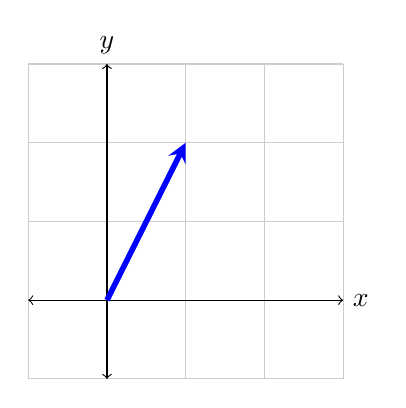
\begin{tikzpicture}
        \draw[thin,gray!40] (-1,-1) grid (3,3);
        \draw[<->] (-1,0)--(3,0) node[right]{$x$};
        \draw[<->] (0,-1)--(0,3) node[above]{$y$};
        \draw[line width=2pt,blue,-stealth](0,0)--(1,2) node[anchor=south west]{$\vecv$};
        \end{tikzpicture}
        \end{center}
        
            Notice that we are barely distinguishing a vector $\vecv$ from the point at which it lies at.  We simply are providing a different notation for it, in some sense.
        \end{ex}
        

        
        \begin{ex}{Positions in 3-Dimensional Space}{position_3dspace}
        The next step up from planar vectors would be vectors in space. Specifically, when we say space we mean a 3-dimensional space $\R^3$.  This is the space we live in in our day to day lives. If you are standing in place, you can measure the position of an object and note that it lies at the point $p=(3,5,4)$ relative to yourself $\zerovec$. This position can described  with a vector and the vector has a bit more structure than just points in space.  This vector begins at your body, and ends at the object. Moreover, it provides you the oriented line segment exiting your eyes and ending at the object. Similarly to the previous example, we would write
        \[
        \vecv = \begin{pmatrix} 3 \\ 5 \\ 4 \end{pmatrix}.
        \]
        We refer to this notation for a vector as a \boldgreen{column vector}. Here, the first entry provides the $x$-coordinate, the second provides the $y$-coordinate, and the third provides the $z$-coordinate. We can picture this vector as follows.
        
        
\begin{center}
\tdplotsetmaincoords{60}{120} 
\begin{tikzpicture} [scale=3, tdplot_main_coords, axis/.style={->,black,thick}, 
vector/.style={-stealth,blue,very thick}, 
vector guide/.style={dashed,red,thick}]

%standard tikz coordinate definition using x, y, z coords
\coordinate (O) at (0,0,0);

%tikz-3dplot coordinate definition using x, y, z coords

\pgfmathsetmacro{\ax}{0.6}
\pgfmathsetmacro{\ay}{1}
\pgfmathsetmacro{\az}{0.8}

\coordinate (P) at (\ax,\ay,\az);

%draw axes
\draw[axis] (0,0,0) -- (1,0,0) node[anchor=north east]{$x$};
\draw[axis] (0,0,0) -- (0,1,0) node[anchor=north west]{$y$};
\draw[axis] (0,0,0) -- (0,0,1) node[anchor=south]{$z$};

%draw a vector from O to P
\draw[vector] (O) -- (P) node[anchor=south east] at (.3,.5,.4){$\vecv$};

%draw guide lines to components
\draw[vector guide]         (O) -- (\ax,\ay,0);
\draw[vector guide] (\ax,\ay,0) -- (P);
\draw[vector guide]         (P) -- (0,0,\az);
\draw[vector guide] (\ax,\ay,0) -- (0,\ay,0);
\draw[vector guide] (\ax,\ay,0) -- (0,\ay,0);
\draw[vector guide] (\ax,\ay,0) -- (\ax,0,0);
\node[tdplot_main_coords,anchor=east]
at (\ax,0,0){};
\node[tdplot_main_coords,anchor=west]
at (0,\ay,0){};
\node[tdplot_main_coords,anchor=south]
at (0,0,\az){};
\node[tdplot_main_coords, anchor=south east] at (0,0,0){$\zerovec$};
\node[tdplot_main_coords, anchor=west] at (\ax,\ay,\az){$p$};
\end{tikzpicture}
\end{center}

        If $p$ moves over time, then our vector $\vecv$ changes over time as well. We'll often denote this $\vecv(t)$.  It's possible the position of an object changes due to interactions with the environment or other objects.  All to come later.
        \end{ex}
        
        Great, we have some objects, but what can we do with them?  As it turns out, we can do quite a bit.  For the most part, anything we could do with numbers, we can do with vectors.  However, we have to be comfortable looking at things in new ways.
        
        \section{Vector Algebra}
        
        Described in the vector space definition is an operation called \boldgreen{vector addition}.  Given two vectors $\vecu$ and $\vecv$, we can create a new vector
        \[
        \vecw = \vecu + \vecv
        \]
        We then required that addition is a commutative operation and so we also have that
        \[
        \vecw = \vecv+\vecu
        \]
        Pictorially, what do we do when we add vectors? We take $\vecu$ and attach the tail of $\vecv$ to the head $\vecu$. 
        
        \begin{center}
        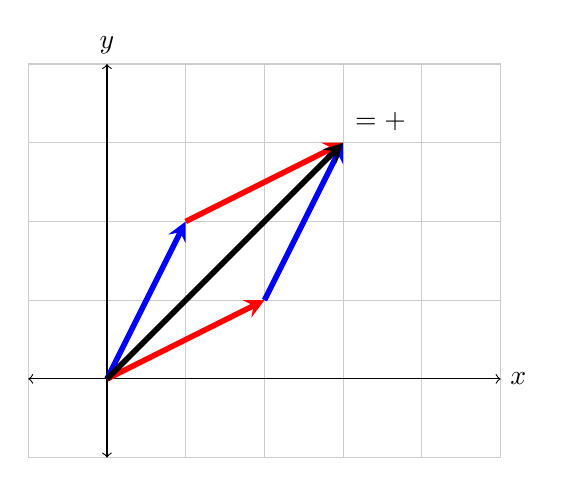
\begin{tikzpicture}
        \draw[thin,gray!40] (-1,-1) grid (5,4);
        \draw[<->] (-1,0)--(5,0) node[right]{$x$};
        \draw[<->] (0,-1)--(0,4) node[above]{$y$};
        \draw[line width=2pt,blue,-stealth](0,0)--(1,2) node[anchor=east] at (.5,1){$\vecu$};
        \draw[line width=2pt, red, -stealth](0,0)--(2,1) node[anchor=north] at (1,.5){$\vecv$};
        \draw[line width=2pt, red, -stealth](1,2)--(3,3) node[anchor=south] at (2,2.5){$\vecv$};
        \draw[line width=2pt, blue, -stealth](2,1)--(3,3) node[anchor=west] at (2.5,2){$\vecu$};
        \draw[line width=2pt, black, -stealth](0,0)--(3,3) node[anchor=south west]{$\vecw=\vecu+\vecv$};
        \end{tikzpicture}
        \end{center}
        
        From this diagram, you can see why the operation is commutative.  Both paths, $\vecu+\vecv$ and $\vecv+\vecu$, lead to the same $\vecw$.
        
        As always, repeated addition gives us a form of multiplication. What will this mean here? 
        
        \begin{exercise}
        Draw a 2-dimensional coordinate system ($x$ and $y$ axes), and draw some vector $\vecv$.  Using vector addition, what does $\vecv+\vecv=2\vecv$ look like? Given this, what do you think $\frac{1}{2}\vecv$ will look like? 
        \end{exercise}
        
        When dealing with a vector, we are allowed to scale the length of the arrow.  As in the definition for a vector space, we call this \boldgreen{scalar multiplication}. Since the vector $2\vecv$ has twice the length of $\vecv$, we would expect $\frac{1}{2} \vecv$ to have half the length of $\vecv$.  All of these vectors point in the same direction though.  We have merely scaled their lengths.
        
        \begin{question}
        What happens if we take $-\vecv$ (i.e., $-1\cdot \vecv$)? \emph{Hint: Consider what happens for numbers on a number line when multiplied by $-1$.} 
        \end{question}
        
        \begin{answer}
        It flips the direction of the vector.
        \end{answer}
        
        We can take a look at all of this. 
        
        \begin{center}
        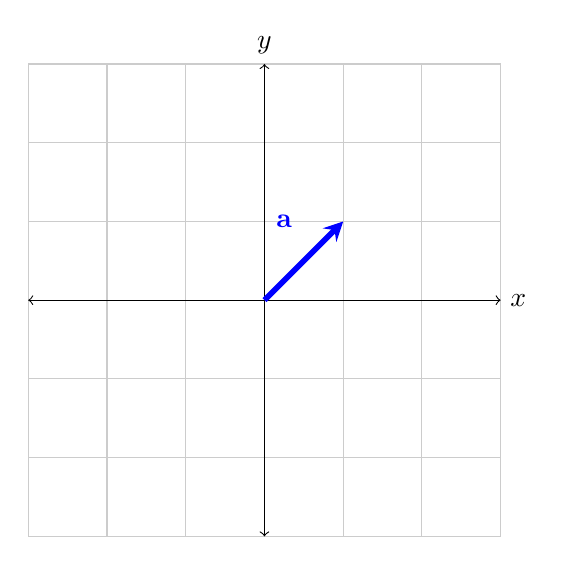
\begin{tikzpicture}
        \draw[thin,gray!40] (-3,-3) grid (3,3);
        \draw[<->] (-3,0)--(3,0) node[right]{$x$};
        \draw[<->] (0,-3)--(0,3) node[above]{$y$};
        \draw[line width=2pt,blue,-stealth](0,0)--(1,1) node[anchor=east] at (.5,1){$\mathbf{a}$};
        \end{tikzpicture}
        \qquad
        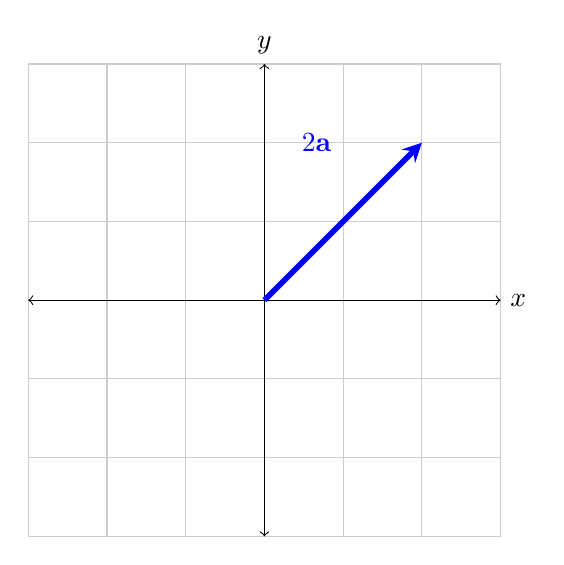
\begin{tikzpicture}
        \draw[thin,gray!40] (-3,-3) grid (3,3);
        \draw[<->] (-3,0)--(3,0) node[right]{$x$};
        \draw[<->] (0,-3)--(0,3) node[above]{$y$};
        \draw[line width=2pt,blue,-stealth](0,0)--(2,2) node[anchor=east] at (1,2){$2\mathbf{a}$};
        \end{tikzpicture}
        
        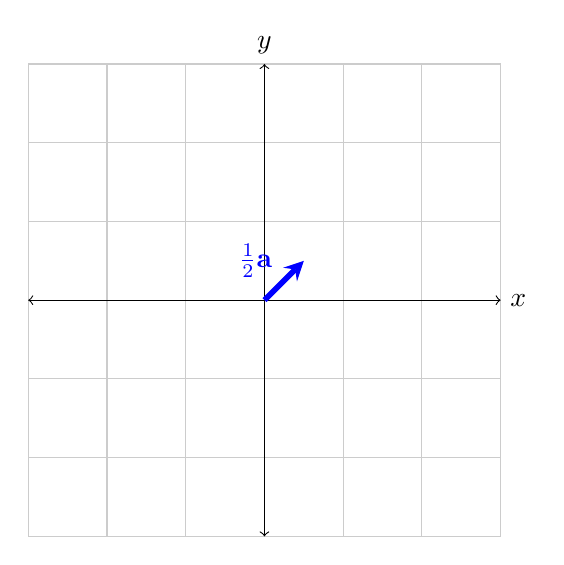
\begin{tikzpicture}
        \draw[thin,gray!40] (-3,-3) grid (3,3);
        \draw[<->] (-3,0)--(3,0) node[right]{$x$};
        \draw[<->] (0,-3)--(0,3) node[above]{$y$};
        \draw[line width=2pt,blue,-stealth](0,0)--(.5,.5) node[anchor=east] at (.25,.5){$\frac{1}{2}\mathbf{a}$};
        \end{tikzpicture}
        \qquad
        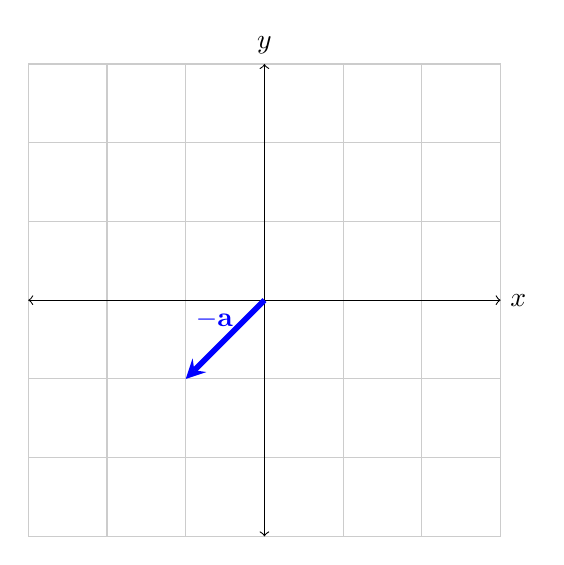
\begin{tikzpicture}
        \draw[thin,gray!40] (-3,-3) grid (3,3);
        \draw[<->] (-3,0)--(3,0) node[right]{$x$};
        \draw[<->] (0,-3)--(0,3) node[above]{$y$};
        \draw[line width=2pt,blue,-stealth](0,0)--(-1,-1) node[anchor=east] at (-.25,-.25){$-\mathbf{a}$};
        \end{tikzpicture}
        \end{center}
        
        In the definition for a vector space, we also required that there exists an inverse element for the vector $\vecv$. That is, we wanted to find a vector $\vecu$ so that $\vecv+\vecu=\zerovec$.  Notice that if we take $\vecu=-\vecv$, then we have $\vecv+(-\vecv)=\zerovec$ using the geometrical notion of vector addition shown above.  Thus, additive inverses of vectors are just vectors of the same length pointing in the opposite direction.  This also gives us a notion of subtracting vectors.
        
        \begin{question}
        Given two arbitrary vectors $\vecu$ and $\vecv$, how can we define $\vecu-\vecv$?  
        \end{question}
        
        \begin{answer}
        As we did above for the inverse case. We write $\vecu+(-\vecv)$ and use the rules for vector addition and scalar multiplication together.
        \end{answer}
        
        \begin{exercise}
        Draw two different vectors $\vecu$ and $\vecv$ and draw the following:
        \begin{itemize}
            \item $\vecu+\vecv$,
            \item $\vecu-\vecv$,
            \item $\vecv-\vecu$.
        \end{itemize}
        \end{exercise}
        
        Now see the picture below.
        
        \begin{center}
        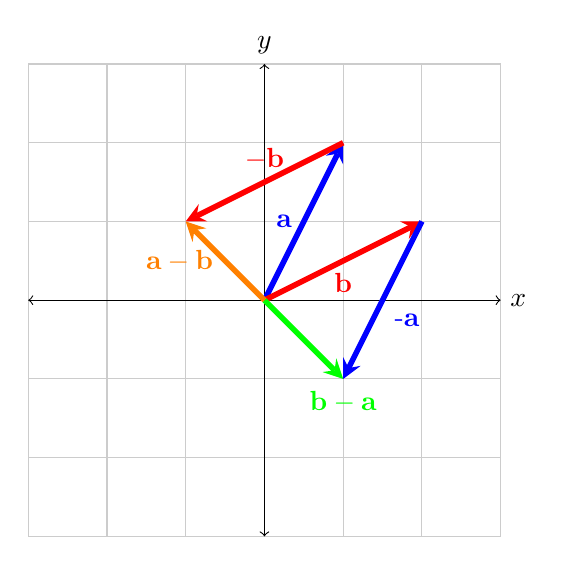
\begin{tikzpicture}
        \draw[thin,gray!40] (-3,-3) grid (3,3);
        \draw[<->] (-3,0)--(3,0) node[right]{$x$};
        \draw[<->] (0,-3)--(0,3) node[above]{$y$};
        \draw[line width=2pt,blue,-stealth](0,0)--(1,2) node[anchor=east] at (.5,1){$\mathbf{a}$};
        \draw[line width=2pt, red, -stealth](0,0)--(2,1) node[anchor=north] at (1,.5){$\mathbf{b}$};
        \draw[line width=2pt, red, -stealth](1,2)--(-1,1) node[anchor=south] at (0,1.5){$-\mathbf{b}$};
        \draw[line width=2pt, blue, -stealth](2,1)--(1,-1) node[anchor=west] at (1.5,-.25){-$\mathbf{a}$};
        \draw[line width=2pt, green, -stealth](0,0)--(1,-1) node[anchor=north]{$\mathbf{b}-\mathbf{a}$};
        \draw[line width=2pt, orange, -stealth](0,0)--(-1,1) node[anchor=east] at (-.5,.5){$\mathbf{a}-\mathbf{b}$};
        \end{tikzpicture}
        \end{center}
        
        \subsection{Linear Combinations}
        
        The most important notion in linear algebra is that of a \boldgreen{linear combination} or \boldgreen{superposition}.  Each and every axiom we required in the definition is put there in order to make sense of linear combinations.  Given two vectors $\vecu,\vecv\in V$ and two scalars $\alpha, \beta \in \mathbb{F}$ from the underlying field $\mathbb{F}$, we call 
        \[
        \alpha \vecu + \beta \vecv
        \]
        a linear combination.  
        
        The requirements in our definition allow us to geometrically interpret scalar multiplication and vector addition as we do, and we can string both of these concepts together in one linear combination.  Vector addition itself is a linear combination where the scalars are chosen to both be one, and scalar multiplication could just be a linear combination with one of the vectors the zero vector.
        
        Linear combinations then allow us to understand how to break up vectors and better use coordinates to describe them.  Similar to coordinates on Earth (i.e., latitude and longitude) we need numbers to describe a vector. But, we also need to know what these numbers are specifying.  We know what latitude and longitude describe on Earth, but these are not the only choice in coordinates we could use!
        
        \section{Vector Components}
        The previous work has still been fairly abstract and has left us without a way to explicitly compute quantities! To work with vectors more effectively, it's necessary to break them down into \boldgreen{components}. We can think of components as coming from coordinates on the vector space. Let us consider the following.
        
        \begin{ex}{Components of a Vector}{vector_components}
        Let us fix an arbitrary vector $\vecv$ in $\R^2$ (i.e., the $xy$-plane).  
        \begin{center}
        \begin{tikzpicture}[vector guide/.style={dashed,red,thick}]
        \draw[<->] (-1,0)--(5,0) node[right]{$x$};
        \draw[<->] (0,-1)--(0,5) node[above]{$y$};
        \draw[line width=2pt,blue,-stealth](0,0)--(4,4) node[anchor=east] at (2,2.5){$\vecv$};
        \draw[vector guide] (4,0) -- (4,4);
        \draw[vector guide] (0,0) -- (4,0);
        \node[anchor=north] at (2,0){$v_x$};
        \node[anchor=west] at (4,2){$v_y$};
        \end{tikzpicture}
        \end{center}
        We can break down this vector into the portions that are in the $x$-direction and $y$-direction.  We say that the component of the vector in the $x$-direction is $v_x$ and the component of the vector in the $y$-direction is $v_y$.  Using the Pythagorean theorem, it follows that the length of the vector is $\|\vecv\|=\sqrt{v_x^2+v_y^2}$. This is exactly how we defined the modulus of a complex number $\|z\|$.
        
        Hence, we would write
        \[
        \vecv=\begin{pmatrix} v_x \\ v_y \end{pmatrix}.
        \]
        \end{ex} 
        
        In the previous two examples we represented vectors by ordered lists of numbers.  This notation is more than adequate, but we do often see vectors presented a different way. When we think of vectors, we tend to think of coordinates presented in the ordered list.  However, we will sometimes wish to change coordinates and so we must consider the other form of notation. These coordinates would then give us different components for a vector.  We will eventually see this.
        
        \section{Vector Algebra with Components}
        Let us work with vectors in space $\R^3$.  These vectors each have three components, so it suffices to specify $\vecv$ as 
        \[
        \vecv = \begin{pmatrix} v_x \\ v_y \\ v_z \end{pmatrix}.
        \]
        One can then also specify the length $\|\vecv\|$ of $\vecv$ by writing
        \[
        \|\vecv\| = \sqrt{ v_x^2 + v_y^2 + v_z^2},
        \]
        which is much like the Pythagorean theorem. If a vector $\unitvec$ has length one, that is, if $\|\unitvec\|=1$, then we say that $\unitvec$ is a \boldgreen{unit vector}. One may also say that $\unitvec$ is a \boldgreen{normalized} vector. We also tend to place hats on unit vectors as opposed to arrows to denote the unit length.
        
        When we write these coordinates for a vector, we are really saying that $\vecv$ points an amount $v_x$ in the $x$-direction, $v_y$ in the $y$-direction, and $v_z$ in the $z$-direction.  So, if we consider unit vectors that point in these different directions, then we can  write $\vecv$ as a linear combination of these vectors.  So, we set
        \[
        \xhat = \begin{pmatrix} 1 \\ 0 \\ 0 \end{pmatrix} \qquad \yhat = \begin{pmatrix} 0 \\ 1 \\ 0 \end{pmatrix} \qquad \zhat = \begin{pmatrix} 0 \\ 0 \\ 1 \end{pmatrix}.
        \]
        We call the above vectors the \boldgreen{unit basis vectors} since they are of  length one and we can write any vector in $\R^3$ as a linear combination of the three of them.  That is, we can write 
        \[
        \vecv = v_x \xhat + v_y \yhat + v_z \zhat.
        \]
        

        Now, we want to be able to understand vector algebra in these components. Let 
        \[
        \vecu = u_x \xhat + u_y \yhat + u_z \zhat \qquad \textrm{and} \qquad \vecv = v_x \xhat + v_y \yhat + v_z \zhat,
        \]
        then we can note the following:
        
        \begin{itemize}
            \item \textbf{Equality:} Vectors are equal when their components are equal,
            \[
            \vecu=\vecv ~~ \textrm{if} ~~ u_x=v_x, ~~ u_y=v_y ~~ \textrm{and} ~~ u_z=v_z.
            \]
            \item \textbf{Addition:} The sum $\vecu + \vecv$ is done by adding components together,
            \[
            \vecu+\vecv=(u_x+v_x)\xhat + (u_y + v_y)\yhat + (u_z + v_z)\zhat.
            \]
            \item \textbf{Scalar Multiplication:} The product $\alpha \vecv$ is obtained by multiplying each component of $\vecv$ by $\alpha$,
            \[
            \alpha \vecv = (\alpha v_x) \xhat + (\alpha v_y)\yhat + (\alpha v_z)\zhat.
            \]
        \end{itemize}
        
        \begin{ex}{Vector Algebra in Space}{vect_alg_space}
            Consider the vectors
            \[
            \vecu = \xhat + \yhat + \zhat = \begin{pmatrix} 1 \\ 1 \\ 1\end{pmatrix} \qquad \vecv = 2\xhat + \yhat = \begin{pmatrix} 2 \\ 1 \\ 0 \end{pmatrix} \qquad \vecw = \xhat + \zhat = \begin{pmatrix} 1 \\ 0 \\ 1 \end{pmatrix}.
            \]
            Then we can compute 
            \[
            \vecu+\vecv = (\xhat+\yhat+\zhat)+(2\xhat + \yhat) = 3\xhat + 2\yhat + \zhat.
            \]
            Or, we can add the column vectors
            \[
            \vecu+\vecv = \begin{pmatrix} 1 \\ 1 \\ 1 \end{pmatrix} + \begin{pmatrix} 2 \\ 1 \\ 0 \end{pmatrix} = \begin{pmatrix} 3 \\ 2 \\ 1 \end{pmatrix}.
            \]
            Of course, we could also sum all three vectors and find
            \[
            \vecu+\vecv+\vecw = 4\xhat + 2\yhat + 2 \zhat = \begin{pmatrix} 4 \\ 2 \\ 2 \end{pmatrix}.
            \]
            We can also scale the vectors. Take for example
            \[
            5 \vecu = 5\xhat + 5\yhat + 5\zhat = \begin{pmatrix} 5 \\ 5 \\ 5 \end{pmatrix}
            \]
            or
            \[
            - \vecv = -2\xhat -\yhat = \begin{pmatrix} -2 \\ -1 \\ 0 \end{pmatrix}.
            \]
            Then, we could consider a linear combination of the vectors like
            \begin{align*}
                5\vecu - \vecv + 2\vecw &= (5\xhat + 5\yhat + 5\zhat) + (-2\xhat -\yhat) + (2\xhat +2\zhat)\\
                &= 5\xhat + 4\yhat +7\zhat\\
                &= \begin{pmatrix} 5 \\ 4 \\ 7 \end{pmatrix}.
            \end{align*}
        \end{ex}
        
        \begin{exercise}
            Draw the picture for the subtraction $\vecu-\vecv$.
        \end{exercise}
        
        \begin{exercise}
        Given $\vecu=(2,3,1)$, $\vecv=(1,-2,0)$, and $\vecw=(5,2,-1)$, find 
        \begin{enumerate}[(a)]
            \item $\boldsymbol{\vec{d}}=2\vecu+3\vecv-\vecw$,
            \item $\|\boldsymbol{\vec{d}}\|$ (the length of $\boldsymbol{\vec{d}}$),
            \item Let $\alpha$ be a scalar.  Does it make sense to consider $\boldsymbol{\vec{r}}=\vecu+\alpha$? Why or why not?
        \end{enumerate}
        \end{exercise}
        
        Given a vector space $V$, we want to find a list of vectors that, by taking a linear combination of said vectors, can form any vector in the vector space $V$.  We call this set of vectors a \boldgreen{basis}. Given a set of vectors $\{\vecv_1,\vecv_2,\dots,\vecv_n\}$, we say that the \boldgreen{span} of the vectors is the set of all vectors that can be written as linear combinations of the vectors in the set.  Specifically, we are looking for all vectors $\vecu$ so that
        \[
        \vecu = \alpha_1 \vecv_1 + \alpha_2 \vecv_2 +\cdots + \alpha_n \vecv_n.
        \]
        Then we can define the span (which is a set) to be
        \[
        \Span(\{\vecv_1,\vecv_2,\dots,\vecv_n\}) = \{\alpha_1 \vecv_1 + \alpha_2 \vecv_2 +\cdots + \alpha_n \vecv_n ~|~ \alpha_i \in \mathbb{F}\}.
        \]
        
        Take for example vectors in the real plane $\R^2$.  We have that the unit basis vectors $\xhat$ and $\yhat$ form a basis for $\R^2$ since any vector $\vecv$ can be written as a linear combination as 
        \[
        \vecv = v_x \xhat + v_y\yhat.
        \]
        Similarly, a vector $\vecu$ in space $\R^3$ can be written as a linear combination of the unit basis vectors $\xhat$, $\yhat$, and $\zhat$ as
        \[
        \vecu = u_x \xhat + u_y \yhat + u_z \zhat.
        \]
        Hence the unit basis vectors for $\R^3$ are also a basis.  One shouldn't have been surprised based on the name we chose!
        
        We can visualize these basis vectors in the plane and make sense of the combinations above. Let us take the vector $\vecv = 2\xhat + 3\yhat$, then we have:
        \begin{center}
        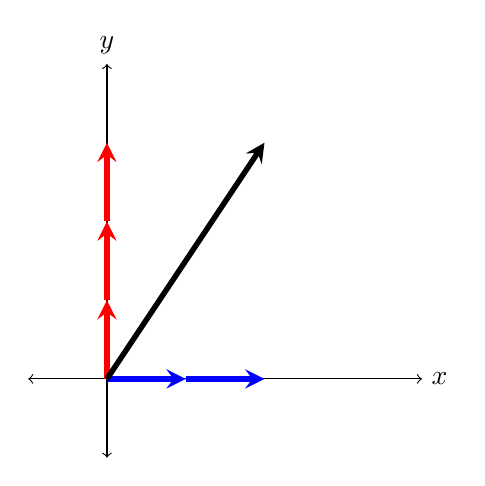
\begin{tikzpicture}[vector guide/.style={dashed,red,thick}]
        \draw[<->] (-1,0)--(4,0) node[right]{$x$};
        \draw[<->] (0,-1)--(0,4) node[above]{$y$};
        \draw[line width=2pt,blue,-stealth](0,0)--(1,0) node[anchor=north] at (1,0){$\xhat$};
        \draw[line width=2pt,blue,-stealth](1,0)--(2,0) node[anchor=north] at (2,0){$\xhat$};
        \draw[line width=2pt, red,-stealth](0,0)--(0,1) node[anchor=east] at (0,1){$\yhat$};
        \draw[line width=2pt, red,-stealth](0,1)--(0,2) node[anchor=east] at (0,2){$\yhat$};
        \draw[line width=2pt, red,-stealth](0,2)--(0,3) node[anchor=east] at (0,3){$\yhat$};
        \draw[line width=2pt,black,-stealth](0,0)--(2,3) node[anchor=north] at (2,3){$\vecv$};
        \end{tikzpicture}
        \end{center}
        
        \begin{ex}{Another Basis for $\R^3$}{another_basis}
        Consider again the vectors
            \[
            \vecu = \xhat + \yhat + \zhat = \begin{pmatrix} 1 \\ 1 \\ 1\end{pmatrix} \qquad \vecv = 2\xhat + \yhat = \begin{pmatrix} 2 \\ 1 \\ 0 \end{pmatrix} \qquad \vecw = \xhat + \zhat = \begin{pmatrix} 1 \\ 0 \\ 1 \end{pmatrix},
            \]
            then these vectors form a basis for $\R^3$. 
            \begin{question}
            How do we show that this is a basis?
            \end{question}
            \begin{answer}
            We must show that any vector $\vecr \in \R^3$ can be written as a linear combination of the three given vectors.
            \end{answer}
            So, let $\vecr = r_x\xhat + r_y\yhat + r_z \zhat$, and we have
            \begin{align*}
                \vecr &= \alpha_1 \vecu + \alpha_2 \vecv + \alpha_3 \vecw\\
                u_x \xhat + u_y \yhat + u_z \zhat &= \alpha_1 (\xhat + \yhat + \zhat) + \alpha_2 (2\xhat + \yhat) + \alpha_3 (\xhat + \zhat)\\
                u_x \xhat + u_y \yhat + u_z \zhat &= (\alpha_1 +2\alpha_2 + \alpha_3)\xhat + (\alpha_1 +\alpha_2)\yhat + (\alpha_1 +\alpha_3)\zhat.
            \end{align*}
            This gives us three equations. One for each component of the vector $\vecu$. Specifically, we have
            \begin{align*}
                u_x &= \alpha_1 + 2\alpha_2 + \alpha_3 \\
                u_y &= \alpha_1 + \alpha_2\\
                u_z &= \alpha_1 + \alpha_3.
            \end{align*}
            The goal is now to determine whether or not this system of equations can be solved in general!
        \end{ex}
        
        Now that we have some structure, it's worth seeing one example of an application for vectors. There are plenty more reasons, but with the tools we already have, this example is not too hard to work with. Plus, it is rather fundamental.
        
        \begin{ex}{Center of Mass}{center_of_mass}
        If we have $n$ point masses each with a mass $m_i$ and position $\boldsymbol{\vec{r}}_i$, then the center of mass can be written
        \[
        \boldsymbol{\vec{R}}_{cm}=\frac{1}{M}(m_1\boldsymbol{\vec{r}}_1+m_2 \boldsymbol{\vec{r}}_2 + \cdots + m_n \boldsymbol{\vec{r}}_n)=\frac{1}{M}\sum_{i=1}^n m_i \boldsymbol{\vec{r}}_i
        \]
        where
        \[
        M=\sum_{i=1}^n m_i
        \]
        is the total mass.
        
        The way to think about this is as averaging the position of these particles but keeping track of how much each weighs.  For example, imagine two masses $m_1$ and $m_2$ in one dimension.  If $\boldsymbol{\vec{r}}_1=1$ and $\boldsymbol{\vec{r}}_2=-1$, then if $m_2>m_1$, the center of mass should be closer to $m_2$ and thus negative.
        \end{ex}
        

        
        The most important vector space for us will be $\R^n$ where $n$ is a positive integer.  $\R^2$ is familiar to us, as it is usually called the $xy$-plane. $\R^3$ is as well, as we usually think of the space surrounding us as being 3-dimensional.
        
        \begin{remark}
        For us, we will always assume that the tail of vectors starts at $\zerovec$ (the origin) unless otherwise stated.  When we get to vector fields, this will be a bit different.
        \end{remark}
        
        \begin{ex}{Examples of Vectors}{examples_of_vecs}
        When the field of scalars are real numbers, we have some example vector spaces. Note, for these, all the scalars $v_x,v_y,v_z,$ or $v_i$ are all real numbers.
        \begin{itemize}
            \item A vector $\vecv \in \R^1=\R$ is just a real number.
            \item A vector $\vecv \in \R^2$ is written as 
            \[
            \vecv = v_x \xhat + v_y \yhat = \begin{pmatrix} v_x \\ v_y \end{pmatrix}.
            \]
            \item A vector $\vecv \in \R^3$ is written as 
            \[
            \vecv = v_x \xhat + v_y \yhat + v_z \zhat = \begin{pmatrix} v_x \\ v_y \\ v_z \end{pmatrix}.
            \]
            \item In general, a vector $\vecv \in \R^n$ is written as
            \[
            \vecv = v_1 \basvec_1 + v_2 \basvec_2 + \cdots + v_n \basvec_n = \begin{pmatrix} v_1 \\ v_2 \\ \vdots \\ v_n \end{pmatrix}.
            \]
            where $\basvec_i$ is the $i$th standard unit basis vector for $\R^n$.
        \end{itemize}
        It is possible that the field of scalars is also the complex numbers, in which case we have analogous vector spaces. Here, we tend to not have special notation for two or three dimensional space and we just put
        \begin{itemize}
            \item A vector $\vecu \in \C^n$ is written as
            \[
            \vecu = u_1 \basvec_1 + u_2 \basvec_2 + \cdots + u_n \basvec_n,
            \]
            where all the $u_i$ are complex numbers.
        \end{itemize}
        \end{ex}
        
        \section{Products of Vectors}
        
        Given two vectors, one would like to make products between them in order to find out how related the two vectors are.  Also, we should be able to decompose any vectors in a vector space into more fundamental components we understand.  We've done this above, but now we would like a way to do this in more generality.
        
        \subsection{The Dot Product}
        \begin{question}
        Given two vectors $\vecu$ and $\vecv$ based at the same point, can we determine the angle $\theta$ between them? 
        \end{question}
        
        \begin{center}
\begin{tikzpicture}
  \draw
    (3,-1) coordinate (a) node[right] {$\vecv$}
    -- (0,0) coordinate (b) node[left] {}
    -- (2,2) coordinate (c) node[above right] {$\vecu$}
    pic["$\theta$", draw=orange, <->, angle eccentricity=1.2, angle radius=1cm]
    {angle=a--b--c};
\end{tikzpicture}
        \end{center}
        
        \begin{answer}
        Yes.  In fact, the way we find this gives us a lot more than just an angle.  It will be a fundamental concept that we will use often.
        \end{answer}
        
        Let's consider the following related question first.  If we have a vector $\vecv$ and a unit vector $\unitvec$, how much of the vector $\vecv$ lies across the vector $\unitvec$? We will denote this quantity by $\vecv\cdot \unitvec$.) The physical way to think about this is to imagine that we are shining a light perpendicularly to $\unitvec$ and we measure the length of the shadow that $\vecv$ would leave on $\unitvec$? Take for example the following illustration.
        
        \begin{center}
        \begin{tikzpicture}[vector guide/.style={dashed,red,thick}]
        \draw[<->] (-1,0)--(4,0) node[right]{$x$};
        \draw[<->] (0,-1)--(0,4) node[above]{$y$};
        \draw[line width=2pt,black,-stealth](0,0)--(2,3) node[anchor=west] at (2,3){$\vecv$};
        \draw[line width=2pt,blue,-stealth](0,0)--(1,0) node[anchor=south west] at (1,0){$\unitvec$};
        \draw[vector guide] (0,-.25) -- (2,-.25) node[anchor=north] at (1,-.25){$\vecv \cdot \unitvec$};
        \end{tikzpicture}
        \end{center}
        
        \noindent Above, one should note that this operation of $\vecv\cdot \unitvec$ is not giving us a new vector, rather it is just providing the length of this shadow being cast.
        
        When the angle is $\theta=0$, then we expect this quantity $\vecv \cdot \unitvec$ to be maximized as the shadow cast by projecting $\vecv$ onto $\unitvec$ will be as long as $\vecv$ is itself. When $\theta=\frac{\pi}{2}$, the quantity will be zero as there will be no shadow cast at all. When $\theta=\pi$, then our quantity would be reversed as to tell us that we would be measuring a shadow pointing the opposite direction of $\unitvec$. This is then the negative of the result that we arrived at when $\theta=0$.  Continuing, if $\theta=\frac{3\pi}{2}$, we would get 0 and lastly if $\theta=2\pi$ this is no different than $\theta=0$.  
        
        What we arrive at with a bit more work is that
        \[
        \vecv\cdot \unitvec=\|\vecv\| \cos \theta.
        \]
        We call this the \boldgreen{dot product} or \boldgreen{inner product} of the vectors $\vecv$ and $\unitvec$. However, we are not required to form this product between a vector and a unit vector. The only difference we see is that the length of the vector we are casting a shadow onto also plays a role in the output of the dot product. Specifically, we have for vectors $\vecv$ and $\vecu$ that the inner product is given by
        \[
        \boxed{\vecu \cdot \vecv = \|\vecu\|\|\vecv\| \cos \theta,}
        \]
        where $\theta$ is again the angle between the two vectors
        
        It turns out that the inner product can be computed in another way.  This fact makes the inner product an indispensable tool. For two vectors given by coordinates $\vecu=(u_x,u_y,u_z)$ and $\vecv=(v_x,v_y,v_z)$ that
        \[
        \boxed{\vecu \cdot \vecv= u_xv_x + u_y v_y + u_z v_z}.
        \]
        Both definitions imply that we have commutivity for this product of vectors. That is,
        \[
        \vecu\cdot \vecv = \vecv \cdot \vecu.
        \]
        They also imply that if we take three vectors, we have
        \[
        (\vecu+\vecv)\cdot \vecw = \vecu \cdot \vecw + \vecv \cdot \vecw.
        \]
        
        \begin{remark}
        If we had vectors $\vecu$ and $\vecv$ that were both elements of $\R^n$, we would compute the dot product just as above. That is, if 
        \[
        \vecu = u_1 \basvec + u_2 \basvec_2 + \cdots + u_n \basvec_n \qquad \vecv = v_1 \basvec_1 + v_2 \basvec_2 + \cdots + v_n \basvec_n,
        \]
        then we have
        \[
        \vecu \cdot \vecv = u_1 v_1 + u_2 v_2 +\cdots + u_n v_n = \sum_{i=1}^n u_i v_i.
        \]
        \end{remark}
        
        The inner product gives us special relationships to vectors. It also gives us a natural notion of direction and lets us compare these directions to one another.  Specifically, the inner product lets us see when two vectors point in two perpendicular directions. 
        
        \begin{df}{Orthogonal}{orthogonal}
        Two vectors $\vecu$ and $\vecv$ are \boldgreen{orthogonal} \index{orthogonal} if
        \[
        \vecu\cdot \vecv=0.
        \]
        Orthogonal and perpendicular are synonymous.
        \end{df}
        
        \begin{ex}{Unit Basis Vectors}{unit_basis_vectors}
            Consider the unit basis vectors in $\R^3$,
            \[
            \xhat = \begin{pmatrix} 1 \\ 0 \\ 0 \end{pmatrix}, \qquad \yhat = \begin{pmatrix} 0 \\ 1 \\ 0 \end{pmatrix}, \qquad \zhat = \begin{pmatrix} 0 \\ 0 \\ 1 \end{pmatrix}.
            \]
            Then each of these unit basis vectors are mutually orthogonal to one another.  Specifically, if we take
            \begin{align*}
            \xhat \cdot \yhat &= 1\cdot 0 + 0 \cdot 1 + 0 \cdot 0 = 0\\
            \xhat \cdot \zhat &= 1\cdot 0 + 0 \cdot 0 + 0 \cdot 1 = 0\\
            \yhat \cdot \zhat &= 0 \cdot 0 + 1\cdot 0 + 0 \cdot 1 = 0.
            \end{align*}
        \end{ex}
        
        \begin{exercise}
        Take two vectors $\vecu=2\xhat + \yhat$ and $\vecv=\xhat + \yhat$.  Compute the dot product in both ways.  That is
        \[
        \vecu\cdot \vecv=u_xv_x + u_y v_y=\|\vecu\|\|\vecv\|\cos \theta.
        \]
        Verify that they give the same answer.
        \end{exercise}
        
        \begin{ex}{Work by Constant Force}{work_constant_force}
        The \boldgreen{work} $W$ done by a constant force $\boldsymbol{\vec{F}}$ on a mass $m$ displaced from position $\vecu=u_x \xhat + u_y \yhat + u_z\zhat $ to $\vecv = v_x \xhat + v_y \yhat + v_z \zhat$ is given by
        \[
        W=\forcevec\cdot \displacement
        \]
        where
        \[
        \displacement=\vecv-\vecu.
        \]
        \end{ex}
        
        \subsubsection{Length of a Vector from the Inner Product}
        The inner product of vectors gives us a natural way to compute the length of a vector.  By the way we defined it, we have that the inner product describes the length of a vector lying along another vector.  So, if we allow both vectors input into the inner product to the same vector, we will find this relates to the length. Take a vector $\vecv \in \R^2$, then we can compute
        \[
        \vecv \cdot \vecv = \|\vecv\|\|\vecv\| \cos \theta,
        \]
        but the angle between the vectors is zero and hence
        \[
        \boxed{\vecv\cdot \vecv = \|\vecv\|^2}.
        \]
        Using the other means of computing the dot product, we have
        \[
        \boxed{\vecv \cdot \vecv = \|\vecv\|^2 = v_x^2 + v_y^2}
        \]
        which is just the Pythagorean theorem!  This of course generalizes to 3-dimensions and higher.
        
        The dot product has lead us to one last important definition that we should carry with us throughout the rest of this text and the sequel.  
        
        \begin{df}{Orthonormal}{orthonormal}
            Given a set of vectors $\{\basvec_1,\basvec_2,\dots,\basvec_n\}$ in $\R^n$ we say that this set of vectors is \boldgreen{orthonormal} if each vector $\basvec_i$ is a unit vector and if each pair of vectors $\basvec_i$ and $\basvec_j$ are mutually orthogonal. That is, we have
            \[
            \|\unitvec_i\|=1 \qquad \textrm{for every $i$}
            \]
            and
            \[
            \basvec_i \cdot \basvec_j = 0 \qquad \textrm{if $i\neq j$}.
            \]
            This can all be succinctly written as
            \[
            \basvec_i \cdot \basvec_j = \delta_{ij} = \begin{cases} 1 & \textrm{if $i=j$}\\ 0 & \textrm{if $i\neq j$}\end{cases}.
            \]
            We call $\delta_{ij}$ the \boldgreen{Kronecker delta symbol}.
        \end{df}
        
        \subsubsection{Components via the Inner Product}
            One may also wish to recover components of a vector via the dot product.  For example, if one wants to recover the $x$-component of a vector $\vecv \in \R^3$, then one can compute
            \[
            \vecv \cdot \xhat = v_x \cdot 1 + v_y \cdot 0 + v_z \cdot 0 = v_x.
            \]
            Then we can do this for each component as well by
            \begin{align*}
                \vecv \cdot \yhat &= v_x \cdot 0 + v_y \cdot 1 + v_z \cdot 0 = v_y\\
                \vecv \cdot \zhat &= v_x \cdot 0 + v_y \cdot 0 + v_z \cdot 1 = v_z.
            \end{align*}
            
        
        
    \subsection{The Cross Product}
        In 3-dimensional space it's possible to define another very special product of vectors.  As to why this only works in 3-dimensions, we will see a bit in the next section.  Anyways, let's take a look.
        
        We can define a product between vectors as follows. We take two vectors, $\vecu,\vecv \in \R^3$ and we put $\vecu\times \vecv$ which outputs a new vectors orthogonal to both $\vecu$ and $\vecv$ with length
        \[
        \|\vecu\times \vecv\|=\|\vecu\|\|\vecv\|\sin \theta,
        \]
        where $\theta$ is the angle between the two vectors $\vecu$ and $\vecv$. We will also require that
        \[
        \vecu \times \vecv=-\vecv \times \vecu
        \]
        in order to make this product well defined.  All this means is that with this rule, this all work out properly! We will call this vector product the \boldgreen{cross product}. Remember, the cross product only works in 3-dimensions.
        
        \begin{question}
        With all we've stated above, can you then find what $\vecu\times \vecu$ is equal to?
        \end{question}
        
        \begin{question}
        Yes.  Note that
        \[
        \vecu\times \vecu=-\vecu\times \vecu
        \]
        which implies that
        \[
        \vecu\times \vecu=\zerovec
        \]
        as the only vector satisfying the relationship above is the $\zerovec$. We can see that since $-\zerovec=\zerovec$.
        \end{question}
        
        \subsubsection{Computing the Cross Product}
        If we define the cross product on the basis elements $\xhat$, $\yhat$, and $\zhat$, we will know how to do this with any vector.  We define
        \begin{align*}
            &\xhat\times \yhat = \zhat &\quad &\yhat\times \zhat = \xhat &\quad
            &\zhat\times \xhat = \yhat\\
            &\xhat\times \xhat = \zerovec &\quad
            &\yhat\times \yhat = \zerovec &\quad
            &\zhat\times \zhat = \zerovec.
        \end{align*}
        
        The last item we need in order to have the cross product fully defined is to note that we can take the cross product of a linear combination of vectors as follows. We let $\vecu,\vecv,\vecw \in \R^3$ and $\alpha,\beta,\gamma \in \R$ and we have
        \[
        (\alpha \vecu + \beta \vecv)\times (\gamma \vecw) = \alpha \gamma \vecu \times \vecw + \beta \gamma  \vecv \times \vecw.
        \]
        One can also note that with three vectors we have
        \[
        (\vecu + \vecv)\times \vecw = \vecu \times \vecw + \vecv \times \vecw.
        \]
        With these rules in place, we can now attempt the next exercise.
        
        \begin{exercise}
        Show that for $\vecu = u_x \xhat + u_y\yhat + u_z \zhat$ and $\vecv = v_x \xhat + v_y \yhat + v_z\zhat$ that we have
        \[
        \vecu\times \vecv = (u_yv_z-u_zv_y)\xhat + (u_zv_x-u_xv_z)\yhat+ (u_xv_y - u_yv_x)\zhat.
        \]
        \end{exercise}
        
        The cross product has a nice geometrical interpretation and usefulness.  The inner product measures how parallel two vectors are, the cross product measures how perpendicular two vectors are.  The cross product also has the added advantage of being a vector quantity as opposed to the scalar quantity we receive as an output from the inner product.
        
        \begin{ex}{Parallelogram given by two vectors}{parallelogram}
        Given two vectors $\vecu$ and $\vecv$ we can define a parallelogram.  For example, we let $\vecu=\xhat + 2\yhat$ and $\vecv = 2\xhat + \yhat$. The parallelogram looks like:
        \begin{center}
        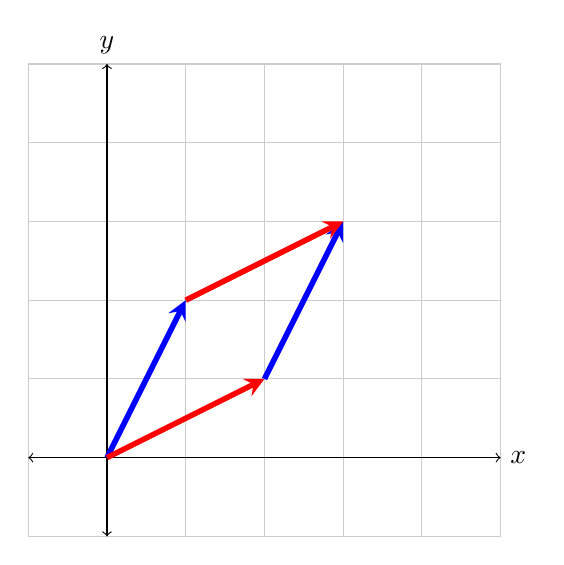
\begin{tikzpicture}
        \draw[thin,gray!40] (-1,-1) grid (5,5);
        \draw[<->] (-1,0)--(5,0) node[right]{$x$};
        \draw[<->] (0,-1)--(0,5) node[above]{$y$};
        \draw[line width=2pt,blue,-stealth](0,0)--(1,2) node[anchor=east] at (.5,1){$\vecu$};
        \draw[line width=2pt, red, -stealth](0,0)--(2,1) node[anchor=north] at (1,.5){$\vecv$};
        \draw[line width=2pt,blue,-stealth](2,1)--(3,3) node[anchor=east] at (.5,1){};
        \draw[line width=2pt, red, -stealth](1,2)--(3,3) node[anchor=north] at (1,.5){};
        \end{tikzpicture}
        \end{center}
        We can then compute the area of this parallelogram by first computing the cross product $\vecu \times \vecv$.  So we have
        \begin{align*}
        \vecu \times \vecv &= (\xhat + 2\yhat)\times(2\xhat + \yhat)\\
        &= 2\xhat \times \xhat + \xhat \times \yhat + 4 \yhat \times \xhat + 2\yhat \times \yhat \\
        &= \zerovec + \zhat - 4\zhat + \zerovec\\
        &= -3\zhat.
        \end{align*}
        Then we have that the area of the parallelogram is
        \[
        \boxed{A = \|\vecu \times \vecv\| = \|-3 \zhat\| = 3.}
        \]
        \end{ex}
        
        \begin{exercise}
        Compute the area of the parallelogram defined by $\vecu=3\xhat + \yhat -\zhat$ and $\vecv=\xhat + 2\yhat -3\zhat$.
        \end{exercise}
        
        %left off editing here...
        %%%%%%%%%%%%%%%%%%%%%%%%%%%%%%%%
        
        \begin{ex}{Angular Velocity and Right-Hand Rule}{angular_velocity}
        For a particle moving along a circle with radius $r$ we can define a quantity called the \emph{angular velocity} and denote it by $\boldsymbol{\vec{\omega}}$.  Then, for example, the time it takes for the particle to travel around the whole circle (the \emph{period}) is
        \[
        \tau = \frac{2\pi r}{\|\boldsymbol{\vec{\omega}}\|}.
        \]
        It turns out that the angular velocity of this particle at any point is given by
        \[
        \boldsymbol{\vec{\omega}}=\frac{\vecr\times \vecv}{\|\boldsymbol{\vec{r}}\|^2}.
        \]
        We can also find $\vecv$ from $\boldsymbol{\vec{\omega}}$ and $\vecr$. Take a look at the figure below and note the orientation of $\boldsymbol{\vec{\omega}}$ relative to the direction the particle travels around the circle.
        \begin{center}
        \begin{figure}[H]
            \centering
            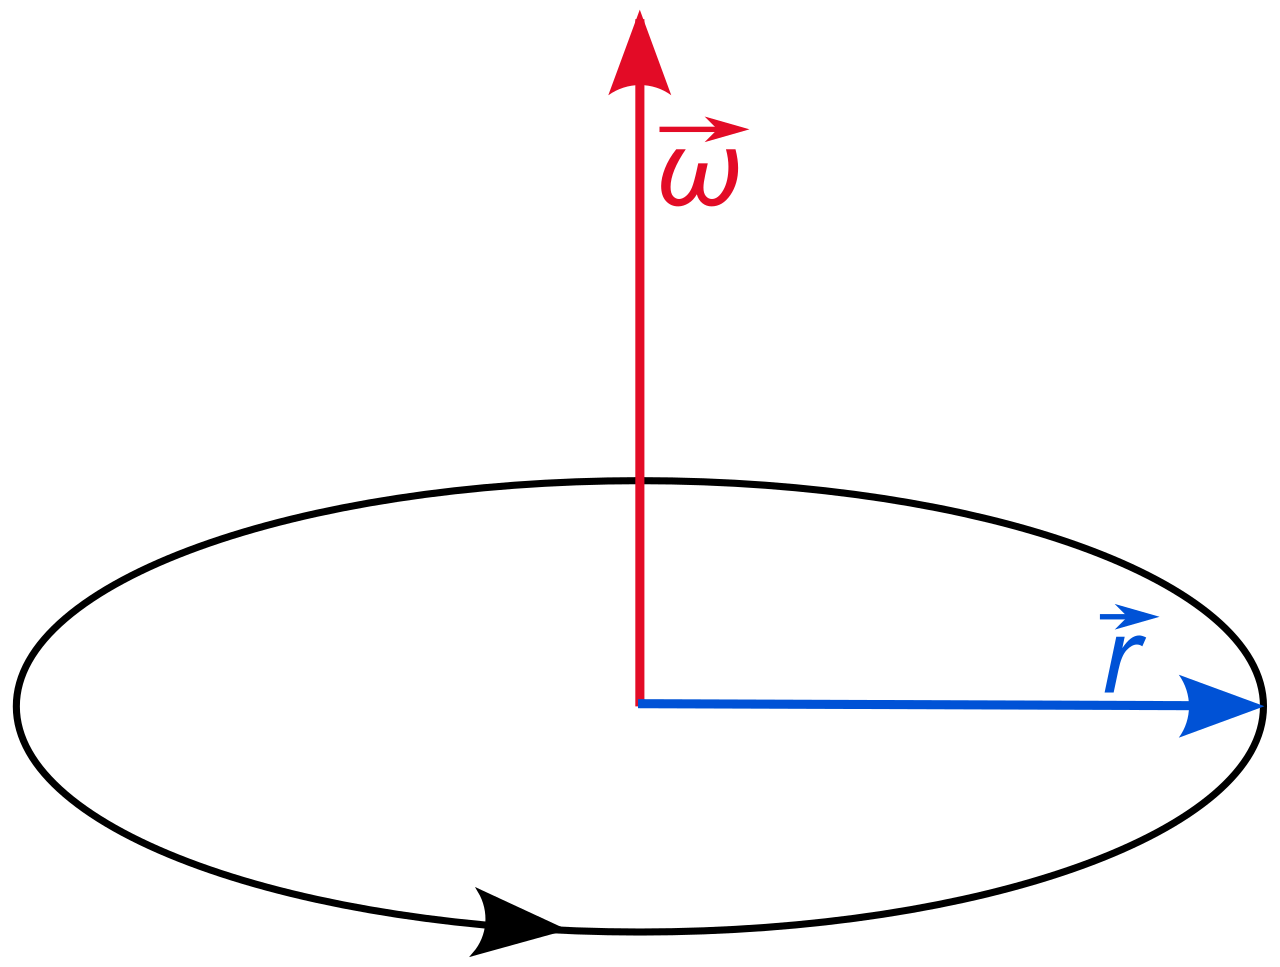
\includegraphics[width=.3\textwidth,bb=0 0 30 30]{Figures/Angular_velocity.png}
            \caption{A particle moving around a circle of radius $\|\vecr\|$ in a counter-clockwise motion.}
            \label{angular-momentum}
        \end{figure}
        \end{center}
        Note that $\vecv$ would be tangent to this circle at the point $\vecr$ and pointing along the direction of travel.
        
        It turns out that $\boldsymbol{\vec{\omega}}$ is a vector pointing perpendicularly to the plane that the circle the particle traverses is in. Which way does $\boldsymbol{\vec{\omega}}$ point? We need the \emph{right-hand rule}!
        \begin{center}
        \begin{figure}[H]
            \centering
            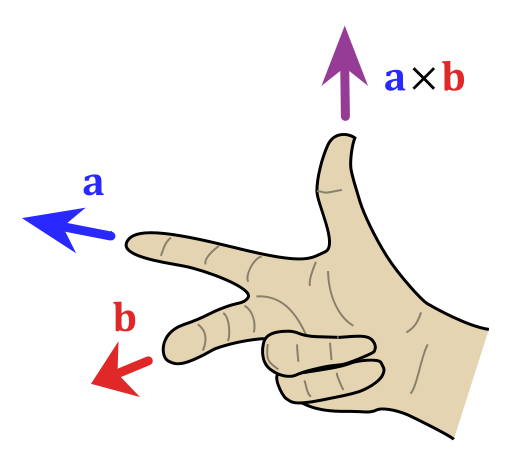
\includegraphics[width=.3\textwidth,bb=0 0 30 30]{Figures/507px-Right_hand_rule_cross_product.png}
            \caption{The right-hand rule.}
        \end{figure}
        \end{center}
        To see how this works, we let $\boldsymbol{\vec{a}}=\vecr$ be our index finger, then $\boldsymbol{\vec{b}}=\vecv$ be our middle finger.  The resulting direction of $\vecr\times \vecv=\boldsymbol{\vec{\omega}}$ is then pointing in the direction we see from Figure \ref{angular-momentum}.
        \end{ex}
        
        
  
        


\chapter{Linear Transformations and Matrices}
        \section{Linear Transformations}
        Now that we have set the stage for vectors and the products between them, we would like to investigate how we can transform these vectors.  Specifically, we will first care about functions that are \emph{linear}.  These will be functions that stretch and rotate vectors and possibly change dimension all while leaving the origin alone.
        
        \begin{df}{Linear Transformation}{linear_transformation}
        A \boldgreen{linear transformation} \index{linear!transformation} is a function
        \[
        T\colon \R^n \to \R^m
        \]
        that satisfies the following requirements:
        \begin{enumerate}[(i)]
            \item $T(\vecu+\vecv)=T(\vecu)+T(\vecv)$,
            \item $T(\alpha \vecv)=\alpha T(\vecv)$,
            \item $T(\zerovec)=\zerovec$.
        \end{enumerate}
        Note that requirement (iii) follows from (i) and (ii), but it is something that is easy to check, so we place it here as well.
        \end{df}
        
        \begin{remark}
        When writing transformations of vectors, we often omit the extra parentheses. That is, instead of
        \[
        T \left( \begin{pmatrix} x \\ y \\ z \end{pmatrix} \right),
        \]
        we will just put
        \[
        T \begin{pmatrix} x \\ y \\ z \end{pmatrix}.
        \]
        \end{remark}
        
        \begin{remark}
        These rules should seem similar to the properties of the derivative and integral.  We'll find that what we're building here will let us properly talk about derivatives in multiple dimensions.
        \end{remark}   
        
        \begin{ex}{Scaling is Linear}{sacaling_linear}
        Consider $T \colon \R^2 \to \R^2$ given by
        \[
        T\begin{pmatrix} x\\ y \end{pmatrix}
        = \begin{pmatrix} \alpha x\\ \beta y \end{pmatrix}.
        \]
        This transformation scales the $x$-component of our vector by $\alpha$ and scales the $y$-component by $\beta$.
        
        To see that this is linear, we just check that it satisfies the three necessary conditions.  First we will show (i). So, if we take two vectors
        \[
        \vecv_1 = \begin{pmatrix} x_1 \\ y_1 \end{pmatrix} \qquad \textrm{and} \qquad \vecv_2 = \begin{pmatrix} x_2 \\ y_2 \end{pmatrix},
        \]
        then we have
        \begin{align*}
        T\left( \vecv_1 + \vecv_2\right)&= T \left( \begin{pmatrix} x_1 \\ y_1 \end{pmatrix} + \begin{pmatrix} x_2 \\ y_2 \end{pmatrix} \right)\\
        &= T\left( \begin{pmatrix} x_1 + x_2 \\ y_1 + y_2 \end{pmatrix} \right)\\
        &= \begin{pmatrix} \alpha(x_1 + x_2) \\ \beta(y_1 + y_2)\end{pmatrix}\\
        &= \begin{pmatrix} \alpha x_1 + \alpha x_2 \\ \beta y_1 + \beta y_2 \end{pmatrix}\\
        &= \begin{pmatrix} \alpha x_1 \\ \beta y_1 \end{pmatrix} + \begin{pmatrix} \alpha x_2 \\ \beta y_2 \end{pmatrix} \\
        &= T(\vecv_1)+T(\vecv_2).
        \end{align*}
        
        Then for (ii), take $\vecv = x\xhat + y\yhat$ and we have
        \begin{align*}
            T(\mu \vecv)&=T\left(\mu \begin{pmatrix} x \\ y \end{pmatrix}\right)\\
            &=T\left( \begin{pmatrix} \mu x \\ \mu y \end{pmatrix}\right)\\
            &= \begin{pmatrix} \alpha \mu x \\ \beta \mu y \end{pmatrix}\\
            &= \mu \begin{pmatrix} \alpha x \\ \beta y \end{pmatrix}\\
            &= \mu T(\vecv).
        \end{align*}
        Since the qualities (i) and (ii) imply (iii), we don't necessarily need to check it. But, we can anyway. So we take
        \begin{align*}
            T(\zerovec)&= T\left(\begin{pmatrix} 0 \\ 0  \end{pmatrix}\right)\\
            &= \begin{pmatrix} \alpha \cdot 0 \\ \beta \cdot 0\end{pmatrix}\\
            &= \zerovec.
        \end{align*}
        So this function $T$ is indeed linear.
        \end{ex}
        
        \begin{exercise}
        Which of the following are linear transformations? Why or why not?
        \begin{enumerate}[(a)]
            \item $f\colon \R \to \R$ given by $f(x)=\lambda x$.
            \item $g\colon \R \to \R$ given by $g(x)=2x+1.$
            \item $h\colon \R \to \R$ given by $h(x)=x^2.$
            \item $T \colon \R^3 \to \R^3$ given by
            \[
            T \begin{pmatrix} x\\ y\\ z \end{pmatrix}  = \begin{pmatrix} y\\ x\\ z \end{pmatrix}.
            \]
        \end{enumerate}
        \end{exercise}
        
        % \begin{ex}{Dot Product is Linear}{dot_prod_linear}
        % If we choose a fixed vector $\mathbf{v}$, then the dot product of another vector $\mathbf{a}$ with $\mathbf{v}$ is itself an example of a linear transformation! It's also a good example of how the input dimension can differ from the output dimension.  Let us write $\textrm{Dot}_\mathbf{v}\colon \R^3 \to \R$ which is given by
        % \[
        % \textrm{Dot}_\mathbf{v}(\mathbf{a})=\mathbf{a}\cdot \mathbf{v}=a_xv_x+a_yv_y+a_zv_z.
        % \]
        % \end{ex}
        
        \begin{exercise}
        Pick a vector in the plane and draw a picture of the scaling transformation.
        \end{exercise}
        
        \begin{ex}{Rotation is Linear}{rot_linear}
        Consider the following linear transformation $T\colon \R^2 \to \R^2$ given by
        \[
        T\begin{pmatrix} x\\ y \end{pmatrix} 
        = \begin{pmatrix} x \cos \theta - y \sin \theta\\ x \sin \theta +y \cos \theta \end{pmatrix} = \begin{pmatrix} x'\\ y' \end{pmatrix}.
        \]
        This transformation rotates a vector by $\theta$ in the counter-clockwise direction. 
        \begin{figure}[H]
            \centering
            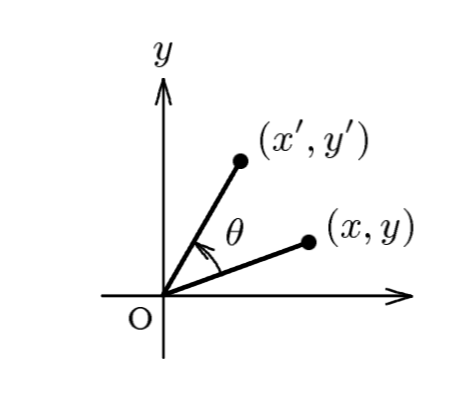
\includegraphics[width=.3\textwidth]{Figures/plane_rotation.png}
        \end{figure}
        \end{ex}
        
    \section{Matrix Representation of Linear Transformations}
        
        The salient fact of linear transformations is how we can represent them.  As it turns out, any linear transformation $T\colon \R^n \to \R^m$ can be written like:
        \[
        T\begin{pmatrix} x_1 \\ x_2 \\ \vdots \\ x_n \end{pmatrix}
        = \begin{pmatrix} y_1 \\ y_2 \\ \vdots \\ y_m \end{pmatrix},
        \]
        where 
        \begin{align*}
            y_1 &= a_{11} x_1 + a_{12} x_2 + a_{13} x_3 + \cdots + a_{1n} x_n\\
            y_2 &= a_{21} x_1 + a_{22} x_2 + a_{23} x_3 + \cdots + a_{2n} x_n\\
            y_3 &= a_{31} x_1 + a_{32} x_2 + a_{33} x_3 + \cdots + a_{3n} x_n\\
            \vdots\\
            y_m &= a_{m1} x_1 + a_{m2} x_2 + a_{m3} x_3 + \cdots + a_{mn} x_n.
        \end{align*}
        Hence, this arbitrary linear transformation is captured entirely by the \boldgreen{matrix} of numbers
        \[
        \begin{pmatrix}
        a_{11} & a_{12} & a_{13} & \cdots & a_{1n}\\
        a_{21} & a_{22} & a_{23} & \cdots & a_{2n}\\
        a_{31} & a_{32} & a_{33} & \cdots & a_{3n}\\
        \vdots & \vdots & \vdots & & \vdots \\
        a_{n1} & a_{n2} & a_{n3} & \cdots & a_{nm}
        \end{pmatrix}
        \]
        
        Now, our study moves to that of matrices since we have seen that matrices capture all that we need in order to describe linear transformations.  They aren't necessary to use, but they make computation and understanding a bit easier.  It turns out that we can also think of vectors as special cases of matrices, which makes the idea of studying matrices themselves all that much better. From here on out, we will restrict ourselves to matrix representations.  
        
        Often, one may be handed a linear transformation $T\colon \R^n \to \R^m$ as above. When one wants to represent $T$ as a matrix, we may put
        \[
        [T]=        \begin{pmatrix}
        a_{11} & a_{12} & a_{13} & \cdots & a_{1n}\\
        a_{21} & a_{22} & a_{23} & \cdots & a_{2n}\\
        a_{31} & a_{32} & a_{33} & \cdots & a_{3n}\\
        \vdots & \vdots & \vdots & & \vdots \\
        a_{n1} & a_{n2} & a_{n3} & \cdots & a_{nm}
        \end{pmatrix}.
        \]
        However, we will often just assume that a linear transformation is given as a matrix a priori.  As one continues to learn more linear algebra, it becomes clear why we wish to make this distinction, but for now this is alright.  In the sequel, we will care about understanding \emph{linear operators} which will not always have some matrix representation.
        
        \subsection{Matrix Algebra}
        Just as we did with vectors, we want to understand what we can do with these matrices algebraically.  These matrices must allow us to perform linear transformations.  Given that linear transformations are special types of functions, we also want to be able to compose linear functions as well.  All that we need will be captured in an algebraic way through matrix multiplication.  
        
        We will call a matrix with $n$-rows and $m$-columns an \textbf{$n\times m$-matrix} (read: $n$ by $m$ matrix).  These take the form:
        \[[A]=
        \begin{bmatrix}
        a_{11} & a_{12} & a_{13} & \cdots & a_{1n}\\
        a_{21} & a_{22} & a_{23} & \cdots & a_{2n}\\
        a_{31} & a_{32} & a_{33} & \cdots & a_{3n}\\
        \vdots & \vdots & \vdots & & \vdots \\
        a_{n1} & a_{n2} & a_{n3} & \cdots & a_{nm}
        \end{bmatrix}.
        \]
        We use a capital letter in brackets to denote a matrix. Each entry of the matrix will be given by a lowercase letter with subscripts $a_{ij}$.  The subscripts will tell you which row and column the entry is located. For example, $a_{25}$ would be the entry in the 2$^\textrm{nd}$ row and $5^\textrm{th}$ column.
        
        \begin{itemize}
            \item \textbf{Equality:} Matrices are equal if each entry is equal. That is, given $\matA$ and $\matB$, we say $\matA=\matB$ if $a_{ij}=b_{ij}$ for each pair $i,j$.  Clearly if these matrices are not the same ``shape" (meaning, they have a different number of rows or columns), then they cannot be the same.  Just as a 2-dimensional vector cannot be the same as a 3-dimensional one.  They are distinctly different objects.
            
            \item \textbf{Addition:} We can add matrices of the same shape.  We write $\matA+\matB=\matC$ and create the new matrix $\matC$ by adding the entries.  That is, $c_{ij}=a_{ij}+b_{ij}$.  
            
            \item \textbf{Scalar Multiplication:} We can also scale matrices.  We do this by scaling the entries.  So, if we have $\alpha \matA=\matB$, then we know the entries of $\matB$ are given by $b_{ij}=\alpha a_{ij}$.
            
            \item \textbf{Matrix Multiplication:} It is also possible to multiply two matrices together.  Recall that matrices are how we capture the information of a linear transformation. Matrix multiplication will capture the idea of composing two linear transformations. Consider two linear transformations
            \[
            A \colon \R^n \to \R^m \qquad \textrm{and} \qquad B \colon \R^m \to \R^p.
            \]
            Then we have that $[A]$ is an $m\times n$-matrix and $[B]$ is a $p\times m$ matrix.  We can create the composite linear transformation 
            \[
            B \circ A \colon \R^n \to \R^p,
            \]
            and hence we would like to understand how to represent this composite function with the two matrices $[A]$ and $[B]$. We define the matrix multiplication
            \[
            [B][A]=[C]
            \]
            to properly capture the composite linear transformation $A\circ B$. Hence, we can multiply matrices $\matA$ and $\matB$ if 
            \[
            \textrm{the number of columns of $\matA$}=\textrm{the number of rows of $\matB$}.
            \]
            If $\matA$ is an $m\times n$-matrix and $\matB$ is an $p\times m$-matrix, then $\matC=\matB \matA$ is an $m\times p$ matrix.  You can remember this helpful fact:
            \[
            (p\times \underbrace{m)\cdot (m}_{\textrm{the same}}\times n)
            \]
            and
            \[
            (\underbrace{p}\times m)\cdot (m\times \underbrace{n})
            \]      
            gives the dimensions of the resulting matrix.
            
            How we perform this matrix multiplication looks a bit ugly at first, but it ends up being slightly easier after digesting this a bit. We have that the components of $\matC=\matB \matA$ are
            \[
            c_{ij}=\sum_{k=1}^m b_{ik}a_{kj}.
            \]
            
            Let us take the example of letting $\matB$ be an $1\times n$-matrix and $\matA$ a $n\times 1$-matrix. Then
            \[
            [B][A]=
            \begin{bmatrix} b_{11} & b_{12} & \cdots & b_{1n}\end{bmatrix}
            \begin{bmatrix} a_{11}\\ a_{21} \\ \vdots \\ a_{n1}\end{bmatrix}=b_{11}a_{11}+b_{12}a_{21}+\cdots+b_{1n}a_{n1}=\sum_{k=1}^n b_{1k}a_{k1}.
            \]
            This is the dot product of two vectors!  As it turns out, we can decompose matrix multiplication into a bunch of dot products. 
            
            In general, if we look at the multiplication described above for the component $c_{ij}$, we can break this down as follows. Note that the $i$th row of a matrix $\matB$ is a vector with $m$ elements, the $j$th column of a matrix $\matA$ is a vector with $m$ elements, and the dot product of these two vectors gives the entry $c_{ij}$ of the matrix $\matB \matA=\matC$.
            \end{itemize}
            
            \begin{remark}
            This all means it is possible to take linear combinations of matrices as well!
            \end{remark}
            
            \begin{prop}{$n\times m$-Matrices Form a Vector Space}{matrix_vspace}
                Let $\mathcal{M}_{n\times m}$ be the set of all $m\times n$-matrices with real or complex entries. Then this set forms a vector space with the scalar multiplication and matrix addition described above.
            \end{prop}
            
            \begin{exercise}
                Show that the above proposition is true.
            \end{exercise}
            
            \begin{ex}{Multiplying Matrices}{multiplying_matrices}
            Let us multiply the following matrices:
            \[
            \matA=\begin{pmatrix} 2 & 0 & -3\\ 1&1&-2\end{pmatrix} \quad \matB=\begin{pmatrix} 2&3&4&1\\1&2&2&0\\0&-1&2&0\end{pmatrix}.
            \]
            Verify that you get
            \[
            \matA \matB=\begin{pmatrix} 4&9&2&2\\3&7&2&1\end{pmatrix}.
            \]
            \end{ex}
            
            \subsection{Properties of Matrix Multiplication}
            
            Matrices will behave in the following ways:
            \begin{itemize}
                \item \textbf{Associativity:} The order in which you choose to multiply matrices does not matter.  That is 
                \[\matA(\matB \matC)=(\matA \matB)\matC=\matA \matB \matC.\]
                \item \textbf{Distributivity:} We can multiply matrices over sums. That is
                \[
                \matA\left(\matB+\matC\right)=\matA \matB+\matA \matC.
                \]
                \item \textbf{(non)-Commutivity:} In general, we have
                \[
                \matA \matB\neq \matB \matA.
                \]
                However, there are certain types of matrices that do commute with each other.
            \end{itemize}
        
        Right now we have the ability to write linear transformations as matrices.  We can also multiply these matrices.  Keep in mind that this in some way mimics composing functions. In essence, we have entirely captured the functional behavior of linear spaces through matrices, since, we can realize vectors as special types of matrices as well.
        
        \section{Systems of Linear Equations}
        Often times we are handed a system of equations to solve.  In this case, we have more than one variable, and the same number of equations is required in order to determine values for these variables uniquely. For example, one may have three equations for the variables $x$, $y$, and $z$ where each equations simultaneously equal zero. That is,
        \begin{align*}
            f(x,y,z) &= 0\\
            g(x,y,z) &= 0\\
            h(x,y,z) &= 0.
        \end{align*}
        In the most general case where $f$, $g$, and $h$ are potentially nonlinear, these equations may be very difficult to solve together.  In the case that each of the above functions is linear, it is much easier to determine a solution (if one exists).
        
        When the equations are linear, we can write them as a matrix times a vector
        \[
        [A]\vecx=\vecy
        \]
        where $A$ is an $n\times m$-matrix, $\vecx$ is an $m$-dimensional vector, and $\vecy$ is an $n$-dimensional vector. In this case, we know the vector $\vecy$, but we wish to determine the correct vector $\vecx$ that satisfies the equation. 
        
        Let us write out what this looks like:
        \[
        \begin{pmatrix}
        a_{11} & a_{12} & \cdots & a_{1m}\\
        a_{21} & a_{22} & \cdots & a_{2m}\\
        \vdots & \vdots & \cdots & \vdots\\
        a_{n1} & a_{n2} & \cdots & a_{nm}
        \end{pmatrix}
        \begin{pmatrix}
        x_1\\ x_2 \\ \vdots \\ x_m
        \end{pmatrix}
        =\begin{pmatrix}
        y_1 \\ y_2 \\ \vdots \\ y_n
        \end{pmatrix},
        \]
        gives us a set of equations
        \begin{align*}
        a_{11} x_1 + a_{12}x_2 + \cdots a_{1m} x_m &= y_1\\
        a_{21} x_1 + a_{22} x_2 + \cdots a_{2m} x_m &= y_2
        &\vdots\\
        a_{n1} x_1 + a_{n2} x_2 + \cdots a_{nm} x_m &= y_n.
        \end{align*}
        We call these equations a \boldgreen{system of linear equations}.
        
        In the most general case for a system of linear equations, it may be that $n\neq m$, and finding solutions is far from guaranteed.  In this case, a system may be \boldgreen{overdetermined} if $n>m$. This is the case where there are more equations than there are variables, hence the name.  When a system is overdetermined, there is likely no solution to the problem. The other case where $n<m$ has fewer equations than the amount of unknown variables in the vector $\vecx$, and we call this system \boldgreen{underdetermined}. When a system is undetermined, we tend to expect a solution, but it won't be unique. 
        
        We will tend to concentrate on the case that is properly determined. That is, we will look at systems of equations that have $n$ equations and $n$ unknowns, which means that $\vecx$ is a vector of length $n$, $\vecy$ is a vector of length $n$, and $[A]$ is an $n\times n$-matrix.
        
        
        \section{Solving Linear Systems of Equations}
        The problem at hand is that we are handed a matrix $[A]$ and an output vector $\vecy$ and we are asked to find a vector $\vecx$ such that the equation
        \[
        [A]\vecx=\vecy
        \]
        is satisfied. If $\vecy$ is equal to the zero vector $\zerovec$, then we call this a \boldgreen{homogeneous} linear system. Otherwise, we call the system \boldgreen{inhomogeneous}.
        
        To solve these equations requires an algorithmic approach. The algorithm we will use is known as \boldgreen{row reduction}. Row reduction is a list of a few rules we are allowed to use in order to modify a matrix and determine a solution to either a homogeneous or inhomogeneous equation.
        
        \begin{df}{Row Operations}{row_operations}
        We call the following list of operations the \boldgreen{elementary row operations}.
        \begin{itemize}
            \item \textbf{Row scaling:} We can scale the rows of a matrix by any scalar value $\alpha$.
            \item \textbf{Row addition:} We can add scalar multiples of any rows to another row.
            \item \textbf{Row swapping:} We can swap any two rows.
        \end{itemize}
        These operations are elementary in the sense that they do not change the ``character" of the matrix.  This means that these will not affect the solution to our system. Also, the operations will make determining the solution doable as well.
        \end{df}
        
        When given a system of linear equations, it becomes handy to shorten what we have to write and place the whole system into a matrix.  However, when we do this, we want to keep separate the matrix $[A]$ from the solution vector $\vecy$. In this matrix, the vector we are solving for, $\vecx$, will not appear. But, when we finish the algorithm, we will have determined $\vecx$.
        
        \begin{df}{Augmented Matrix}{augmented_matrix}
        Given an equation $[A]\vecx=\vecy$, we have the \boldgreen{augmented matrix} \index{augmented matrix} $[M]$. $[M]$ is a matrix with one extra column than $[A]$, and it is created by letting $[A]$ fill the left most columns, and $\vecy$ take the spot in the right most column. For example, for a $3\times3$-matrix $[A]$, and $3$-dimensional vector $\vecy$, we have:
        \[
        [M]=\left(\begin{array}{ccc|c}
        a_{11} & a_{12} & a_{13}  &  y_1 \\
        a_{21} & a_{22} & a_{23} & y_2\\
        a_{31} & a_{32} & a_{33} & y_3
        \end{array}\right).
        \]
        We often use the vertical line to distinguish the output vector $\vecy$ column from the matrix $[A]$ inside of $[M]$.
        \end{df}
        
        Our goal here is to use elementary row operations to reduce our augmented matrix to the following \boldgreen{row reduced echelon form}.  For the example shown in the definition above, this will look like:
        \[
        [M]=\left[\begin{array}{ccc|c}
        1 & 0 & 0  &  x_1 \\
        0 & 1 & 0 & x_2\\
        0 & 0 & 1 & x_3
        \end{array}\right]
        \]
        When we have reduced the augmented matrix to this form, we are able to read off the answer for the vector $\vecx$ as
        \[
        \vecx = \begin{pmatrix} x_1 \\ x_2 \\ x_3 \end{pmatrix}.
        \]
        Thus, the work in solving the linear system just comes down to working in a clever manner with row operations.
        
        \begin{remark}
            Note that not every linear system will have ones allong the diagonal portion as shown above.  It is possible that some of the ones above could be zero, or if we started with a matrix that was not square (i.e., not $n\times n$), then there will be more to deal with.  However, the goal should always be to try and reduce the matrix to this point.
        \end{remark}
        
        \begin{ex}{A System of Inhomogeneous Equations}{system_of_inhomo}
        Let us consider the following matrix equation:
        \[
        \begin{pmatrix}
        1 & 0 & 2\\
        2 & 2 & 3\\
        4 & 4 & 1
        \end{pmatrix}
        \begin{pmatrix}
        x\\
        y\\
        z
        \end{pmatrix}
        =\begin{pmatrix}
        1\\
        1\\
        1
        \end{pmatrix}.
        \]
        If we multiply this out, we get the following system of linear equations:
        \begin{align*}
            1x+0y+2z&=1\\
            2x+2y+3z&=1\\
            4x+4y+1z&=1.
        \end{align*}
        You can solve this by hand, but it is tedious. In fact, each of the tricks you would use to solve this are captured by elementary row operations anyway. So, we will use the row reduction technique instead.  Let us create the augmented matrix
        \[
        \left(\begin{array}{ccc|c}
        1 & 0 & 2 & 1 \\
        2 & 2 & 3 & 1 \\
        4 & 4 & 1 & 1
        \end{array}\right).
        \]
        We can then do row operations on the whole matrix (including the added vector column) to get our result
        \[
        \left(\begin{array}{ccc|c}
        1 & 0 & 2 & 1 \\
        2 & 2 & 3 & 1 \\
        4 & 4 & 1 & 1
        \end{array}\right) \underrightarrow{-2 R_2 \textrm{ from } R_3} 
        \left(\begin{array}{ccc|c}
        1 & 0 & 2 & 1 \\
        2 & 2 & 3 & 1 \\
        0 & 0 & -5 & -1
        \end{array}\right)
        \]
        then
        \[
        \left(\begin{array}{ccc|c}
        1 & 0 & 2 & 1 \\
        2 & 2 & 3 & 1 \\
        0 & 0 & -5 & -1
        \end{array}\right) \underrightarrow{-2 R_1 \textrm{ from } R_2} 
        \left(\begin{array}{ccc|c}
        1 & 0 & 2 & 1 \\
        0 & 2 & -1 & -1 \\
        0 & 0 & -5 & -1
        \end{array}\right).     
        \]
        Now, we can continue,
        \[
        \left(\begin{array}{ccc|c}
        1 & 0 & 2 & 1 \\
        0 & 2 & -1 & -1 \\
        0 & 0 & -5 & -1
        \end{array}\right) \underrightarrow{\div R_3 \textrm{ by }  -5} 
        \left(\begin{array}{ccc|c}
        1 & 0 & 2 & 1 \\
        0 & 2 & -1 & -1 \\
        0 & 0 & 1 & 1/5
        \end{array}\right),    
        \]
        then
        \[
        \left(\begin{array}{ccc|c}
        1 & 0 & 2 & 1 \\
        0 & 2 & -1 & -1 \\
        0 & 0 & 1 & 1/5
        \end{array}\right) \underrightarrow{ +R_3 \textrm{ to }  R_2} 
        \left(\begin{array}{ccc|c}
        1 & 0 & 2 & 1 \\
        0 & 2 & 0 & -4/5 \\
        0 & 0 & 1 & 1/5
        \end{array}\right),    
        \]
        and next
        \[
        \left(\begin{array}{ccc|c}
        1 & 0 & 2 & 1 \\
        0 & 2 & 0 & -4/5 \\
        0 & 0 & 1 & 1/5
        \end{array}\right) \underrightarrow{ \div R_2 \textrm{ by }  2} 
        \left(\begin{array}{ccc|c}
        1 & 0 & 2 & 1 \\
        0 & 1 & 0 & -2/5 \\
        0 & 0 & 1 & 1/5
        \end{array}\right),    
        \]
        and lastly,
        \[
        \left(\begin{array}{ccc|c}
        1 & 0 & 2 & 1 \\
        0 & 1 & 0 & -2/5 \\
        0 & 0 & 1 & 1/5
        \end{array}\right) \underrightarrow{ -2 R_3 \textrm{ from }  R_1} 
        \left(\begin{array}{ccc|c}
        1 & 0 & 0 & 3/5 \\
        0 & 1 & 0 & -2/5 \\
        0 & 0 & 1 & 1/5
        \end{array}\right),    
        \]
        Notice now that this corresponds to the equations
        \begin{align*}
            x+0y+2z&=\frac{3}{5}\\
            0x+y-1z&=\frac{-2}{5}\\
            0x+0y+z&=\frac{1}{5}.
        \end{align*}
        These provide us the answers
        \[
        z=\frac{1}{5} ~\implies~ y=\frac{-2}{5} ~\implies~ x=\frac{3}{5}. 
        \]
        Double check my work above.  But we can also plug in our vector now to verify our result.  That is
        \[
        \begin{pmatrix}
        1 & 0 & 2\\
        2 & 2 & 3\\
        4 & 4 & 1
        \end{pmatrix}
        \begin{pmatrix}
        3/5\\
        -2/5\\
        1/5
        \end{pmatrix}
        =\begin{pmatrix}
        1\\
        1\\
        1
        \end{pmatrix}.        
        \]
        \end{ex}
        
        \begin{remark}
        One should keep in mind that not every system of equations will have a solution. The one above does, but that does not mean that they all will!
        \end{remark}
        
        The case for solving homogeneous systems is slightly different. It turns out that there is an extra \boldgreen{degree of freedom} in the homogeneous equations (when they have a solution).  If one is able to find a solution to a homogeneous equation, then any scalar times that solution vector will also be a solution.  It is also possible to find multiple vectors whose linear combinations are also a solution.
        
        \begin{ex}{System of Homogeneous Equations}{system_of_homo}
        Consider the matrix
        \[
        [A]=\begin{pmatrix}
        2 & 3 & 1\\
        1 & 4 & 3\\
        1 & 2 & 1
        \end{pmatrix}
        \]
        and solve for the vector $\vecx$ so that $[A]\vecx=\zerovec$. Then the augmented matrix is
        \[
        [M]=\left(\begin{array}{ccc|c}
        2 & 3 & 1  &  0 \\
        1 & 4 & 3 & 0\\
        1 & 2 & 1 & 0
        \end{array}\right).
        \]
        Now we can perform row operations.  It will be good to keep track of what you do as I do.
        \[
        \left(\begin{array}{ccc|c}
        2 & 3 & 1  &  0 \\
        1 & 4 & 3 & 0\\
        1 & 2 & 1 & 0
        \end{array}\right) \underrightarrow{-1/2 R_1 \textrm{ from } R_2 \textrm{ and } R_3} 
        \left(\begin{array}{ccc|c}
        2 & 3 & 1  &  0 \\
        0 & 5/2 & 5/2 & 0\\
        0 & 1/2 & 1/2 & 0
        \end{array}\right)
        \]
        \[
        \left(\begin{array}{ccc|c}
        2 & 3 & 1  &  0 \\
        0 & 5/2 & 5/2 & 0\\
        0 & 1/2 & 1/2 & 0
        \end{array}\right) \underrightarrow{-1/5 R_2 \textrm{ from } R_3} 
        \left(\begin{array}{ccc|c}
        2 & 3 & 1  &  0 \\
        0 & 5/2 & 5/2 & 0\\
        0 & 0 & 0 & 0
        \end{array}\right)
        \]
        Notice that the whole last row is all $0$ now.  This corresponds to the equation:
        \[
        0x+0y+0z=0.
        \]
        In this case, we can plug in any value for $x$, $y$, or $z$ and still have a solution.  However, if we look at the other two equations
        \begin{align*}
            2x+3y+1z &=0\\
            \frac{5}{2}y+\frac{5}{2}z&=0,
        \end{align*}
        we can notice that we do have restrictions on the variables.  If we reduce further, we will have
        \[
        \left(\begin{array}{ccc|c}
            1 & 1 & 0 & 0\\
            0 & 1 & 1 & 0\\
            0 & 0 & 0 & 0
        \end{array}\right).
        \]
        Thus we must have that
        \[
        x=-y \qquad \textrm{and} \qquad y=-z.
        \]
        Thus, we can see that choosing a value for $z$ determines the values for the other variables. In this case, we call $z$ a \boldgreen{free variable} since we could choose any value for it. To denote this arbitrary choice for $z$, I'll let $z=t.$  Hence we have that $y=-t$ and $x=t$ which means the solution here is the vector
        \[
        \vecx=\begin{pmatrix} t \\ -t \\ t\end{pmatrix},
        \]
        where $t$ is \emph{any} real number.  Let's check this:
        \[
        \begin{pmatrix}
        2 & 3 & 1\\
        1 & 4 & 3\\
        1 & 2 & 1
        \end{pmatrix}
        \begin{pmatrix}
        t\\
        -t\\
        t
        \end{pmatrix}
        =\begin{pmatrix}
        0\\
        0\\
        0
        \end{pmatrix}.
        \]
        So we are happy.  We found a solution! In fact, we found infinitely many solutions.  It turns out that anything on this \emph{line} is a solution.
        \end{ex}
        
        \begin{remark}
        Note that the zero vector $\zerovec$ is always a solution to homogeneous equations! So we tend to look for \emph{more} solutions than just the zero vector.
        \end{remark}
        
        Finding the homogeneous solutions for a matrix $[A]$ is special enough to warrant a name of its own.  We will also use this terminology later on.
        
        \begin{df}{Nullspace}{nullspace}
            Given a (possibly rectangular) matrix $[A]$, we call the set of all solutions to the homogeneous equation
            \[
            [A]\vecx = \zerovec
            \]
            the \boldgreen{nullspace} of the matrix $[A]$ and denote this by $\Null([A])$.
        \end{df}
        The nullspace of a matrix tells us a lot about the homogeneous solutions to equations with that matrix.  Note that the zero vector $\zerovec$ is always a member of the nullspace for any matrix $[A]$.  If we have that $\Null([A])=\{\zerovec\}$, then we say that the nullspace for $[A]$ is \boldgreen{trivial}.  Also, if we find any set of vectors $\{\vecv_1,\vecv_2,\dots,\vecv_m\}$ is in the nullspace of a matrix $[A]$, then any linear combination of those vectors is in the nullspace as well.
        
        \subsubsection{Systems of Equations as Linear Combinations of Columns}
        There is also another way of thinking about these matrix/vector equations.  If we have, for example, a 3-dimensional system of equations given by
        \[
        [A]\vecx = \vecy
        \]
        then we can think of the columns of $[A]$ as being 3-dimensional vectors. That is, we can put:
        \begin{align*}
            \begin{pmatrix} \vert & \vert & \vert \\ \boldsymbol{\vec{A}}_1 & \boldsymbol{\vec{A}}_2 & \boldsymbol{\vec{A}}_3 \\ \vert & \vert & \vert \end{pmatrix} \begin{pmatrix} x_1 \\ x_2 \\ x_3 \end{pmatrix} &= \begin{pmatrix} y_1 \\ y_2 \\ y_3 \end{pmatrix},
        \end{align*}
        where we have
        \[
            \boldsymbol{\vec{A}}_1 = \begin{pmatrix} a_{11} \\ a_{21} \\ a_{31} \end{pmatrix} \qquad \boldsymbol{\vec{A}}_2 = \begin{pmatrix} a_{12} \\ a_{22} \\ a_{32} \end{pmatrix} \qquad \boldsymbol{\vec{A}}_3 = \begin{pmatrix} a_{13} \\ a_{23} \\ a_{33} \end{pmatrix}.
        \]
        Note that if we perform this multiplication above we have
        \[
        x_1 \boldsymbol{\vec{A}}_1 +x_2 \boldsymbol{\vec{A}}_2  + x_3 \boldsymbol{\vec{A}}_3 = \vecy.
        \]
        So indeed this matrix/vector multiplication is describing how to take a linear combination of the columns of the matrix $[A]$ to obtain the vector $\vecy$.  
        
        \begin{question}
        Is it always possible to obtain the vector $\vecy$ given any matrix $[A]$?
        \end{question}
        
        \begin{answer}
        No, it is not.  We will see a useful tool in the next section that will help us figure out whether this is possible or not.
        \end{answer}
        
    \section{Linear Independence, Span, and Bases}
    
    Say we are looking at the vectors space $\R^3$. What are the smallest sets of vectors that we need in order to create any vector in that space? Clearly, we found that the unit basis vectors $\xhat$, $\yhat$, and $\zhat$ allowed us to do this.  When we read these as column vectors
    \[
    \xhat = \begin{pmatrix} 1 \\ 0 \\ 0 \end{pmatrix} \qquad \yhat = \begin{pmatrix} 0 \\ 1 \\ 0 \end{pmatrix} \qquad \zhat = \begin{pmatrix} 0 \\ 0 \\ 1 \end{pmatrix},
    \]
    this becomes more obvious.  Since if we are given a vector
    \[
    \vecv = \begin{pmatrix} v_x \\ v_y \\ v_z \end{pmatrix},
    \]
    we can put
    \[
    \vecv = v_x \xhat + v_y \yhat + v_z \zhat.
    \]
    However, these unit basis vectors are not the only vectors that we can use to build the vector $\vecv$. This motivates the following two definitions.
    
    \begin{df}{Linearly Independent Vectors}{linear_independence}
        Consider a list of vectors $\{\vecv_1,\vecv_2,\dots,\vecv_m\}$ in the vector space $\R^n$.  We say that the list of vectors is \boldgreen{linearly independent} \index{linearly independent} if
        \[
        \alpha_1 \vecv_1 + \alpha_2 \vecv_2 + \cdots + \alpha_m \vecv_m =\zerovec
        \]
        if and only if each $\alpha_i=0$. If the list of vectors is not linearly independent, we say that it is \boldgreen{linearly depdendent}. \index{linearly dependent}
    \end{df}
    
    It quickly follows that if we are given too many vectors the set must be linearly dependent.  For example, if handed a set of four vectors in the vector space $\R^3$, it is guaranteed that they are linearly dependent. 
    
    \begin{prop}{More Vectors than Dimension}{more_vec_than_dim}
        Consider the list of vectors $\{\vecv_1,\vecv_2,\dots,\vecv_m\}$ in the vector space $\R^m$.  Then if $m>n$, the list of vectors is linearly dependent.
    \end{prop}
    
    The above proposition is similar to why solving underdetermined systems does not have a unique solution. Similarly, if we do not have enough vectors in our list, it may be a linearly dependent list, but we may not be able to form any vector in the space from that list of vectors. This is analogously similar the case of an overdetermined system.  So we would like to know if a list of vectors suffices to generate any vector in the vector space.
    
    \begin{df}{Span}{span}
    Given a list of vectors $S=\{\vecv_1,\vecv_2,\dots,\vecv_m\}$ in the vector space $\R^n$ we say that the \boldgreen{span} of the vectors in the set is all of the possible vectors that can be written as a linear combination of the elements in the set. 
    \end{df}

    When a set of vectors spans the whole space we are interested in, then this suffices to give us a way to build any vector in that space from a linear combination.  We often care to have the smallest set of vectors that does this as well.
    
    \begin{df}{Basis}{basis}
    A \boldgreen{basis} for the vector space $\R^n$ is the smallest list of vectors such that the span of those vectors is $\R^n$.
    \end{df}
    
    It follows that for a space of $n$-dimensions that we must have a basis of $n$-elements. No more, or no less.  That is exactly why we have three unit basis vectors $\xhat$, $\yhat$, and $\zhat$ for the vector space $\R^3$.  
    
    \section{The Determinant and Trace}
    
    Previously we saw matrix vector equations and posed the question in whether the equations or solvable. We also so that it is an equivalent question to ask whether the set of vectors making up a matrix $[A]$ can be put in a linear combination to yield a desired output vector.  In the previous chapter we also explored the geometry of vectors in space and we were able to compute areas and distances.  Now, with one extra tool we will be able to tie all of these concepts together and perform these calculations in arbitrary dimension.
    
    To start, say that we want to compute the area of a parallelogram. Before, we used the cross product to do this, but what will we do if we want to compute volume in higher dimension? Let us explore how we may think of doing this in general.
        
        \begin{ex}{Area of a parallelogram}{area_parallelogram}
        Say we have the vectors
        \[
        \vecu=\begin{pmatrix} 2\\ 0 \end{pmatrix} \quad \vecv=
        \begin{pmatrix} 1\\ 3 \end{pmatrix}.
        \]
        What is the area of the parallelogram that these vectors create? (See previous notes for how the cross product can do this.  We'll see that the cross product is highly related to determinants.)
        
        \begin{center}
        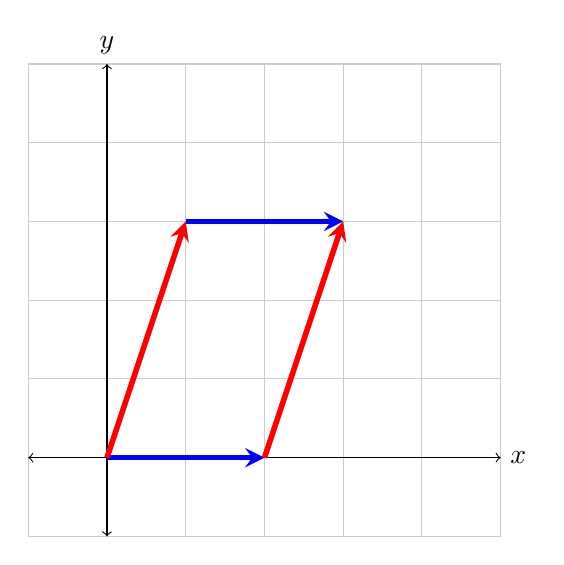
\begin{tikzpicture}
        \draw[thin,gray!40] (-1,-1) grid (5,5);
        \draw[<->] (-1,0)--(5,0) node[right]{$x$};
        \draw[<->] (0,-1)--(0,5) node[above]{$y$};
        \draw[line width=2pt,blue,-stealth](0,0)--(2,0) node[anchor=north] at (1,0){$\vecu$};
        \draw[line width=2pt, red, -stealth](0,0)--(1,3) node[anchor=east] at (.5,1.5){$\vecv$};
        \draw[line width=2pt,red,-stealth](2,0)--(3,3) node[anchor=east] at (.5,1){};
        \draw[line width=2pt, blue, -stealth](1,3)--(3,3) node[anchor=north] at (1,.5){};
        \end{tikzpicture}
        \end{center}
        The trick to finding the area here is to take move a triangle and fill in a gap. We do this like so:
        \begin{center}
        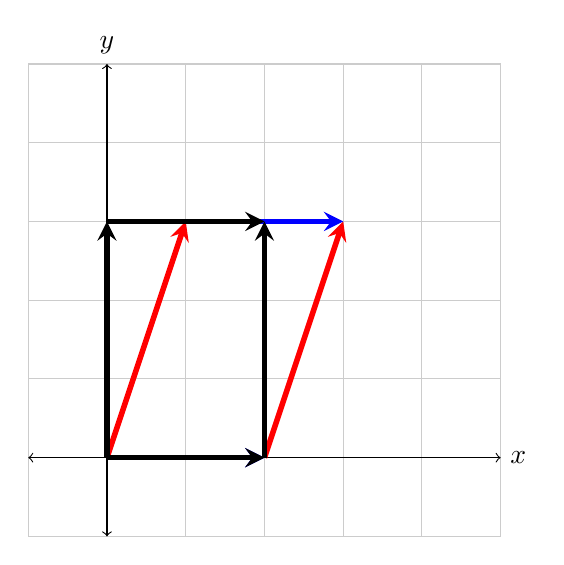
\begin{tikzpicture}
        \draw[thin,gray!40] (-1,-1) grid (5,5);
        \draw[<->] (-1,0)--(5,0) node[right]{$x$};
        \draw[<->] (0,-1)--(0,5) node[above]{$y$};
        \draw[line width=2pt,blue,-stealth](0,0)--(2,0) node[anchor=north] at (1,0){};
        \draw[line width=2pt, red, -stealth](0,0)--(1,3) node[anchor=east] at (.5,1.5){};
        \draw[line width=2pt,red,-stealth](2,0)--(3,3) node[anchor=east] at (.5,1){};
        \draw[line width=2pt, blue, -stealth](1,3)--(3,3) node[anchor=north] at (1,.5){};
        \draw[line width=2pt, black, -stealth](2,0)--(2,3) node[anchor=north] at (1,.5){};    
        \draw[line width=2pt, black, -stealth](0,0)--(0,3) node[anchor=north] at (1,.5){};
        \draw[line width=2pt, black, -stealth](0,0)--(2,0) node[anchor=north] at (1,.5){};
        \draw[line width=2pt, black, -stealth](0,3)--(2,3) node[anchor=north] at (1,.5){};
        \end{tikzpicture}
        \end{center}
        In the above, we've moved a triangle from the right, to the left, to make the black rectangle.  This rectangle then has an area of $2\cdot 3=6.$
        
        Let us see the way we can do this that does not require this extra work.  Let us place these vectors into a matrix:
        \[
        A=\begin{pmatrix} \vert & \vert \\ \vecu & \vecv \\ \vert & \vert \end{pmatrix}=
        \begin{pmatrix} 2 & 1\\ 0 & 3 \end{pmatrix}.
        \]
        Then $\det(A)$ will give us the area of this parallelogram! We have
        \[
        \det(A)=2\cdot 3 - 1\cdot 0 = 6.
        \]
        This begs the question, what is this formula in general? Note, that if you placed these vectors in $\R^3$ by adding a zero $z$-component, then 
        \[
        \|\vecu \times \vecv \| = 6,
        \]
        as well.
        \end{ex}
        
        In order to move to higher dimensions we must first settle the case in two dimensions.  So, to compute the \boldgreen{determinant} of a $2\times 2$-matrix
        \[
        [A]=\begin{pmatrix} a & b\\ c & d \end{pmatrix},
        \]
        we have
        \[
        \det([A]) = ad-bc.
        \]
        You can remember this by thinking that you multiply top left with bottom right, then subtract the product of top right with bottom left. Also, we will often use the notation of vertical bars around the matrix of numbers to denote a determinant. That is,
        \[
        \det([A]) = \left| \begin{matrix} a & b \\ c & d \end{matrix} \right|.
        \]
        
        Now, the generalization of a parallelogram to 3-dimensional space is called a \boldgreen{parralelepiped}.  Later on when we are doing calculus in 3-dimensional space it will become extremely important to be able to compute infinitesimal volumes (just like we have infinitesimal lengths $dx$) and they will be found via the volume of a parallelepiped.
        
        \begin{ex}{Volume of a Parallelepiped}{volume_of_parallelepiped}
        In $3$-dimensional space, we can take three vectors
        \[
        \vecu=\begin{pmatrix} 0 \\ 3 \\ 0 \end{pmatrix}\qquad
        \vecv=\begin{pmatrix} 1 \\ 0 \\ 0 \end{pmatrix}\qquad
        \vecw=\begin{pmatrix} 0 \\ 0 \\ 2 \end{pmatrix}.
        \]
        These, when combined properly, enclose a volume of a parallelepiped. 
\begin{center}
\tdplotsetmaincoords{60}{120} 
\begin{tikzpicture} [scale=3, tdplot_main_coords, axis/.style={->,black,thick}, 
vector/.style={-stealth,blue,very thick}, 
vector guide/.style={dashed,red,thick}]

%standard tikz coordinate definition using x, y, z coords
\coordinate (O) at (0,0,0);

%tikz-3dplot coordinate definition using x, y, z coords

\pgfmathsetmacro{\ax}{0.6}
\pgfmathsetmacro{\ay}{1}
\pgfmathsetmacro{\az}{0.8}

\coordinate (P) at (\ax,\ay,\az);

%draw axes
\draw[axis] (0,0,0) -- (1,0,0) node[anchor=north east]{$x$};
\draw[axis] (0,0,0) -- (0,1,0) node[anchor=north west]{$y$};
\draw[axis] (0,0,0) -- (0,0,1) node[anchor=south]{$z$};


\draw[line width=2pt, red, -stealth](0,0,0)--(0,3/4,0) node[anchor=north west] at (0,3/4,0){$\vecu$};
\draw[line width=2pt, blue, -stealth](0,0,0)--(1/4,0,0) node[anchor=north] at (1/4,0,0){$\vecv$};
\draw[line width=2pt, green, -stealth](0,0,0)--(0,0,1/2) node[anchor=east] at (0,0,1/2){$\vecw$};

\end{tikzpicture}
\end{center}
\begin{center}
\tdplotsetmaincoords{60}{120} 
\begin{tikzpicture} [scale=3, tdplot_main_coords, axis/.style={->,black,thick}, 
vector/.style={-stealth,blue,very thick}, 
vector guide/.style={dashed,red,thick}]

%standard tikz coordinate definition using x, y, z coords
\coordinate (O) at (0,0,0);

%tikz-3dplot coordinate definition using x, y, z coords

\pgfmathsetmacro{\ax}{0.6}
\pgfmathsetmacro{\ay}{1}
\pgfmathsetmacro{\az}{0.8}

\coordinate (P) at (\ax,\ay,\az);

%draw axes
\draw[axis] (0,0,0) -- (1,0,0) node[anchor=north east]{$x$};
\draw[axis] (0,0,0) -- (0,1,0) node[anchor=north west]{$y$};
\draw[axis] (0,0,0) -- (0,0,1) node[anchor=south]{$z$};


\draw[line width=2pt, red, -stealth](0,0,0)--(0,3/4,0) node[anchor=north west] at (0,1,0){};
\draw[line width=2pt, blue, -stealth](0,0,0)--(1/3,0,0) node[anchor=north] at (1/3,0,0){};
\draw[line width=2pt, green, -stealth](0,0,0)--(0,0,1/2) node[anchor=east] at (0,0,2/3){};

\draw[line width=2pt, red, -stealth](1/4,0,0)--(1/4,3/4,0) node[anchor=north west] at (1/3,2/3,3/3){};
\draw[line width=2pt, blue, -stealth](0,3/4,0)--(1/4,3/4,0) node[anchor=north] at (1/3,0,0){};
\draw[line width=2pt, green, -stealth](1/4,0,0)--(1/4,0,1/2) node[anchor=east] at (0,0,2/3){};

\draw[line width=2pt, red, -stealth](1/4,0,1/2)--(1/4,3/4,1/2) node[anchor=north west] at (1/3,2/3,3/3){};
\draw[line width=2pt, blue, -stealth](0,0,1/2)--(1/4,0,1/2) node[anchor=north] at (1/3,0,0){};
\draw[line width=2pt, green, -stealth](0,3/4,0)--(0,3/4,1/2) node[anchor=east] at (0,0,2/3){};

\draw[line width=2pt, red, -stealth](0,0,1/2)--(0,3/4,1/2) node[anchor=north west] at (1/3,2/3,3/3){};
\draw[line width=2pt, blue, -stealth](0,3/4,1/2)--(1/4,3/4,1/2) node[anchor=north] at (1/3,0,0){};
\draw[line width=2pt, green, -stealth](1/4,3/4,0)--(1/4,3/4,1/2) node[anchor=east] at (0,0,2/3){};
\end{tikzpicture}
\end{center}
Of course, I picked an easy example for the illustration.  But what is the volume? Here we again know we can compute this the usual way and we get that the volume is $1\cdot 1 \cdot 2 = 2.$ If we instead created a more complicated paralleliped like: 
\begin{figure}[H]
  \centering
  \includesvg[width=.4\textwidth]{Figures_Part_4/Parallelepiped.svg}
  \label{fig:paralellepiped}
\end{figure}
we must perform the same type of process as we did in Example \ref{ex:area_parallelogram}. The determinant is designed to do this process for us.
\end{ex}

Now, let us consider computing the determinant for a $3\times 3$-matrix $[A]$.  We should think of this matrix as being created from three vectors $\colA_1$, $\colA_2$, and $\colA_3$ as columns. So we have
\[
[A]=\begin{pmatrix} a_{11} & a_{12} & a_{13} \\ a_{21} & a_{22} & a_{23} \\ a_{31} & a_{32} & a_{33}  \end{pmatrix} =
\begin{pmatrix} \vert & \vert & \vert \\ \colA_1 & \colA_2 & \colA_3 \\ \vert & \vert & \vert \end{pmatrix},
\]
we want $\det(A)$ to reflect the the volume of a parallelepiped generated by $\colA_1$, $\colA_2$, and $\colA_3$. It turns out the way we compute $\det(A)$ comes from using the determinant of $2\times 2$-matrices.  Let me explain further.

Let me write this matrix as a tool:
\[
\begin{pmatrix} + & - & +\\ - & + & - \\ + & - & + \end{pmatrix}.
\]
What we will use this for is a memory tool when we do something called the \boldgreen{cofactor expansion}.  What I will do is choose a row or column to expand along.  For this example, let's choose the top row to expand along.  If we use this above matrix with pluses and minuses, we note that the top row will have signs $+-+$. These signs show up in our computation. We will also have to take into account the element in the original matrix and multiply by that.

We start with the top left of $[A]$ and we will have a $+$ sign.  The top left of $[A]$ is element $a_{11}$ and so we remove the first row and first column from $[A]$ to give the \boldgreen{cofactor matrix}
\[
\textrm{Cof}_{11}[A]=\begin{pmatrix} a_{22} & a_{23} \\ a_{32} & a_{33} \end{pmatrix}.
\]
Since ths is a $2\times2$-matrix, we can compute the determinant by \[
\det(\textrm{Cof}_{11})[A])=a_{22} a_{33}- a_{23} a_{32}.
\]
Then we continue expanding along this row and move on to the top middle of $[A]$ and will have a $-$ sign. The top middle element is $a_{12}$ and so we remove the first row and second column of $[A]$ to get
\[
\textrm{Cof}_{12}[A]=\begin{pmatrix} a_{21} & a_{23} \\ a_{31} & a_{33}\end{pmatrix}.
\]
Then we have that 
\[
\det(\textrm{Cof}_{12}[A])=a_{21}a_{33}-a_{31}a_{13}.
\]
Lastly, we move on to the top right of $[A]$ and will have a $+$ sign. The top right element is $a_{13}$ and so we remove the first row and third column of $[A]$ to give
\[
\textrm{Cof}_{13}[A]=\begin{pmatrix} a_{21} & a_{22} \\ a_{31} & a_{32} \end{pmatrix}.
\]
Then we have that
\[
\det(\textrm{Cof}_{13}[A])=a_{21}a_{32} - a_{22}a_{31}.
\]
We then define the determinant of $[A]$ to be
\[
\det([A]) = +a_{11} \det(\textrm{Cof}_{11}[A]) - a_{12} \det(\textrm{Cof}_{12}[A]) + a_{13} \det(\textrm{Cof}_{13}[A]).
\]
Similarly, if we expanded along the second column, for example, we would have that
\[
\det([A]) = -a_{12} \det(\textrm{Cof}_{12}[A]) + a_{22} \det(\textrm{Cof}_{22}[A]) - a_{32} \det(\textrm{Cof}_{32}[A]).
\]

\begin{ex}{Volume of a Parallelepiped from the Determinant}{vol_paralellepiped_from_det}
 Consider the vectors from the previous example
 \[
 \vecu = \begin{pmatrix} 0 \\ 3 \\ 0 \end{pmatrix} \qquad \vecv = \begin{pmatrix} 1 \\ 0 \\ 0 \end{pmatrix} \qquad \vecw = \begin{pmatrix} 0 \\ 0 \\ 2 \end{pmatrix}.
 \]
 Then we can place these three vectors into a matrix $[A]$ by
 \[
 [A]=\begin{pmatrix} \vert & \vert & \vert \\ \vecu & \vecv & \vecw \\ \vert & \vert & \vert \end{pmatrix} = \begin{pmatrix} 0 & 1 & 0 \\ 3 & 0 & 0 \\ 0 & 0 & 2 \end{pmatrix}.
 \]
 Then we can compute the determinant of $[A]$ by expanding along any row or column.  Typically, one wants to expand along a row or column with the most zeros. This will reduce the amount of work.  Here, it does not matter, so let us expand across the top row. We get
 \begin{align*}
 \det([A]) &= a_{11} \det(\textrm{Cof}_{11}[A]) - a_{12} \det(\textrm{Cof}_{12}[A]) + a_{13} \det(\textrm{Cof}_{13}[A])\\
 &=0\cdot \left| \begin{matrix} 0 & 0 \\ 0 & 2 \end{matrix} \right| - 1 \cdot \left| \begin{matrix} 3 & 0 \\ 0 & 2 \end{matrix} \right| + 0 \cdot \left| \begin{matrix} 3 & 0 \\ 0 & 0 \end{matrix} \right|\\
 &= -1 \cdot(3\cdot 2)\\
 &= -6.
 \end{align*}
 This determinant gave us exactly the negative of the volume of the parallelepiped. 
\end{ex}

From the previous example we saw that the determinant need not always be positive.  So we must say that the determinant of a matrix $[A]$ provides us the \boldgreen{signed volume} of the paralellepiped generated by its column vectors. The orientation is much like the orientation we saw for the cross product.


        \begin{exercise} Let
        \[
        A=\begin{pmatrix} 1 & 2 & 3 \\ 4 & 5 & 6 \\ 7 & 8 & 9 \end{pmatrix}.
        \]
        \begin{enumerate}[(a)]
            \item Find $\textrm{Cof}_{11}(A)$.
            \item Find $\textrm{Cof}_{22}(A)$.
            \item Find $\textrm{Cof}_{23}(A)$.
            \item Compute $\det(A)$.
        \end{enumerate}
        
        \end{exercise}
        
        \begin{question}
        What does it mean if $\det(A)=0$ for some matrix $A$?
        \end{question}
        
        \begin{answer}
        It means that we have a parallelopiped with zero volume.  Which means our three vectors actually lie in a plane, or even on a single line.  This is an important fact that will come up when we solve systems of equations!
        \end{answer}
        
        \begin{remark}
        Determinants can be computed in arbitrary dimension using the same process above. But, this will not be a worry for us at the moment.
        \end{remark}
        
        \subsection{Determinants and Systems of Equations}
    
    In defining the determinant, we found it useful for computing the volume of a parallelepiped. However, it does not stop there. If we adopt the convention that systems of linear equations such as
    \[
    [A]\vecx = \vecy
    \]
    where $[A]$ is a square matrix, then this is related to the question of whether the columns of $[A]$ form a spanning list of vectors for the vector space. 
    
    Since the determinant $\det([A])$ tells us the volume of the paralellepiped of the three column vectors creating $[A]$, if the volume is zero, then we know that the columns of $[A]$ must be linearly dependent. Since, if they were nonzero, the vectors would generate some volume.  Thus we have the following two propositions.
    
    \begin{prop}{Solutions to Homogeneous Equations}{solutions_to_homo}
        Consider the homogeneous equation
        \[
        [A]\vecx = \zerovec.
        \]
        Then we have the solutions:
        \begin{itemize}
            \item (Trivial) The only solution for $\vecx$ is $\vecx=\zerovec$ if and only if $\det(A)\neq 0$;
            \item There are multiple nonzero solutions for $\vecx$ if and only if $\det(A)= 0$.
        \end{itemize}
        \end{prop}
        
        The other way of wording the above proposition is that a matrix $[A]$ with a nonzero determinant equal has a nullspace that is trivial. In other words, if 
        \[
        \det([A])= 0
        \]
        then $\Null([A])=\{\zerovec\}$.  Otherwise, if the determinant is zero, then $\Null([A])$ contains more than just the zero vector. 
        
        There is a similar result for the inhomogeneous equations as well.  However, be careful to note the differences here. Afterwards we can discuss geometrically what is happening.
        
        \begin{prop}{Solutions to Inhomogeneous Equations}{solutions_to_inhomo}
        The inhomogenous equation
        \[
        [A]\vecx = \vecy
        \]
        (with $\vecy\neq \zerovec)$ have the following solutions:
        \begin{itemize}
            \item A unique solution for $\vecx$ if and only if $\det(A)\neq 0$;
            \item None or possibly infinitely many solutions for $\vecx$ if $\det(A)=0$.
        \end{itemize}
        \end{prop}
        
    \begin{exercise}
        Take the determinant and then attempt to solve the following homogeneous equations.
        \begin{enumerate}[(a)]
            \item Let 
            \[
            [A]=\begin{pmatrix}
            1 & 1 & 0\\
            1 & 0 & 5\\
            0 & 1 & 2
            \end{pmatrix}
            \]
            and solve $A\vecx=\zerovec.$
            \item Let
            \[
            [B]=\begin{pmatrix}
            2 & 3 & 1\\
            1 & 4 & 3\\
            1 & 2 & 1
            \end{pmatrix}
            \]
            and solve $[B]\vecx=\vecy.$
        \end{enumerate}
        \end{exercise}
        
        When thinking about these propositions, one should consider the case for functions $f\colon \R\to \R$.  In this case, we may have been handed a function $f$, a $y$ (output) value, and were asked to find what input $x$ corresponds to that $y$ value. That is, we want
        \[
        f(x)=y.
        \]
        Here we could sometimes find an inverse function $f^{-1}$ that would satisfy
        \[
        f^{-1}(y)=x.
        \]
        However, for example, if we had the function $f(x)=x^2$, then there was no inverse function.  Why? Well, say we let $y=1$, then $x=\pm 1$ are both solutions. This is not a valid function (since it does not pass the vertical line test). Also, if we provide $y=-1$, then there is no input value to achieve that output.
        
        We can also think of solving systems of linear equations in a geometrical way.  Let us consider two examples.  First, for the homogeneous case, we can take the homogeneous equation
        \[
        \begin{pmatrix} 1 & 0 & 0 \\ 0 & 1 & 0 \\ 0 & 0 & 0 \end{pmatrix} \begin{pmatrix} x \\ y \\ z \end{pmatrix} = \begin{pmatrix} 0 \\ 0 \\ 0 \end{pmatrix}.
        \]
        Here we can see that this gives the equations
        \[
        x=1,\qquad y=1,\qquad z=t.
        \]
        That is, $z$ is a free variable.  Hence here we find that the nullspace for the matrix 
        \[
        [A]=\begin{pmatrix} 1 & 0 & 0 \\ 0 & 1 & 0 \\ 0 & 0 & 0 \end{pmatrix}
        \]
        is given by
        \[
        \Null([A])=\Span\left( \begin{pmatrix} 0 \\ 0 \\ 1 \end{pmatrix}\right),
        \]
        which is the $z$-axis. If we think of columns of $[A]$ as vectors, then we find that the span of the columns is the $xy$-plane.  Thus, any $z$-component of an input vector does not affect the output.
        
        If we take this same matrix at consider an inhomogeneous problem, then the following equation has no solution
        \[
        \begin{pmatrix} 1 & 0 & 0 \\ 0 & 1 & 0 \\ 0 & 0 & 0 \end{pmatrix} \begin{pmatrix} x \\ y \\ z \end{pmatrix} = \begin{pmatrix} 0 \\ 0 \\ 1 \end{pmatrix}.        
        \]
        Why is that? Well, this gives rise to the equations
        \[
        x=1,\qquad y=1, \qquad 0\cdot z = 1,
        \]
        which has no solution for $z$.  This is exactly because of the fact that the columns of $[A]$ only span the $xy$-plane.  Taking a linear combination of the columns cannot give a resulting vector with a $z$-component.  We can visualize this as follows.  Let
        \[
        [T]=\begin{pmatrix} 1 & 0 & 0 \\ 0 & 1 & 0 \\ 0 & 0 & 0 \end{pmatrix} \qquad \textrm{and} \qquad \vecv = \begin{pmatrix} x \\ y \\ z \end{pmatrix},
        \]
        and we can see geometrically what this transformation does to a vector.  In a sense, this transformation removes a whole dimension from $\R^3$. It takes any $z$-component and removes it, hence we see that the transformation really takes the shadow of the input vector on the $xy$-plane.
        \begin{figure}[H]
            \centering
            \includesvg[width=.7\textwidth]{Figures_Part_4/linear_transform_kernel.svg}
        \end{figure}
        That is, we visually see that
        \[
        [T]\vecv = \begin{pmatrix} x \\ y \\ 0 \end{pmatrix}.
        \]
        
        Though this was a special circumstance, this is the exact picture to have in mind when solving systems of linear equations.  If we are given a point $\vecy$, a matrix $[A]$, and are asked to find the input vector $\vecx$ that solves
        \[
        [A]\vecx = \vecy,
        \]
        we are being asked if $\vecy$ is in the span of the columns of $[A]$ and $\vecx$ describes the coefficients for this linear combination.  And as we have seen, the columns of $[A]$ may or may not span the necessary amount of space to be able to create the output vector $\vecy$.
        
        The cross product and the determinant are related in some ways.  Since the formula for a cross product is not easy to memorize, and applying the cross product to basis vectors is tedious, it suffices to remember how to compute determinants of $3\times 3$-matrices and stop there. It is possible to compute the cross product by using the proper determinant. 
        
        \begin{ex}{Cross product from the Determinant}{cross_prod_det}
        You can compute the cross product from the determinant.  (You should be warned: this is an abuse of notation and a somewhat weird coincidence.) Let us create choose two vectors $\mathbf{v}$ and $\mathbf{w}$. We place them in a matrix $[A]$ as follows:
        \[
        A=
        \begin{bmatrix}
        \xhat & \yhat & \zhat\\
        v_x & v_y & v_z\\
        w_x & w_y & w_z
        \end{bmatrix}.
        \]
        Then $\det([A])$ will give us the cross product $\mathbf{v}\times \mathbf{w}$.  Just know that you are briefly ignoring the fact that $\xhat$, $\yhat$, $\zhat$ are actually vectors when you compute this.  Treat them as numbers until you get your final result.
        \end{ex}
        
        
        \subsection{Properties of determinants}
        There are a few nice properties of determinants to keep in mind. 
        \begin{itemize}
            \item \textbf{Transposition:} If we exchange rows for columns in a matrix (that is, to take the \emph{transpose matrix}, then the value of the determinant is the same. Given
            \[
            [A]=\begin{pmatrix}
            a_{11} & a_{12} & a_{13}\\
            a_{21} & a_{22} & a_{23}\\
            a_{31} & a_{32} & a_{33}
            \end{pmatrix}
            \]
            we write the transpose matrix
            \[
            [A]^T=\begin{bmatrix}
            a_{11} & a_{21} & a_{31}\\
            a_{12} & a_{22} & a_{32}\\
            a_{13} & a_{23} & a_{33}
            \end{bmatrix}.
            \]
            So $a_{ij}\mapsto a_{ji}$. Then
            \[
            \det([A])=\det([A]^T).
            \]
            
            \item \textbf{Multiplication by constants:} If we multiply a row or column by a scalar, then the determinant is also multiplied by that scalar.  So we have
            \[
            [A]_\alpha=\begin{bmatrix}
            \alpha a_{11} & \alpha a_{12} & \alpha a_{13}\\
            a_{21} & a_{22} & a_{23}\\
            a_{31} & a_{32} & a_{33}
            \end{bmatrix}
            \]
            Then
            \[
            \det([A]_\alpha)=\alpha \det([A]).
            \]
            And this holds no matter what row or column we scale.
            
            \item \textbf{Linear combinations of rows or columns:} If  we add a linear combination of columns (or rows) to any column (or row), then the determinant does not change. That is, if we have
            \[
            [A] = \begin{pmatrix} \vert & \vert & \vert \\ \colA_1 & \colA_2 & \colA_3 \\ \vert & \vert & \vert \end{pmatrix},
            \]
            then
            \[
            det([A]) = \left| \begin{matrix} \vert & \vert & \vert \\ \colA_1+\alpha\colA_2+\beta\colA_2 & \colA_2 & \colA_3 \\ \vert & \vert & \vert \end{matrix}\right|.
            \]
            Here we just showed adding a linear combination of two columns to the first column, but this holds in general for adding linear combinations of any columns to other columns or adding linear combinations of rows to any row.
            \item \textbf{Exchanging rows or columns:} If we swap rows or columns, the determinant is multiplied by $-1$. So we have
            \[
            \left|\begin{array}{ccc}
                a_{11} & a_{12} & a_{13} \\
                a_{21} & a_{22} & a_{23} \\
                a_{31} & a_{32} & a_{33}
            \end{array}\right|=-
            \left|\begin{array}{ccc}
                a_{12} & a_{11} & a_{13} \\
                a_{22} & a_{21} & a_{23} \\
                a_{32} & a_{31} & a_{33}
            \end{array}\right|
            \]
            Again, this holds for swapping any two rows (or any two columns).
            
            \item \textbf{Linearly-dependent rows or columns:} If a column (resp. row) of a matrix can be written as a linear combination of the other two columns (resp. rows), then the determinant is zero.  This is basically saying that all three vectors lie in a single plane and so the volume of the parallelepiped given by the three vectors (as columns in the matrix) create no volume.
            
            Say we can write
            \[
            \colA_1 = \alpha \colA_2 + \beta \colA_3
            \]
            Then $\det(A)=0.$ That is, if one column (or row) is in the span of the other columns (or rows), then the determinant of the matrix will be zero.
        \end{itemize}
        
        Another nice property of the determinant comes from the product of two matrices.  If we consider two square $n\times n$-matrices $[A]$ and $[B]$, then we can multiply both $[A]$ and $[B]$. Then we have that the determinant is \boldgreen{multiplicative} in that
        \[
        \det([A][B])=\det([A])\det([B]).
        \]
        This turns out to be a very useful property of the determinant.  If one thinks of the determinant as describing how much the basis vectors $\xhat$, $\yhat$, and $\zhat$ are stretched by the composition transformation $[A][B]$, then this is saying that the product transformation stretches the vectors by first stretching by $[A]$ then by $[B]$.
        
        \subsection{The Trace}
        
        The determinant was an example of an \boldgreen{invariant} of a matrix $[A]$. That is, it is a quantity that does not change even when certain operations are performed. These operations that leave the determinant invariant were the row operations.
        
        Given a square matrix $[A]$, we can associate to it another invariant called the \boldgreen{trace} which is rather easy to compute.  The trace of a matrix is simply the sum of the diagonal entries. That is, given
        \[
        [A]=\begin{pmatrix} a_{11} & a_{12} & a_{13} \\ a_{21} & a_{22} & a_{23} \\ a_{31} & a_{32} & a_{33} \end{pmatrix}
        \]
        then the trace of $[A]$ is
        \[
        \tr([A]) = a_{11}+a_{22}+a_{33} = \sum_{i=1}^3 a_{ii}.
        \]
        
        \begin{ex}{Trace of a Matrix}{trace_of_matrix}
        Consider the matrix
        \[
        [A]=\begin{pmatrix} 1 & 2 & 3 \\ 4 & 5 & 6 \\ 7 & 8 & 9 \end{pmatrix}.
        \]
        Then we have
        \[
        \tr([A])=1 + 5 + 9 = 15.
        \]
        \end{ex}
        
        The trace has a few nice properties as well. First, the trace is \boldgreen{additive} so that if we have two $n\times n$-matrices $[A]$ and $[B]$ then 
        \[
        \tr([A]+[B]) = \tr([A]+[B]).
        \]
        However, the trace is not multiplicative like the determinant!  
        
        But, if we have a product of matrices $[A]$, $[B]$, and $[C]$, then we have
        \[
        \tr([A][B][C])=\tr([B][C][A])=\tr([C][A][B]),
        \]
        which is a way of saying that we can \boldgreen{cyclically permute} products of matrices with the trace. For a product of two matrices this means
        \[
        \tr([A][B])=\tr([B][A]).
        \]
        
        Lastly, if we scale a matrix by a constant, then that scales the trace by a constant as well. That is,
        \[
        \tr(\alpha[A])=\alpha \tr([A]).
        \]
        
        The invariant actions for the trace are a require a bit more knowledge that we will develop in the next section.
        
    \section{Inverse Matrices and Similarity }
        As previously mentioned, we can be handed an equation such as
        \[
        f(x)=y,
        \]
        and attempt to find an inverse function $f^{-1}$ so that we have
        \[
        f^{-1}(y)=x.
        \]
        This is generally a very useful tactic to use.  In this case, we can quickly find an input $x$ for a given $y$ without having to solve a new set of equations each time.
        
        Since matrices are representations of linear functions, we can attempt to find an inverse for matrices as well.  If we are given the equation
        \[
        [A]\vecx=\vecy,
        \]
        then we can try to determine the matrix $[A]^{-1}$ so that
        \[
        \vecx = [A]^{-1}\vecy.
        \]
        Hence, if we are given any output vector $\vecy$, we can quickly find the corresponding input vector $\vecx$ through matrix multiplication. We call this special matrix $[A]^{-1}$ the \boldgreen{inverse matrix}\index{inverse!matrix}. In this case $[A]$ \underline{must} be square or else this is not at all possible! If a given matrix $[A]$ has an inverse matrix we say that $[A]$ is \boldgreen{invertible}\index{invertible}.
        
        Since $[A]$ is a function (specifically, a linear transformation), we do not always have an inverse. However, the determinant carries enough data to tell us when a matrix is invertible.  Suppose that $[A]$ is an $n\times n$-matrix, it turns out that $[A]^{-1}$ exists when the columns of $[A]$ span $\R^n$.  Based on our knowledge of the determinat, we can phrase this another way.
        
        \begin{prop}{Existence of Inverse}{existence_of_inverse}
        If $\det([A])\neq 0$, then $[A]^{-1}$ exists and is unique.
        \end{prop}
        
        When speaking of inverses, we must also realize what function acts as the \boldgreen{identity}\index{identity}.  For example, if we have a function $f(x)=y$ that is invertible. Then we know
        \[
        f(f^{-1}(y))=y \qquad \textrm{and} \qquad f^{-1}(f(x))=x.
        \]
        In other words, the composite functions
        \[
        f\circ f^{-1} \qquad \textrm{and} \qquad f^{-1} \circ f
        \]
        give the same output value as the given input value.  So, we must ask what matrix (or linear transformation) gives the same output value for a given input value.
        
        \begin{df}{Identity Matrix}{identity_matrix}
        We call the matrix $[I]$ with entries 
        \[[I]_{ij}=
        \begin{cases}
        1 \textrm{ if } i=j\\
        0 \textrm{ elsewise}
        \end{cases}
        \]
        the \boldgreen{identity matrix}\index{identity!matrix}.  For example, the $3\times 3$ identity matrix is
        \[[I]=
        \begin{bmatrix}
        1 & 0 & 0\\
        0 & 1 & 0\\
        0 & 0 & 1
        \end{bmatrix}.
        \]
        \end{df}
        
        Since we can multiply matrices and vectors, we should see how the identity matrix acts on each.  Just as we had with functions, the identity should fix the input value and thus give the same value as the output.  In other words, this is the matrix that ``does nothing."
        
        \begin{prop}{Identity Matrix Fixes Vectors}{identity_fixes_vectors}
        For any vector $\vecv$ we have that
        \[
        [I]\vecv=\vecv.
        \]
        In fact, for any equal sized square matrix $[A]$, we have that
        \[
        [I][A]=[A][I]=[A].
        \]
        \end{prop}
        
        \begin{exercise}
        Let
        \[
        \vecv=\begin{pmatrix} 1 \\ 2 \\ 3 \end{pmatrix}.
        \]
        Show that
        \[
        [I]\vecv=\vecv.
        \]
        
        Similarly, let
        \[
        [A]= \begin{bmatrix}
        1 & 2 & 3\\
        4 & 5 & 6\\
        7 & 8 & 9
        \end{bmatrix}.
        \]
        Show that
        \[
        [I][A]=[A].
        \]
        \end{exercise}
        
        The most important property of the inverse is that given an invertible matrix $[A]$ we have that
        \[
        [A]^{-1}[A]=[A][A]^{-1}=I.
        \]
        This is exactly like the inverse of a function (as it should be since $[A]$ is just a special type of function).  To think of this geometrically, we also know that if $[A]$ is an $n\times n$-matrix, the columns of $[A]$ must span $\R^n$.  If this were not the case, say with the matrix
        \[
        [A]=\begin{pmatrix} 1 & 0 & 0 \\ 0 & 1 & 0 \\ 0 & 0 & 0 \end{pmatrix},
        \]
        then we cannot invert the matrix.  See for example, this matrix above is the function that forgets the $z$-component of an input vector $\vecx$. So if we take
        \[
        \begin{pmatrix} 1 & 0 & 0 \\ 0 & 1 & 0 \\ 0 & 0 & 0 \end{pmatrix} \begin{pmatrix} x \\ y \\ z \end{pmatrix} = \begin{pmatrix} x \\ y \\ z \end{pmatrix},
        \]
        we see that we cannot possibly recover the $z$-input. Why? We could have given any value for the $z$-input, but the output is always zero which gives us no means of recovering the true input value.  By this argument, we can see that if a matrix $[A]$ has a nontrivial nullspace, we cannot invert it.  This is equivalent to the statement that $\det([A])$ must be nonzero in order to construct $[A]^{-1}$.
        
        \subsubsection{Inverting a matrix}
        
        Since we know a matrix can be inverted, we should also work on constructing the inverse. So, for example, let $[A]$ be a $3\times 3$ invertible matrix then we can create the augmented matrix
        \[
        [M]=
        \left( \begin{array}{ccc|ccc}
        a_{11} & a_{12} & a_{13} & 1 & 0 & 0 \\
        a_{21} & a_{22} & a_{23} & 0 & 1 & 0 \\
        a_{31} & a_{32} & a_{33} & 0 & 0 & 1 
        \end{array} \right),
        \]
        where we have augmented the identity matrix [I] along with the matrix [A]. From here, we can row reduce the left portion until we have
        \[
        \left( \begin{array}{ccc|ccc}
        1 & 0 & 0 & \tilde{a}_{11} & \tilde{a}_{12} & \tilde{a}_{13}\\
        0 & 1 & 0 & \tilde{a}_{21} & \tilde{a}_{22} & \tilde{a}_{23} \\
        0 & 0 & 1 & \tilde{a}_{31} & \tilde{a}_{32} & \tilde{a}_{33} 
        \end{array} \right),
        \]
        where $\tilde{a}_{ij}^{-1}$ is the entry of the matrix $A^{-1}$. 
        
        Note that in the $3\times 3$ case that we have
        \[
        [I] = \begin{pmatrix} \vert & \vert & \vert \\ \xhat & \yhat & \zhat \\ \vert & \vert & \vert \end{pmatrix}.
        \]
        Hence, the idea of the augmented matrix above is that we are checking that if $\xhat$, $\yhat$, or $\zhat$ are given as output vectors, then we can construct an input vector corresponding to those output values. 
        
        
        \begin{exercise}
        Let
        \[
        [A]=\begin{pmatrix}
        1 & 2\\
        2 & 1
        \end{pmatrix}.
        \]
        \begin{enumerate}[(a)]
            \item Find $[A]^{-1}$.
            \item Compute $\det([A])$ and $\det([A]^{-1})$. What do you notice about $\det([A]^{-1})$ compared to $\det([A])$?
        \end{enumerate}
        \end{exercise}
        
        \subsection{Properties Related to Inverse Matrices}
        Matrices that are invertible are rather special and with that comes some related properties. For example, we have that
        \[
        \det([I])=1.
        \]
        If we take that along with the fact that
        \[
        \det([A][B])=\det([A])\det([B]),
        \]
        then we have the following proposition.
        
        \begin{prop}{Determinant of Inverse Matrix}{det_of_inverse}
        We have that
        \[
        \det(A^{-1})=\frac{1}{\det(A)}.
        \]
        \end{prop}
        
        Also, the inverse of an inverse matrix is the original matrix.  That is, 
        \[
        \left([A]^{-1}\right)^{-1} = [A].
        \]
        
        Lastly, one may consider the inverse of a product of matrices.  If we have the product of two matrices
        \[
        [A][B],
        \]
        then to invert this product, we have to undo the transformations in the proper order. We refer to this as \emph{socks and shoes} since this is analogous to how we put on socks then shoes and take them off in the reverse order! Specifically, we have that
        \[
        ([A][B])^{-1}=[B]^{-1}[A]^{-1},
        \]
        which we can see is correct by
        \[
        ([A][B])^{-1}[A][B] = [B]^{-1}[A]^{-1}[A][B]^{-1} = [B]^{-1}[B]=[I].
        \]
        
        Invertible matrices are also matrices that can be used to simplify other matrices.  Typically, when we are handed a matrix $[A]$, we only care about the main invariant properties of that matrix. That is, properties which are captured through a certain type of operation.  
        
        \begin{df}{Similar Matrices}{similar_matrices}
        Let $[A]$ be an $n\times n$-square matrix, and $[P]$ an $n\times n$ invertible matrix. Then we say that the matrix $[Q]$ is \boldgreen{similar}\index{similar} to the matrix $[A]$ if we have
        \[
        [Q]=[P]^{-1}[A][P].
        \]
        \end{df}
        
        As it turns out that there is typically a ``nicest looking" matrix that is similar to a given matrix $[A]$.  This will be one of the main goals of the Eigenvalue problem which we will see in the next section.  The two main invariant quantities we associate to a matrix are the trace and determinant and thus, we should hope they remain invariant for any similar matrix. This motivates the following proposition which we shall prove.
        
        \begin{prop}{Trace and Determinant are Invariant}{trace_det_invariant}
            Let $[A]$ and $[Q]$ be similar matrices.  Then we have that
            \[
            \det([A])=\det([Q] \qquad \textrm{and} \qquad \tr([A])=\tr([Q]).
            \]
            \tcblower
            \begin{proof}
            Since $[A]$ and $[Q]$ are similar, there exists an invertible matrix $[P]$ so that
            \[
            [Q]=[P]^{-1}[A][P].
            \]
            Then we have that
            \begin{align*}
                \det([Q])&= \det([P]^{-1}[A][P])\\
                &= \det([P]^{-1})\det([A])\det([P])\\
                &=\frac{1}{\det([P])} \det([A])\det([P])\\
                &=\det([A]).
            \end{align*}
            Similarly for the trace we have,
            \begin{align*}
                \tr([Q])&= \tr([P]^{-1}[A][P])\\
                &= \tr([P][P]^{-1}[A])\\
                &= \tr([I][A])\\
                &=\tr([A]).
                \end{align*}
            \end{proof}
        \end{prop}
        
   \section{The Eigen-Problem}
   \index{eigen}
        Given a square matrix $[A]$, what is the ``nicest looking" matrix $[\Lambda]$ that is similar to $[A]$? This is a question of fundamental importance in many ways.  For one, it allows us to simplify down a linear transformation into the form that is the most easy to understand.  Also, the problem is very physical as it turns out to be exactly the description of Schr\"odinger's equation. All of this can be stated in the following way.
        
        \begin{question}
        Given a square matrix $[A]$, does there exist a scalar $\lambda$ and a corresponding vector $\evec$ such that
        \[
        [A]\evec=\lambda \evec?
        \]
        \end{question}
        
        This type of equation is called an \boldgreen{eigenvalue equation}.  We can immediately compare it to Schr\"odinger's equation which takes the form
        \[
        H(x)\Psi(x) = E\Psi(x)
        \]
        where $H(x)$ is the Hamiltonian, and $E$ is the energy value for the wavefunction $\Psi(x)$.  It turns out that this is an eigenvalue equation, but in this case $H(x)$ can be something other than a matrix of constant numbers (which makes it more complicated to solve).
        
        \begin{df}{Eigenvalues and Eigenvectors}{eigenvals_eigenvects}
        Let $[A]$ be a square matrix.  Then if we have a scalar $\lambda$ and $\evec$ satisfying
        \[
        [A]\evec=\lambda \evec
        \]
        we call $\lambda$ an \boldgreen{eigenvalue}\index{eigen!value} and $\evec$ the corresponding \boldgreen{eigenvector}\index{eigen!vector}.
        \end{df}
        
        \begin{remark}
            It's important to note that an eigenvalue \emph{corresponds} to an eigenvector.  They are insperable partners! 
        \end{remark}
        
        \begin{question}
        Why in the world should we care about this? What are the applications? 
        \end{question}
        
        \begin{answer}~
        \begin{itemize}
            \item First off, mathematically what this is saying is we can find vectors that are affected by a linear transformation (a matrix $[A]$) in the simplest possible way.  That is, the matrix just scales the vector!  If we are able to find a basis of eigenvectors, then we can understand how a matrix $[A]$ acts entirely by scaling certain directions. This last part is not always possible, but we are not concerned with this.
            \item The applications are extremely far ranging.  
            \begin{itemize}
                \item Data analysis: Understanding the structure of a data set.
                \item Mechanics: Understanding rotational motion.
                \item Quantum Mechanics: The whole theory of ``first quantization" is about solving the eigen-equation called \emph{Sch\"odinger's equation}. There, it turns out that eigenvectors are the observable states for a quantum system.
                \item Molecular Orbitals: Molecular orbitals are eigenvectors of the Fock operator.
                \item Differential Equations: We can often recast differential equations as eigen-problems which are, in general, fairly easy to solve in comparison. Here eigenvectors are functions.
                \item Finance: Breaking down portfolios based on risk and returns.
                \item Geology: The study of glacial till.
                \item Singular Value Decomposition and Principal Component Analysis: A generalization of the eigen-problem.
            \end{itemize}
        \end{itemize}
        \end{answer}
        
        Great, so now we are motivated.  But, how can we hope to find these eigenvalues and eigenvectors?  
        
        We begin with the equation
        \[
        [A]\evec=\lambda \evec
        \]
        and we subtract $\lambda \evec$ from both sides to yield
        \begin{align*}
            [A]\evec-\lambda \evec&=\zerovec.
        \end{align*}
        Remember that we can multiply by the identity matrix and not change a single thing.  We do this like so.
        \begin{align*}
            [A]\evec- I \lambda \evec&=\zerovec\\
            ([A]-\lambda [I])\evec&=\zerovec.
        \end{align*}
        This means we have reduced the problem to solving the homogeneous equations for a slightly different matrix $[A]-\lambda [I]$.  
        
        Recall that we had a proposition that said these homogeneous equations have nontrivial solutions if 
        \[
        \det([A]-\lambda [I])=0.
        \]
        This determinant condition gives us an equation that allows us to determine a value for $\lambda$. Specifically, this is a polynomial equation in the variable $\lambda$ that we refer to as the \boldgreen{characteristic polynomial}. Since this is a polynomial equation, we will always be able to find roots over the field of complex numbers.
        
        When we then know $\lambda$, we can solve for $\evec$ by plugging in the known $\lambda$ value and solving the homogeneous equations. Let me put this down in an algorithmic way as follows.
        \begin{enumerate}
            \item Let $\lambda$ be a variable.  Then we make the matrix $[A]-\lambda [I]$.
            \item Take the determinant of $[A]-\lambda [I]$ and set it equal to zero. That is,
            \[
            \det([A]-\lambda [I])=0.
            \]
            This will give you a polynomial equation with the variable $\lambda$.   
            \item You will find (possibly) multiple values of $\lambda$ from the determinant above.  
            \item For each $\lambda_i$, you will find an eigenvector $\evec_i$ by solving the homogeneous equation
            \[
            ([A]-\lambda_i [I])\evec_i=\zerovec.
            \]
            In other words, $\evec_i$ is in the nullspace  $\Null([A]-\lambda_i[I])$. 
        \end{enumerate}
        
        \begin{ex}{Eigenvalues of a Diagonal Matrix}{eigenvalues_of_diagonal}
        The easiest example of the eigenvalue problem is finding the eigenvectors and eigenvalues of a \emph{diagonal} matrix.  In this case, let
        \[
        [A]=\begin{pmatrix}
        1 & 0 & 0\\
        0 & 2 & 0\\
        0 & 0 & 3
        \end{pmatrix}.
        \]
        \begin{enumerate}
            \item Take $\lambda$ to be a variable and put
            \[
            A-\lambda I = \begin{bmatrix}
            1-\lambda & 0 & 0\\
            0 & 2-\lambda & 0\\
            0 & 0 & 3-\lambda
            \end{bmatrix}.
            \]
        \item Now we take the determinant of $[A]-\lambda [I]$
        \[
        \det([A]-\lambda [I])= (1-\lambda)(2-\lambda)(3-\lambda).
        \]
        We set this equal to zero
        \[
        (1-\lambda)(2-\lambda)(3-\lambda)=0.
        \]
        \item Note that this has solutions $\lambda_1=1$, $\lambda_2=2$, and $\lambda_3=3$.  
        \item 
        \begin{itemize}
            \item \textbf{$\lambda_1=1$:} We take
            \[
            ([A]-1[I])\evec_1=\zerovec.
            \]
            We solve this by making the augmented matrix:
            \[
            [M]=\left( \begin{array}{ccc|c}
                 1-1 & 0 & 0 & 0\\
                 0 & 2-1 & 0 & 0\\
                 0 & 0 & 3-1 & 0
            \end{array}\right).
            \]
            We can then perform the row reduction steps to get this augmented matrix to RREF.  In our case, this is essentially done and the system of equations reads:
            \begin{align*}
                0x+0y+0z&=0 ~\implies~ x=t\\
                0x+1y+0z&=0 ~\implies~ y=0\\
                0x+0y+2z&=0 ~\implies~ z=0.
            \end{align*}
            So we have a solution
            \[
            \evec_1 =\begin{bmatrix}
            t\\ 0\\ 0\\
            \end{bmatrix}.
            \]
            We usually prefer our eigenvectors to be normalized, so in this case we take $t=1$ and say that the eigenvector is 
            \[
            \evec_1 =\begin{pmatrix}
            1\\ 0 \\ 0
            \end{pmatrix}.
            \]
            \item \textbf{$\lambda_2=2$:} I'll suppress the work here but the eigenvector is
            \[
            \evec_2 = \begin{pmatrix}
            0 \\ 1 \\ 0
            \end{pmatrix}.
            \]
            \item \textbf{$\lambda_3=3$:} Again, the eigenvector is
            \[
            \evec_3=\begin{bmatrix}
            0 \\ 0 \\ 1
            \end{bmatrix}.
            \]
        \end{itemize}
        \end{enumerate}
        \end{ex}
        
        The above case is the easiest case for solving the eigenvalue problem, and it is also one of the reasons for the eigenvalue problem which we will see in the next section.  We can consider another example.
        
        \begin{ex}{A $2\times 2$ Eigen-problem}{2x2eigen}
         Consider the matrix
         \[
         [A]=\begin{pmatrix} 0 & 1 \\ 1 & 0 \end{pmatrix}.
         \]
         Now, we take
         \begin{align*}
             \det([A]-\lambda [I])&= \left| \begin{matrix} -\lambda & 1 \\ 1 & -\lambda \end{matrix} \right|\\
             &= \lambda^2-1.
         \end{align*}
         Hence, setting the determinant equal to zero we find that
         \[
         \lambda = \pm 1,
         \]
         and we put $\lambda_1=1$ and $\lambda_2=-1$.
         \begin{itemize}
             \item \textbf{$\lambda_1=1$:} We take
             \[
             ([A]-1[I])\evec_1 = \zerovec
             \]
             which gives us the augmented matrix
             \[
             [M] =\left( \begin{array}{cc|c} -1 & 1 & 0\\ 1 & -1 &0 \end{array}\right),
             \]
             which we can reduce to
             \[
             \left( \begin{array}{cc|c} -1 & 1 & 0\\ 0 & 0 & 0 \end{array}\right),
             \]
             which gives the equation 
             \[
             x=y,
             \]
             hence we can take $x=1$ which gives $y=1$ and hence
             \[
             \evec_1 = \begin{pmatrix} 1 \\ 1 \end{pmatrix}.
             \]
             \item \textbf{$\lambda_2=-1$:} We take
             \[
             ([A]+1[I])\evec_1 = \zerovec
             \]
             which gives us the augmented matrix
             \[
             [M] =\left( \begin{array}{cc|c} 1 & 1 & 0\\ 1 & 1 &0 \end{array}\right),
             \]
             which we can reduce to
             \[
             \left( \begin{array}{cc|c} 1 & 1 & 0\\ 0 & 0 & 0 \end{array}\right),
             \]
             which gives the equation 
             \[
             x=-y,
             \]
             hence we can take $x=1$ which gives $y=-1$ and hence
             \[
             \evec_2 = \begin{pmatrix} 1 \\ -1 \end{pmatrix}.
             \]
         \end{itemize}
         Thus we have our eigenvalue and eigenvector pairs
         \[
         \lambda_1 = 1 \qquad \evec_1 = \begin{pmatrix} 1 \\ -1 \end{pmatrix}
         \]
         and
         \[
         \lambda_2 = -1 \qquad \evec_2 = \begin{pmatrix} 1 \\ 1 \end{pmatrix}.
         \]
        \end{ex}
        
        Every eigenvalue problem will behave this same way, however, since we need to factor polynomial equations it is best to now consider vectors that have complex entries in them. That is, we can more easily work over the vector space $\C^n$ where vectors are given by
        \[
        \vecv = \begin{pmatrix} z_1 \\ z_2 \\ \vdots \\ z_n \end{pmatrix} \qquad \textrm{with each $z_i\in \C$}.
        \]
        Let us see why this is necessary with an example.
        
        \begin{ex}{A Complex $2\times 2$ Eigen-problem}{2x2eigen}
         Consider the matrix
         \[
         [A]=\begin{pmatrix} 0 & -1 \\ 1 & 0 \end{pmatrix},
         \]
         and take
         \begin{align*}
             \det([A]-\lambda [I])&= \left| \begin{matrix} -\lambda & -1 \\ 1 & -\lambda \end{matrix} \right|\\
             &= \lambda^2+1.
         \end{align*}
         Then after setting the determinant equal to zero we find that
         \[
         \lambda = \pm i.
         \]
         This tells us the eigenvalues for this matrix are complex! Hence the necessity for working with complex numbers as opposed to reals.
         
         Now, we put $\lambda_1=i$ and $\lambda_2=-i$.
         \begin{itemize}
             \item \textbf{$\lambda_1=i$:} We take
             \[
             ([A]-i[I])\evec_1 = \zerovec
             \]
             which gives us the augmented matrix
             \[
             [M] =\left( \begin{array}{cc|c} -i & -1 & 0\\ 1 & -i &0 \end{array}\right),
             \]
             which we can reduce to
             \[
             \left( \begin{array}{cc|c} i & 1 & 0\\ 0 & 0 & 0 \end{array}\right),
             \]
             which gives the equation 
             \[
             ix=-y,
             \]
             hence we can take $x=1$ which gives $y=-i$ and hence
             \[
             \evec_1 = \begin{pmatrix} 1 \\ -i \end{pmatrix}.
             \]
             \item \textbf{$\lambda_2=-1$:} We take
             \[
             ([A]+1[I])\evec_1 = \zerovec
             \]
             which gives us the augmented matrix
             \[
             [M] =\left( \begin{array}{cc|c} i & -1 & 0\\ 1 & i &0 \end{array}\right),
             \]
             which we can reduce to
             \[
             \left( \begin{array}{cc|c} -i & 1 & 0\\ 0 & 0 & 0 \end{array}\right),
             \]
             which gives the equation 
             \[
             ix=y,
             \]
             hence we can take $x=1$ which gives $y=i$ and hence
             \[
             \evec_2 = \begin{pmatrix} 1 \\ i \end{pmatrix}.
             \]
         \end{itemize}
         Thus we have our eigenvalue and eigenvector pairs
         \[
         \lambda_1 = i \qquad \evec_1 = \begin{pmatrix} 1 \\ -i \end{pmatrix}
         \]
         and
         \[
         \lambda_2 = -i \qquad \evec_2 = \begin{pmatrix} 1 \\ i \end{pmatrix}.
         \]
        \end{ex}
        
        Now, let us revisit something we have seen before and relate this to eigenvalues. First, we must realize that not all eigenvalues for a matrix will be unique.  Take for example,
        \[
        [I]=\begin{pmatrix} 1 & 0 & 0 \\ 0 & 1 & 0 \\ 0 & 0 & 1 \end{pmatrix}
        \]
        which has an eigenvalue of 1 repeated three times. We call the number of times an eigenvalue is repeated the \boldgreen{algebraic multiplicity}. 
        
        \begin{exercise}
        Verify this above statement.
        \end{exercise}
        
        \begin{thm}{Determinant, Trace, and Eigenvalues}{det_trace_eigenvalues}
            Let $[A]$ be an $n\times n$-matrix with eigenvalues $\lambda_1,\lambda_2,\dots,\lambda_k$ that occur $m_1,m_2,\dots,m_k$ times respectively (i.e., the algebraic multiplicity), then we have
            \[
            \det([A])=\lambda_1^{m_1} \lambda_2^{m_2} \cdots \lambda_k^{m_k}
            \]
            and
            \[
            \tr([A])=m_1 \lambda_1 + m_2 \lambda_2 + \cdots + \lambda_k m_k.
            \]
        \end{thm}
        
        The way we can think of this is that the eigenvalues tell us how different directions are stretched. The directions that are stretched are exactly the directions defined by the eigenvalues. Hence, it makes sense that the determinant is related to the eigenvalues. 
        
        \textcolor{red}{insert figure}
        
        \section{Diagonalization and Special Matrices}
            %diagonalization, diagonal matrices, hermititian matrices, blah blah
            The eigenvalue problem allows us to do a bit more with matrices.  We mentioned similar matrices previously, and one may wonder if given a matrix, if there is a similar matrix that is easier to understand.  The easiest matrices to understand are the \boldgreen{diagonal matrices} \index{matrix!diagonal} which take the form
            \[
            [\Lambda] = \begin{pmatrix} \lambda_1 & 0 & 0 & \cdots & 0 \\
                                        0 & \lambda_2 & 0 & \cdots & 0 \\
                                        0 & 0 & \ddots & \ddots & \vdots \\
                                        \vdots & \vdots & \ddots & \ddots & \vdots \\
                                        0 & 0 & 0 & \cdots & \lambda_n \end{pmatrix}
            \]
            To see why these matrices are nice, we can take an example of a $3\times 3$-matrix times an arbitrary 3-dimensional vector. So we have
            \[
            \begin{pmatrix} \lambda_1 & 0 & 0 \\ 0 & \lambda_2 & 0 \\ 0 & 0 & \lambda_3 \end{pmatrix} \begin{pmatrix} x \\ y \\ z \end{pmatrix}= \begin{pmatrix} \lambda_1 x \\ \lambda_2 y \\ \lambda_3 z \end{pmatrix}.
            \]
            As we can see, this matrix simply scales each of the inputs separately.  This gives us a transformation without rotation since it is only scaling.  No components are mixed together either.  
            
            It was exactly this that the eigenvalue problem went to solve.  Recall, we were given a matrix $[A]$ and were tasked with finding a eigenvector $\evec$ and corresponding eigenvalue $\lambda$ so that
            \[
            [A]\evec = \lambda \evec
            \]
            which says that the transformation $[A]$ simply scales the eigenvector $\evec$ by the eigenvalue $\lambda$.  Hence, if we are given a matrix $[A]$, we can find the eigenvalues and eigenvectors and construct a diagonal matrix!  Let us see how this shall work. 
            
            Consider for now the $3\times 3$-matrix case for $[A]$. Suppose that we find three eigenvalues $\lambda_1$, $\lambda_2$, and $\lambda_3$ that correspond to the eigenvectors $\evec_1$, $\evec_2$, and $\evec_3$ respectively.  Then we can construct the matrix
            \[
            [P]=\begin{pmatrix} \vert & \vert & \vert \\ \evec_1 & \evec_2 & \evec_3 \\ \vert & \vert & \vert \end{pmatrix}
            \]
            Now, in order for this matrix to be invertible we must have that the eigenvectors are linearly independent which we can verify by checking that $\det([P])\neq 0$. Then, when $[P]$ is invertible we can consider the following similar matrix
            \[
            [\Lambda] = [P]^{-1}[A][P].
            \]
            Let us see what happens when we consider multiplication by an arbitrary vector. We get
            \begin{align*}
                [P]^{-1}[A][P]\vecv &= [P]^{-1}[A]\begin{pmatrix} \vert & \vert & \vert \\ \evec_1 & \evec_2 & \evec_3 \\ \vert & \vert & \vert \end{pmatrix} \begin{pmatrix} x \\ y \\ z \end{pmatrix} \\
                &= [P]^{-1}[A](x\evec_1 + y \evec_2 + z\evec_3)\\
                &= [P]^{-1}\left( x [A]\evec_1 + y [A]\evec_2 + z [A]\evec_3 \right)\\
                &= [P]^{-1}( x \lambda_1 \evec_1 + y \lambda_2 \evec_2 + z \lambda_3 \evec_3).
            \end{align*}
            Now, we just need to know what the matrix $[P]^{-1}$ does.  To see what $[P]^{-1}$ does, we can just investigate $[P]$ acting on the unit basis vectors $\xhat$, $\yhat$, and $\zhat$.  We have that
            \[
            [P]\xhat = \evec_1 \qquad [P]\yhat = \evec_2 \qquad [P]\zhat =\evec_3
            \]
            and thus we have
            \[
            \xhat = [P]^{-1}\evec_1 \qquad \yhat = [P]^{-1} \evec_2 \qquad \zhat = [P]^{-1}\evec_3.
            \]
            Thus we have
            \[
            [P]^{-1}[A][P] \vecv = \lambda_1 x \xhat + \lambda_2 y \yhat J+ \lambda_3 z\zhat = \begin{pmatrix} \lambda_1 x \\ \lambda_2 y \\ \lambda_3 z \end{pmatrix}.
            \]
            Hence it must be that $[P]^{-1}[A][P]$ is a diagonal matrix! Specifically we have
            \[
            [\Lambda]=[P]^{-1}[A][P]
            \]
            where 
            \[
            [\Lambda] = \begin{pmatrix} \lambda_1 & 0 & 0 \\ 0 & \lambda_2 & 0 \\ 0 & 0 & \lambda_3 \end{pmatrix}.
            \]
            When a matrix $[A]$ is similar to a diagonal matrix $[\Lambda]$ we say that $[A]$ is \boldgreen{diagonalizable}.
            
            \subsection{Hermitian Matrices}
            Some types matrices have extra properties that make them worth studying on their own.  Specifically, when studying the physical world, we may want eigenvalues for a matrix to be real.  This isn't always, the case, but in quantum mechanics, for example, we will want energy eigenvalues to be real numbers.
            
            So begs the question as to what we need in order for a matrix to be guaranteed have real eigenvalues.  For now, we consider matrices with complex entries.  That is, take the matrix $[A]$ such that $a_{ij}\in \C$. Since real numbers are merely a subset of the complex numbers, everything done here works for the real case as well.  Given a matrix $[A]$, we define the \boldgreen{transpose of $[A]$}\item{matrix!transpose} to be the matrix $[A]^T$ whose entries are $a_{ji}$. That is, we swap rows with columns.  For example, we have
            \[
            [A] = \begin{pmatrix} a_{11} & a_{12} & a_{13} \\ a_{21} & a_{22} & a_{23} \\ a_{31} & a_{32} & a_{33} \end{pmatrix} \qquad \implies \qquad [A]^T = \begin{pmatrix} a_{11} & a_{21} & a_{31} \\ a_{12} & a_{22} & a_{32} \\ a_{13} & a_{23} & a_{33} \end{pmatrix} 
            \]
            If we have that
            \[
            [A]=[A]^T
            \]
            we say that $[A]$ is \boldgreen{symmetric}\index{matrix!symmetric}. Related to the transpose is the notion of the \boldgreen{adjoint of $[A]$} which we denote by $[A]^\dagger$.  The entries in $[A]^\dagger$ are given by $a_{ji}^*$ which means we take the transpose of $[A]$ and then complex conjugate the entries. That is, we have
            \[
                [A] = \begin{pmatrix} a_{11} & a_{12} & a_{13} \\ a_{21} & a_{22} & a_{23} \\ a_{31} & a_{32} & a_{33} \end{pmatrix} \qquad \implies \qquad [A]^\dagger = \begin{pmatrix} a_{11}^* & a_{21}^* & a_{31}^* \\ a_{12}^* & a_{22}^* & a_{32}^* \\ a_{13}^* & a_{23}^* & a_{33}^* \end{pmatrix}
            \]
            When a matrix $[A]$ is equal to its adjoint $[A]^\dagger$ we say that $[A]$ is \boldgreen{Hermitian}.  Hermitian and symmetric matrices play an important role in quantum mechanics due to the following theorem.  
            
            \begin{thm}{Hermitian Matrices Have Real Eigenvalues}{hermitian_real_eigen}
                Let $[A]$ be an $n\times n$-matrix with complex entries. We have that $[A]$ is Hermitian if and only if $[A]$ is diagonalizable and has only real eigenvalues.
            \end{thm}
            
            In fact, this is not the only result that is important.  There is something special about the eigenvectors for Hermitian matrices as well. But first we need a new definition.
            
            \begin{df}{Inner Product for Complex Vectors}{hermitian_inner_product}
                Let $\vecu,\vecv \in \C^n$ be $n$-dimensional vectors with complex entries. We define the \boldgreen{Hermitian inner product} of $\vecu$ and $\vecv$ to be
                \[
                \langle \vecu,\vecv \rangle \coloneqq \sum_{i=1}^n u_i v_i^*,
                \]
                where $v_i^*$ is the complex conjugate of the component $v_i$.
            \end{df}
            
            Take for example the vectors $\vecu,\vecv \in \C^2$ given by
            \[
            \vecu = \begin{pmatrix} 2i \\ 1+i \end{pmatrix} \qquad \textrm{and} \qquad \vecv = \begin{pmatrix} 1-i \\ 3 \end{pmatrix}.
            \]
            Then we can compute
            \begin{align*}
            \langle \vecu, \vecv \rangle &= \sum_{i=1}^2 u_i v_i^*\\
            &= (2i)(1-i)^* + (1ii)(3)^*\\
            &= (2i)(1+i)+(1+i)(3)\\
            &= 2i - 2 + 3 + 3i\\
            &=5i +1.
            \end{align*}
            
            \begin{remark}
                In the case where vectors are real, the Hermitian inner product is equivalent to the standard inner product (i.e., the dot product). Also, when a matrix has real entries, then $[A]^T=[A]^\dagger$ and so a real symmetric matrix is also Hermitian.
            \end{remark}
            
            \begin{thm}{Orthogonal Eigenvectors for Different Eigenvalues}{eigenvec_orthog}
                Let $[A]$ be Hermitian an $n\times n$-matrix with complex entries.  Then let $\evec_i$ and $\evec_j$ be eigenvectors corresponding to eigenvalues $\lambda_i$ and $\lambda_j$ such that $\lambda_i \neq \lambda_j$. Then we have that $\evec_i$ and $\evec_j$ are orthogonal (i.e., $\langle \evec_i, \evec_j\rangle=0$).
            \end{thm}
            
            Both of these theorems turn out to be exactly the conditions needed to properly build a quantum theory. Hence, studying Hermitian matrices is an important task all on its own.  
            
            \begin{ex}{Hermitian Matrix}{hermitian_matrix_ex}
                Consider the matrix
                \[
                [A]=\begin{pmatrix} 0 & -i \\ i & 0 \end{pmatrix}.
                \]
                Then we can show that $[A]$ is diagonalizable with real eigenvalues and orthogonal eigenvectors.  
                
                So we can find the characteristic polynomial by
                \[
                \det([A]-\lambda [I])=\lambda^2 - 1.
                \]
                Hence we set this equal to zero and find that we get the two real eigenvalues $\lambda_1=1$ and $\lambda_2=-1$.  Then we can find the eigenvector $\evec_1$ by solving
                \[
                ([A]-\lambda_1 [I])\evec_1 = 0.
                \]
                Specifically, we have the augmented matrix
                \[
                [M] = \left( \begin{array}{cc|c}
                    -1 & -i & 0 \\
                    i & -1 & 0
                \end{array}\right)
                \]
                Which we find gives a solution for the eigenvector 
                \[
                \evec_1 = \begin{pmatrix} -i \\ 1\end{pmatrix}.
                \]
                Similarly, we can get that the eigenvector corresponding to $\lambda_2=-1$ is given by 
                \[
                \evec_2=\begin{pmatrix} i \\ 1 \end{pmatrix}.
                \]
                Then, we can see that these eigenvectors are orthogonal by taking
                \[
                \langle \evec_1,\evec_2 \rangle = (-i)(i)^* + 1 = -1+1 = 0.
                \]
                Now, letting
                \[
                [P]=\begin{pmatrix} \vert & \vert \\ \evec_1 & \evec_2 \\ \vert & \vert \end{pmatrix} = \begin{pmatrix} -i & i \\ 1 & 1 \end{pmatrix}, 
                \]
                we can compute and find
                \[
                [P]^{-1} = \begin{pmatrix}
                \frac{i}{2} & \frac{1}{2} \\ \frac{-i}{2} & \frac{1}{2} \end{pmatrix}
                \]
                Then we can compute
                \begin{align*}
                    [P]^{-1}[A][P]&=\begin{pmatrix}
                \frac{i}{2} & \frac{1}{2} \\ \frac{-i}{2} & \frac{1}{2} \end{pmatrix} \begin{pmatrix} 0 & -i \\ i & 0 \end{pmatrix} \begin{pmatrix} -i & i \\ 1 & 1 \end{pmatrix}\\
                &= \begin{pmatrix} 1 & 0 \\ 0 & -1 \end{pmatrix}\\
                &= \begin{pmatrix} \lambda_1 & 0 \\ 0 & \lambda_2 \end{pmatrix}\\
                &= [\Lambda].
                \end{align*}
            \end{ex}
            
            Let us briefly revisit the particle in the 1-dimensional box.  There, we found states of the system were given by
            \[
            \psi_n(x) = \sqrt{\frac{2}{L}} \sin\left(\frac{n\pi x}{L}\right).
            \]
            We stated that the states were orthogonal when we considered that the integral
            \[
            \int_0^L \psi_m(x) \psi_n^*(x) dx = 0
            \]
            were $m\neq n$.  This integral is exactly the same as the Hermitian inner product we defined above, but the underlying vector space is quite a bit different. This leads to an integral versus a sum, and functions versus vectors.  However, once one becomes more comfortable with the mathematics of vector spaces, the identification between these two seemingly different quantities becomes clear. 
            
        \section{Groups and Symmetry}
            In the previous section we looked at a few special classes of matrices. These were the diagonalizable matrices, the symmetric matrices, and the Hermitian matrices.  We found that they were all related in the following way.
            \begin{itemize}
                \item Real symmetric matrices are Hermitian matrices.
                \item All hermitian matrices are diagonalizable.
            \end{itemize}
            Thus, the largest class of matrices we discussed were the diagonalizable and the symmetric and Hermitian matrices are closely related. The main difference between the two is the entries we choose (i.e., real values versus complex values).  
            
            However, not all special matrices have to do with this type of structure.  In fact, another large class of matrices has to do with the geometry of space.  Recall that we built matrices in order to capture linear transformations.  It turns out that linear transformations are operations that merely scale, reflect, or rotate vectors. The study of the eigenvalue problem seeks to breakdown this behavior some, but we can also take the approach to restrict our transformations from the beginning.
            
            Take for example the unit circle in the real plane $\R^2$. What symmetries does this circle have? In other words, what operations can we do to the whole plane that transform the circle back onto itself? For one, we can rotate the circle. We can also reflect the circle about any line through the origin. So, we may now ask, what matrices give us these symmetries of the circle
            
            \textcolor{red}{think about this with eigenvalues, eigenvectors, axes of an ellipse, and stuff}
            
            To visit this a bit, we can consider Example \ref{ex:rot_linear}. With our tools now, we can say that the matrix for that linear transformation is given by
            \[
            \Rot_\theta = \begin{pmatrix} \cos \theta & -\sin \theta \\ \sin \theta & \cos \theta \end{pmatrix}
            \]
            rotates the the unit circle by an angle $\theta$ in the counterclockwise direction.  Similarly, we can define a reflection matrix
            \[
            \Ref_\theta = \begin{pmatrix} \cos (2\theta) & \sin(2\theta) \\ \sin (2\theta) & -\cos(2\theta)\end{pmatrix},
            \]
            which reflects the circle about a line $L$ passing through the origin that makes an angle $\theta$ with the $x$-axis.
            
            \textcolor{red}{insert visual for both of these two transformations.}
            
            One can think logically about the rotations and reflections of the plane $\R^2$ and notice that if we take two different angles to rotate by ($\theta$ and $\varphi$), then we can apply both the transformations to get
            \[
            \Rot_\theta \Rot_\varphi = \Rot_{\varphi + \theta}.
            \]
            
            \begin{exercise}
                Perform the matrix multiplication above to see that the statement is true.
            \end{exercise}
            
            \noindent In fact, we can actually show the following are also true.
            \begin{align*}
                \Ref_\theta \Ref_\varphi &= \Rot_{2(\theta-\varphi)}\\
                \Rot_\theta \Ref_\varphi &= \Ref_{\varphi + \theta/2}\\
                \Ref_\varphi \Rot_\theta &= \Ref_{\varphi - \theta/2}.
            \end{align*}
            What we notice here is that a product of reflections is a rotation, a product of rotations is a rotation, and a product of a rotation with a reflection gives a reflection.  We can also, given any rotation or reflection, undo the process to get back to where we started.  That is also to say that the identity matrix $[I]$ is a trivial reflection or rotation.  
            
            This structure that is being described is that of a \boldgreen{group}.  A group is a set $G$ that arises as the symmetries of some object or set.  Said in a more mathematical way, a group is:
            \begin{itemize}
                \item A set $G$ of elements.
                \item There is a group operation $\ast$ between elements $g,h\in G$ that give a new element in the group. That is
                \[
                g\ast h \in G.
                \]
                \item There is a unique identity element $e\in G$ such that $eg=ge$ for any $g\in G$.
                \item For each element $g\in G$ there exists $g^{-1}$ such that
                \[
                gg^{-1} = g^{-1}g=e.
                \]
            \end{itemize}
            
            \begin{prop}{Rotations and Reflections Form a Group}{rotations_reflections_group}
                Consider the set $G$ of rotation and reflection matrices described above.  Then this set $G$ is a group with group operation given by matrix multiplication (hence we do not write the asterisk in this case). In particular, this group is the \boldgreen{orthogonal group} $\Orth(2)$.  
                \tcblower
                \begin{proof}
                By the rules for multiplication described above, we have that if we take two matrices $[g],[h]\in \Orth(2)$ then $[g][h]\in \Orth(2)$ since it is also a reflection or rotation matrix.  Then, we have that the identity element is given by the identity matrix $[I]\in \Orth(2)$ and we have already shown that the identity matrix fixes matrices and vectors.  Lastly, using the multiplication rules above, if given a $[g]\in \Orth(2)$, we can construct a $[g]^{-1} \in \Orth(2)$. Indeed, let $[g]=\Rot_\theta$, then $[g]^{-1}=\Rot_{-\theta}$.  Similarly, if $[g]=\Ref_\theta$, then $[g]^{-1}=\Ref_{-\theta}$ as well.  Thus, $\Orth(2)$ is a group.
                \end{proof}
            \end{prop}
            
            One may wonder why this group of matrices is referred to as orthogonal.  The reason why this is the case is that the columns of a matrix in $\Orth(2)$ are orthonormal.  We can show this explicitly by first taking the columns of $\Rot_{\theta}$. This gives us the two vectors
            \[
            \vecu = \begin{pmatrix} \cos \theta \\ \sin \theta \end{pmatrix} \qquad \textrm{and} \qquad \begin{pmatrix} -\sin \theta \\ \cos \theta \end{pmatrix}.
            \]
            Then note that we get
            \[
            \vecu \cdot \vecv = -\cos \theta \sin \theta + \sin \theta \cos \theta = 0.
            \]
            Hence the columns are orthogonal.  But, moreover the columns are also normalized. We can take
            \[
            \vecu \cdot \vecu = \cos^2\theta + \sin^2\theta = 1,
            \]
            and we see this is true for the second column $\vecv$ as well.  This can all be summed up by the following rule.
            \begin{itemize}
                \item A matrix $[g]$ is in $\Orth(2)$ if and only if
                \[
                [g][g]^{T} = [I]=[g]^T [g].
                \]
            \end{itemize}
            This statement are analogous to having orthonormal columns. Why is that? Well, when we multiply a matrix $[g]$ by its transpose, the product matrix is exactly the dot products of all the columns. That is, if we have
            \[
            [g] = \begin{pmatrix} \vert & \vert \\ \vecu & \vecv \\ \vert & \vert \end{pmatrix},
            \]
            then we have
            \[
            [g]^T[g] = \begin{pmatrix} \vecu \cdot \vecu & \vecu \cdot \vecv \\ \vecv \cdot \vecu & \vecv \cdot \vecv \end{pmatrix}.
            \]
            Hence if this is the identity matrix, it must be that the columns are orthonormal! It also follows that the determinant of an $\Orth(2)$ matrix is equal to $\pm 1$.
            
            Living inside of $\Orth(2)$ is the group of rotation matrices. This was due to the fact that a product of rotations generated another rotation. However, reflections do not form a group on their own right since a product of reflections can generate a rotation.  We denote the group of rotations of the plane by $\SO(2)$ which is the \boldgreen{special orthogonal group}.  It turns out that all the elements of $\SO(2)$ are the matrices in $\Orth(2)$ that have a determinant of $+1$.  We say that $\SO(2)$ is a \boldgreen{subgroup} of $\Orth(2)$.
            
            While groups can be constructed in complete generality, they are more often viewed as matrices since the computation with matrices is straightforward. Not to mention, the tools from linear algebra assist us heavily with the theory of groups.  Groups are part of a field of mathematics known as \emph{abstract algebra} in which you will see structures such as rings, fields (these were briefly mentioned before), modules, and algebras (which square matrices are an example of). There are other structures that are also studied, but are not quite as common.  
            
            One may ask about what other meaningful groups there are for a chemist to study? The answer is yes.  There is a lot to be gained by understanding the symmetries of systems, and when we're studying symmetries we are studying groups. In the field of organic chemistry, understanding molecular symmetries is important.  
            
            Take for example the symmetries of a square lying in the plane. Since the square is a subset of the plane, we can make the guess that the symmetries of the square would form as a subgroup to $\Orth(2)$ which is exactly the case. Let us see what operations are symmetries of the square.
            
            \textcolor{red}{insert figure here}
            
            So we have that the rotational symmetries of square are the identity transformation $[I]$, a $\pi/2$ rotation, a $\pi$ rotation, a $3\pi/2$ rotation. Rotating by any other angles would not leave the square invariant! Hence these are given by the matrices
            \[
            [I],\quad \Rot_{\pi/2},\quad \Rot_{\pi}, \quad \Rot_{3\pi/2}.
            \]
            We also have the reflections about the horizontal and vertical bisecting lines as well as the diagonal bisecting lines.  These would be given by the reflection matrices
            \[
            \Ref_{0},\quad \Ref_{\pi/2}, \quad \Ref_{\pi/4}, \quad \Ref_{3\pi/4}.
            \]
            Hence, there are eight elements in the symmetry group of the square! This group is known as the \boldgreen{dihedral group of order 8} $\matrhm{D}_8$. Note that the dihedral group of order $2n$ is the symmetry group of a regular $n$-gon in the plane (e.g., the dihedral group of order 6 is the symmetry group of an equilateral triangle).
            
            \begin{exercise}
            Using the multiplication rules for the $\Orth(2)$ matrices, can you deduce that we can create any element in $\mathrm{D}_8$ from multiplying two specific elements in different ways. For example, we can create the $\Rot_\pi$ matrix by taking $\Rot_{\pi/2}\Rot_{\pi/2}$. We call these two elements you find here the  \boldgreen{generators} of a group.
            \end{exercise}
            
            We are also not limited to two spatial dimensions.  For example, we can create any rotation in 3-dimensional space by using the matrices
            \begin{align*}
                [\mathrm{Rot}_x]_\theta &= \begin{pmatrix} 1 & 0 & 0 \\ 0 & \cos\theta & -\sin \theta \\ 0 & \sin\theta & \cos \theta \end{pmatrix}\\
    [\mathrm{Rot}_y]_\theta &= \begin{pmatrix} \cos \theta & 0 & \sin \theta \\ 0 & 1 & 0 \\ -\sin \theta & 0 & \cos \theta \end{pmatrix}\\
    [\mathrm{Rot}_z]_\theta &= \begin{pmatrix} \cos \theta & -\sin \theta & 0 \\ \sin \theta & \cos \theta  & 0 \\ 0 & 0 & 1 \end{pmatrix},
            \end{align*}
            which rotate vectors by an angle $\theta$ about the $x$-axis, $y$-axis, and $z$-axis respectively.  Using these three matrices, one can create any element of the group $\SO(3)$ which are the rotations of 3-dimensional space. In other words, this is the group of rotational symmetries of the two dimensional sphere. In general, we can think of the rotations and reflections of $n$-dimensional space as living in the group $\Orth(n)$. The matrices in $\Orth(n)$ with determinant $+1$ form the $\SO(n)$ group, which are again just rotations.
            
            The largest matrix group we can create would be the group of invertible $n\times n$-matrices.  We refer to this group as the \boldgreen{general linear group} and write $\GL(n)$.  One usually specifies the entries that go into the matrix (i.e., real or complex) in order to fully describe what matrices we are referring to.  We can see why this is a group fairly easily since we know $[I]$ is an invertible matrix and we know that every matrix has an inverse.  In fact, we have that any matrix group sits inside of $\GL(n)$ as a subgroup! 
            
            The last groups that are worth mentioning are the complex versions of the groups $\Orth(n)$ and $\SO(n)$. These groups are the \boldgreen{unitary group} $\U(n)$ and the \boldgreen{special unitary group} $\SU(n)$. Instead of having real numbers as inputs, they have complex numbers. Roughly speaking, $\U(n)$ essentially describe the rotations and reflections not of $\R^n$, but of $\C^n$ and $\SU(n)$ captures just the rotations.  
            
            We have that a matrix $[g]\in \U(n)$ if 
            \[
            [g]^\dagger [g] = [I] = [g][g]^\dagger.  
            \]
            This is telling us that the columns of $[g]$ are orthonormal but with respect to the Hermitian inner product!  This is the only difference between $\U(n)$ and $\O(n)$.  It follows that for $[g]\in \U(n)$ that
            $\det([g])$ is a complex number with modulus one. That is,
            \[
            \det([g])=e^{i\theta},
            \]
            for some $\theta$.  Then, we can define the $\SU(n)$ matrices to be the matrices in $\U(n)$ whose determinants are equal to one. 
            
            Groups are their own field of study and they are massively useful objects. We have only briefly scraped the surface, and the spectrum of application is broad. Though you may not explicitly do group theory, groups will still show up. Learning more about them and expanding your horizons will make the journey much more interesting and fulfilling!
            
            


\chapter*{Remarks for Math 271}
So far, we have covered a broad spectrum of topics. Many of these topics are not typical for a calculus II student, while some were.  Instead of taking the typical path through calculus II, then calculus III, we are venturing in a way that allows us to tell a story and build a firm foundation in mathematics specifically used throughout chemistry (and especially physical chemistry).  Typically, students in the calculus sequence learn differentiation and integration in a first course.  In a second course, students learn about sequences, series, power series, and Taylor series.  The third course entails learning calculus in higher dimensions. Specifically, one concentrates on calculus in 3-dimensional space since this is (arguably) the most physically meaningful to us.  Following the calculus sequence comes a course in differential equations where students are granted a handbook of techniques for solving different types of equations.

We approached this in a completely different way.  We began by studying complex numbers as this field of numbers allows us to factor polynomials.  The complex numbers also formed a vector space, and we briefly investigated this structure.  However, the main goal was to use these complex numbers in order to be able to solve many different first and second order differential equations.  These differential equations arose by studying systems that change over time. For example, we saw the harmonic oscillator equation arise from a spring/mass system. We also saw that chemical reactions were nicely described by differential equations. Those equations were describing systems that evolved over time and were given with initial function values at time zero. Another way differential equations arose was via boundary value problems. In particular, we studied the free particle in a one-dimensional box and came across many new concepts that resurface later.

Quickly, one sees that the techniques we used to solve differential equations were not all powerful. Thus, we sought out a new technique to solve more equations.  Eventually, we arrived at power series which provided us with newfound abilities to compute.  For example, one needs a tool such as a power series to compute values to the function $\sin(x)$!  Power series then proved as indispensable tools for solving more differential equations than we were previously able to work with.  When we still had trouble with a specific equation, we could then use a Taylor series to find polynomial approximations of terms in a differential equation and from there we could solve this equation using power series.  This part of the class was closer to a typical calculus II course but came with the added bonus of solving differential equations as well.  Even in a first course on ordinary differential equations, one may not solve equations using a power series! 

Finally, the last portion of this class came as a preparation to deal with higher dimensional spaces.  Understanding vector spaces and how they transform is a necessary building block to studying calculus in higher dimensions.  However, linear algebra can be done in more generality than we have covered here.  In this generality, we can see how topics we have previously worked with fit in as well.  For example, we spoke of linear differential equations and one can show that the set of solutions to a linear differential equation forms a vector space! Either way, the lessons that linear algebra teaches us about geometry and using geometrical tools to solve problems is highly important.  This can lead one to considering abstracting algebra further and seeing if that can help solve problems as well.  

Next, we move onto the sequel of Math 271 which is Math 272 where we will spend time learning calculus in higher dimensions.  In order to model the physical world, this is completely necessary.   The topics covered in 271 will lead straight into the new mathematics awaiting us in 272.  Keep these previous chapters as a reference as they are now prerequisite material!


 
\newenvironment{changemargin}[1]{%
\begin{list}{}{%
\setlength{\topsep}{#1}
\setlength{\listparindent}{\parindent}%
\setlength{\itemindent}{\parindent}%
\setlength{\parsep}{\parskip}%
}%
\item[]}{\end{list}}

\begin{changemargin}{3cm}
\printindex 
\end{changemargin}

 
\end{document}